\documentclass[oneside]{gsm-l} % Remove oneside for printing
%    For the GSM series, theorem heads are set in bold and not indented.
%    To use the standard "amsbook" style for theorem heads instead,
%    comment out the previous \documentclass line and use this one:
%\documentclass[theoremb]{gsm-l}

%    For use when working on individual chapters
%\includeonly{}

%    Include other referenced packages here.
\usepackage[utf8]{inputenc} % allow utf-8 input
\usepackage[T1]{fontenc}    % use 8-bit T1 fonts
\usepackage{booktabs}       % professional-quality tables
\usepackage{nicefrac}       % compact symbols for 1/2, etc.
\usepackage{microtype}      % microtypography

\usepackage{amssymb,amsmath,amsthm,bbm}
\usepackage[margin=1in]{geometry}
\usepackage{verbatim,float,url,dsfont}
\usepackage{graphicx,subfigure,psfrag}
\usepackage{algorithm,algorithmic}
\usepackage{mathtools,enumitem}
\usepackage[colorlinks=true,citecolor=blue,urlcolor=blue,linkcolor=blue]{hyperref}
\usepackage{multirow}
\usepackage[most]{tcolorbox}
\usepackage{zref}
\usepackage{bm}
\usepackage{ragged2e}

\DeclareMathOperator*{\argmin}{argmin}
\DeclareMathOperator*{\argmax}{argmax}
\DeclareMathOperator*{\minimize}{minimize}
\DeclareMathOperator*{\maximize}{maximize}
\DeclareMathOperator*{\find}{find}
\DeclareMathOperator{\st}{subject\,\,to}

\DeclareMathOperator{\Cov}{Cov}
\DeclareMathOperator{\Var}{Var}
\DeclareMathOperator{\dm}{dim}
\DeclareMathOperator{\col}{col}
\DeclareMathOperator{\row}{row}
\DeclareMathOperator{\nul}{null}
\DeclareMathOperator{\rank}{rank}
\DeclareMathOperator{\nuli}{nullity}
\DeclareMathOperator{\spa}{span}
\DeclareMathOperator{\sign}{sign}
\DeclareMathOperator{\supp}{supp}
\DeclareMathOperator{\diag}{diag}
\DeclareMathOperator{\aff}{aff}
\DeclareMathOperator{\conv}{conv}
\DeclareMathOperator{\dom}{dom}
\DeclareMathOperator{\tr}{tr}
\DeclareMathOperator{\df}{df}


\def\E{\mathbb{E}}
\def\P{\mathbb{P}}
\def\R{\mathbb{R}}
\def\C{\mathbb{C}}
\def\N{\mathbb{N}}
\def\Z{\mathbb{Z}}
\def\T{\mathsf{T}}

\def\half{\frac{1}{2}}
\def\th{^{\textnormal{th}}}
\def\df{\mathrm{df}}
\def\hy{\hat{y}}
\def\hf{\hat{f}}
\def\hmu{\hat{\mu}}
\def\halpha{\hat{\alpha}}
\def\hbeta{\hat{\beta}}
\def\htheta{\hat{\theta}}

\def\cA{\mathcal{A}}
\def\cB{\mathcal{B}}
\def\cD{\mathcal{D}}
\def\cE{\mathcal{E}}
\def\cF{\mathcal{F}}
\def\cG{\mathcal{G}}
\def\cK{\mathcal{K}}
\def\cH{\mathcal{H}}
\def\cI{\mathcal{I}}
\def\cL{\mathcal{L}}
\def\cM{\mathcal{M}}
\def\cN{\mathcal{N}}
\def\cP{\mathcal{P}}
\def\cS{\mathcal{S}}
\def\cT{\mathcal{T}}
\def\cW{\mathcal{W}}
\def\cX{\mathcal{X}}
\def\cY{\mathcal{Y}}
\def\cZ{\mathcal{Z}}

%% Special preamble for the book

\def\SS{\mathbb{S}} % DON'T use \S, causes errors 
\def\d{\mathsf{d}}
\def\pinv{{\bm{+}}}
\def\one{1}
\def\op{\mathrm{op}}
\def\TV{\mathrm{TV}}

\DeclareMathOperator{\closure}{cl}
\DeclareMathOperator{\interior}{int}
\DeclareMathOperator{\boundary}{bd}
\DeclareMathOperator{\relint}{relint}
\DeclareMathOperator{\relbd}{relbd}
\DeclareMathOperator{\epi}{epi}
\DeclareMathOperator{\ran}{ran}
\DeclareMathOperator{\cone}{cone}
\DeclareMathOperator{\prox}{prox}
\DeclareMathOperator{\vek}{vec}
\DeclareMathOperator{\infconv}{\texttt{\#}}

\newcommand{\tinyskip}{\vspace{2pt}}

% Widebar
\makeatletter
\newcommand*\rel@kern[1]{\kern#1\dimexpr\macc@kerna}
\newcommand*\widebar[1]{%
\begingroup
\def\mathaccent##1##2{%
\rel@kern{0.8}%
\overline{\rel@kern{-0.8}\macc@nucleus\rel@kern{0.2}}%
\rel@kern{-0.2}%
}%
\macc@depth\@ne
\let\math@bgroup\@empty \let\math@egroup\macc@set@skewchar
\mathsurround\z@ \frozen@everymath{\mathgroup\macc@group\relax}%
\macc@set@skewchar\relax
\let\mathaccentV\macc@nested@a
\macc@nested@a\relax111{#1}%
\endgroup
}
\makeatother

% Paragraph
\makeatletter
\renewcommand{\paragraph}{%
\@startsection{paragraph}{4}%
{\z@}{1.5ex \@plus 1ex \@minus .2ex}{-0.75em}%
{\normalfont\normalsize\bfseries}%
}
\makeatother

\setcounter{secnumdepth}{5} 
\renewcommand{\theparagraph}{\Alph{paragraph}}

\newcommand{\parlab}[1]{%
\label{#1}\localspeciallabel{#1}}

\makeatletter
\zref@newlist{specialreflist}
\zref@newprop{chapter}{\arabic{chapter}}
\zref@addprop{specialreflist}{chapter}
\zref@newprop{section}{\arabic{section}}
\zref@addprop{specialreflist}{section}
\newcommand*{\localspeciallabel}[1]{\zref@labelbylist{#1}{specialreflist}}%
\newcommand*{\parref}[1]{%
\hyperref[{#1}]{%
\zref@extractdefault{#1}{chapter}{??}.\zref@extractdefault{#1}{section}{??}.\ref*{#1}}}
\makeatother

% Theorems and friends
\newtheorem{theorem}{Theorem}[chapter]
\newtheorem{lemma}[theorem]{Lemma}
\newtheorem{corollary}[theorem]{Corollary}
\theoremstyle{definition}
\newtheorem{definition}[theorem]{Definition}
\newtheorem{example}[theorem]{Example}
\newtheorem{exercise}[theorem]{Exercise}
\theoremstyle{remark}
\newtheorem{remark}[theorem]{Remark}

\newenvironment{Example}
{\smallskip
\begin{tcolorbox}[enhanced,breakable,colback=red!5!white,colframe=red!75!black]
\begin{example}}
{\end{example}
\end{tcolorbox}
\smallskip}

\newenvironment{Theorem}[1][]
{\smallskip
\begin{tcolorbox}[enhanced,breakable,colback=blue!5!white,colframe=blue!75!black]
\begin{theorem}[#1]}
{\end{theorem}
\end{tcolorbox}
\smallskip}

\newenvironment{Lemma}[1][]
{\smallskip
\begin{tcolorbox}[enhanced,breakable,colback=blue!5!white,colframe=blue!75!black] 
\begin{lemma}[#1]}
{\end{lemma}
\end{tcolorbox}
\smallskip}

\newenvironment{Corollary}[1][]
{\smallskip
\begin{tcolorbox}[enhanced,breakable,colback=blue!5!white,colframe=blue!75!black] 
\begin{corollary}[#1]}
{\end{corollary}
\end{tcolorbox}
\smallskip}

\newenvironment{Remark}[1][]
{\smallskip
\begin{tcolorbox}[enhanced,breakable,colback=gray!5!white,colframe=gray!75!black]
\begin{remark}[#1]}
{\end{remark}
\end{tcolorbox}
\smallskip}

% Less horizontal space for lists
\setlist[itemize]{leftmargin=1cm}
\setlist[enumerate]{leftmargin=1cm}

% Title page
\newcommand{\coverpic}{
\begin{minipage}{0.7\textwidth}
\vspace*{1cm}\centering
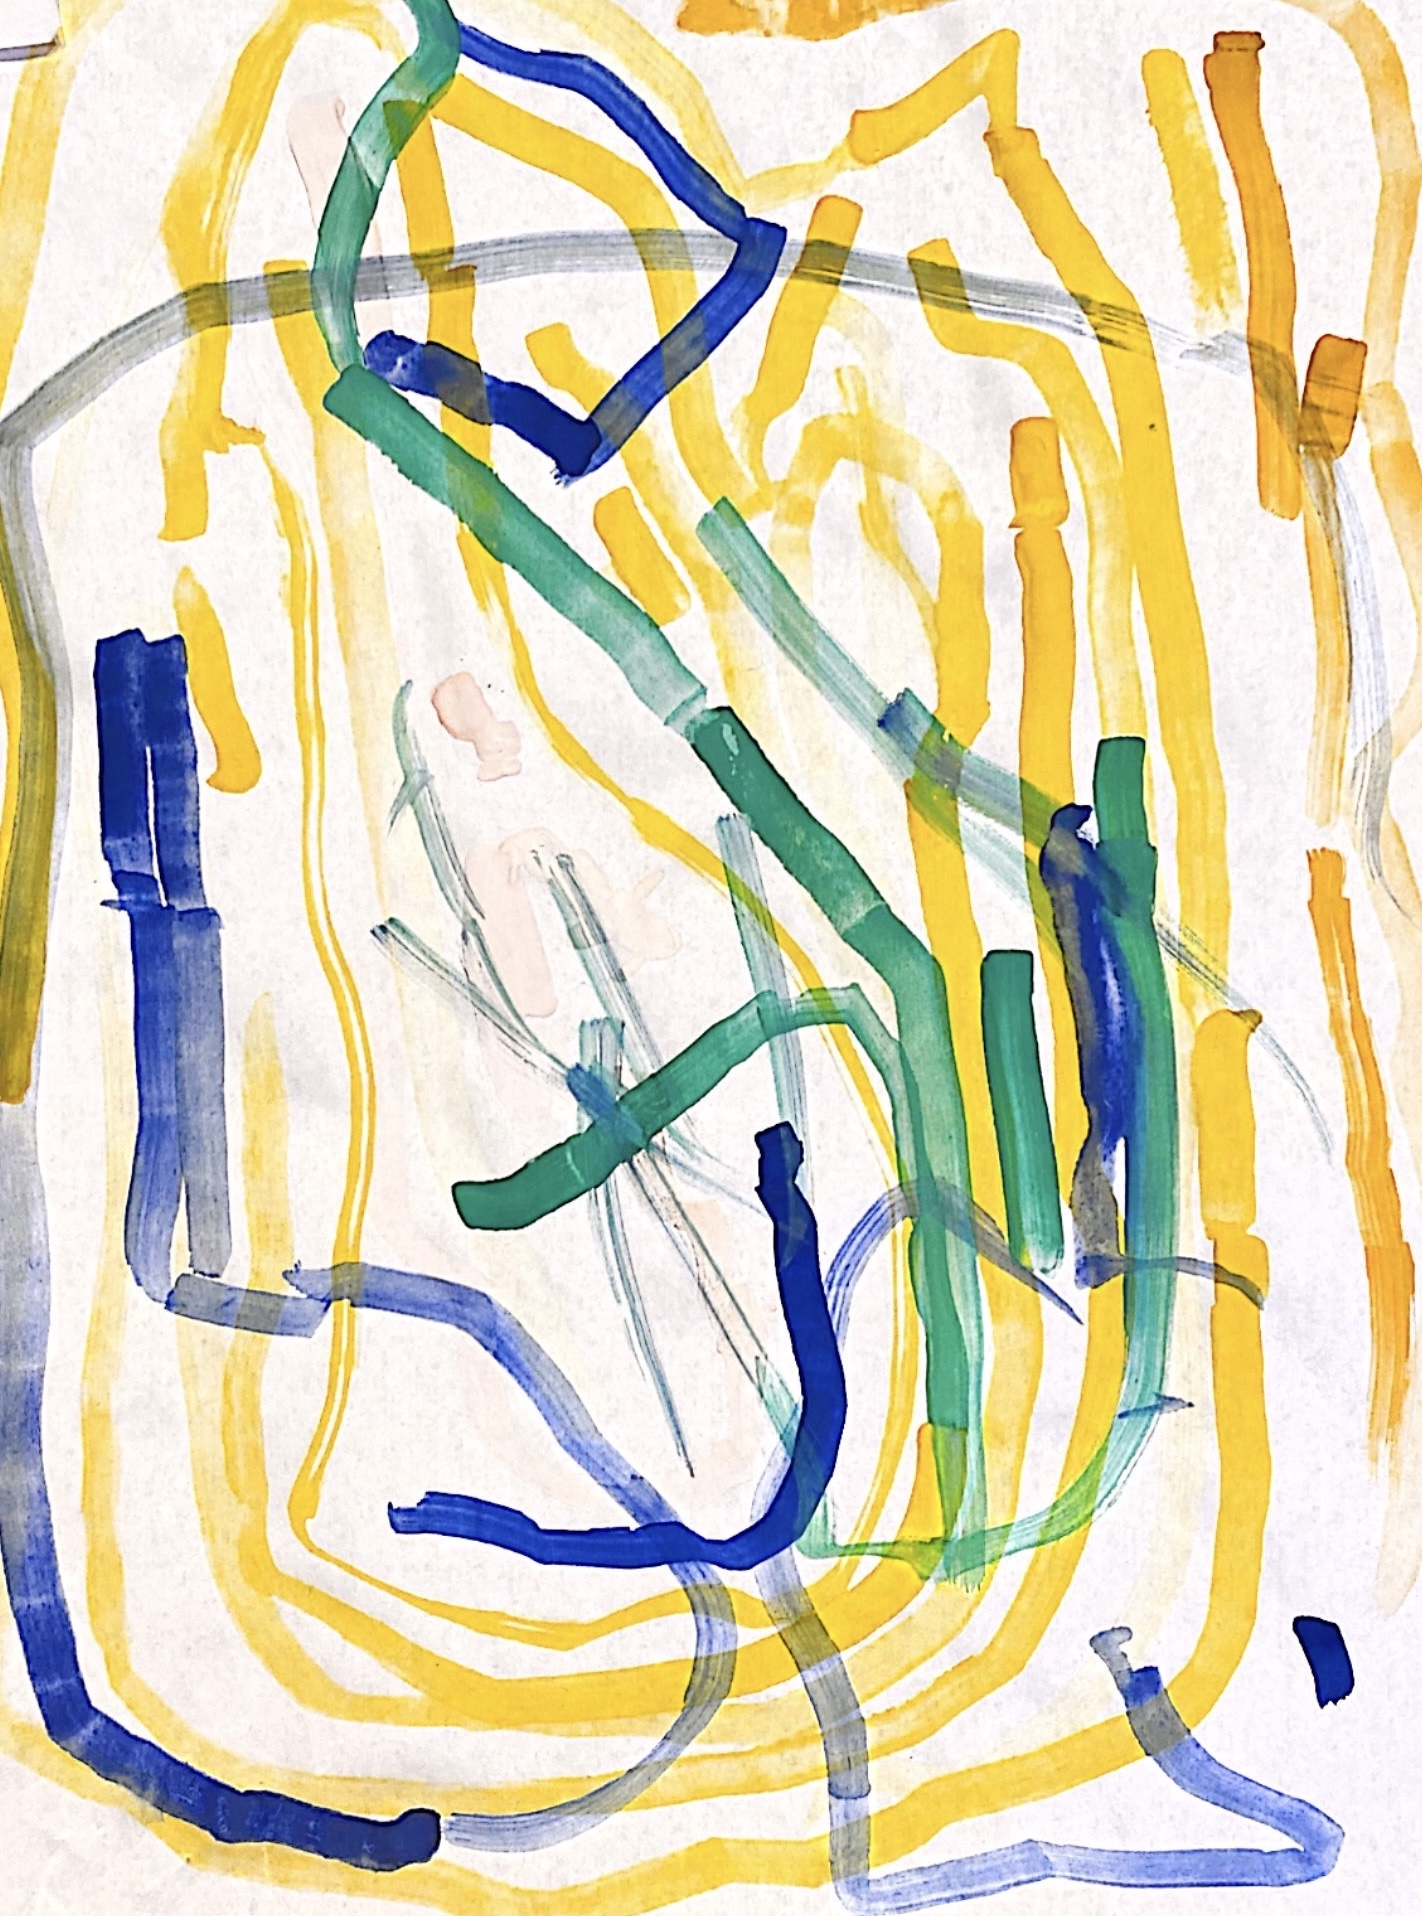
\includegraphics[width=\textwidth]{cover.jpg}
\vspace{1cm}
\end{minipage}
\par
}
\makeatletter
\renewcommand{\@maketitle}{%
\thispagestyle{plain}%
\begingroup \topskip\z@skip
\null\vfil
\centering
\begingroup
\Huge\bfseries
\@title\par\vspace{24pt}%
\def\and{\par\medskip}\centering
\Large\mdseries\authors\par\bigskip
\endgroup
\vfil
\coverpic
\vspace{10cm}
\endgroup
\newpage
}
\makeatother

% Skip entry in TOC 
\DeclareRobustCommand{\gobblefive}[5]{}
\newcommand*{\SkipTocEntry}{\addtocontents{toc}{\gobblefive}}

% % Inkscape figures
% \usepackage{import,xifthen,pdfpages,transparent}

% \newcommand{\incfig}[2]{%
% \def\svgwidth{#2}
% \import{./fig/}{#1.pdf_tex}
% }

\numberwithin{section}{chapter}
\numberwithin{equation}{chapter}
\numberwithin{figure}{chapter}

%    For a single index; for multiple indexes, see the manual
%    "AMS Author Handbook, Monograph Classes", included in the
%    author package).
\makeindex

\begin{document}

\frontmatter

\title{Convex Optimization for Statistics and Machine Learning, Volume I:
  Analysis} 
\author{Ryan J.\ Tibshirani}

%    The 2010 edition of the Mathematics Subject Classification is
%    the current definitive version. 
%\subjclass[2010]{Primary }
%\keywords{}

\maketitle

%    Dedication.  If the dedication is longer than a few lines,
%    remove the centering instructions and the line break.
%\cleardoublepage
%\thispagestyle{empty}
%\vspace*{13.5pc}
%\begin{center}
%  Dedication text (use \\[2pt] for line break if necessary)
%\end{center}
%\cleardoublepage

\setcounter{page}{5} % Change page number to 7 if a dedication is present
\setcounter{tocdepth}{1} % Depth 1 means include sections
\tableofcontents

%    Include unnumbered chapters (preface, acknowledgments, etc.) here.
%\include{}

\mainmatter
%    Include main chapters here.

\part{Introduction}
\chapter{Why Read This Book?}
\label{chap:why_this_book}

\section{Why optimization?}

% Optimization lies at the heart of a lot of the methodology in machine learning 
% and computational statistics. A solid working knowledge of optimization is 
% important for students and researchers in machine learning. Clearly this would 
% help for computational purposes (knowing what optimization algorithms are
% applicable for any given problem, and why we might expect some to perform
% better or worse than others). Perhaps less expected, as we will see in later
% chapters in this book, knowledge of optimization will also help us to better
% understand the properties of machine learning methods (and even derive
% advanced statistical theory for them). For example, it would be hard to
% understand the basic properties of the lasso (least absolute shrinkage and
% selection operator) without understanding subgradients and the subgradient
% optimality condition; and it would be hard to understand support vector
% machines without understanding duality and the KKT (Karush-Kuhn-Tucker)
% conditions. 

\section{Why convexity?}

% What makes one optimization problem hard (intractable) and another easy
% (tractable)?  Of course, it is not possible to answer this question in full
% generality, but \emph{convexity} is now widely recognized as the most
% important single attribute that can distinguish a tractable optimization
% problem from an intractable one. We must be careful not to oversell this
% perspective: there certainly are some easy nonconvex problems, and some hard
% convex ones. But, if were to pick just a single problem attribute on which to
% place our bets, then convexity is probably the right one.

\paragraph{What about deep learning?}

\section{Why another book?}

\paragraph{What about algorithms?}

% Infrequently touched on here, but hinted at in several places. Algorithms will
% be at the center of Part II...
\chapter{How To Read This Book}

\section{Notation and conventions}

% essentially all notation defined in passing so that the book reads more
% fluidly, but everything is also defined here for completeness...

% affine vs linear (used interchangeably when we talk about functions), except
% we are sure to use affine subspace, and affine span/dependence

% analytical or closed-form solution: written in terms of functions and
% mathematical operations from a given generally-accepted set. (wikipedia defines
% the former to be broader than the latter, we use them synonomously)
% https://en.wikipedia.org/wiki/Closed-form_expression

% $\R^d$ denotes $d$-dimensional Euclidean space 
% all vectors are treated columns vectors, constructed as $x=(x_1,\ldots,x_d)$ 
% $\T$ is the transpose operator so $a^\T b$ is the standard inner product
% also write this as $\langle a, \rangle b$, etc etc

% $\one$ is used flexibly to denote 1s vector of whatever dimension

% $\geq$ is componentwise

% $1\{ ... \}$ indicator

% Notation: $x_1$ refers to the first component of $x$ or the first in a sequence
% of vectors, to be used flexibly 

% inf/sup written in two ways (sets versus operators)

% unless otherwise specified, sets are in euclidean space, functions act on
% euclidean space

% Definitions for MATRICES are not made separately from those over vector
% space. Interpret everything as a vector space. Optimization facts, subgradients,
% proximal operatotrs, etc. etc. Interpret l2 -> Froebnius, inner product, etc
% etc. 

% if statements are vacuous when conditions are vacuous, then ... be mature!
% e.g. we don't always explicitly rule out things like empty sets, functions
% that are identically infinite, etc. 

\section{Background level}

\section{Recommended paths}

%\include{} % what about deep learning

\part{Fundamentals}
\chapter{Convex Sets and Functions}
\label{chap:convex_sets_functions}

\section{Convex sets}  
\label{sec:convex_sets}

Convex sets are the main building blocks for the study of convex functions and
their properties. Essentially everything that can be said about convex
functions can be traced back to a statement about convex sets. A set $C
\subseteq \R^d$ is called \emph{convex} if it satisfies 
\index{convex set} 
\begin{equation}
\label{eq:convex_set}
x, y \in C \implies t x + (1-t) y \in C, \quad \text{for all $t \in [0,1]$}. 
\end{equation}
This says that the line segment $\{ tx + (1-t) y : t \in [0,1] \}$ joining $x$
and $y$ lies entirely in $C$. See Figure \ref{fig:convex_set}. A \emph{convex 
  combination} of points $x_1,\ldots,x_n \in \R^d$ is one of the form   
\index{convex combination} 
\[
\sum_{i=1}^n t_i x_i, \quad \text{where $t_i \geq 0$, for $i=1,\ldots,n$ and 
  $\sum_{i=1}^n t_i = 1$}. 
\] 
The \emph{convex hull} of $C$ is the set of all convex combinations of points in
$C$, 
\index{convex hull} 
\[ 
\conv(C) = \bigg\{
\sum_{i=1}^n t_i x_i : 
\text{$n \geq 1$, $x_i \in C$, $t_i \geq 0$, for $i=1,\ldots,n$, and 
  $\sum_{i=1}^n t_i = 1$} \bigg\}. 
\]
The convex hull $\conv(C)$ is itself a convex set, for any set $C$; in fact, it
is the smallest convex set containing $C$, meaning $\conv(C) \subseteq D$ for 
any convex set $D \supseteq C$. 

\begin{figure}[tb]
\centering
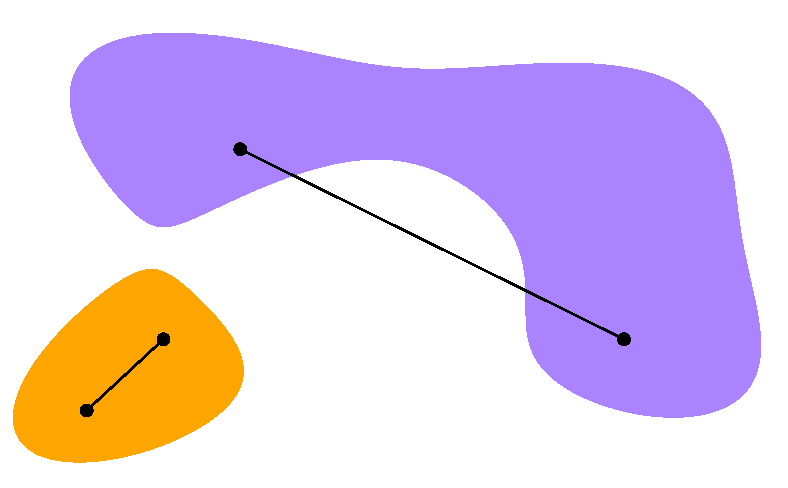
\includegraphics[width=0.65\textwidth]{fig/convex_set.pdf}
\caption{Lower left: convex set, such that the line segment joining any two 
  elements will lie entirely in the set. Upper right: nonconvex set, such
  that this does not hold.} 
\label{fig:convex_set}
\end{figure}

\begin{Example}
The following are examples of convex sets. 

\begin{enumerate}[label=\alph*.]
\item The empty set $\emptyset$, and all of Euclidean space $\R^d$. 

\item A line $\{x + t y : t \in \R\}$, ray $\{x + t y : t \geq 0\}$, and line  
  segment $\{x + t y : t \in [0,1]\}$.

\item A linear subspace $\{x : Ax = 0\}$, and affine subspace $\{x : Ax = b\}$. 

\item A hyperplane $\{x : a^\T x = b\}$, and halfspace $\{x : a^\T x \leq b\}$. 

\item A \emph{norm ball} $\{x : \|x\| \leq t\}$, where $\|\cdot\|$ is a norm on
  $\R^d$, and $t \geq 0$. 
  \index{norm!ball}
  
\item A \emph{polyhedron} $\{x: a_i^\T x \leq b_i, \, i=1,\ldots,m\}$. This is
  the intersection of a finite number of halfspaces. We can express this
  succinctly as $\{x : Ax \leq b\}$, where here and throughout we read the
  inequality componentwise.   
\end{enumerate}
\end{Example}  

It will be important to think about convexity for sets of matrices (and
convexity for functions of matrices), since some interesting optimization
problems are formulated over matrices. By viewing $\R^{k \times d}$---the space 
of real $k \times d$ matrices---as a vector space of dimension $kd$, everything   
we cover for convex sets in $\R^d$ (and convex functions on $\R^d$) can be
translated over to $\R^{k \times d}$. 

The same can be said about $\SS^d$---the space of symmetric real $d \times d$
matrices---which we can view as a vector space of dimension $d(d+1)/2$. A subset
of $\SS^d$ of particular interest is 
\index{positive semidefinite cone} 
\index{positive semidefinite matrix} 
\begin{equation}
\label{eq:psd_cone}
\SS_+^d = \{X \in \SS^d : X \succeq 0 \}.
\end{equation}
Here we write $X \succeq 0$ to denote that $X$ is \emph{positive semidefinite}:
it satisfies $a^\T X a \geq 0$, for all $a \in \R^d$. We call $\SS_+^d$ the
\emph{positive semidefinite cone} (of dimension $d$). This is a convex set,
indeed a \emph{convex cone} which means it satisfies $X,Y \in \SS^d \implies s
X + t Y \in \SS^d$ for all $s,t \geq 0$. To see this, note that for any $s, t
\geq 0$ and $a \in \R^d$, we have  
\[
a^\T (s X + t Y) a = s a^\T X a + t a^\T Y a \geq 0,
\] 
provided that $X,Y$ are positive semidefinite to begin with. 

Given a set $C$ and a point $x \in C$, another interesting convex cone is the
\emph{normal cone} to $C$ at $x$,   
\begin{equation}
\label{eq:normal_cone}
\cN_C(x) = \{ g : g^\T x \geq g^\T y, \, \text{for all $y \in C$}\}.
\end{equation}
For any set $C$ (convex or not), the associated normal cone $\cN_C(x)$ at 
any $x \in C$ is always a convex cone (which can be verified from the
definition). 
\index{normal cone} 

We finish this short section with two key theorems on properties of convex sets. 

\index{separating hyperplane theorem}
\begin{Theorem}[Separating hyperplane theorem]
\label{thm:separating_hyperplane}
If $C,D$ are nonempty disjoint convex sets, then there exists $a \not= 0$ and
$b$ such that $C \subseteq \{x : a^\T x \leq b\}$ and $D \subseteq \{x: a^\T x
\geq b\}$. The set $\{x : a^\T x = b\}$ is called a \emph{separating hyperplane} 
between $C,D$. 
\end{Theorem}

\index{supporting hyperplane theorem}
\begin{Theorem}[Supporting hyperplane theorem]
\label{thm:supporting_hyperplane}
If $C$ is a convex set and $x_0 \in \boundary(C)$ (the boundary of $C$), then
there exists $a \not= 0$ and $b$ such that $a^\T x_0 = b$ and $C \subseteq \{x :
a^\T x \leq b\}$. The set $\{x : a^\T x = b\}$ is called a \emph{supporting
  hyperplane} to $C$ at $x_0$. 
\end{Theorem}

The separating hyperplane theorem can be proved using basic arguments, and the
supporting hyperplane theorem can be proved from the separating hyperplane
theorem. These results are highly intuitive and the role of convexity can be
made clear pictorially, see Figure \ref{fig:set_theorems}. Furthermore, they
have important consequences in optimization. For example, the separating
hyperplane theorem can be used to prove what are called \emph{theorems of
  alternatives} (such as \emph{Farkas' lemma}); see Exercise
\ref{ex:farkas}. Also, the supporting hyperplane theorem can be used to prove
that subgradients always exist for a convex function (on the relative interior
of its effective domain); see Exercise \ref{ex:subgradient_existence}.

\begin{figure}[tb]
\centering
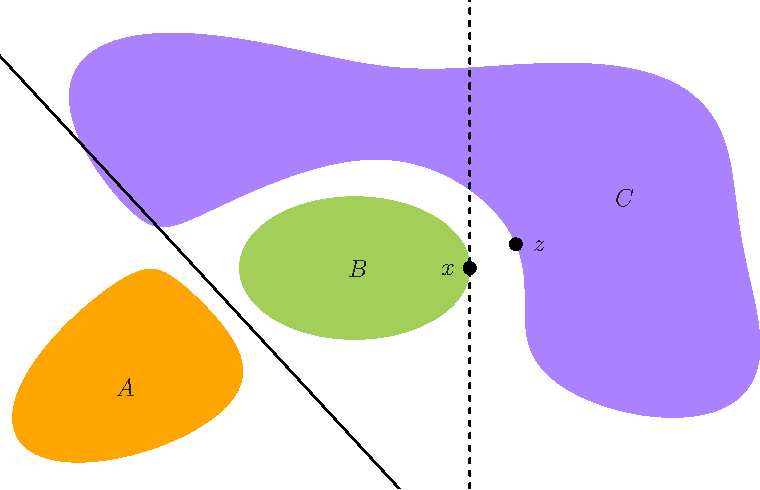
\includegraphics[width=0.675\textwidth]{fig/set_theorems.pdf}
\caption{Lower left, $A$ and $B$: two disjoint convex sets, which must hence 
  admit a separating hyperplane, illustrated as the solid line running between
  them. The set $B$, again by convexity, has a supporting hyperplane at every
  boundary point, illustrated by the dashed line supporting it at $x$. Upper
  right, $B$ and $C$: two disjoint sets which have no separating hyperplane,
  which is possible as $C$ is nonconvex. The set $C$ has no supporting
  hyperplane at $z$, possible again by nonconvexity.}   
\label{fig:set_theorems}
\end{figure}

\section{Convex functions}
\label{sec:convex_functions}

We now move from sets to functions, which may be a more familiar object of study
to some readers. For reasons that will be apparent, it is convenient to allow
functions to take both real and infinite values. Throughout, by default (without
further specification), a function is defined on all of $\R^d$ and takes values
in the \emph{extended real numbers} $[-\infty, \infty]$. For such $f : \R^d \to
[-\infty, \infty]$, we denote
\index{effective domain}
\[
\dom(f) = \{x : f(x) < \infty \},
\]
and call this set the \emph{effective domain} of $f$. Note that, as we are
allowing functions to take infinite values, there is no loss of generality in
considering functions defined on all of $\R^d$: given $S \subseteq \R^d$ and $f
: S \to [-\infty, \infty]$, we can always be extend $f$ to all of $\R^d$ by
setting it equal to $\infty$ outside of $S$.

We say that $f : \R^d \to (-\infty, \infty]$ is \emph{convex} if $\dom(f)$ is a
convex set and  
\index{convex function} 
\index{strict convexity}
\begin{equation}
\label{eq:convex_function}
f \big(t x + (1-t) y \big) \leq t f(x) + (1-t) f(y),  \quad \text{for all $x,y
  \in \dom(f)$ and $t \in [0,1]$}. 
\end{equation}
This says that the line segment joining $(x,f(x))$ and $(y,f(y))$ lies above  
the graph of $f$, as shown in Figure \ref{fig:convex_function}. We call  
$f$ \emph{strictly convex} provided that strict inequality holds in the above
statement,  
\begin{equation}
\label{eq:strictly_convex_function}
f \big(t x + (1-t) y \big) < t f(x) + (1-t) f(y),  \quad \text{for all $x
  \not= y \in \dom(f)$ and $t \in (0,1)$}. 
\end{equation}
In a sense, this says that $f$ is ``more convex'' than a linear function, as a
linear function would (by definition) have equal left and right hand sides in
\eqref{eq:strictly_convex_function}. A stronger notion than strict convexity is
\emph{strong convexity}, which means, for a parameter $m>0$, the function $f_m$
defined by  
\index{strong convexity}
\[
f_m(x) = f(x) - \frac{m}{2} \|x\|_2^2
\]
is convex. Like strict convexity requires more curvature than a linear function,
strong convexity requires that $f$ be ``more convex'' than a quadratic function. 

A companion notion to convexity is \emph{concavity}. A function $f : \R^d \to  
[-\infty, \infty)$ is called \emph{concave} provided that $-f$ is convex, or
equivalently: $\dom(-f)$ is a convex set and  
\index{concave function} 
\begin{equation}
\label{eq:concave_function}
f \big(t x + (1-t) y \big) \geq t f(x) + (1-t) f(y),  \quad \text{for all $x,y
  \in \dom(-f)$ and $t \in [0,1]$}. 
\end{equation}
Similarly, we say that $f$ is \emph{strictly concave} or \emph{strongly concave}
provided that $-f$ is strictly convex or strongly convex, respectively.   

In general, when it is not clear from the context, we will say that $f$ convex
``on $C$\hspace{1pt}'' to indicate that we are interpreting its effective domain
to be $\dom(f) = C$ (think: we set $f$ to be $\infty$ outside of $C$), and
similarly for concave functions. 

\begin{figure}[tb]
\centering
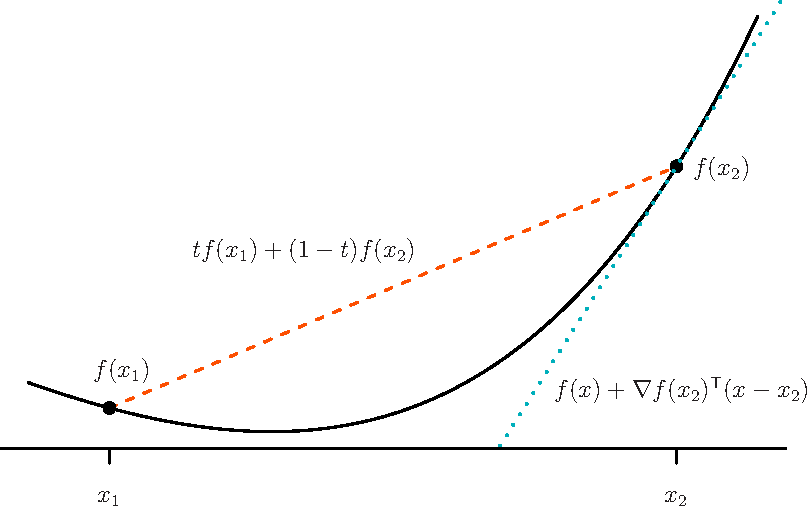
\includegraphics[width=0.7\textwidth]{fig/convex_function.pdf}
\caption{Convex function $f$, such that the line segment between any two points   
  on its graph lies above the function, as illustrated by the dashed line
  joining $(x_1,f(x_1))$ and $(x_2,f(x_2))$. Since $f$ is differentiable,
  convexity is equivalent to $f$ lying everywhere above its tangent line at any
  point, as illustrated by the dotted line running tangent to $f$ at $x_2$.}   
\label{fig:convex_function}
\end{figure}

\begin{Example}
The following are examples of convex or concave functions. In all cases, the
expressions should be interpreted as functions of $x$.

\begin{enumerate}[label=\alph*.]
\item The power function $x^a$ is convex on $\R_+=\{x : x \geq 0\}$ (the
  nonnegative real numbers) for $a \geq 1$, and concave on $\R_{++}= \{x : x > 0\}$
  (the positive real numbers) for $0 < a <  1$. It is also convex on $\R_{++}$
  for $a < 0$.

\item The exponential function $e^x$ is convex on $\R$. The logarithm function
  $\log(x)$ is concave on $\R_{++}$. The \emph{negative entropy} function $x
  \log(x)$ is convex on $\R_{++}$. 

\item A linear function $a^\T x + b$ is both convex and concave on $\R^d$. 

\item A quadratic function $\frac{1}{2} x^\T A x + b^\T x + c$ is convex on
  $\R^d$ for $A \succeq 0$ (positive semidefinite) and concave on $\R^d$
  for $A \preceq 0$ (negative semidefinite).

\item A norm $\|x\|$ is always convex. For example, on $\R^d$ we have the
  \emph{$\ell_p$ norms}, defined as: 
  \index{l1 norm@$\ell_1$ norm}
  \index{lp norm@$\ell_p$ norm}
  \index{linf norm@$\ell_\infty$ norm}
  \begin{align}
  \label{eq:lp_norm}
  \|x\|_p &= \bigg(\sum_{i=1}^d |x_i|^p\bigg)^{1/p}, 
  \quad \text{for $p \geq 1$}, \\
  \label{eq:linf_norm}
  \|x\|_\infty &= \max_{i=1,\ldots,d} \, |x_i|,
  \end{align}
  and on $\R^{k \times d}$ we have the \emph{trace norm} and \emph{operator 
    norm}, defined as: 
  \index{trace norm} 
  \index{operator norm}
  \begin{align}
  \label{eq:trace_norm}
  \|X\|_{\tr} &= \sum_{i=1}^k \sigma_i(X), \\
  \label{eq:operator_norm} 
  \|X\|_{\op} &= \sigma_1(X), 
  \end{align}
  respectively (these are also called the \emph{nuclear norm} and \emph{spectral  
    norm}, respectively). Here $\sigma_1(X) \geq \cdots \geq \sigma_k(X) \geq
  0$ denote the singular values of $X$.

\item The \emph{characteristic function} of a set $C$, 
  \index{characteristic function} 
  \begin{equation}
  \label{eq:characteristic_function} 
  I_C(x) = \begin{cases}
  0 & x \in C \\
  \infty & x \notin C
  \end{cases},
  \end{equation}
  is convex provided that $C$ is a convex set. 

\item The \emph{support function} of a set $C$, 
  \index{support function}
  \begin{equation}
  \label{eq:support_function}
  h_C(x) = \sup_{z \in C} \, z^\T x,
  \end{equation}
  is always convex (regardless of the set $C$).
\end{enumerate}
\end{Example}

An important property of convex functions is \emph{Jensen's inequality}, which
says that for a convex function $f : \R^d \to (-\infty, \infty]$ and a random 
variable $X$ that is supported on $\dom(f)$, we have     
\index{Jensen's inequality} 
\begin{equation}
\label{eq:jensen}
f( \E[X] ) \leq \E[ f(X) ],
\end{equation}
provided the expectations exist. Oppositely, if $f$ is concave then $f( \E[X]
) \geq \E[ f(X) ]$, again provided the expectations exist. These inequalities
can be seen as generalizations of the defining properties of convexity and
concavity, \eqref{eq:convex_function} and \eqref{eq:concave_function},
respectively, from discrete to arbitrary distributions.

\begin{Remark}
\label{rem:extended_value}
In this book, as per our definitions above, we do \emph{not allow convex
functions to take the value $-\infty$} and do \emph{not allow concave functions
to take the value $\infty$}. This is different from the approach taken by some
other authors and it excludes what are known as \emph{improper} convex functions
from consideration; see the chapter notes for further discussion. Restricting
convex and concave functions in this way will be sufficient for our purposes,
and simplifies matters that would otherwise require a more nuanced treatment.

\setlength{\parindent}{\normalparindent}
To see one advantage of restricting convex functions to take values in
$(-\infty, \infty]$, observe that for $f : \R^d \to (-\infty, \infty]$ with
$\dom(f)$ convex, we can equivalently write \eqref{eq:convex_function} as       
\[
f \big(t x + (1-t) y \big) \leq t f(x) + (1-t) f(y),  \quad \text{for all $x,y
  \in \R^d$ and $t \in [0,1]$}.  
\]
(This is possible because we never encounter the undefined expressions $\infty -
\infty$ or $-\infty + \infty$ in the above statement, as $f$ cannot take the 
value $-\infty$.) This offers an alternative view for convexity, based on
well-defined arithmetic within the extended real numbers, that can be more
fluid when working with functions that can take infinite values.
\end{Remark}

\section{Equivalent characterizations}
\label{sec:equivalent_characterizations}

There are a number of interesting alternative characterizations of convexity for
functions (conditions other than the definition that are either equivalent to
convexity or imply convexity), outlined next. 

\paragraph{Epigraph characterization.} 

A function $f : \R^d \to (-\infty, \infty]$ is convex if and only if 
\index{epigraph}
\begin{equation}
\label{eq:epigraph}
\epi(f) = \{ (x,t) \in \dom(f) \times \R : f(x) \leq t \},
\end{equation}
called its \emph{epigraph}, is a convex set. 
  
\paragraph{Lines characterization.} 

A function $f : \R^d \to (-\infty, \infty]$ convex if and only if the
restriction of $f$ to every line is convex, that is, the function $g(t) = f(x +
tv)$ is convex on $\{t : x + tv \in \dom(f)\}$ for all $x,v \in \R^d$.   

\paragraph{First-order characterization.} 

A differentiable function $f : \R^d \to (-\infty, \infty]$ is convex if and only
if $\dom(f)$ is convex and  
\begin{equation}
\label{eq:first_order_characterization}
f(y) \geq f(x) + \nabla f(x)^\T (y-x), \quad \text{for all $x,y \in \dom(f)$},  
\end{equation}
where $\nabla f(x)$ denotes the gradient of $f$ at $x$. This says that
first-order Taylor approximation to $f$ around any point $x$ must
globally under-approximate $f$; this is illustrated in Figure
\ref{fig:convex_function}. A similar result holds for strict convexity: a
differentiable function $f : \R^d \to (-\infty, \infty]$ is strictly convex if
and only if $\dom(f)$ is convex and 
\[
f(y) > f(x) + \nabla f(x)^\T (y-x), \quad \text{for all $x \not= y \in
  \dom(f)$}.   
\]
 
\paragraph{Second-order characterization.} 

A twice differentiable function $f : \R^d \to (-\infty, \infty]$ is convex if
and only if $\dom(f)$ is convex and  
\begin{equation}
\label{eq:second_order_characterization}
\nabla^2 f(x) \succeq 0, \quad \text{for all $x \in \dom(f)$},
\end{equation}
where $\nabla^2 f(x)$ denotes the Hessian of $f$ at $x$. This condition says
that the function $f$, at any point $x$, must be ``curved upwards'' in any
direction; more precisely, for $v \in \R^d$, letting $g(t)=f(x+tv)$, we see
that $g''(0) = v^\T \nabla^2 f(x) v \geq 0$ (by positive semidefiniteness). For
twice differentiable $f : \R^d \to (-\infty, \infty]$, if $\dom(f)$ is convex
and     
\[
\nabla^2 f(x) \succ 0, \quad \text{for all $x \in \dom(f)$},
\]
meaning $\nabla^2 f(x)$ is positive definite for all $x \in \dom(f)$, then $f$
is strictly convex. However, we note that this is \emph{not} a necessary   
condition; for example, $f(x) = x^4$ is strictly convex but $f''(0)=0$. 

\medskip

For concavity, each of the above equivalent characterizations has an analog
(we just apply the characterization to $-f$). For alternative
characterizations of strong convexity, see Theorem \ref{thm:strong_convexity}. 

\begin{Example} 
The convexity or concavity of the following two functions can be confirmed
using the second-order characterization
\eqref{eq:second_order_characterization}. 

\begin{enumerate}[label=\alph*.]
\item The \emph{log-sum-exp function}, defined by 
  \index{log-sum-exp function} 
  \[
  f(x) = \log\bigg( \sum_{i=1}^d e^{x_i} \bigg),
  \]
  is convex on $\R^d$.

\item The \emph{log-det function}, defined by $f(X) = \log(\det(X))$, is concave
  on $\SS_{++}^d = \{X \in \SS^d : X \succ 0\}$ (the space of positive definite
  $d \times d$ matrices). 
  \index{log-det function} 
\end{enumerate}
\end{Example}

\section{Operations preserving convexity}
\label{sec:operations_preserving_convexity}

To check the convexity of a given set or function, we can of course apply the
definition directly, or for functions, we can appeal to the alternative
characterizations from Chapter \ref{sec:equivalent_characterizations}. For
complicated sets or functions, this can become tedious. It is often easier to
instead (a) memorize a few key base examples of convex sets and functions (for
example, those given in Chapters \ref{sec:convex_sets} and
\ref{sec:convex_functions}), and (b) remember that various transformations
preserve convexity (as we will detail below). Then, checking convexity for a
given set or function becomes a task of trying to relate it to one of the key
base examples by one (or any sequence of) convexity-preserving transformations.

Here are some useful operations that preserve convexity for sets.

\paragraph{Intersection.} 
\parlab{par:set_intersection} 

If $C_s$ is convex for each $s \in S$, then the intersection \smash{$\cap_{s \in
    S} \, C_s$} is convex. 

\paragraph{Scaling and translation.} 

If $C \subseteq \R^d$ is convex, $a \in \R$, and $b \in \R^d$, then 
\[
aC+b = \{ ax + b : x \in C \}
\]
is convex.

\paragraph{Linear images and preimages.} 
\parlab{par:set_linear}

If $C \subseteq \R^d$ is convex and $f(x)=Ax+b$ for $A \in \R^{k \times d}$ and
$b \in \R^k$, then the image of $C$ under $f$, 
\[
f(C) = \{ f(x) : x \in C \}
\]
is convex. Also, if $D \subseteq \R^k$ is convex, then the preimage (or
inverse image) of $D$ under $f$,  
\[
f^{-1}(D) = \{ x : f(x) \in D \}
\]
is convex.

\paragraph{Perspective images and preimages.} 

The $(d+1)$-variate \emph{perspective function} is defined for $x \in \R^d$ and
$z>0$ as   
\index{perspective function}
\[
P(x,z) = x/z.
\]
Note $\dom(P)=\R^d \times \R_{++}$ (where recall $\R_{++}$ denotes the    
positive reals). If $C \subseteq \dom(P)$ is convex then the perspective image
$P(C)$ is convex; and if $D \subseteq \R^d$ is convex then the perspective
preimage $P^{-1}(D)$ is convex.  

\paragraph{Linear-fractional images and preimages.} 

A \emph{linear-fractional function} is the composition of a perspective function
with a linear function, that is, a function $f$ of the form      
\index{linear-fractional function} 
\[
f(x) = \frac{Ax + b}{c^\T x + e},
\]
with $\dom(f) = \{x : c^\T x + e > 0\}$. Supposing that $A \in \R^{k
  \times d}$, if $C \subseteq \R^d$ is convex and $C \subseteq \dom(f)$ then 
the linear-fractional image $f(C)$ is convex; and if $D \subseteq \R^k$ is 
convex then the linear-fractional preimage $f^{-1}(D)$ is convex.

\medskip

Here are now some useful operations that preserve convexity for functions (note
the analogy to the operations for sets, in many cases). 

\paragraph{Nonnegative linear combination.} 

If $f_1,\ldots,f_n$ are convex functions and $a_1,\ldots,a_n \geq 0$ then the
nonnegative linear combination $F = a_1f_1+\cdots+a_nf_n$, the function defined
as
\[
F(x) = a_1f_1(x) + \cdots + a_nf_n(x) 
\]
is convex.

\paragraph{Partial supremum.} 
\parlab{par:function_supremum}

Let $f$ be a function acting on a block variable $(x,z)$. If $f(\cdot,z)$ is
convex for each $z \in Z$ (meaning, $x \mapsto f(x,z)$ is convex), then the
partial supremum \smash{$F = \sup_{z \in Z} f(\cdot,z)$}, the function defined
as  
\index{partial supremum!convexity}
\[
F(x) = \sup_{z \in Z} \, f(x,z),
\]
is convex. An important special case, corresponding to a finite set $Z$: if
$f_i$, $i=1,\ldots,k$ are convex, then their pointwise maximum $F$, defined as
\smash{$F(x) = \max_{i=1,\ldots,k} \, f_i(x)$}, is convex.      

\paragraph{Partial infimum.} 
\parlab{par:function_infimum}

Let $f$ be a function acting on a block variable $(x,z)$. If $f$ is convex (to
be clear and to emphasize the difference to the above, here we mean $(x,z)
\mapsto f(x,z)$ is convex) and $Z$ is a convex set, then the partial infimum
\smash{$F = \inf_{z \in Z} f(\cdot,z)$}, the function defined as  
\index{partial infimum!convexity}
\[
F(x) = \inf_{z \in Z} \, f(x,z),
\]
is convex, provided that $F$ is nowhere equal to $-\infty$. 

\paragraph{Linear composition.} 
\parlab{par:function_linear}

Let $f : \R^k \to (-\infty, \infty]$ be convex, and let $A \in \R^{k \times d}$,
$b \in \R^d$. Then the function $F$ defined as $F(x) = f(Ax+b)$ is convex.     

\paragraph{Perspective transformation.} 
\parlab{par:function_perspective}

The \emph{perspective transform} of $f$ is the function defined as
\index{perspective transform}
\[
F(x,t) = t f(x/t),
\]
with $\dom(F) = \dom(f) \times \R_{++}$. If $f$ is convex, then so is its
perspective transform. 

\paragraph{General composition.} 
\parlab{par:function_composition}

Let $f : \R^k \to (-\infty, \infty]$, $g : \R^d \to \R^k$, and denote their
composition by $F = f \circ g$, that is, $F(x) = f(g(x))$. Then $F$ is convex if
$f$ is convex and, for each $i=1,\ldots,k$, either of the following holds (where
$g_i$ denotes the $i\th$ component function of $g$): 
\index{composition!convexity}
\begin{itemize}
\item $f$ is nondecreasing in its $i\th$ argument and $g_i$ is convex; or
\item $f$ is nonincreasing in its $i\th$ argument and $g_i$ is concave.
\end{itemize} 

To develop intuition for this rule, it helps to think of univariate twice
differentiable $f,g$ (though the rule of course applies more generally). In this
case, we can use the chain rule to compute
\[
F''(x) = f''(g(x)) (g'(x))^2 + f'(g(x)) g''(x).
\]
In order to have $F'' \geq 0$, we see that it suffices to have $f'' \geq 0$ and
$g'' \geq 0$ (that is, $f$ and $g$ convex) as well as $f' \geq 0$ (that is, $f$
nondecreasing). It would also work to have $f'' \geq 0$ and $g'' \leq 0$ (that
is, $f$ convex and $g$ concave) as well as $f' \leq 0$ (that is, $f$
nonincreasing).

\medskip

\begin{Example}
The following claims about convexity can be checked by identifying   
the right base examples and convexity-preserving transformations. 

\begin{enumerate}[label=\alph*.]
\item For $A_1,\ldots,A_d,B \in \SS^n$, the set $\{x : x_1 A_1 + x_2 A_2 +
  \cdots + x_d A_d \preceq B \}$ is convex.  

\item For $C \subseteq \R^d$ and a norm $\|\cdot\|$, the function giving the
  supremum distance to $C$,
\[
f(x) = \sup_{z \in C} \, \|x - z\|,
\]
is convex.

\item For $C \subseteq \R^d$ and a norm $\|\cdot\|$, the function giving the
  infimum distance to $C$,
\[
f(x) = \inf_{z \in C} \, \|x - z\|,
\]
is convex, provided that $C$ is convex.
\end{enumerate}
\end{Example}

Many common loss functions in statistical estimation and machine learning are
convex, and this can be readily checked using the results from this section or
the last; see Exercise \ref{ex:loss_functions}.             

\section{Smoothness and growth*}
\label{sec:smoothness_growth}

We say that a function $F$ is \emph{Lipschitz continuous} with parameter $L>0$
if 
\index{Lipschitz continuity}
\index{Lipschitz smoothness}
\[
\|F(x) - F(y)\|_2 \leq L \|x-y\|_2, \quad \text{for all $x,y \in
  \dom(f)$}. 
\]
We say that a function $f$ is \emph{Lipschitz smooth} with parameter $L>0$
provided $f$ is differentiable and its gradient $F=\nabla f$ satisfies the above
condition. 

Lipschitz continuity can be seen as a type of growth condition on the function
in question. To develop intuition for this, consider the case of a real-valued
function $F$: Lipschitz continuity means that, along any line segment, $F$
cannot grow faster than a linear function with slope $L$. Thus for real-valued $f$,
when $\nabla f$ is Lipschitz continuous ($f$ is Lipschitz smooth), one might
imagine that $f$ cannot grow faster than a quadratic function. The next
result makes this precise, and provides several other conditions related to
Lipschitz smoothness.

\index{Lipschitz smoothness}
\begin{Theorem}
\label{thm:lipschitz_smoothness}
For differentiable $f : \R^d \to (-\infty, \infty]$ and $L>0$, consider the
statements:  
\begin{enumerate}[label=(\roman*)]
\item $\|\nabla f(x) - \nabla f(y)\|_2 \leq L \|x-y\|_2$, for all $x,y \in
  \dom(f)$; 
\item the function $-f_L$ is convex, where $f_L(x) = f(x) - \frac{L}{2}
  \|x\|_2^2$;   
\item $f(y) \leq f(x) + \nabla f(x)^\T (y-x) + \frac{L}{2} \|y-x\|_2^2$, for all
  $x,y \in \dom(f)$;
\item $(\nabla f(x) - \nabla f(y))^\T (x - y) \leq L\|x-y\|_2^2$, for all $x,y
  \in \dom(f)$.
\end{enumerate}
Then the following relations hold: 
\[
\text{(i)} \implies \text{(ii)} \iff \text{(iii)} \iff \text{(iv)}. 
\]
If $f$ is twice continuously differentiable, then (ii)--(iv) are also equivalent
to the statement: 
\begin{enumerate}
\item[(v)] $\nabla^2 f(x) \preceq LI$, for all $x \in \dom(f)$.
\end{enumerate} 
Lastly, for convex $f$, statements (i)--(iv) are all equivalent, and for twice  
continuously differentiable convex $f$, statements (i)--(v) are all equivalent. 
\end{Theorem}

Interestingly, the concept of strong convexity admits a similar string of
equivalences. 

\index{strong convexity}
\begin{Theorem}
\label{thm:strong_convexity}
For differentiable $f : \R^d \to (-\infty, \infty]$ and $m>0$, consider the
statements:  
\begin{enumerate}[label=(\roman*)]
\item $\|\nabla f(x) - \nabla f(y)\|_2 \geq m \|x-y\|_2$, for all $x,y \in
  \dom(f)$; 
\item the function $f_m$ is convex, where $f_m(x) = f(x) - \frac{m}{2}
  \|x\|_2^2$;   
\item $f(y) \geq f(x) + \nabla f(x)^\T (y-x) + \frac{m}{2} \|y-x\|_2^2$, for all
  $x,y \in \dom(f)$;
\item $(\nabla f(x) - \nabla f(y))^\T (x - y) \geq m\|x-y\|_2^2$, for all $x,y
  \in \dom(f)$.
\end{enumerate}
Then the following relations hold: 
\[
\text{(i)} \impliedby \text{(ii)} \iff \text{(iii)} \iff \text{(iv)}. 
\]
If $f$ is twice continuously differentiable, then (ii)--(iv) are also equivalent
to the statement: 
\begin{enumerate}
\item[(v)] $\nabla^2 f(x) \succeq mI$, for all $x \in \dom(f)$.
\end{enumerate}
\end{Theorem}

Comparing Theorems \ref{thm:lipschitz_smoothness} and
\ref{thm:strong_convexity}, we might view Lipschitz smoothness and strong
convexity as dual concepts, informally speaking, since they give rise to
conditions that are symmetric in nature. (Perhaps not surprisingly, the proofs
of these conditions also proceed symmetrically, as outlined in Exercise
\ref{ex:lipschitz_smoothness}.)  In fact, as we will see later in Chapter 
\ref{sec:conjugates_smoothness}, there is a deeper (formal) dual relation at
play: Lipschitz smoothness of a function is intimately tied to strong convexity
of its conjugate.

Much of this chapter studies convex functions through the lens of their
gradients (or Hessians). Of course, a convex function need not be differentiable
(or twice differentiable). Take, for example, $f(x) = |x|$: convex, but not 
differentiable at $x=0$. Meanwhile, for a univariate convex function, the only
possibility for a point of nondifferentiability seems intuitively to be a
``kink'', like the behavior of the absolute value function at the origin. This
leads us to wonder, more generally: to what extent can a convex function lack
smoothness? Can a convex function be arbitrarily nonsmooth? Or does the property
of convexity impose restrictions on how ``much'' nondifferentiability is 
``allowed''? The next theorem answers this last question affirmatively. 

\index{Lipschitz smoothness} 
\index{Rademacher's theorem} 
\index{Aleksandrov's theorem} 
\begin{Theorem} 
\label{thm:smoothness_properties}
Let $f$ be a convex function. Then the following hold: 
\begin{enumerate}[label=(\roman*)]
\item $f$ is continuous at every point in $\interior(\dom(f))$;
\item in fact, $f$ is locally Lipschitz continuous on $\interior(\dom(f))$,
  meaning that for each compact set $C \subseteq \interior(\dom(f))$, there
  is a constant $L>0$ (this can depend on $C$) such that        
  \[
  |f(x) - f(y)| \leq L \|x-y\|_2, \quad \text{for all $x,y \in C$};
  \]
\item hence, $f$ is differentiable at almost every point in
  $\interior(\dom(f))$;   
\item moreover, $f$ is twice differentiable at almost every point in 
  $\interior(\dom(f))$.  
\end{enumerate}
\end{Theorem}

We remark that property (i) actually holds at every point in
$\relint(\dom(f))$, and we only write $\interior(\dom(f))$ in the theorem      
statement theorem to preserve symmetry in the presentation of
(i)--(iv). We also remark that property (iii) follows from (ii): that locally 
Lipschitz functions are differentiable almost everywhere is a result known as
\emph{Rademacher's theorem}. Property (iv), the almost everywhere twice
differentiability of convex functions, is known as \emph{Aleksandrov's
  theorem}. To be explicit, when we say that a certain property holds for almost 
every point in a set $S$, we mean that it holds on a set $E \subseteq S$ such
that $S \setminus E$ has Lebesgue measure zero.   

% Continuity: for example, Theorem 10.1 in Rockafellar (1970)
% Local Lipschitz: for example, Theorem 6.7 in Evans & Gariepy (2015) 
% Differentiability: for example, Theorem 6.6 in Evans & Gariepy (2015) 
% Twice differentiability: for example, Theorem 6.9 in Evans & Gariepy (2015) 
% Continuous differentiability (not relayed here): for example, Theorem 25.5 in
% Rockafellar (1970)?  

While the almost everywhere differentiability and twice differentiability of
convex functions is certainly interesting, we must be mindful not to
overinterpret the implications of Theorem \ref{thm:smoothness_properties} as
they pertain to convex optimization. Generally speaking, sets of Lebesgue
measure zero cannot be ignored in mathematical optimization (unlike, say,
functional analysis), particularly because many interesting optimization
problems lack smoothness at their minima; when this happens, as we will see in
the subsequent chapters, we must account for it, both analytically and 
algorithmically, and subgradients will be one of our primary tools for doing
so. 

\section{Cones and polyhedra*}
\label{sec:cones_polyhedra}

We cover cones and polyhedra in a bit more detail, two classes of sets that 
have special structure and play a central role in convex optimization. 

\subsection{Cones}
\label{sec:cones}

A set $C \subseteq \R^d$ is called a \emph{cone} if it satisfies 
\index{cone} 
\begin{equation}
\label{eq:cone}
x \in C \implies t x \in C, \quad \text{for all $t \geq 0$}.
\end{equation}
A special type of cone of particular interest is a \emph{convex cone}, which is
simply a set that is both a cone and convex. Combining \eqref{eq:convex_set} and
\eqref{eq:cone}, we see that a convex cone $C$ is defined by 
\index{convex cone}  
\begin{equation}
\label{eq:convex_cone}
x, y \in C \implies s x + t y \in C, \quad \text{for all $s, t \geq 0$}.
\end{equation}
Recall that the positive semidefinite cone \eqref{eq:psd_cone} and normal cone
\eqref{eq:normal_cone} are both convex cones. Another noteworthy example
is the \emph{norm cone}, defined for a norm $\|\cdot\|$ by 
\index{norm!cone}  
\begin{equation}
\label{eq:norm_cone}
\{ (x,t) \in \R^d \times \R : \|x\| \leq t \}.
\end{equation}

The \emph{conic hull} of $C$ is the set of all nonnegative linear combinations
of points in $C$,   
\[ 
\cone(C) = \bigg\{
\sum_{i=1}^n t_i x_i : 
\text{$n \geq 1$, $x_i \in C$, $t_i \geq 0$, for $i=1,\ldots,n$} \bigg\}. 
\]
The conic hull $\cone(C)$ is itself a convex cone, for any set $C$; in fact, it
is the smallest convex cone containing $C$, meaning that $\cone(C) \subseteq D$ 
for any convex cone $D \supseteq C$. 

Next we present a classical result on conic and convex hulls.

\index{Carath\'{e}odory's theorem}
\begin{Theorem}[Carath\'{e}odory's theorem]
\label{thm:caratheodory}
Let $C \subseteq \R^d$.

\begin{enumerate}[label=(\roman*)]
\item Every nonzero element in the conic hull $\cone(C)$ can be represented as a
  positive linear combination of linearly independent (and thus at most $d$)
  elements of $C$.  

\item Every element in the convex hull $\conv(C)$ can be represented as a convex
  combination of affinely independent (and thus at most $d+1$) elements of $C$.  
\end{enumerate}
\end{Theorem}

% Note: typical proof of convex hull result, using conic hull result, implies
% affine independence (though this isn't typically stated)

This has various important implications; see part f of Exercise
\ref{ex:convex_closed} for a basic one. 

\subsection{Polyhedra}
\label{sec:polyhedra}

A \emph{polyhedron} $P \subseteq \R^d$ is the intersection of a finite number of
halfspaces, which we can express generically as 
\index{polyhedron}
\[
P = \{x : Ax \leq b\}
\] 
for a matrix $A$ and vector $b$, where recall we interpret this inequality
componentwise. It should be clear that $\{x : Ax \geq b\}$, $\{x : \ell \leq Ax
\leq u\}$, and $\{x : Ax \leq b, \, Gx = h\}$ are all also polyhedra, as we
can rewrite each of them in the form of the above display, for appropriately
(re)defined $A,b$.

Less obvious is the fact that an optimization problem over a polyhedron can
always be equated with a higher-dimensional optimization problem over the
intersection of an affine subspace and the nonnegative orthant, $\{x : Ax=b, \,
x \geq 0 \}$. We will revisit this when we discuss linear programs in standard
form, in Chapter \ref{sec:linear_programs}. 

We call a bounded polyhedron a \emph{polytope}. A fundamental fact about
polytopes is as follows. 
\index{polytope} 

\begin{Theorem}
\label{thm:v_representation}
Every polytope can be represented as the convex hull of a finite set of points. 
\end{Theorem}

% For example, Theorem 3 page 32 in Grunbaum (2003)

This result is both highly intuitive and highly nontrivial; later, in Chapter
\ref{sec:dual_cones_polar_sets}, we will return to it from the perspective of
duality. Now we simply introduce some nomenclature to help
remember Theorem \ref{thm:v_representation}: we call $P = \{x : Ax \leq
b\}$ a \emph{halfspace representation} or \emph{H-representation} of $P$, and $Q
=  \conv\{x_1,\ldots,x_n\}$ a \emph{vertex representation} or  
\emph{V-representation} of $Q$. Then in this language, the theorem 
says that every polytope has an equivalent H-representation and
V-representation.   

An interesting aspect of polyhedra is their facial structure. A \emph{face} $F$
of a polyhedron $P \subseteq \R^d$ is a set $F$ such that 
\index{polyhedron!face}
\index{polyhedron!vertex}
\index{convex set!exposed point}  
\[
\text{$F = \emptyset$, $F = P$, or $F = P \cap H$ for a supporting hyperplane
  $H$ of $P$}. 
\]
The faces $F=\emptyset$ and $F=P$ are said to be \emph{improper}; each other
face of $F$ of $P$ is called \emph{proper}. A face $F$ is said to have dimension
$k$ (or, called a $k$-face) if its affine span $\aff(F)$ is $k$-dimensional. A
maximal proper face (proper face of maximum degree) of $P$ is called a
\emph{facet} of $P$. If $F=\{x\}$ is a $0$-face of $P$, then we call $x$ an
\emph{vertex} of $P$. 

To be fair, these concepts are not specific to polyhedra and the same
definitions apply to convex sets in general. A small difference in
nomenclature: if $F = \{x\}$ is a $0$-face of a convex set $C$, then we call $x$
an \emph{exposed point} of $C$ (for polyhedra, vertices and exposed points 
are equivalent, but not in general). Even in the general convex setting, these
concepts lead to interesting developments; for example, for any compact (closed
and bounded) convex set $C$, 
\index{Straszewicz' theorem}   
\[
C = \closure\big(\conv\{x : \text{$x$ is an exposed point of $C$}\}\big),  
\]
% For example, Theorem 8 page 19 in Grunbaum (2003) 
a result called \emph{Straszewicz' theorem}. (For polytopes, the above is true
without the surrounding $\closure(\cdot)$ because the set of exposed
points---that is, the vertex set---is finite.) For more, see Exercise
\ref{ex:extreme_points}. 

What makes polyhedra so special, however, is the \emph{structure} exhibited by
their faces. The faces of a polyhedron $P$ obey a beautiful recursive 
structure: each face of a face of $P$ is also a face of $P$, each face of $P$
can be expressed as an intersection of facets of $P$, and so on. 
% For example, Theorem 1 page 26 and Theorem 5 page 27 in Grunbaum (2003) 
We will not go into this in any detail, but we will leverage the relationship
between faces of $P$ and faces of its dual polytope $P^*$ when we prove
Theorem \ref{thm:v_representation} in Chapter \ref{sec:dual_cones_polar_sets}. 

\SkipTocEntry\section*{Chapter Notes}

A lot can be said about convex sets and functions, far more than what is said in
this chapter. For readers seeking a more in-depth treatment, there are many
excellent references on the subject, for example, 
\cite{rockafellar1970convex} (Chapters 1--11, 17--22), \cite{boyd2004convex}  
(Chapters 2, 3), \cite{bertsekas2009convex} (Chapters 1, 2), to name just a
few. \cite{boyd2004convex} gives a particularly comprehensive treatment of  
operations that preserve convexity. For more details on the smoothness
properties of convex functions, we refer readers to \cite{rockafellar1970convex}
(Chapters 10, 25), or \cite{evans2015measure} (Chapters 6.3, 6.4). To learn
more about polyhedra and the study of their facial structure, a classic
reference is \cite{grunbaum2003convex}.      

As briefly discussed in Remark \ref{rem:extended_value}, our definition of a
convex function does not allow it to take the value $-\infty$ (and likewise, we
do not allow a concave function to take the value $\infty$). This is in
contradiction with the standard approach in convex analysis, for example
\cite{rockafellar1970convex, bertsekas2009convex} (but it is consistent with 
the approach of others, for example \cite{boyd2004convex}). The standard
approach in convex analysis allows a convex function to take values in
$[-\infty,\infty]$, and defines a \emph{proper} convex function $f$ as one
such that $f \not= \infty$ and $f > -\infty$ ($f$ is not identically $\infty$,
and never $-\infty$). While proper convex functions are the real topic of
interest, \emph{improper} convex functions do arise in various situations, and
there are some nontrivial improper convex functions that are not just
identically $\pm \infty$, for example
\[
f(x) = \begin{cases}
-\infty & \|x\| < 1 \\
0 & \|x\| = 1 \\
\infty & \|x\| > 1
\end{cases},
\]
for a norm $\|\cdot\|$. Thus, from a general mathematical perspective, it is
important to be able to deal with them. Altogether, for our purposes, we find it
simpler to rule them out completely, though we admit this does come with its own
set of drawbacks, for example we must occasionally add explicit qualifiers to
statements about certain functions lying above $-\infty$, as we did in Property 
\parref{par:function_infimum}, the convexity-preserving rule for a partial
infimum.

\clearpage

\begin{xcb}{Exercises}
\begin{enumerate}[label=\thechapter.\arabic*]
\settowidth{\leftmargini}{0.00.\hskip\labelsep}
\item Prove that if $X$ is a random variable supported on a convex set $C
  \subseteq \R^d$ (and $\E(X)$ exists) then $\E(X) \in C$.  

\index{convex function!sublevel set}
\item \label{ex:convex_sublevel}
  Show that if $f$ is a convex function, then $\{x : f(x) \leq t \}$, called the
  \emph{sublevel set} of $f$ at level $t$, is a convex set. Show that the
  converse is not true: give an example of a nonconvex function whose sublevel
  sets are convex (for all levels $t$).

\item \label{ex:convex_closed}
  We explore some of the differences between preserving convexity and closedness
  of sets. 

\begin{enumerate}[label=\alph*.]
\item Prove Property \parref{par:set_intersection}, that an intersection of
  (any number of) convex sets is convex.

\item Prove that the intersection of (any number of) closed sets is closed.

\item Prove Property \parref{par:set_linear}, that linear images and preimages
  of convex sets are convex. 

\item Show that the preimage of a closed set under a linear map is closed; but
  the image of a closed set under a linear map need not be closed (give a
  counterexample). 

\index{convex hull}
\item Give an example of a closed set whose convex hull is not closed. 
  
\index{Carath\'{e}odory's theorem}
\item Prove that the convex hull of a compact (closed and bounded) set is
  compact. Hint: use part (ii) of Carath\'{e}odory's theorem (Theorem
  \ref{thm:caratheodory}), and sequential compactness.   
\end{enumerate}

\item \label{ex:convex_flavors}
  We explore some properties of the various ``flavors'' of convexity.   

\begin{enumerate}[label=\alph*.]
\index{strict convexity}
\item Give an example of a strictly convex function that is not strongly
  convex. 
  
\index{strong convexity}
\item Give an example of a strongly convex function that is not differentiable. 

\item Give an example of a strictly convex function $f$ such that $f(x) \to
  -\infty$ as $\|x\|_2 \to \infty$. 

\item Prove that for any differentiable strongly convex function $f$, we must
  have $f(x) \to \infty$ as $\|x\|_2 \to \infty$. Hint: use part (iii) of Theorem
  \ref{thm:strong_convexity}.
  
  \smallskip
  Note: differentiability is not actually required here; strong convexity alone
  is enough as we can use part (iii) of Theorem
  \ref{thm:strong_convexity_nonsmooth}; see Exercise
  \ref{ex:strong_convexity_coercive}.  
\end{enumerate}

\index{composition!convexity}
\item \label{ex:function_composition} 
  We explore Property \parref{par:function_composition} from a few perspectives.   

\begin{enumerate}[label=\alph*.]
\item Prove Property \parref{par:function_composition} by verifying directly
  that $F$ satisfies the definition of convexity. 

\item Prove that the second bullet point in Property
  \parref{par:function_composition} can be collapsed into the first: if the
  conditions of the property hold, and there exists $i$ such that $f$
  nonincreasing in its $i\th$ argument and $g_i$ concave, then we can simply
  reparametrize by flipping the signs of the appropriate arguments/component
  functions so that we can write \smash{$F = \tilde{f} \circ \tilde{g}$} for
  \smash{$\tilde{f}$} nondecreasing in each argument, and \smash{$\tilde{g}$} 
  with all component functions convex. 

\item Prove that Property \parref{par:function_composition} can be extended to
  the case where $g$ takes infinite values, in the following way. If $f : \R^k
  \to (-\infty, \infty]$ is convex and nondecreasing in each argument, and $g :
  \R^d \to (-\infty, \infty]^k$ is convex in each component, then $F = f \circ
  g$ is convex, where we set $F(x) = \infty$ for any $x$ with at least one
  component equal to $\infty$.  
\end{enumerate}

\item \label{ex:loss_functions} 
  In this exercise, we practice checking convexity, focusing on functions that 
  commonly appear in statistical estimation and machine learning. In some 
  instances, it might be easiest to use convexity-preserving operations from 
  Chapter \ref{sec:operations_preserving_convexity}, in others, it might be
  easier to prove the given claim straight from the definition.

\begin{enumerate}[label=\alph*.]
\index{linear regression}
\item \emph{Linear regression loss.} Prove that $f(\beta) = \|y -
  X \beta\|_2^2$ is convex, for any $X \in \R^{n \times d}$ and $y \in \R^n$.  

\index{logistic regression}
\item \emph{Logistic regression loss.} Prove that \smash{$f(\beta) = -y^\T 
    X \beta + \sum_{i=1}^n \log(1+e^{x_i^\T \beta})$} is convex, for any $X \in 
  \R^{n \times d}$ and $y \in \{0,1\}^n$, where $x_i \in \R^d$, $i=1,\ldots,n$  
  denote the rows of $X$.
  
\item \emph{Hinge classification loss.} Prove that \smash{$f(\beta) =
    \sum_{i=1}^n (1 - y_i x_i^\T \beta)_+$} is convex, where $a_+ = \max\{a,
  0\}$, for any $x_i \in \R^d$, $i=1,\ldots,n$ and $y \in \{-1,1\}^n$, 

\item \emph{Kullback-Leibler divergence between discrete distributions.} Prove
  that 
  \index{Kullback-Leibler divergence} 
  \[
  f(p,q) = \sum_{i=1}^d p_i \log(p_i / q_i) 
  \]
  is a convex function of $(p,q) \in \{ x \in \R^{2d} : \one^\T x = 1, \, x >
  0\}$.

\item \emph{Gaussian log likelihood for precision matrix.} Prove that 
  \index{Gaussian likelihood}
  \[
  f(\Sigma^{-1}) = -\frac{n}{2} \log(\det(\Sigma)) - \frac{1}{2} \sum_{i=1}^n 
  (x_i-\mu)^\T \Sigma^{-1} (x_i-\mu)
  \]
  is a concave function of $\Sigma^{-1} \in \SS_{++}^d$ (the inverse
  covariance matrix, called the \emph{precision matrix}), for any $x_i \in
  \R^d$, $i=1,\ldots,d$ and $\mu \in \R^d$. Hint: use the relationship between
  $\det(A)$ and $\det(A^{-1})$ for an invertible matrix $A$, and also linearity
  of the trace operator $\tr(\cdot)$. 

\item Let $f$ be strictly convex with $\dom(f)=\R^d$. By Property
  \parref{par:function_linear}, the linear composition rule, we know that  
  $g(\beta) = f(X \beta)$ is convex for any $X \in \R^{n \times d}$. Prove 
  that $g$ is strictly convex if and only if $\rank(X)=d$. 
\end{enumerate}

\item Now we practice checking nonconvexity. In some cases, a counterexample to
  \eqref{eq:convex_function} should be simple to produce; in others, inspecting
  the second-order condition \eqref{eq:second_order_characterization} might be
  easier.  

\begin{enumerate}[label=\alph*.]
\item \emph{$\ell_0$ ``norm''.}  Prove that $f(x) = \|x\|_0$, where
  \index{l0 norm@$\ell_0$ norm}
  \begin{equation}
  \label{eq:l0_norm}
  \|x\|_0 = \sum_{i=1}^d 1\{x_i \not= 0\}
  \end{equation}
  is the $\ell_0$ ``norm'', is nonconvex over $\R^d$.

  \smallskip
  Note: we use quotation marks since $\|\cdot\|_0$ is not a norm (it lacks
  positive homogeneity) and calling it a \emph{pseudonorm} would be more
  appropriate; however, we adopt the common terminology henceforth and simply
  refer to it as a norm (without quotations).   

\item \emph{Matrix rank.} Prove that $f(x) = \rank(X)$ is nonconvex over $\R^{n
    \times d}$.   

\item \emph{Gaussian negative log likelihood for mean and variance.} Prove that  
  \[
  f(\mu, \sigma^2) = \log \sigma + \frac{(y - \mu)^2}{2\sigma^2}
  \]
  is nonconvex over $\R \times \R_{++}$.

\item \emph{Least squares for two-layer neural network.} Prove that 
  \index{neural network}
  \[
  f(W, u, v) = \sum_{i=1}^n \bigg( y_i - \sum_{j=1}^k v_j 
  \phi (w_j^\T x_i + u_j) \bigg)^2 
  \]
  is nonconvex over $\R^{k \times p} \times \R^k \times \R^k$, where $\phi : \R
  \to \R$ can be taken (for simplicity) to be twice differentiable and monotone.    
\end{enumerate}

\item \label{ex:farkas} 
  The following is a ``strict'' variant of the separating hyperplane theorem: if 
  $C,D$ are nonempty disjoint closed convex sets, and (say) $D$ is bounded, 
  then there exists $a \not=0 $ and $b$ such that 
  \index{separating hyperplane theorem!strict version}
  \[
  \text{$a^\T x > b$ for all $x \in C$ and $a^\T x < b$ for all $x \in D$},
  \]  
  % For example, see proof in Section 2.5.1 of Boyd & Vandenberghe (2004)
  that is, the hyperplane $\{x: a^\T x =  b\}$ strictly separates $C,D$. 
  Use this to prove \emph{Farkas' lemma}: given $A \in \R^{k \times d}$, $b \in 
  \R^k$, exactly one of the following statements is true: 
  \index{Farkas' lemma} 
  \begin{itemize}
  \item there exists $x \in \R^d$ such that $Ax=b$, $x \geq 0$;
  \item there exists $y \in \R^k$ such that $A^\T y \geq 0$, $y^\T b < 0$. 
  \end{itemize}
  Hint: take $C = \{Ax : x \geq 0\}$. 

\item \label{ex:subgradient_existence} 
  The following is a ``strict'' variant of the supporting hyperplane theorem: if 
  $C$ is convex and $x_0 \in \relbd(C)$, then there exists $a \not=0 $ and $b$ 
  such that $a^\T x_0 = b$ and 
  \index{supporting hyperplane theorem!strict version}
  \[
  \text{$a^\T x \leq b$ for all $x \in C$, with $a^\T x < b$ for $x \in
    \relint(C)$}, 
  \] 
  % Proof: with loss of generality, we can take $a \in \aff(C)$. (We just
  % reparametrize to the affine subspace and work in this new coordinate
  % system.) If $x \in \relint(C)$ with $a^\T x = b$, then for some $\delta > 0$
  % we have $x + \delta a \in C$ by definition of the relative interior, but
  % clearly $a^\T (x + \delta a) = b + \delta \|a\|_2^2$, which breaks the 
  % assumption that $C$ is in the halfspace. 
  where $\relbd(C)$ and $\relint(C)$ denote the relative boundary and relative 
  interior, respectively, of $C$. We will use this to prove the existence of
  (what will be later defined as) subgradients of a convex function, on the
  relative interior of its effective domain. 
  
\begin{enumerate}[label=\alph*.]
\item Let $f$ be a convex function and $x \in \relint(\dom(f))$. Prove that 
  $(x,f(x)) \in \relbd(\epi(f))$, where $\epi(f)$ is the epigraph of $f$, as
  defined in \eqref{eq:epigraph}. 
  
\item Apply the strict version of the supporting hyperplane theorem given above
  to prove that there exists some nonzero $a = (s,v) \in \R^d \times \R$ such
  that 
  \[
  s^\T x + v f(x) \geq s^\T y + v t, \quad \text{for all $(y,t) \in \epi(f)$},  
  \]
  with strict inequality when $f(y) < t$. 

\item Prove that we must have $v < 0$, thus by rescaling $(s,v)$ and rearranging 
  the last display,
  \[
  f(y) \geq f(x) + s^\T (y - x), \quad \text{for all $y \in \dom(f)$}, 
  \]
  which says that $s$ is a subgradient of $f$ at $x$, denoted $s \in \partial
  f(x)$, as we will learn later in Chapter \ref{sec:subgradient_definition}. 
  \index{subgradient!existence}
  
\item Prove that restricting $x \in \relint(\dom(f))$ is necessary in general
  for the existence of a subgradient, by giving an example where $f$ is convex, 
  $x \in \dom(f) \setminus \relint(\dom(f))$, but $f$ has no subgradients at
  $x$. Hint: for this example, we want the supporting hyperplane to $\epi(f)$ at
  $(x,f(x))$ to be vertically-oriented, so if $a = (s,v)$ denotes the normal
  vector to this hyperplane, then $v=0$.  
  % Example: $f(x) = -\sqrt{1-x^2}$ for $|x| \leq 1$, and $\infty$ otherwise. No
  % subgradients at $x = \pm 1$.
\end{enumerate}

\item \label{ex:gradient_monotonicity}
  Prove, using the first-order characterization for convexity 
  \eqref{eq:first_order_characterization}, that a differentiable convex function
  $f$ has a gradient $\nabla f$ that acts as a \emph{monotone operator}, which
  means that it satisfies  
  \begin{equation}
  \label{eq:gradient_monotonicity}
  \big(\nabla f(x) - \nabla f(y)\big)^\T (x - y) \geq 0, \quad \text{for all
    $x,y \in \dom(f)$}. 
  \end{equation}
  Prove that the converse is also true, for differentiable $f$: if $f$ satisfies
  the above property then it must be convex. Hint: set $g(t) = f(x + tv)$ for
  $v=y-x$ and $t \in [0,1]$, and consider what the monotone gradient condition
  implies about $g'(t)$.   

\item \label{ex:lipschitz_smoothness} 
  In this exercise, we will work through the proofs of Theorems
  \ref{thm:lipschitz_smoothness} and \ref{thm:strong_convexity}.    

\begin{enumerate}[label=\alph*.]
\item Beginning with Theorem \ref{thm:lipschitz_smoothness}, show 
  that $\text{(ii)} \iff \text{(iii)} \iff \text{(iv)}$ by invoking 
  equivalent characterizations of convexity (including
  \eqref{eq:gradient_monotonicity}). 

\item Show that $\text{(i)} \implies \text{(iv)}$ by the Cauchy-Schwarz
  inequality, which proves the first display in Theorem
  \ref{thm:lipschitz_smoothness}.  

\index{Lipschitz smoothness} 
\item When $f$ is twice continuously differentiable, show that $\text{(v)}
  \implies \text{(iii)}$ using a first-order Taylor expansion of $f$ with 
  remainder; show that $\text{(iv)} \implies \text{(v)}$ by expressing $\nabla^2
  f(x) h$ as the directional derivative of $\nabla f(x)$ in the direction $h$,
  applying (iv), and taking $h$ to be the top eigenvector of $\nabla^2
  f(x)$. This establishes the second part of Theorem
  \ref{thm:lipschitz_smoothness}. 

\item Moving now to Theorem \ref{thm:strong_convexity}, show that 
  $\text{(ii)} \iff \text{(iii)} \iff \text{(iv)}$ by invoking equivalent 
  characterizations of convexity (including
  \eqref{eq:gradient_monotonicity}). 

\item Show that $\text{(iv)} \implies \text{(i)}$ by the Cauchy-Schwarz
  inequality, which proves the first display in Theorem
  \ref{thm:strong_convexity}.  

\index{strong convexity}
\item When $f$ is twice continuously differentiable, show that $\text{(v)}
  \implies \text{(iii)}$ using a first-order Taylor expansion of $f$ with 
  remainder; show that $\text{(iv)} \implies \text{(v)}$ by expressing $\nabla^2
  f(x) h$ as the directional derivative of $\nabla f(x)$ in the direction $h$,
  applying (iv), and taking $h$ to be the bottom eigenvector of $\nabla^2
  f(x)$. This establishes the second part of Theorem
  \ref{thm:strong_convexity}. 

\item For convex $f$, prove the final part of Theorem
  \ref{thm:lipschitz_smoothness} by showing $\text{(iv)} \implies \text{(i)}$,
  using the following steps. First, define $F_x(z) = f(z) - \nabla f(x)^\T
  z$. Argue that $F_x$ satisfies (iv), and thus also satisfies (iii), that is,   
  \[
  F_x(z) \leq F_x(y) + \nabla F_x(y)^\T (z-y) + \frac{L}{2}\|z-y\|_2^2. 
  \]
  Minimize each side of the above display over $z$. (Hint: use the fact that a 
  differentiable convex function is minimized by setting its gradient to zero
  applied to each of the left- and right-hand sides separately.)
  % LHS is minimized when $z - y = (\nabla f(x) - \nabla f(y)) / L$
  % RHS is minimized when $z = x$
  Show that, after rearrangement, this yields
  \[
  f(y) \geq f(x) + \nabla f(x)^\T (y-x) + \frac{1}{2L}\|\nabla f(y) - \nabla
  f(x)\|_2^2. 
  \]
  Exchange the roles of $x,y$, and add the resulting statement to the above
  display to get
  \[
  \big(\nabla f(x) - \nabla f(y)\big)^\T (x - y) \geq \frac{1}{L}\|\nabla f(y) -
  \nabla f(x)\|_2^2. 
  \]
  Use Cauchy-Schwarz to conclude that $f$ is Lipschitz smooth, as desired.

  \smallskip
  A remark on the proof technique: there is an interesting parallel between the  
  argument here and that used to prove that the conjugate a strongly
  convex function is Lipschitz smooth; see Exercise
  \ref{ex:conjugates_smoothness}. The last display above is equivalent to the
  conclusion that the conjugate $f^*$ of $f$ is strongly convex with parameter 
  $1/L$. To check this, set $u = \nabla f(x)$, $v = \nabla f(y)$, and note
  that $\nabla f^*(u) = x$ and $\nabla f^*(v) = y$. In comparison, the argument
  in Exercise \ref{ex:conjugates_smoothness} starts with the premise of strong  
  convexity, and then proceeds in the other direction, by essentially reversing
  the steps in the above argument.    
\end{enumerate}

\item We explore Theorems \ref{thm:lipschitz_smoothness} and
  \ref{thm:strong_convexity} a bit further, to better understand their
  statements of results and the necessity of certain assumptions. 

\begin{enumerate}[label=\alph*.]
\item First, show that the conditions $L>0$, $m>0$ in the theorems are
  unnecessary, in the sense that the stated results still hold for $L=0$ and
  $m=0$. Hint: what is a Lipschitz smooth function with $L=0$? What is a 
  strongly convex function with $m=0$?

\item Next, show that each of the four statements, (ii)--(v), in Theorem 
  \ref{thm:strong_convexity} imply that $f$ is convex (meaning, convexity is 
  implicit in all of the equivalences/implications). 

\item Now, show that convexity is \emph{not} implied by any one of the five  
  statements, (i)--(v), in Theorem \ref{thm:lipschitz_smoothness}. 

\item Lastly, show that convexity of $f$ is indeed necessary for equating (i)
  with the rest of the statements in Theorem \ref{thm:lipschitz_smoothness}:
  give an example of a nonconvex function that satisfies one of (ii)--(v), but
  not (i).  
  % Example: $f(x) = -x^4$
  % Critical point! The typical proof that (v) implies (i) is based on the
  % mean-value theorem that leverages $\|\nabla^2 f(x)\|_2$ being equal to to
  % the max eigenvalue of $\nabla^2 f(x)$. This is NOT generally true unless
  % $\nabla^2 f(x)$ is positive semidefinite!  
\end{enumerate}
 
\index{convex set!extreme point}  
\item \label{ex:extreme_points}
  A point $x \in C$ is said to be an \emph{extreme point} of a convex set $C$ if
  \[
  x = t y + (1-t) z, \, t \in (0,1), \, y,z \in C \implies x = y = z.
  \]
  In other words, $x$ cannot lie in the relative interior of any line segment
  joining distinct points in $C$. In this exercise, we will explore the
  properties of extreme points and their differences to exposed points, which
  recall from Chapter \ref{sec:polyhedra}, are points $x \in C$ such that  
  \index{convex set!exposed point}
  \[
  \text{$\{x\} = C \cap H$ for a supporting hyperplane $H$ of $C$}.
  \]
  We will write $\mathrm{ext}(C)$ and $\mathrm{exp}(C)$ for the sets of extreme
  and exposed points, respectively, of $C$. Throughout this exercise we take $C$ 
  to be convex.

\begin{enumerate}[label=\alph*.]
\item Prove that if $F$ is a face of $C$ and $C$ is closed, then
  $\mathrm{ext}(F) = F \cap \mathrm{ext}(C)$. 

\item Prove that if $C$ is compact, then $C = \conv(\mathrm{ext}(C))$. Hint:
  note that $C \supseteq \conv(\mathrm{ext}(C))$ by the definition of extreme  
  points; for the other direction (the opposite containment), use induction on
  the dimension $d$ of $\aff(C)$ (for $d=1$, the only compact sets are closed
  bounded intervals) and use part a. 

\item Prove that $\mathrm{exp}(C) \subseteq \mathrm{ext}(C)$. 

\item Prove that this is not an equality in general, by giving an example such 
  that $\mathrm{exp}(C) \subsetneq \mathrm{ext}(C)$ (an example with extreme
  points that are not exposed).     
  % Example: a box joined on the right by a half disk. Like a "D" with flat
  % three sides. Upper right corner of the box is extreme but not exposed
\end{enumerate}

\smallskip
A note on Straszewicz' theorem, from Chapter \ref{sec:polyhedra}: we can
interpret this, in light of parts b, c, d, as saying that for any compact convex
set $C$, the set of exposed points $\mathrm{exp}(C)$ is dense in the set of
extreme points $\mathrm{ext}(C)$. For polytopes, these two sets are finite, and
hence must be equal, which gives us another way of understanding Theorem 
\ref{thm:v_representation}.  

\item Let $f$ be a convex function and $P \subseteq \dom(f)$ a polytope
  (bounded polyhedron). Prove that the maximum of $f$ over $P$ is attained by
  one of the vertices of $P$. Hint: use the V-representation for $P$ that we
  know exists from Theorem \ref{thm:v_representation} (that is, express $P$ as
  the convex hull of a finite set of vertices). 

\item \label{ex:convex_maximization}
  Let $f$ be a convex function and $C \subseteq \dom(f)$ be a compact convex
  set. As a generalization of the last exercise, show that the maximum of $f$
  over $C$ is attained by one of the extreme points of $C$. Hint: use Exercise
  \ref{ex:extreme_points} part b. 
\end{enumerate}
\end{xcb}
\chapter{Optimization basics}
\label{chap:optimization_basics}

Equipped with a working knowledge of convex sets and functions, the basic
principles of optimization are now within reach. 

\section{Optimization problems}
\label{sec:optimization_problems}

In this book, we denote an \emph{optimization problem} by 
\index{optimization problem} 
\begin{equation}
\label{eq:optimization}
\begin{alignedat}{2}
&\minimize_x \quad && f(x) \\
&\st \quad && g_i(x) \leq 0, \; i=1,\dots,m \\ 
& && h_j(x) = 0, \; j=1,\dots,k.
\end{alignedat}
\end{equation}
Here $f$, $g_i$, $i=1,\dots,m$, and $h_j$, $j=1,\dots,k$ are functions, from 
$\R^d$ to $[-\infty,\infty]$. In problem \eqref{eq:optimization}, the
minimization is implicitly restricted to the intersection of relevant effective
domains: 
\index{effective domain}  
\[
D = \dom(f) \cap \bigcap_{i=1}^m \dom(g_i) \cap \bigcap_{j=1}^k \dom(h_j).
\]
The function $f$ in \eqref{eq:optimization} is called the \emph{criterion} or 
\emph{objective}. A \emph{feasible point} is a point in $D$ such that all
constraints (inequality and equality constraints) are met in problem
\eqref{eq:optimization}. The infimal criterion value among all feasible points
is denoted   
\index{optimization problem!criterion} 
\index{optimization problem!feasible point}     
\[
f^\star = \inf \big\{ f(x) : x \in D, \, g_i(x) \leq 0, \, i=1,\dots,m, \,
h_j(x) = 0, \, j=1,\dots,k \big\},
\]
and called the \emph{optimal value} in \eqref{eq:optimization}. A feasible point 
that achieves the optimal value is denoted $x^\star$ (note that $f^\star =
f(x^\star)$), and is called a \emph{solution} or \emph{minimizer}. 
\index{optimization problem!optimal value} 
\index{optimization problem!solution}  

It is worth being clear at the outset that a solution need not exist in an
optimization problem in general. This can happen for two distinct reasons.
First, a solution never exists in an optimization problem that is
\emph{infeasible}, which means that it has no feasible points. In this case, we
set $f^\star = \infty$ by convention. A second, more interesting case: even in
a feasible optimization problem ($f^\star < \infty$), a solution fails to
exist when the optimal value $f^\star$ is not attained. For example, informally
speaking, this happens when the criterion is minimized ``somewhere off at
infinity'' (as in $f(x) = e^{-x}$). The existence of solutions (in feasible
optimization problems) is itself a rich topic, and is covered further in Chapter 
\ref{sec:existence_minima}.       

A \emph{convex optimization problem} is one of the form
\eqref{eq:optimization} such that $f$ and $g_i$, $i=1,\dots,m$ are all
convex functions, and $h_j$, $j=1,\dots,k$ are all affine functions. In other
words, the problem 
\index{convex optimization problem}
\begin{equation}
\label{eq:convex_optimization}
\begin{alignedat}{2}
&\minimize_x \quad && f(x) \\
&\st \quad && g_i(x) \leq 0, \; i=1,\dots,m \\ 
& && Ax = b,
\end{alignedat}
\end{equation}
is convex whenever $f$ and $g_i$, $i=1,\dots,m$ are convex (and $A$ and $b$ are 
arbitrary).

In general, we will say that two optimization problems are \emph{equivalent} if 
solutions of one can be computed from solutions of the other, and vice versa. 
Clearly, problem \eqref{eq:optimization} is equivalent to:
\index{optimization problem!equivalence of problems}
\begin{alignat*}{2}
&\maximize_x \quad && -f(x) \\
&\st \quad && g_i(x) \leq 0, \; i=1,\dots,m \\ 
& && h_j(x) = 0, \; j=1,\dots,k,
\end{alignat*}
As $f$ is convex if and only if $-f$ is concave, the convex minimization 
problem \eqref{eq:convex_optimization} is hence also equivalent to a concave 
maximization problem. In this book, we will use ``optimization'' to refer to
both minimization and maximization (and we carry all definitions and notations
introduced above over to maximization problems); likewise, we will use ``convex
optimization'' to refer to both convex minimization and concave maximization.     

\begin{Remark}
In statistics, we rarely denote the parameter in an optimization problem by $x$;
we typically use $\beta$ or $\theta$ (or something else, as $x$ is usually
reserved for an input feature vector). We also rarely denote the solution to an
optimization problem by $\beta^\star$ or $\theta^\star$; we commonly use
\smash{$\hbeta$} or \smash{$\htheta$}, as these are typically seen as estimates
of population-level parameters of interest. In this book, when discussing
abstract properties of mathematical optimization, we will adhere to the standard
notation in optimization, as demonstrated above; but when discussing problems in
statistics or machine learning, we will switch fluidly to the notation more
common in these fields. This should not cause any confusion, as the meaning
(for example, what is a parameter and what is a feature) should be clear from
the context.   
\end{Remark}

\begin{Example}
The following are examples of two central optimization problems in statistics  
and machine learning. Both problems are convex. 

\begin{enumerate}[label=\alph*., ref=\alph*]
\item Given responses $y_i \in \R$ and associated feature vectors $x_i \in
  \R^d$, for $i=1,\dots,n$, the \emph{least absolute selection and shrinkage
    operator (lasso)} is a sparse estimator of the coefficients $\beta$ in a
  linear model (to $y_i$ predict from $x_i^\T \beta$), defined by the
  optimization problem: 
  \index{lasso}
  \begin{equation}
  \label{eq:lasso_sum}
  \minimize_\beta \quad \frac{1}{2} \sum_{i=1}^n (y_i - x_i^\T \beta)^2 +  
  \lambda \sum_{j=1}^d |\beta_j|.
  \end{equation}
  Here $\lambda \geq 0$ is a tuning parameter governing the tradeoff between 
  goodness-of-fit (first term) and sparsity (second term). The above also has a
  more compact form, denoting by $y \in \R^n$ the response vector and $X \in
  \R^{n \times d}$ the feature matrix (whose $i\th$ row is $x_i^\T$):  
  \begin{equation}
  \label{eq:lasso}
  \minimize_\beta \quad \frac{1}{2} \|y - X \beta\|_2^2 + \lambda \|\beta\|_1. 
  \end{equation}
  For insight into the sparsity-inducing property of $\ell_1$ penalties, from
  the perspective of proximal mappings, see Chapter
  \ref{sec:proximal_optimality}.    

  \noindent
  Note: by default, we will always omit an intercept term in the lasso
  regression model as it can be accounted for by centering $y$ and each column
  of $X$, before solving \eqref{eq:lasso}; see Example \parref{xa:lasso_partial}
  for a generalization.   

\item Given class labels $y_i \in \{ -1, 1\}$ and feature vectors $x_i \in
  \R^d$, for $i=1,\dots,n$, the \emph{support vector machine (SVM)} is a
  large-margin linear classifier (to predict $y_i$ from the sign of $\beta_0
  + x_i^\T \beta$), defined by the optimization problem:   
  \index{support vector machine} 
  \begin{equation}
  \label{eq:svm}
  \begin{alignedat}{2}
  &\minimize_{\beta_0,\beta,\xi} \quad
  && \frac{1}{2} \|\beta\|_2^2 + C \sum_{i=1}^n \xi_i \\ 
  &\st \quad && y_i (\beta_0 + x_i^\T \beta) \geq 1-\xi_i, \;  i=1,\dots,n \\
  & && \xi \geq 0.
  \end{alignedat}
  \end{equation}
  Here $C \geq 0$ is a tuning parameter governing the tradeoff between the size
  of the margin (the first term above is actually the \emph{inverse} margin; see
  Exercise \ref{ex:svm_margin}) and violations to the margin condition (the
  second term is the sum of violation costs, and each violation is an instance  
  of a prediction $\beta_0 + x_i^\T \beta$ lying on the wrong side of the
  margin).               
\end{enumerate}
\end{Example}

It is helpful to introduce some additional notation for an optimization problem 
\eqref{eq:optimization} in which the criterion is identically zero $f(x)=0$ (or, 
equal to any finite constant). We call this a \emph{feasbility problem}. A
feasibility problem effectively seeks whether the constraints can be satisfied,
and if so, seeks any point $x^\star$ that is feasible. We write it as  
\index{feasibility problem} 
\begin{equation}
\label{eq:feasibility}
\begin{alignedat}{2}
&\find \quad && x \\
&\st \quad && g_i(x) \leq 0, \; i=1,\dots,m \\ 
& && h_j(x) = 0, \; j=1,\dots,k.
\end{alignedat}
\end{equation}
A \emph{convex feasibility problem} is one in which the constraint functions
satisfy the usual requirements: $g_i$, $i=1,\dots,m$ are convex and $h_j$,
$j=1,\dots,k$ are affine.   

\section{Properties of convex problems} 
\label{sec:properties_convex_problems}

Next we describe several important properies of convex optimization problems,
beginning with the most important one.

\paragraph{Local solutions are global solutions.} 
\parlab{par:convex_local}

A point \smash{$\bar{x}$} is called a \emph{local solution} of the problem
\eqref{eq:optimization} if it is feasible and there is some $\delta>0$ such that 
\index{optimization problem!local solution}  
\[
f(\bar{x}) \leq f(x), \quad \text{for all feasible $x$ such that
$\|x - \bar{x}\|_2 \leq \delta$}.
\]
For a convex optimization problem, the following holds: any local solution
\smash{$\bar{x}$} must also be a global solution, in that \smash{$f(\bar{x})
  \leq f(x)$} for all feasible points $x$. (This is also simply called a
solution, and we add the modifier ``global'' here to emphasize the difference to
the local condition.) This result is so important that it may as well be called
the \emph{fundamental theorem of convex optimization}. 

The proof of this fundamental result is elementary. It can be broken into two  
steps. The first step is to check that for the convex problem
\eqref{eq:convex_optimization}, the set of feasible points is a convex set,
which follows from convexity of the set $D$, convexity of the functions $f$ and
$g_i$, $i=1,\dots,m$, and the linear structure of the equality constraints 
$Ax=b$ (Exercise \ref{ex:convex_solution} part a).  

The second step proceeds by contradiction. If \smash{$\bar{x}$} is not a global
solution, then there is a feasible point $y$ such that \smash{$f(y) <
  f(\bar{x})$}. Since \smash{$\bar{x}$} is locally optimal, we must have
\smash{$\|y - \bar{x}\|_2 > \delta$}. However, we can choose some $t \in (0,1)$ 
such that \smash{$x = ty + (1-t) \bar{x}$} satisfies \smash{$\|x - \bar{x}\|_2
  \leq \delta$} (for example, take \smash{$t = \delta / \|y - \bar{x}\|_2$}).
By convexity of the feasible set, we know that $x$ is feasible. By convexity of
$f$,  
\[
f(x) \leq t f(y) + (1-t) f(\bar{x}) < f(\bar{x}),
\]
where the last inequality is strict since \smash{$f(y) < f(\bar{x})$} and
$t>0$. The above display is a contradiction of local optimality, which proves
that such a $y$ cannot exist, and \smash{$\bar{x}$} must be globally optimal. 

\paragraph{Solution sets are convex.} 
\parlab{par:convex_solution} 

A related property of a convex optimization problem is that its solution set,
which we can denote by 
\[
S^\star = \{ x^\star: \text{$x^\star$ is a solution in
  problem \eqref{eq:convex_optimization}} \},
\]
is itself a convex set. The proof is similar to the proof that the feasible set
of a convex problem is convex (Exercise \ref{ex:convex_solution} part b).
Convexity of $S^\star$ has the following interesting implication: a convex
problem can have 0, 1, or infinitely many solutions---no other number is
possible!  

An important refinement is possible when the criterion $f$ in a convex problem
is strictly convex. In this case, the solution set $S^\star$---if
nonempty---must be a singleton (Exercise \ref{ex:convex_solution} part d).
% In other words, for a convex optimization problem with strictly convex
% criterion, if a solution exists, then it must be unique.  
\index{convex optimization problem!uniqueness of solution}

\paragraph{First-order optimality condition.}
\parlab{par:first_order_optimality}   

Denote by 
\[
C = \{ x \in D : g_i(x) \leq 0, \, i=1,\dots,m, \, Ax = b \}
\]
the feasible set of the convex optimization problem
\eqref{eq:convex_optimization}. For a differentiable criterion $f$, a point $x
\in C$ is a solution if and only if 
\index{first-order optimality condition} 
\begin{equation}
\label{eq:first_order_optimality}
\nabla f(x)^\T (y - x) \geq 0, \quad \text{for all $y \in C$}.
\end{equation}
This is called the \emph{first-order optimality condition} for problem
\eqref{eq:convex_optimization}. It can be interpreted as follows: any move from 
$x$ in the direction of another feasible point cannot decrease the criterion
$f$, according to the first-order Taylor expansion of $f$ at $x$. In the
unconstrained case (which means $m=r=0$, so there are no constraints), the
feasible set is $C=\dom(f)$, and since a differentiable function has an open
effective domain (by assumption, see Appendix \ref{sec:derivative}), the
first-order optimality condition \eqref{eq:first_order_optimality} reduces to
the familiar zero gradient condition, often called \emph{Fermat's rule}:  
\begin{equation}
\label{eq:zero_gradient}
\nabla f(x) = 0.
\end{equation}
To see this observe that for sufficiently small $\delta>0$, we have $y = x +
\delta v \in \dom(f)$ for any $v$, which from  \eqref{eq:first_order_optimality}
leads us to the conclusion that $\nabla f(x)^\T v = 0$ for any $v$, implying
\eqref{eq:zero_gradient}.   

We note that the first-order optimality condition
\eqref{eq:first_order_optimality} is actually a special case of what we will
call the subgradient optimality condition, to be encountered later in Chapter  
\ref{sec:subgradient_optimality}. 

\begin{Example}
The following are three examples of the first-order optimality condition for
convex optimization. 

\begin{enumerate}[label=\alph*., ref=\alph*]
\item For a differentiable convex optimization problem with only equality
  constraints, 
  \[
  \minimize_x \quad f(x) \quad \st \quad Ax = b,
  \]
  the first-order optimality condition \eqref{eq:first_order_optimality} reduces
  to  
  \index{Lagrange multiplier condition} 
  \begin{equation}
  \label{eq:lagrange_multiplier}
  \nabla f(x) + A^\T v = 0, \quad \text{for some $v$}.
  \end{equation}
  The argument justifying \eqref{eq:lagrange_multiplier} is similar to that used
  in the unconstrained case to justify \eqref{eq:zero_gradient} (see Exercise
  \ref{ex:lagrange_multiplier}). The condition \eqref{eq:lagrange_multiplier}
  is known as a \emph{Lagrange multiplier condition}, and it will be generalized
  by the Karush-Kuhn-Tucker conditions, which we will study later in Chapter 
  \ref{chap:kkt_conditions}. 

\item The Euclidean projection operator $P_C$ onto a convex set $C \subseteq 
  \R^d$ can be formulated in terms of differentiable convex optimization. In 
  particular, for any $x \in \R^d$, its projection $P_C(x)$ onto $C$ is the
  unique solution of the optimization problem  
  \index{projection}
  \[
  \minimize_z \quad \|x - z\|_2^2 \quad \st \quad z \in C.
  \]
  The condition \eqref{eq:first_order_optimality} (now interpreted with respect
  to $z$) gives, after rearrangement,  
  \index{projection!variational inequality} 
  \begin{equation}
  \label{eq:variational_inequality}
  (x - z)^\T (z - y) \geq 0, \quad \text{for any $y \in C$}. 
  \end{equation}
  This is often referred to as the \emph{variational inequality} for a
  projection. It says that the vector pointing from $z$ to $x$ must have a
  positive inner product with the vector pointing from $y$ to $z$, for any $y
  \in C$. See Figure \ref{fig:variational_inequality}.    

\item \parlab{xa:zero_gradient_quadratic}
  For a convex quadratic function \smash{$f(x) = \frac{1}{2} x^\T A x + b^\T x
    + c$} (where $A \succeq 0$) the first-order optimality condition
  \eqref{eq:zero_gradient} says that $x$ minimizes $f$ if and only if
  \begin{equation} 
  \label{eq:zero_gradient_quadratic}
  Ax + b =  0
  \end{equation}
  We can now reason in cases. 
 \begin{enumerate}[label=(\roman*)]
 \item If $A$ is invertible, then the only solution to
   \eqref{eq:zero_gradient_quadratic} is $x^\star = -A^{-1} b$. 

\item If $A$ is singular and $b \in \col(A)$, then there are infinitely many
  solutions to \eqref{eq:zero_gradient_quadratic}, of the form $x^\star = x_0 +
  v$ where $x_0$ is one particular solution ($Ax_0 + b = 0$) and $v$ is any
  element in $\nul(A)$, the null space of $A$. 

 \item If $A$ is singular and $b \notin \col(A)$, then
   \eqref{eq:zero_gradient_quadratic} has no solution, which means that $f$ does
   not have a minimizer (it does not attain its infimum). An example in which
   this occurs is the 2-dimensional convex quadratic $f(x) = x_1^2 - x_2$. 
 \end{enumerate}
\end{enumerate}
\end{Example}

\begin{figure}[tb]
\centering
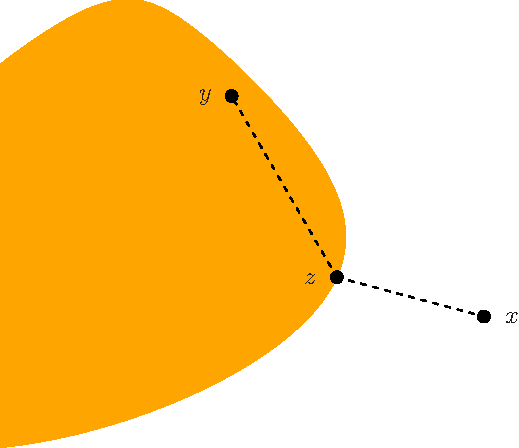
\includegraphics[width=0.475\textwidth]{fig/variational_inequality.pdf}
\caption{Illustration of the variational inequality that determines the
  optimality of the projection $z$ of a point $x$ onto a convex set. The angle
  between the line segments $zx$ and $zy$ must be at least a right angle (at
  least $90^\circ$), for any other point $y$ in the set.} 
\label{fig:variational_inequality}
\end{figure}

\section{Problem transformations}

We walk through various general transformations of optimization problems that
can make a problem easier to solve or easier to understand. In each case, we do
not assume convexity outright, but we do highlight the situations in which more
can be said about convex optimization.

\paragraph{Characteristic formulation.} 

Denote the feasible set of the optimization problem \eqref{eq:optimization} by  
\[
C = \{ x \in D : g_i(x) \leq 0, \, i=1,\dots,m, \, h_j(x) = 0, \, j=1,\dots,k
\} 
\]
Then \eqref{eq:optimization} is equivalent to the unconstrained optimization
problem 
\index{optimization problem!characteristic form}
\begin{equation}
\label{eq:characteristic_formulation}
\minimize_x \quad f(x) + I_C(x),
\end{equation}
where $I_C$ is the characteristic function of $C$, defined in
\eqref{eq:characteristic_function}. For convex optimization, recall that the
criterion $f$ and feasible set $C$ must both be convex, which implies 
$f + I_C$ is also convex. In others words, problem
\eqref{eq:characteristic_formulation} is convex provided that the original
problem \eqref{eq:optimization} is. 

We refer to \eqref{eq:characteristic_formulation} as the \emph{characteristic
  formulation} of problem \eqref{eq:optimization}. Though the characteristic 
formulation is not (typically) more practically convenient than the original
problem, it can still lead to useful insights. For example, in the convex case
(with $f$ and $C$ convex), applying the subgradient optimality condition to
\eqref{eq:characteristic_formulation} yields a natural generalization of the
first-order optimality condition in \eqref{eq:first_order_optimality}. This
will be covered in Chapter \ref{sec:subgradient_optimality}.

\paragraph{Partial optimization.} 
\parlab{par:partial_optimization}

For any function $g$, it holds that (Exercise \ref{ex:inf_sup_rules} part a):
\[
\inf_{x_1, x_2} \, g(x_1, x_2) = \inf_{x_1} \, G(x_1), 
\]
where $G(x_1) = \inf_{x_2} g(x_1,x_2)$. If we work from the characteristic
formulation \eqref{eq:characteristic_formulation}, for a general optimization
problem, and we treat $x$ as a block variable $x=(x_1,x_2)$, then we can apply
the above result to $g = f + I_C$: this tells us that we can perform
partial optimization---namely, optimization over $x_2$---to produce an
equivalent optimization problem, in $x_1$ alone. 

This statement can be made more concrete in the case that, for each fixed $x_1$,
the infimum of $g(x_1,x_2)$ over $x_2$ is attained, and we denote a
minimizer by $x^\star_2(x_1)$. Then $G(x_1) = g(x_1, x^\star_2(x_1))$, and 
\[
\minimize_{x_1,x_2} \quad f(x_1, x_2) \quad \st \quad (x_1,x_2) \in C, 
\]
is equivalent to 
\index{partial optimization}
\[
\minimize_{x_1} \quad F(x_1) \quad \st \quad x_1 \in \tilde{C},
\]
with \smash{$F(x_1) = \inf_{x_2 : (x_1,x_2) \in C} f(x_1,x_2) = f(x_1,
  x^\star_2(x_1))$}, and \smash{$\tilde{C} = \{x_1 : \text{$(x_1, x^\star_2  
    (x_1)) \in C$} \}$}. It is worth noting that the setting of convex
optimization, where $f$ and $C$ are convex in the former problem (second-to-last  
display), we know by Property \parref{par:function_infimum} that the latter
problem (last display) is also convex, provided that $F$ is nowhere equal to
$-\infty$.  

\begin{Example}
The following are two examples of partial optimization in convex problems. 

\begin{enumerate}[label=\alph*., ref=\alph*]
\item \parlab{xa:lasso_partial}
  For a response $y \in \R^n$, and features $X_1 \in \R^{n \times  d_1}$ and 
  $X_2 \in \R^{n \times   d_2}$, consider 
  \[
  \minimize_{\beta_1, \beta_2} \quad \frac{1}{2} \|y - X_1\beta_1 -
  X_2\beta_2\|_2^2 + \lambda \|\beta_1\|_1. 
  \]
  This is like the (usual form) lasso problem \eqref{eq:lasso}, but where the
  $\beta_2$ block of coefficients is not penalized. Since the above problem is
  simply a quadratic in $\beta_2$, we can minimize over it, for fixed $\beta_1$,
  and find that a minimizer \smash{$\hbeta_2(\beta_1)$} (which is unique if and
  only if $X_2$ is full column rank) satisfies       
  \[
  X_2 \hbeta_2(\beta_1) = P_{X_2} (y - X_1\beta_1)
  \]
  where \smash{$P_{X_2} = X_2 (X_2^\T X_2)^\pinv X_2$} is the projection onto
  $\col(X_2)$. By plugging this into the above original problem, we get an
  equivalent problem     
  \[
  \minimize_{\beta_1} \quad \frac{1}{2} \|P_{X_2}^\perp y - P_{X_2}^\perp
  X_1\beta_1\|_2^2+ \lambda \|\beta_1\|_1,  
  \]
  where \smash{$P_{X_2}^\perp = I - P_{X_2}$} is the projection onto the
  orthocomplement $\col(X_2)$. Note that this is a (usual form) lasso problem
  with response \smash{$P_{X_2}^\perp y$} and feature matrix
  \smash{$P_{X_2}^\perp  X_1$}.   

\item Consider the SVM problem \eqref{eq:svm}. Note that, after rearrangement,
  the linear constraints are equivalent to
  \[
  \xi_i \geq \big[1 - y_i(\beta_0 + x_i^\T \beta_0)\big]_+, \quad i=1,\dots,n, 
  \]
  where $a_+ = \max\{a,0\}$ denotes the positive part of $a$. Looking at the
  criterion in \eqref{eq:svm}, we can see that a minimizer over the $\xi$ block
  of variables, as a function of the others, achieves all equalities in the
  above set of inequalities (and this is unique if $C>0$): 
  \[
  \hat\xi_i(\beta_0,\beta) = \big[1 - y_i(\beta_0 + x_i^\T \beta_0)\big]_+,
  \quad i=1,\dots,n.
  \]
  This holds as increasing $\xi_i$ from \smash{$\hat\xi_i(\beta_0,\beta)$} by 
  any amount $\delta \geq 0$ increases the criterion by $C \delta \geq 0$.
  Plugging this in results in what is called the \emph{hinge form} of the SVM 
  problem: 
  \index{support vector machine!hinge form}
  \begin{equation}
  \label{eq:svm_hinge}
  \minimize_{\beta_0,\beta} \quad C \sum_{i=1}^n \big[1 - y_i(\beta_0 + x_i^\T 
  \beta)\big]_+ + \frac{1}{2} \|\beta\|_2^2.
  \end{equation}
  This has a familiar ``loss + penalty'' form, much like ridge regression, but
  with the hinge loss replacing what would be the squared loss in the ridge 
  regression problem. 
\end{enumerate}
\end{Example}

\paragraph{Monotone criterion transformation.} 
\parlab{par:monotone_transformation}

If $\phi$ is increasing then problem \eqref{eq:optimization}, with feasible set
abbreviated by $C$, is equivalent to 
\index{optimization problem!criterion transformation}
\[
\minimize_x \quad \phi(f(x)) \quad \st \quad x \in C,
\]
and hence also equivalent to, for any decreasing $\psi$,
\[
\maximize_x \quad \psi(f(x)) \quad \st \quad x \in C.
\]
It is worth noting that monotone transformations can influence convexity or
concavity in nontrivial ways. For example, \smash{$f(x) = e^{-x^2}$} is neither
convex nor concave, but for $\psi(u) = -\log(u)$ (decreasing) we get $\psi(f(x))
= x^2$, which is convex. Therefore it can be useful to apply a monotone
transformation to the criterion in an optimization problem, because it can turn
a nonconvex problem into a convex problem. An important example of this is
maximum likelihood estimation in log-concave families, as discussed in Chapter 
\ref{sec:maximum_likelihood}. 

It is also worth noting that monotone transformations can just as well be
applied in order to recast constraints; for example, if $\phi$ is increasing and
$\psi$ decreasing, then 
\[
g(x) \leq 0 \iff \phi(g(x)) \leq \phi(0) \iff \psi(g(x)) \geq \psi(0).
\]

\paragraph{One-to-one variable transformation.} 

If $\phi : \R^k \to \R^d$ is one-to-one (meaning, $u \not= v \implies \phi(u)
\not= \phi(v)$), and $\ran(\phi)$ contains the feasible set $C$ in problem
\eqref{eq:optimization}, then \eqref{eq:optimization} is equivalent to   
\index{optimization problem!variable transformation}
\[
\minimize_y \quad f(\phi(y)) \quad \st \quad \phi(y) \in C. 
\]
Such a variable transformation can be useful for various reasons: for example,
it can be dimension-reducing ($k < d$), or it can transform a nonconvex problem
into a convex one.  

\begin{Example}
An optimization problem with linear equality constraints,
\begin{alignat*}{2}
&\minimize_x \quad && f(x) \\
&\st \quad && g_i(x) \leq 0, \; i=1,\dots,m \\ 
& && Ax = b, 
\end{alignat*}
can always be recast, via variable transformation, into a problem with
inequality constraints only. Assuming $Ax = b$ has a solution $x_0$ (otherwise
the above problem is infeasible), we can parametrize the linear space of all 
solutions as $x = x_0 + Vy$, where the columns of $V \in \R^{d \times k}$ form
a basis for $\nul(A)$, and where $y \in \R^k$. Therefore the above problem is
equivalent to 
\begin{alignat*}{2}
&\minimize_y \quad && f(x_0+Vy) \\
&\st \quad && g_i(x_0+Vy) \leq 0, \; i=1,\dots,m.
\end{alignat*}
Though the above two problems are always equivalent, it is not always a good
idea (speaking practically) to seek to solve the second instead of the
first, and this is not a simple matter of comparing $k$ to $d$. Eliminating 
equality constraints can alter problem structure in nontrivial ways. For
example, if $A$ sparse, then it might not be easy (or even possible) to find a
sparse basis $V$ for $\nul(A)$, and such sparsity could be lost in moving
from the first problem to the second. This could make a big difference in
practice, depending on the specifics (the size of the problem, the algorithm 
one has in mind for computing a solution, etc.).
\end{Example}

\paragraph{Slack variables.} 

Proceeding in the opposite direction to the last example (eliminating equality
constraints), we can replace all of the inequality constraints in
\eqref{eq:optimization} with equality constraints, using the following
equivalent formulation:  
\begin{alignat*}{2}
&\minimize_{x,s} \quad && f(x) \\
&\st \quad && g_i(x) + s_i = 0, \; i=1,\dots,m \\ 
& && h_j(x) = 0, \; j=1,\dots,k, \\
& && s \geq 0.
\end{alignat*}
The variables $s_i$, $i=1,\dots,m$ here are called \emph{slack variables}. 
Comparing the above problem to \eqref{eq:optimization}, we have increased the
problem dimension (from $d$ to $d+m$); however, in some settings, reducing the
inequality constraints to simple nonnegativity constraints brings other
advantages.
\index{slack variable}

In general, introducing slack variables can turn a convex problem into a
nonconvex one; only for an affine function $g_i$ is the equality constraint
$g_i(x) + s_i = 0$ affine in $x,s$.       

\paragraph{Relaxation.} 

If \smash{$\tilde{C} \supseteq C$}, then 
\index{relaxation}
\[
\minimize_x \quad f(x) \quad \st \quad x \in \tilde{C}
\]
is called a \emph{relaxation} of 
\[
\minimize_x \quad f(x) \quad \st \quad x \in C.
\]
The following properties are easily verified: 
\begin{enumerate}[label=(\roman*)]
\item if \smash{$f^\star(C), f^\star(\tilde{C}), $} denote the optimal values in 
  the original and relaxed problems, respectively, then it always holds that 
  \smash{$f^\star(\tilde{C}) \leq f^\star(C)$};  
\item if $x^\star$ denotes a solution in the relaxed problem and $x^\star \in
  C$, then $x^\star$ is also a solution in the original problem and
  \smash{$f^\star(\tilde{C}) = f^\star(C)$}. 
\end{enumerate}
If \smash{$f^\star(\tilde{C}) = f^\star(C)$}, then the relaxation is said to be 
\emph{tight}. If the relaxation is a convex optimization problem, then it is
called a \emph{convex relaxation}. 
\index{convex relaxation}

% We note that a more general notion of relaxation can be obtained by replacing    
% the criterion in the first problem above by a function \smash{$\tilde{f}$}
% with \smash{$\tilde{f} \leq f$}. In such a case, property (i) continues to
% hold.    

\begin{Example}
\label{xa:best_rank_approximation}
Consider the problem of finding the best rank $k$ approximation of $X \in \R^{n
  \times d}$, for a given positive integer $k \leq \rank(X)$,   
\begin{equation}
\label{eq:best_rank_approximation}
\minimize_\Theta \quad \|X - \Theta\|_F^2 \quad \st \quad \rank(\Theta) = k,
\end{equation}
where the Frobenius norm of a matrix $A \in \R^{n \times d}$ is denoted
\smash{$\|A\|_F = \sqrt{\sum_{i=1}^n \sum_{j=1}^d A^2_{ij}}$}. The above problem
is nonconvex because of its constraint ($\rank(\cdot)$ is not an affine function
over matrices; it is not even a convex function). Nevertheless, it has a
well-known solution, by the \emph{Eckart-Young-Mirsky theorem}, in terms of the
singular value decomposition (SVD) of $X$:   
\index{Frobenius norm}
\index{Eckart-Young-Mirsky theorem} 
\index{principal components analysis} 
\begin{equation}
\label{eq:best_rank_solution}
\hat\Theta = \sum_{i=1}^k \sigma_i u_i v_i^\T.
\end{equation}
Here $\sigma_i$ denotes the $i\th$ largest singular value of $X$, and $u_i \in 
\R^n, v_i \in \R^d$ are the corresponding left and right singular vectors of
$X$. The solution in \eqref{eq:best_rank_solution} is unique if and only if 
$\sigma_k \not= \sigma_{k+1}$. In statistics---where $X$ would typically
represent a data matrix ($n$ samples observed over $d$ features)---we  
call \smash{$\hat\Theta$} the reconstruction of $X$ from its top $k$
\emph{principal components}.

\setlength{\parindent}{\normalparindent}
As it turns out, the nonconvex problem \eqref{eq:best_rank_approximation} 
admits, after reformulation, a tight convex relaxation. To see this, we start
by reformulating the problem as (Exercise \ref{ex:best_rank_approximation} part
a):  
\begin{equation}
\label{eq:best_projection_min}
\minimize_P \quad \|X - XP\|_F^2 \quad \st \quad P \in \cP_k,
\end{equation}
where $\cP_k$ denotes the set of rank $k$ projection matrices, from $\R^d$ to 
$\R^d$. (A solution here is given by \smash{$\hat{P} = \sum_{i=1}^k v_i
  v_i^\T$}, which is again unique iff $\sigma_k \not= \sigma_{k+1}$.)  Now    
define an inner product on matrices $A,B \in \R^{n \times d}$ by $\langle A,
B \rangle = \tr(A^\T B)$, and observe that $\|A\|_F^2 = \langle A, A \rangle$. 
%Expanding the criterion in \eqref{eq:best_projection_min}, dropping terms
%that do not depend on $P$, and applying properties of projection matrices,
After some basic manipulations (Exercise \ref{ex:best_rank_approximation} part  
b), we arrive at the equivalent problem
\begin{equation}
\label{eq:best_projection_max}
\maximize_P \quad \langle S, P \rangle \quad \st \quad P \in \cP_k,
\end{equation}
where $S = X^\T X$. A convex relaxation of \eqref{eq:best_projection_max} is
thus given by
\index{convex relaxation}
\begin{equation}
\label{eq:fantope_projection}
\maximize_P \quad \langle S, P \rangle \quad \st \quad P \in \cF_k,
\end{equation}
where $\cF_k = \conv(\cP_k)$. Furthermore, the relaxation
\eqref{eq:fantope_projection} is tight, which follows by arguing that the
maximum of the linear criterion in \eqref{eq:fantope_projection} is attained by 
one of the extreme points of $\cF_k$, which are exactly the rank $k$ projection
matrices in $\cP_k$ (Exercise \ref{ex:best_rank_approximation} part c).

It is interesting to note that the set $\cF_k = \conv(\cP_k)$, the convex hull
of rank $k$ projection matrices, can be written explicitly as (Exercise
\ref{ex:best_rank_approximation} part d):    
\begin{equation}
\label{eq:fantope}
\cF_k = \{ P \in \SS^d : 0 \preceq P \preceq I, \, \tr(P) = k \}.
\end{equation}
This is often referred to as the \emph{Fantope} of order $k$, named after
mathematician Ky Fan.
\index{Fantope}
\end{Example}

\section{Existence of minima*}
\label{sec:existence_minima}
\index{optimization problem!existence of solution}

It is not hard to see that some notion of continuity is required in order to
guarantee the existence of minima (guarantee a function attains its infimum) in
general. For example, the function
\begin{equation}
\label{eq:discontinuous_quadratic}
f(x) = \begin{cases}
x^2 & \text{if $x \not= 0$} \\
1 & \text{if $x = 0$}
\end{cases}
\end{equation}
has an infimum of 0, but no minimizer. In order to prevent such behavior, we
need some condition that restricts what can happen as we move along a sequence
that drives a function to its infimum.  

A weak notion of continuity that is useful for reasoning about the existence  
of minima is called \emph{lower semicontinuity}. A function $f : \R^d \to 
[-\infty, \infty]$ is lower semicontinuous at a point $x$ if, for any sequence 
such that \smash{$\lim_{k \to \infty} x_k = x$}, it holds that 
\[
f(x) \leq \liminf_{k \to \infty} f(x_k). 
\]
(We emphasize that in our definition the point $x$ does not need to be in
$\dom(f)$, and the sequence \smash{$\{x_k\}_{k=1}^\infty$} does need to be
contained in $\dom(f)$.)  We call a function $f$ lower semicontinuous if it
is lower semicontinuous at each $x \in \R^d$. The next lemma collects a few 
relevant equivalences.

\index{sublevel set}
\begin{Lemma}
\label{lem:lower_semicontinuous}
For any $f : \R^d \to [-\infty, \infty]$, the following statements are equivalent:
\begin{enumerate}[label=(\roman*)]
\item $f$ is lower semicontinuous;
\item its sublevel sets $\{x : f(x) \leq t\}$, $t \in \R$ are all closed;
\item its epigraph $\epi(f) = \{(x,t) : f(x) \leq t\}$ is closed. 
\end{enumerate}
\end{Lemma}

\index{closed function}
We call a function \emph{closed} if its epigraph is closed, and we use this
terminology interchangeably with lower semicontinuity (since, according to the
above, they are equivalent properties). Recall by Theorem
\ref{thm:smoothness_properties} part (i) that a convex function $f$ is
necessarily continuous, thus lower semicontinuous, at each $x \in
\interior(\dom(f))$; in this light, we can see that a for convex function,
closedness is really just a matter of its behavior on the boundary (if nonempty)
of its effective domain.

Lower semicontinuity does rule out examples such as
\eqref{eq:discontinuous_quadratic}, but cannot by itself guarantee the existence
of minima. For example, consider $f(x) = e^{-x}$. Hence, it seems that in order
to guarantee a function $f$ attains its infimum, we should pair lower
semicontinuity with a condition that rules out the possibility of $f$ being
minimized ``somewhere off at infinity''.

First, we recount (a generalization of) \emph{Weierstrass' theorem}, which
applies broadly to a function with compact sublevel sets. Here, and in the rest
of the results in this section, we implicitly assume that $f \not= \infty$, that
is, $\dom(f) \not= \emptyset$, to rule out a trivial case in which $f$ does not 
attain its infimum.   

\index{Weierstrass' theorem}
\begin{Theorem}[Weierstrass' theorem]
\label{thm:weierstrass}
A closed function $f : \R^d \to (-\infty, \infty]$ has a nonempty and compact
set of minima if there exists some $t \in \R$ such that $\{ x : f(x) \leq t\}$
is nonempty and bounded. Two simple sufficient conditions for the latter to
hold (existence of a nonempty bounded sublevel set) are:
\begin{enumerate}[label=(\roman*)]
\item $\dom(f)$ is bounded; 
\item $f$ is \emph{coercive}, which means that \smash{$\lim_{k \to \infty}
    f(x_k) \to \infty$} whenever \smash{$\lim_{k \to \infty} \|x_k\|_2 \to
    \infty$}.  
  \index{coercive function}  
\end{enumerate}
\end{Theorem}

% For example, Proposition 3.2.1 in Bertsekas (2009)

The role of closedness of $f$ in Theorem \ref{thm:weierstrass} is to ensure
closedness of its sublevel sets; combined with the assumption that $\{x : f(x)
\leq t\}$ is nonempty and bounded, for some $t \in \R$, we see that such a
sublevel is indeed compact. Hence the sublevel sets of $f$ at all levels $s \leq 
t$ are also compact. The result follows by recognizing that the set of minima
of $f$ is the intersection of its nonempty sublevel sets; see Exercise
\ref{ex:weierstrass}.

In the constrained case, for minimization of $f$ over a set $C \subseteq
\dom(f)$, the following is a special case of the Weierstrass theorem, obtained
by applying Theorem \ref{thm:weierstrass} to $f + I_C$.
% (and placing simple conditions on $f,C$ in order for $f + I_C$ to meet the 
% conditions in the theorem).  

\begin{Corollary}
For a function $f : \R^d \to (-\infty, \infty]$, lower semicontinuous at every
point in a nonempty closed set $C \subseteq \dom(f)$, the optimization problem    
\[
\minimize_x \quad f(x) \quad \st \quad x \in C
\]
has a nonempty and compact solution set if there exists $t \in \R$ such that
$\{x \in C : f(x) \leq t\}$ is nonempty and bounded. Two simple sufficient
conditions for the latter to hold are:
\begin{enumerate}[label=(\roman*)]
\item $C$ is bounded; 
\item $f$ is \emph{coercive on $C$}, which means that \smash{$\lim_{k \to
      \infty} f(x_k) \to \infty$} whenever \smash{$\{x_k\}_{k=1}^\infty
    \subseteq C$} and \smash{$\lim_{k \to   \infty} \|x_k\|_2 \to \infty$}. 
\end{enumerate}
\end{Corollary}

For a convex function, more can be said. Toward this end, it is helpful to
introduce the notion of a \emph{direction of recession} of a convex function
$f$: this is a direction $v \in \R^d$ such that 
\index{direction of recession} 
\begin{equation}
\label{eq:direction_recession}
\text{$\lambda \mapsto f(x + \lambda v)$ is a nonincreasing function of 
  $\lambda \in \R$}, \quad \text{for all $x \in \dom(f)$}.  
\end{equation}
Viewed geometrically, this is a statement about the existence of rays (running
parallel to $v$) within the sublevel sets of $f$. The next lemma provides the 
details. It helps to similarly define a \emph{direction of recession} of a
convex set $C \subseteq \R^d$: this is $v \in \R^d$ such that $\{x + \lambda v :
\lambda \geq 0\} \subseteq C$, for all $x \in C$.   

\begin{Lemma}
\label{lem:direction_recession}
For a closed convex function $f$, the following are equivalent: 
\begin{enumerate}[label=(\roman*)]
\item $v$ is a direction of recession of $f$;
% \item \smash{$\liminf_{\lambda \to \infty} f(x + \lambda v) < \infty$} for all
%   $x \in \dom(f)$; 
% \item \smash{$\liminf_{\lambda \to \infty} f(x + \lambda v) < \infty$} for one
%   $x \in \dom(f)$;
\item $v$ is a direction of recession of every $V_t = \{x : f(x) \leq t\}$, $t
  \in \R$; 
\item there exists $t \in \R$ and $x \in V_t$ such that $\{x + \lambda v :
  \lambda \geq 0\} \subseteq V_t$;  
\item there exists $x \in \dom(f)$ such that $\lambda \mapsto f(x + \lambda v)$ 
  is nonincreasing.
\end{enumerate}

\index{sublevel set}
Furthermore, as for the other direction, the following are equivalent: 
\begin{enumerate}[resume, label=(\roman*)]
\item $f$ has no directions of recession; 
\item no sublevel set of $f$ contains a ray;
\item every sublevel set of $f$ is bounded. 
\end{enumerate}
\end{Lemma}

The key fact underlying the above lemma is that, for a closed convex set $C$:  
\begin{equation}
\label{eq:one_iff_all}
\{x + \lambda v : \lambda \geq 0\} \subseteq C, \, \text{for one $x \in C$} \iff  
\{x + \lambda v : \lambda \geq 0\} \subseteq C, \, \text{for all $x \in C$}. 
\end{equation}
This is investigated in Exercise \ref{ex:direction_recession}, along with the
proof of Lemma \ref{lem:direction_recession}.

Looking at statement (vii) in Lemma \ref{lem:direction_recession}, we see that
for closed convex $f$, having no directions of recession implies (indeed, is
equivalent to) boundedness of its sublevel sets. Furthermore, as all sublevel
sets of $f$ are closed (since $f$ is), this gives us the compactness condition
needed in order to apply Weierstrass' theorem.     

\index{Weierstrass' theorem!for convex optimization}
\begin{Theorem}
\label{thm:weierstrass_convex}
A closed convex function $f$ has a nonempty and compact set of minima if it 
has no directions of recession. 
% For the latter to hold, it suffices for $f$ to be strongly convex.

\setlength{\parindent}{\normalparindent}
Alternatively, if the only directions of recession of $f$ are directions in
which it is constant then $f$ has a nonempty but noncompact set of minima, which
has the form $S^\star = S + L$ for a compact set $S$ and linear subspace $L$.  
\end{Theorem}

The second part of the above theorem goes beyond what is expected from 
Weierstrass' theorem: even if $f$ has a direction of recession, as long as this
is a direction in which it is constant, then for a closed convex function this
constant value must be equal to its infimum, which is therefore attained
(Exercise \ref{ex:direction_constancy}).  

For constrained convex minimization, we can derive the following result by
applying the previous theorem to $f + I_C$. We introduce one more concept: if
$v$ and $-v$ are both directions of recession of a closed convex set $C$, then 
we say $v$ is direction in which $C$ is \emph{linear}.

\begin{Corollary}
\label{cor:weierstrass_convex_constrained}
For a closed convex function $f$ and nonempty closed convex set $C \subseteq 
\dom(f)$, the convex optimization problem    
\[
\minimize_x \quad f(x) \quad \st \quad x \in C
\]
has a nonempty and compact solution set if $f$ and $C$ have no common 
directions of recession. 

\setlength{\parindent}{\normalparindent}
Alternatively, if the only directions of recession that $f$ and $C$ share are
directions in which $f$ is constant and $C$ is linear, then the above problem
has a nonempty but noncompact solution set, which has the form $S^\star = S + L$
for a compact set $S$ and linear subspace $L$.   
\end{Corollary}

\section{Maximum likelihood*}
\label{sec:maximum_likelihood}

\emph{Maximum likelihood estimation} is a central problem in statistics: given 
independent and identically distributed (i.i.d.) samples $Z_1,\dots,Z_n$ from
a distribution $P_\theta$, we estimate the parameter $\theta$ of $P_\theta$ in
such a way that the probability of the observed data is as large as possible,
that is, by solving 
\index{maximum likelihood estimation}
\begin{equation}
\label{eq:maximum_likelihood}
\maximize_\theta \quad \prod_{i=1}^n L(\theta; Z_i).
\end{equation}
Here \smash{$\prod_{i=1}^n L(\theta; Z_i)$} is called the \emph{likelihood
  function} (interpreted as a function of $\theta)$, and defined via $L(\theta; 
z) = p_\theta(z)$, where $p_\theta$ is the probability density function
associated with $P_\theta$ (or probability mass function, in the discrete
case). For completeness, we note that maximum likelihood estimation as a concept
is by no means actually limited to the i.i.d.\ case, and we restrict our
attention to it in this section only for simplicity.  
\index{likelihood function} 

An equivalent problem to \eqref{eq:maximum_likelihood} (using a monotone
criterion transformation, Property \parref{par:monotone_transformation}) is    
\begin{equation} 
\label{eq:minimize_negative_log_likelihood}
\minimize_\theta \quad -\sum_{i=1}^n \ell(\theta; Z_i),
\end{equation}
where $\ell(\theta; z) = \log(L(\theta; z))$. In somewhat of an abuse of 
nomenclature, both \eqref{eq:maximum_likelihood} and
\eqref{eq:minimize_negative_log_likelihood} are referred to as maximum
likelihood estimation, and a solution \smash{$\htheta$}, if one exists, is
called a maximum likelihood estimator (MLE).  

In general, a function $f$ is said to be \emph{log-convex} if $\log(f)$ is
convex, and similarly \emph{log-concave} if $\log(f)$ is concave. 
Clearly, if the map $\theta \mapsto L(\theta; z)$ is log-concave (for any fixed
$z$), then maximum likelihood estimation, in its equivalent form 
\eqref{eq:minimize_negative_log_likelihood}, is a convex problem.
\index{log-convex function} 
\index{log-concave function} 

Of special interest among log-concave likelihoods are those associated
with exponential family distributions, which have a particularly nice
structure. A probability density (or mass) function is said to be of
\emph{exponential family} form if it can be written as 
\index{exponential family}
\index{exponential family!natural parameter} 
\index{exponential family!log-partition function}
\begin{equation}
\label{eq:exponential_family}
p_\eta(z) = \exp\big(T(z)^\T \eta - \psi(\eta)\big) h(z),
\end{equation}
Here $\eta \in \R^d$ is called the \emph{natural parameter} of the exponential 
family (we use $\eta$, rather than $\theta$, to adhere to the standard notation
in statistics). The function $\psi$ is called the \emph{log-partition function}.
% $T$ is the \emph{sufficient statistic}
% $h$ is the \emph{base measure}
A remarkable fact: in any exponential family distribution, the log-partition
function $\psi$ is automatically convex, by virtue of the fact that
$p_\eta$ must be a bona fide density and therefore must integrate to one (sum to
one, in the discrete case); see Exercise \ref{ex:exponential_family}. This means
that the map $\eta \mapsto p_\eta(z)$ is always log-concave (for fixed $z$),
and the resulting maximum likelihood problem    
\[
\minimize_\eta \quad -\frac{1}{n} \bigg( \sum_{i=1}^n T(Z_i)
\bigg)^{\hspace{-2pt} \T} \eta + \psi(\eta)   
\]
is always convex. Some examples of well-known exponential family distributions 
are the Gaussian, Bernoulli, Poisson, gamma, and beta distributions (Exercise
\ref{ex:exponential_family_examples}). 

Exponential families provide the foundation for the study of \emph{generalized 
linear models} (GLMs). In this setting, we observe independent draws of a
response variable $y_i$, $i=1,\dots,n$, with each one sampled from an
exponential family distribution. The form of this exponential family
distribution is common across samples (the functions $T, \psi, h$ are common),
however, the natural parameter is now sample-specific: to each $y_i$ we assign a
separate natural parameter $\eta_i$, and model it as $\eta_i = x_i^\T \beta$ for
an observed feature vector $x_i \in \R^d$ and parameter $\beta \in \R^d$.
Maximum likelihood becomes:  
\index{generalized linear model}
\begin{equation}
\label{eq:glm_optimization}
\minimize_\beta \quad \sum_{i=1}^n \Big( -T(y_i) x_i^\T \beta + \psi(x_i^\T 
\beta) \Big). 
\end{equation}
Below we specify three cases for the underlying exponential family
distribution, namely, Gaussian: \smash{$\psi(u) = \frac{u^2}{2}$}, Bernoulli:
$\psi(u) = \log(1+e^u)$, and Poisson: $\psi(u) = e^u$, and examine the
corresponding GLM optimization problem. In each case, the function $T$ (the
natural sufficient statistic) equals the identity. As we see, this recovers the 
linear, logistic, and Poisson regression problems. 
\index{linear regression} 
\index{logistic regression} 
\index{Poisson regression}
\begin{alignat}{3}
\label{eq:linear_regression}
&\text{Gaussian}: \quad
&&\minimize_\beta \quad \sum_{i=1}^n \bigg(-y_i x_i^\T \beta + 
\frac{(x_i^\T \beta)^2}{2} \bigg) \quad  
&\text{(linear regression)} \\
\label{eq:logistic_regression}
&\text{Bernoulli}: \quad 
&&\minimize_\beta \quad \sum_{i=1}^n \Big( -y_i x_i^\T \beta + 
\log(1 + \exp(x_i^\T \beta)) \Big) \quad
&\text{(logistic regression)} \\
\label{eq:poisson_regression}
&\text{Poisson}: \quad
&&\minimize_\beta \quad \sum_{i=1}^n \Big( -y_i x_i^\T \beta + 
\exp(x_i^\T \beta) \Big) \quad  
&\text{(Poisson regression)}
\end{alignat}
(These are each written without an explicit intercept term in the model; to keep
the same notation but accomodate an intercept term, we can append an entry of 1
to each feature vector $x_i \in \R^d$, or equivalently, a column of all 1s to
the corresponding feature matrix $X \in \R^{n \times d}$.) 

The first problem \eqref{eq:linear_regression} can of course be
equivalently posed as minimization of \smash{$\sum_{i=1}^n (y_i - x_i^\T
  \beta)^2$}, or in a more compact form,
\[
\minimize_\beta \quad \|y - X \beta\|_2^2,
\]
where $y \in \R^n$ is the response vector and $X \in \R^{n \times d}$ is the 
feature matrix. This is the more familiar least squares formulation of
linear regression, and we can clearly recognize the lasso problem
\eqref{eq:lasso} as the $\ell_1$ regularized version of the above. In the same
vein, regularization can be applied to any GLM maximum likelihood problem. This
recipe---a GLM loss plus a convex penalty (usually, a norm or seminorm)---is a
core problem form that we will frequently use to motivate our study in the
chapters that follow.  

% A lot can be said about maximum likelihood in relation to optimization, and
% this topic will be revisited throughout the book. 

We finish this section by reviewing a few classical results on the existence of
solutions in linear, logistic, and Poisson regression. These results are, in
effect, consequences of Weierstrass' theorem for convex functions, Theorem
\ref{thm:weierstrass_convex}. Later, in Chapter
\ref{sec:existence_minima_revisited}, we will derive a generalization via
duality arguments (this will also provide simple proofs for the logistic and
Poisson results).        

\index{maximum likelihood estimation!existence of solution}
\begin{Theorem}
\label{thm:existence_glms}
In problems \eqref{eq:linear_regression}, \eqref{eq:logistic_regression},
\eqref{eq:poisson_regression}, let $y \in \cY^n$ denote the response vector and
$X \in \R^{n \times d}$ the feature matrix. 

\begin{enumerate}[label=(\roman*)]
\item In linear regression \eqref{eq:linear_regression} where $\cY = \R$, a
  solution always exists. Further, the solution set \smash{$\hat{S}$} is an
  affine subspace, namely \smash{$\hat{S} = (X^\T X)^\pinv X^\T y + \nul(X)$}. 
  
\item In logistic regression \eqref{eq:logistic_regression}, where $\cY =
  \{0,1\}$, a solution exists provided:
  \begin{equation}
  \label{eq:existence_logistic}
  \text{there does not exist $\beta \neq 0$ such that $(2y_i - 1) x_i^\T \beta  
    \geq 0$, $i=1,\dots,n$}. 
  \end{equation}

\item In Poisson regression \eqref{eq:poisson_regression}, where $\cY = \N$
  (recall that $\N = \{0, 1, 2, \dots\}$ denotes the set of natural numbers), a
  solution exists provided: 
  \begin{equation}
  \label{eq:existence_poisson}
  \text{there exists $\delta \in \nul(X^\T)$ such that $y_i + \delta_i > 0$,
    $i=1,\dots,n$}. 
  \end{equation}
\end{enumerate}
\end{Theorem}

\begin{Remark}
The result for linear regression, in part (i), was essentially already given in
Example \parref{xa:zero_gradient_quadratic} (on general convex quadratic
functions). The results for logistic and Poisson regression, in parts (ii) and
(iii), are well-known results from the statistics literature (see the
bibliographic references given shortly, at the end of the
chapter). Interestingly, the conditions \eqref{eq:existence_logistic},
\eqref{eq:existence_poisson} are known from the literature to be not only
sufficient (as Theorem \ref{thm:existence_glms} states) but also
\emph{necessary} for the existence of an MLE.       
\end{Remark}

\SkipTocEntry\section*{Chapter notes}

Just as with the last chapter, a lot can be said about the basic principles of
(convex) optimization; for readers seeking more, there are many excellent
references, such as \cite{rockafellar1970convex} (Chapters 27, 28),
\cite{boyd2004convex} (Chapter 4), and \cite{bertsekas2009convex} (Chapter 3).
Some remarks on nomenclature: some authors, for example
\cite{rockafellar1970convex, bertsekas2009convex}, use the term \emph{feasible
  solution} to mean what we call a feasible point and the term \emph{optimal
  solution} to mean what we call a solution; Theorem \ref{thm:weierstrass},
which we call Weierstrass' theorem, is actually a generalization of Weierstrass' 
classical extreme value theorem, from \cite{bertsekas2009convex}, Proposition
3.2.1. Several related exercises presented at the end of the current chapter are
adapted from proofs of results in \cite{bertsekas2009convex}. To learn more
about directions of recession, and how this relates to the existence of
solutions, see \cite{rockafellar1970convex} (Chapters 7, 27) and
\cite{bertsekas2009convex} (Chapters 1.4, 3.2).

The Eckart-Young-Mirsky theorem is named after \cite{eckart1936approximation},
who proved the result for the case of the Frobenius norm (they showed
\eqref{eq:best_rank_solution} solves problem
\eqref{eq:best_rank_approximation}), and after \cite{mirsky1960symmetric}, who
generalized this to \emph{unitarily invariant} matrix norms (he showed
\eqref{eq:best_rank_solution} solves a generalized version of
\eqref{eq:best_rank_approximation}, in which the criterion uses any norm  
$\|\cdot\|$ that satisfies $\|U A V\| = \|A\|$, for any $A$ and orthogonal
$U,V$). However, the Frobenius norm result was actually proved much earlier by  
\cite{schmidt1907theorie}. 

The lasso was first proposed by \cite{tibshirani1996regression}, and the idea
also appeared independently in \cite{chen1998atomic}. The support vector machine
first appeared in \cite{boser1992training}, although Vladimir Vapnik had
apparently developed the idea even earlier. The standard soft-margin
formulation, which is used in this book, is due to \cite{cortes1995support}. The
lasso and the SVM (especially its kernel version) are of course cornerstone
methods in modern statistics and machine learning, and there are many excellent
books that cover them in great detail, including \cite{hastie2009elements,
  scholkopf2002learning, hastie2015statistical}. We will also dive into greater
detail on the lasso and the SVM in Chapters \ref{chap:lasso} and \ref{chap:svm},
respectively.   

Lastly, maximum likelihood plays a central role in classical statistical
inference, and there are numerous books that cover the topic nicely, for example
\cite{cox1974theoretical, silvey1975statistical, lehmann1998theory,
  wasserman2004all}, and also \cite{mccullaugh1989generalized} (on GLMs in
particular). On the existence of MLEs in GLMs: the condition
\eqref{eq:existence_logistic} in the logistic case can be found in
\cite{albert1984existence}, and \eqref{eq:existence_poisson} in the Poisson
case can be found in \cite{haberman1973log}. 

\clearpage

\begin{xcb}{Exercises}
\begin{enumerate}[label=\thechapter.\arabic*]
\settowidth{\leftmargini}{0.00.\hskip\labelsep}
\index{support vector machine!margin}
\item \label{ex:svm_margin} 
  Prove that the margin (that is, the minimum $\ell_2$ distance) between the two
  hyperplanes  
  \[
  H_+ = \{x : \beta_0 + x^\T \beta = 1\} \quad \text{and} \quad 
  H_- = \{x : \beta_0 + x^\T \beta = -1\}
  \] 
  is equal to $2/\|\beta\|_2^2$. Hint: pick two points $x_+ \in H_+$ and
  $x_- \in H_-$, and argue that the margin is the inner product of $x_+-x_-$
  with the outward normal $\beta/\|\beta\|_2$ pointing from $H_-$ to $H_+$. 

\item \label{ex:convex_solution} 
  We explore the convexity of various important sets that can be defined
  relative to a convex optimization problem \eqref{eq:convex_optimization}, as
  referenced in Properties \parref{par:convex_local} and
  \parref{par:convex_solution}. 

\begin{enumerate}[label=\alph*.]
\item Prove that the feasible set of \eqref{eq:convex_optimization} is convex. 

\item Prove that the \emph{$\epsilon$-suboptimal set} of
  \eqref{eq:convex_optimization}, defined by 
  \[
  S_\epsilon = \{ x : \text{$x$ is feasible for problem
    \eqref{eq:convex_optimization}, and $f(x) - f^\star \leq \epsilon$} \},
  \]
  is a convex set, for any $\epsilon \geq 0$. Hint: recognize that $S_\epsilon$
  is the intersection of the feasible set with a sublevel set of $f$, which are
  both convex sets (by part a, and Exercise \ref{ex:convex_sublevel}). 

\item Argue that $S^\star$ is convex as a special case of part b.

\item If $f$ is strictly convex, then prove that $S^\star$ must either be
  nonempty or a singleton.

\item If $f=F(Mx+d)$, where $F$ is a strictly convex function, $M$ an arbitrary
  matrix, and $d$ an arbitrary vector, then prove that  
  \[
  M S^\star + d = \{ M x^\star + d : x^\star \in S^\star \}
  \]
  must either be nonempty or a singleton. In other words, if a solution
  $x^\star$ in \eqref{eq:convex_optimization} exists, then $Mx^\star + d$ must 
  be unique. 
\end{enumerate}

\index{Lagrange multiplier condition} 
\item \label{ex:lagrange_multiplier} 
  Show that the more general first-order condition
  \eqref{eq:first_order_optimality} is equivalent to the Lagrange multiplier
  condition \eqref{eq:lagrange_multiplier} when the feasible set is an affine 
  subspace, $C=\{x: Ax = b\}$. Hint: proceed in two steps. For the first step, 
  argue that $\nabla f(x)^\T v = 0$ for all $v \in \nul(A)$. For the second
  step, use the fact that the null space and row space of a matrix are
  orthocomplements. 

\item \label{ex:saddle_point} 
  Prove that the optimization problem \eqref{eq:optimization} is equivalent to
  \index{optimization problem!saddle point form}  
  \index{Lagrangian function}
  \begin{equation}
  \label{eq:saddle_point}
  \minimize_x \quad \sup_{u \geq 0, \, v} \bigg\{ \underbrace{f(x) +
    \sum_{i=1}^m u_i g_i(x) + \sum_{j=1}^k v_j h_j(x)}_{L(x,u,v)} \bigg\}.  
  \end{equation}
  This is sometimes referred to as the \emph{saddle point} or \emph{min-max}
  form of problem \eqref{eq:optimization}; and the innermost function, labeled
  $L(x,u,v)$, is what we will later define as the Lagrangian of
  \eqref{eq:optimization}. 

\item \label{ex:inf_sup_rules}
  We explore various rules for combining or exchanging infimums and supremums. 
  Throughout, $f : \R^d \to [-\infty,\infty]$ is a general function acting on a 
  block variable $x = (x_1,x_2)$.  

\begin{enumerate}[label=\alph*.]
\item Prove that 
  \[
  \inf_{x_1, x_2} \, f(x_1, x_2) = \inf_{x_1} \, \inf_{x_2} f(x_1, x_2). 
  \]

\item By just exchanging the roles of $x_1,x_2$, argue that 
  \[
  \inf_{x_1} \, \inf_{x_2} f(x_1, x_2) = \inf_{x_2} \, \inf_{x_1} \, f(x_1, x_2). 
  \]

\item Argue that the results in parts a, b hold when we replace infimums with 
  supremums. 

\index{weak duality}
\item Now prove that 
  \[
  \inf_{x_1} \, \sup_{x_2} \, f(x_1, x_2) \geq \sup_{x_2} \, \inf_{x_1} \,
  f(x_1,x_2). 
  \]

\item Give an example to show that the inequality in part d can be loose, in
  general. 
\end{enumerate}

\smallskip
A remark on the interpretation: in the language of duality, covered in Chapter
\ref{sec:lagrangian_duality}, part d says that weak duality holds in general,
for any optimization problem; and part e reminds us that strong duality need not 
hold in general, without further assumptions.    

\index{l1 norm@$\ell_1$ norm}
\item In this exercise, we will look at various reformulations of optimization
  problems involving $\ell_1$ penalties.
  
\begin{enumerate}[label=\alph*.]
\item First prove that the function $g : \R \times \R_+ \to (-\infty,\infty]$, 
  defined as  
  \[
  g(x,y) = \begin{cases}
  x^2/y + y & \text{if $y > 0$} \\
  0 & \text{if $x=0, \, y=0$} \\
  \infty & \text{if $x\not=0, \, y=0$},
  \end{cases}
  \]
  is convex. Show that $\inf_{y \geq 0} \, g(x,y) = 2|x|$. 

\item For any function $f : \R^n \to [-\infty,\infty]$, prove that 
  \[
  \minimize_\theta \quad f(\theta) + \lambda \|\theta\|_1 
  \]
  and 
  \[
  \minimize_{\theta, \sigma} \quad f(\theta) + \frac{\lambda}{2} \sum_{i=1}^n 
  g(\theta_i, \sigma_i) \quad \st \quad \sigma \geq 0
  \]
  are equivalent problems. Hint: apply partial optimization in the last problem,  
  and use the result of part a.

\item Prove that the first problem in part b is also equivalent to 
  \[
  \minimize_{u,v} \quad f(u \odot v) + \frac{\lambda}{2} (\|u\|_2^2 +
  \|v\|_2^2), 
  \]
  where $u \odot v = (u_1v_1, \dots, u_nv_n)$ is the Hadamard
  (elementwise) product between $u,b$. 

\item Argue that if $f$ is convex, then $h : \R^n \times \R^n \to
  (-\infty,\infty]$, defined by $h(u,v) = f(u \odot v)$, need not be
  convex. Thus the reformulation in part c does not retain convexity, though
  that in part b does. 
\end{enumerate}

\item \label{ex:best_rank_approximation}
  We work through the details of the equivalences described in Example
  \ref{xa:best_rank_approximation}.  

\begin{enumerate}[label=\alph*.]
\item By decomposing \smash{$\Theta = \Theta P_X + \Theta P^\perp_X$}, where 
  $P_X$ denotes the projection onto $\col(X)$ and \smash{$P^\perp_X = I - P_X$},
  argue using orthogonality that 
  \[
  \|X - \Theta\|_F^2 = \|X - P_X \Theta\|_F^2 + \|P_X^\perp \Theta\|_F^2,
  \]
  for any $\Theta \in \R^{n \times d}$. Argue, therefore, that the solution in 
  problem \eqref{eq:best_rank_approximation} must occur at $\Theta$ with 
  \smash{$P_X^\perp \Theta= 0$}, that is, $\Theta = P_X \Theta$. Prove that any
  $\Theta$ satisfying this condition, that also satisfies $\rank(\Theta) = k$,
  can be written as $\Theta = XP$ for a rank $k$ projection matrix $P$,
  completing the equivalence between \eqref{eq:best_rank_approximation} and  
  \eqref{eq:best_projection_min}. 

\item Prove that $\|X - XP\|_F^2 = \|X\|_F^2 - \langle S, P \rangle$, using the
  fact that $P^\T = P$ (symmetry) and $P^2 = P$ (idempotency) for a projection
  matrix $P$, where $S = X^\T X$, and thus argue that
  \eqref{eq:best_projection_min} and \eqref{eq:best_projection_max} are
  equivalent. 

\item As an application of Exercise \ref{ex:convex_maximization}, show that
  the maximum in \eqref{eq:fantope_projection} is attained by an element of 
  $\cP_k$, certifying the equivalence between \eqref{eq:best_projection_max} and
  \eqref{eq:fantope_projection}.

\index{Fantope}
\item Prove that the set $\cP_k$ of rank $k$ projection matrices (from $\R^d$ to 
  $\R^d$) can be written as
  \[
  \cP_k = \{ P \in \SS^d : \lambda_i(P) \in \{0,1\}, \, i=1,\dots,d, \, \tr(P)
  = k\},
  \]
  where $\lambda_i(P)$ is the $i\th$ largest eigenvalue of $P$. Prove from this 
  representation that its convex hull $\cF_k = \conv(\cP_k)$, the Fantope of
  order $k$, takes the form claimed in \eqref{eq:fantope}. 
\end{enumerate}

\index{Eckart-Young-Mirsky theorem} 
\item In this exercise, we will prove the best rank $k$ approximation problem 
  \eqref{eq:best_rank_approximation} admits \eqref{eq:best_rank_solution} as a
  solution. We will also show that the same result is true when the Frobenius
  norm $\|\cdot\|_F$ in \eqref{eq:best_rank_approximation} is replaced by the 
  operator norm $\|\cdot\|_\op$. 

\begin{enumerate}[label=\alph*.]
\item First show that for any matrices $A,B$ and any $i,j$,
  \index{Weyl's singular value pertubation inequality}
  \begin{equation}
  \label{eq:weyl_inequality}
  \sigma_{i+j+1}(A+B) \leq \sigma_{i+1}(A) + \sigma_{j+1}(B).
  \end{equation}
  For convenience, here and in what follows, we let $\sigma_\ell(M) = 0$ when   
  $\ell > \rank(M)$, for a matrix $M$. The above result is called \emph{Weyl's  
    singular value pertubation inequality}. Hint: use the min-max
  (Courant-Fischer) representation for the singular values of a matrix, as
  reviewed in Appendix \ref{sec:singular_value_decomposition}.

\item Using \eqref{eq:weyl_inequality}, show that for any rank $k$ matrix
  $\Theta \in \R^{n \times d}$ and any $i$, 
  \[
  \sigma_i(X - \Theta) \geq \sigma_{k+i}(X).
  \]
  Hint: take $A = X-\Theta$ and $B = \Theta$; use the fact that $\Theta$ has
  rank $k$. 

  \item Use the last part to argue that
  \[
  \|X - \Theta\|_F^2 \geq \sum_{i=k+1}^d \sigma_i(X).
  \]
  Show that the right-hand side above is \smash{$\|X - \hat\Theta\|_F^2$}, for
  \smash{$\hat\Theta$} as in \eqref{eq:best_rank_solution}, which establishes
  that \smash{$\hat\Theta$} is indeed a solution. 

\item Based on similar arguments, prove that the same result holds when the
  Frobenius norm in \eqref{eq:best_rank_approximation} is replaced by the
  operator norm. 
\end{enumerate}

\item Prove Lemma \ref{lem:lower_semicontinuous}. Hint: show that $\text{(i)}
    \implies \text{(iii)} \implies \text{(ii)} \implies \text{(i)}$.

\index{Cantor's intersection theorem}
\item \label{ex:cantor_intersection} 
  In preparation for the next exercise, prove that a sequence $C_1 \supseteq
  C_2 \supseteq C_3 \supseteq \cdots$ of nonempty nested compact sets must
  have a nonempty intersection, \smash{$\cap_{k=1}^\infty C_k \not=
    \emptyset$}. This is called \emph{Cantor's intersection theorem}. Hint:
  proceed by contradiction, and in doing so, define $U_k =  C_1 \setminus C_k$,
  $k=1,2,3,\dots$, then use the topological definition of compactness
  (Heine-Borel theorem).        

\index{Weierstrass' theorem}
\item \label{ex:weierstrass} 
  We work through the proof of Weierstrass' theorem, Theorem
  \ref{thm:weierstrass}. 

\begin{enumerate}[label=\alph*.]
\item Let $t$ be such that the sublevel set $\{x : f(x) \leq t\}$ is bounded (as
  assumed to exist in the theorem) Argue that $\{x : f(x) \leq s\}$ is also
  bounded for all $s \leq t$. 

\item Show that the set of minima $S^\star$ of $f$ is nonempty and compact,
  by part a and Cantor's intersection theorem (Exercise
  \ref{ex:cantor_intersection}). Hint: to get started, observe that for any 
  sequence \smash{$\{t_k\}_{k=1}^\infty$} with $t_k \to f^\star = \inf_x f(x)$
  as $k \to \infty$, we have \smash{$S^\star = \cap_{k=1}^\infty \{x : f(x) \leq
    t_k\}$}.   

\item Show that conditions (i) and (ii) in the theorem each imply the existence
  of $t$ such that $\{x : f(x) \leq t\}$ is bounded. 
\end{enumerate}

\item \label{ex:direction_recession}
  We work through the proof of Lemma \ref{lem:direction_recession}. We introduce
  the concept of the \emph{recession cone} of a convex set $C \subseteq \R^d$, 
  denoted $R_C$: this is the set of vectors that are directions of recession of
  $C$. It is straightforward to check that $R_C$ is indeed a (closed and convex) 
  cone. 
  \index{recession cone}

\begin{enumerate}[label=\alph*.]
\item Show that $\text{(i)} \iff \text{(ii)}$ and $\text{(iii)} \iff
  \text{(iv)}$. 

\item Prove that each sublevel set $V_t$, $t \in \R$ of $f$ has the same
  recession cone, and denoting it by $R_f$, this cone satisfies 
  \[
  R_f = \big\{ d : (d,0) \in R_{\epi(f)} \big\},
  \]
  where \smash{$R_{\epi(f)}$} denotes the recession cone of $\epi(f)$, the
  epigraph of $f$. 
  % For example, Proposition 1.4.5 in Bertsekas (2009)

\item Prove property \eqref{eq:one_iff_all}, for a closed convex set $C$. Hint:
  the forward implication here is challenging. For this direction, let $x \in C$
  have the given property and assume (without a loss of generality) that
  $\|v\|_2 =  1$. Fix any other $y \in C$, let
  \smash{$\{\lambda_k\}_{k=1}^\infty$} be a nonnegative and diverging sequence
  ($\lambda_k \to \infty$ as $k \to \infty$), and define 
  \[
  x_k = x + \lambda_k v \quad \text{and} \quad v_k = \frac{x_k - y}{\|x_k -
    y\|_2}. 
  \] 
  Prove that $v_k \to v$ as $k \to \infty$, and use this to establish that $\{y
  + \lambda v : \lambda \geq 0\} \subseteq C$. 
  % For example, Proposition 1.4.1 in Bertsekas (2009)

\item Putting the results in parts b and c together, argue that $\text{(ii)}
  \iff \text{(iii)}$, which, together with part a, establishes the equivalence
  of (i)--(iv).   

\item Now show that $\text{(v)} \iff \text{(vi)}$. 

\item Show that $\text{(vi)} \iff \text{(vii)}$. Together with the last part, 
  this establishes the equivalence of (v)--(vii). Hint: the forward direction
  $\text{(vi)} \implies \text{(vii)}$ is challenging. For this, consider proving
  the contrapositive: any unbounded closed convex set must contain a ray, which
  can be shown using a construction similar to that from part c. 
  % For example, Proposition 1.4.2 in Bertsekas (2009)
\end{enumerate}

\item \label{ex:direction_constancy}
  We work through the proof of the second part of Theorem
  \ref{thm:weierstrass_convex}. (The first part follows from combining Lemma
  \ref{lem:direction_recession} and Theorem \ref{thm:weierstrass}, as explained
  above the statement of Theorem \ref{thm:weierstrass_convex}.) We first
  introduce the concept of the \emph{lineality space} of a convex set $C
  \subseteq \R^d$, denoted $L_C$: this is the set of vectors $v \in \R^d$ such
  that both $v$ and $-v$ are directions of recession of $C$. We can see that
  $L_C = R_C \cap (-R_C)$, where $R_C$ is the recession cone of $C$, as defined
  in Exercise \ref{ex:direction_recession}. Further, it is not hard to check
  that the set $L_C$ is a linear subspace. 

  \index{sublevel set}
  The following are some helpful facts about the sublevel sets of a closed
  convex function $f$ and their lineality spaces. First, all sublevel sets share
  the same lineality space, denoted $L_f$ (analogous to the fact about recession
  cones, from Exercise \ref{ex:direction_recession} part b). Second, any $v \in 
  L_f$ is actually a direction in which $f$ is \emph{constant}, which means $f(x
  + \lambda v) = f(x)$ for all $\lambda \in \R$ and $x \in \dom(f)$. (To see
  this, note that $f$ must be nonincreasing along both the ray pointing from 
  any $x$ in the direction $v$, and along the ray pointing from any $x$ in the 
  direction $-v$, by part (iv) of Lemma \ref{lem:direction_recession}.)  With
  these facts in hand, we proceed with the exercise itself.

\begin{enumerate}[label=\alph*.]
\item First prove that for a nonempty convex set $C$, it holds that \smash{$C =
    L_C + (C \cap L_C^\perp)$}, where \smash{$L_C^\perp$} denotes the
  orthocomplement of the linear subspace $L_C$. Prove furthermore that if the
  only directions of recession of $C$ are directions in which it is linear, $R_C
  = L_C$, then \smash{$C \cap L_C^\perp$} is bounded. 

\item Let $C_1 \supseteq C_2 \supseteq C_3 \supseteq \cdots$ be a sequence of
  nonempty nested closed convex sets such that the following two properties
  hold: (i) \smash{$R_{C_k} = L_{C_k}$} for each $k$, and (ii) \smash{$L_{C_k} =
    L$} for all $k$. In words, for each set in the sequence, its only directions
  of recession are directions of linearity; and all sets share the same
  lineality space. Prove that such a sequence must have a nonempty intersection,
  and furthermore,  
  \[
  \bigcap_{k=1}^\infty C_k  = L + S,
  \]
  where $S$ is nonempty and compact. Hint: use the result in part a to write
  each set $C_k$ as a sum of $L$ and a compact set $S_k$. Then note $(L + A)
  \cap (L + B) \supseteq L + (A \cap B)$ for any sets $A,B$, and judiciously
  apply Cantor's intersection theorem (Exercise \ref{ex:cantor_intersection}) to
  prove that \smash{$\cap_{k=1}^\infty C_k$} is nonempty.   
  
\item Apply part b to the sublevel sets of $f$ to prove the second part of
  Theorem \ref{thm:weierstrass_convex}. Hint: use the helpful facts given at
  the start of this exercise.   
\end{enumerate}

\index{exponential family}
\item \label{ex:exponential_family} 
  In this exercise, we will prove that for an exponential family distribution, 
  whose probability density or mass function is of the form
  \eqref{eq:exponential_family}, the log-partition function $\psi$ must be 
  convex. 

\begin{enumerate}[label=\alph*.]
\item Prove that $\psi$ must satisfy 
\[
\psi(\eta) = \begin{cases}
\log \Big(\int \exp\big(T(z)^\T \eta \big) h(z) \, \d{z}\Big) &
\text{(continuous case)} \\    
\log \Big(\sum_z \exp\big(T(z)^\T \eta \big) h(z)\Big) & 
\text{(discrete case)}.
\end{cases}
\]

\item Show that $\dom(\psi)$ is a convex set. Hint: use part a.

\item Show that $\psi$ is twice differentiable. Hint: use part a, then use 
  the Leibniz integral rule to interchange differentiation and integration. 

\item Show that $\nabla^2 \psi$ is positive semidefinite everywhere, and
  conclude that $\psi$ is convex. 
\end{enumerate}

\index{exponential family}
\item \label{ex:exponential_family_examples} 
  In each of the following, express the probability density or mass function of
  the distribution in question in exponential family form
  \eqref{eq:exponential_family}, and check directly that the log-partition
  function $\psi$ is convex. For clarity: below when we say a parameter is 
  ``fixed'', it is to be excluded from the natural parameter vector, when
  writing the distribution exponential family form.     

\begin{enumerate}[label=\alph*.]
\item $N(\mu,1)$, the normal distribution with mean $\mu$ and fixed variance 1. 

\item $N(\mu, \sigma^2)$, the normal distribution with mean $\mu$ and variance 
  $\sigma^2$. 

\item $\mathrm{Bernoulli}(p)$, the Bernoulli distribution with success
  probability $p$. 

\item $\mathrm{Binomial}(N, p)$, the binomial distribution with a fixed number
  of trials $N$ and success probability $p$.

\item $\mathrm{Poisson}(\mu)$, the Poisson distribution with mean $\mu$.

\item $\mathrm{Gamma}(\alpha, \beta)$, the gamma distribution with shape
  parameter $\alpha$ and rate parameter $\beta$. 

\item $\mathrm{Beta}(\alpha, \beta)$, the beta distribution with shape
  parameters $\alpha, \beta$.
\end{enumerate}

\index{profile likelihood}
\index{Cox model}
\item \label{ex:profile_likelihood} 
  In maximum likelihood estimation, let $(\theta, \eta)$ denote a block
  decomposition of a parameter that determines the distribution of i.i.d.\ 
  samples $Z_1,\dots,Z_n$. Abbreviating $L_i(\theta, \eta) = L(\theta, \eta;
  Z_i)$ for $i=1,\dots,n$, we denote the full likelihood by       
  \[
  L(\theta, \eta) = \prod_{i=1}^n L_i(\theta, \eta).
  \]
  The \emph{profile likelihood} for $\theta$ is defined by
  \[
  \tilde{L}(\theta) = \sup_\eta \, L(\theta, \eta).
  \]
  Denoting by $\ell(\theta, \eta) = \log(L(\theta, \eta))$ the full log 
  likelihood, the profile log likelihood is similarly
  \[
  \tilde\ell(\theta) = \sup_\eta \, \ell(\theta, \eta).
  \]
  The MLE \smash{$\htheta$} for $\theta$, the first block in the parameter
  $(\htheta, \hat\eta)$ that maximizes the full likelihood $L$ (equivalently,
  maximizes the log likelihood $\ell$), can also be obtained by maximizing the
  profile likelihood \smash{$\tilde{L}$} (equivalently,
  \smash{$\tilde\ell$}). Notice that this is simply the principle of partial
  optimization, Property \parref{par:partial_optimization}. 

  In this exercise, we demonstrate profile likelihood in the context of survival
  analysis. The Cox model for the hazard function of the survival time of a
  subject with features $x_i \in \R^d$ is  
  \begin{equation}
  \label{eq:cox_model}
  \lambda(t; x_i) = \lambda_0(t) \exp(x_i^\T \theta).
  \end{equation}
  Here $\lambda_0$ is some unspecified base hazard function, and $\theta \in
  \R^d$ is a parameter to be estimated.  Given $n$ subjects with survival times 
  $t_i$, $i=1,\dots,n$, the Cox partial likelihood is
  \begin{equation}
  \label{eq:cox_partial_likelihood}
  L(\theta) = \prod_{i=1}^n \frac{\exp(x_i^\T \theta)}{\sum_{j : t_j \geq t_i}
    \exp(x_j^\T \theta)}.
  \end{equation}
  
\begin{enumerate}[label=\alph*.]
\item Let \smash{$\Lambda_0(t) = \int_0^t \lambda_0(t)$} denote the base
  cumulative hazard function. Show that under the Cox model
  \eqref{eq:cox_model}, the density of the survival time $t_i$ for subject $i$
  is 
  \[
  f(t; \theta, \Lambda_0) = \lambda_0(t) \exp(x_i^\T \theta)
   e^{-\Lambda_0(t) \exp(x_i^\T \theta)}. 
  \]
  In other words, the likelihood function for subject $i$ is
  \[
  L_i(\theta, \Lambda_0) = \lambda_0(t_i) \exp(x_i^\T \theta) 
  e^{-\Lambda_0(t_i) \exp(x_i^\T \theta)}. 
  \]
  and the full likelihood is
  \[
  L(\theta, \Lambda_0) = \prod_{i=1}^n \lambda_0(t_i) \exp(x_i^\T \theta)
  e^{-\Lambda_0(t_i) \exp(x_i^\T \theta)}. 
  \]
  Hint: recall that for a cumulative distribution function $F$, having density
  $f$, the hazard function is related by $\lambda = f/S$, where $S=1-F$ denotes
  the survival function, and the cumulative hazard satisfies $\Lambda =
  -\log(S)$.     

\item Based on the full likelihood in part a, argue that in maximum likelihood 
  we can restrict our attention to functions $\Lambda_0$ that are piecewise
  constant with jumps at $t_i$, $i=1,\dots,n$. Hence if we write $\eta_i$ for  
  the jump at $t_i$, and collect these into a vector $\eta = (\eta_1, \dots,
  \eta_n)$, then we can reparametrize the likelihood in a finite-dimensional
  form,     
  \[
  L(\theta, \eta) = \prod_{i=1}^n \eta_i \exp(x_i^\T \theta)
  e^{-\big(\sum_{j : t_j \leq t_i} \eta_j\big) \exp(x_i^\T \theta)}. 
  \]

\item Show that, for any fixed $\theta \in \R^d$, the likelihood $L(\theta,
  \eta)$ from the last display is maximized over $\eta$ when
  \[
  \frac{1}{\hat\eta_i(\theta)} = \sum_{j : t_j \geq t_i} \exp(x_j^\T \theta),
  \quad i=1,\dots,n. 
  \]
  Plugging this in, show that the profile likelihood for $\theta$ is thus
  precisely the Cox partial likelihood \eqref{eq:cox_partial_likelihood}. 

\item Repeat the profile likelihood calculation in the case of right censoring:
  here, instead of observing $t_i$ for each subject $i$, we observe $y_i =
  \min\{t_i, c_i\}$ and $\delta_i = 1\{t_i \leq c_i\}$, where $c_i$ is a
  censoring time independent of $t_i$ (and $t_i$ follows the Cox model
  \eqref{eq:cox_model}, as before).     

  \smallskip
  An note on the difference between this and the previous case: you will have to
  restrict the cumulative baseline hazard function $\Lambda_0$ to be piecewise
  constant with jumps at the failure times (the subset of $y_i$, $i=1,\dots,n$
  such that $\delta_i = 1$), \emph{by assumption}. Under censoring, this no
  longer falls out of maximizing the full likelihood.              
\end{enumerate} 
\end{enumerate}
\end{xcb}
\chapter{Canonical problem forms}
\label{chap:canonical_problems}

\section{Linear programs}
\label{sec:linear_programs}

It will be useful to develop a categorization of convex optimization problems,
as this will help us reason about particular problems and their properties in
the remainder of this book. The first class we study is that of \emph{linear
  programs (LPs)}. An LP is an optimization problem of the form     
\index{linear program}
\index{polyhedron}
\begin{equation}
\label{eq:linear_program}
\begin{alignedat}{2}
&\minimize_x \quad && c^\T x \\
&\st && Ax \leq b \\
& && Gx = h, 
\end{alignedat}
\end{equation}
for $c \in \R^d$ and matrix-vector pairs $A,b$ and $G,h$ of compatible
dimensions. Its name refers to the fact that the criterion and all constraint
functions are linear (to be precise, affine) functions. Note that the
constraints above can be written as $x \in P$, for a polyhedron $P$. 
Importantly, observe that an LP is always a convex optimization problem.     

\begin{Example}
The following are classic examples of linear programs. 

\begin{enumerate}[label=\alph*.]
\item The \emph{diet problem} is an LP to find the cheapest combination of 
  foods that satisfies some nutritional requirements:
  \begin{alignat*}{2}
    &\minimize_x \quad && \sum_{j=1}^n c_j x_j \\
    &\st \quad && \sum_{j=1}^n a_{ij} x_j \geq b_i, \; i=1,\ldots,m \\  
    & && x \geq 0,
  \end{alignat*}
  where $c_j$ is the cost per unit of food $j$, $b_i$ is the minimum required
  intake of nutrient $i$, and $a_{ij}$ is the content of nutrient $i$ per unit
  of food $j$. At the solution, $x^\star_j$ is the number of units of food $j$ 
  in the optimal diet. 

\item The \emph{transportation problem} is an LP to find the cheapest way to
  ship items from given sources to destinations:
  \begin{alignat*}{2}
   &\minimize_x \quad && \sum_{i=1}^m \sum_{j=1}^n c_{ij} x_{ij} \\ 
   &\st \quad && \sum_{j=1}^n x_{ij} \leq s_i, \; i=1,\dots,m \\
   & && \sum_{i=1}^m x_{ij} \geq d_j, \; j=1,\dots,n \\
   & && x \geq 0,
 \end{alignat*}
 where $c_{ij}$ is the per unit shipping cost from $i$ to $j$, $s_i$ is the
 supply at source $i$, and $d_j$ is the demand at destination $j$. At the
 solution, $x^\star_{ij}$ is the number of units shipped from $i$ to $j$ in the
 optimal shipping scheme. 
\end{enumerate}
\end{Example} 

In general, not only for LPs but for all problem classes (QPs, SDPs, and so on),
we will call a problem an LP provided that it is equivalent to one. For example,
we still call \eqref{eq:linear_program} an LP when the minimization is replaced
by maximization.  

Next we list some basic properties of linear programs. 

\paragraph{Standard form.}

A linear program can always be written in the form (Exercise
\ref{ex:linear_quadratic_std} part a)  
\index{linear program!standard form}
\begin{equation}
\label{eq:linear_program_std}
\begin{alignedat}{2}
&\minimize_x \quad && c^\T x \\
&\st && Ax = b \\
& && x \geq 0,
\end{alignedat}
\end{equation}
which is known as \emph{standard form}. 

\paragraph{Recasting $\ell_1$ and $\ell_\infty$ penalties.}
\parlab{par:l1_linf_linear}

In an optimization problem, $\ell_1$ and $\ell_\infty$ norm penalties can always 
be recast using linear penalties and constraints: the problem  
\index{l1 norm@$\ell_1$ norm}
\index{linf norm@$\ell_\infty$ norm}
\begin{alignat*}{2}
&\minimize_x \quad && f(x) + \lambda \|x\|_1 + \gamma \|x\|_\infty \\ 
&\st && x \in C
\end{alignat*}
is equivalent to (Exercise \ref{ex:l1_linf_linear} part a)
\begin{alignat*}{2}
&\minimize_{x,y,z} \quad && f(x) + \lambda \one^\T y + \gamma z \\  
&\st && -y \leq x \leq y \\
& && -z\one \leq x \leq z\one \\
& && x \in C, \; y,z \geq 0.
\end{alignat*}
When $f$ is linear and $C$ is a polyhedron, the above problem is an LP. 
Furthermore, the analogous equivalence holds for $\ell_1$ and $\ell_\infty$  
constraints (see Exercise \ref{ex:l1_linf_linear} part b). 

\medskip

\begin{Example}
The first two examples below are problems that are related to the lasso, and are
LPs by Property \parref{par:l1_linf_linear}. The last two are related to the
SVM, and are LPs by inspection.        

\begin{enumerate}[label=\alph*.]
\item Given a response vector $y \in \R^n$ and feature matrix $X \in \R^{n
    \times d}$, the \emph{basis pursuit} problem seeks a sparse subset of the
  columns of $X$ that can serve as a linear basis for $y$:
  \index{basis pursuit} 
  \index{lasso}
  \begin{equation}
  \label{eq:basis_pursuit}
  \begin{alignedat}{2}
  &\minimize_\beta \quad && \|\beta\|_1 \\
  &\st && X\beta = y.
  \end{alignedat}
  \end{equation}
  This can be seen as a special case of the lasso problem \eqref{eq:lasso} as
  $\lambda \to 0$. 

\item Under the same setup as in the last example, the \emph{Dantzig selector} 
  seeks a sparse subset of the columns of $X$ that can serve an approximate
  linear basis for $y$: 
  \index{Dantzig selector}
  \begin{equation}
  \label{eq:dantzig_selector}
  \begin{alignedat}{2}
  &\minimize_\beta \quad && \|\beta\|_1 \\
  &\st && \|X^\T (y - X\beta) \|_\infty \leq \lambda, 
  \end{alignedat}
  \end{equation}
  where $\lambda \geq 0$ is a tuning parameter. The constraint in
  \eqref{eq:dantzig_selector} can be seen as a relaxation of the familiar
  zero-gradient condition $X^\T (y-X\beta) = 0$ for the least squares problem,
  in which we minimize $\|y-X\beta\|_2^2$ over $\beta$. 

\item Given class labels $y_i \in \{ -1, 1\}$ and feature vectors $x_i \in
  \R^d$, $i=1,\ldots,n$, the following problem seeks a linear classifier (to
  predict $y_i$ from the sign of $\beta_0 + x_i^\T \beta$) with minimal sum of
  violation costs to the margin condition:  
  \index{support vector machine}
  \begin{equation}
  \label{eq:svm_hinge_only}
  \begin{alignedat}{2}
  &\minimize_{\beta_0,\beta,\xi} \quad && \sum_{i=1}^n \xi_i \\  
  &\st \quad && y_i(\beta_0 + x_i^\T \beta) \geq 1-\xi_i, \;  i=1,\ldots,n \\
  & && \xi \geq 0.
  \end{alignedat}
  \end{equation}
  This can be seen as a special case of the SVM problem \eqref{eq:svm} as 
  $C \to \infty$. 

\item Under the same setup as in the last example, consider the feasibility 
  problem where we seek a linear classifier that linearly separates the two
  classes:    
  \begin{equation}
  \label{eq:svm_feasibility}
  \begin{alignedat}{2}
    &\find \quad && (\beta_0,\beta) \\
    &\st \quad && y_i(\beta_0 + x_i^\T \beta) \geq 1, \;  i=1,\ldots,n. 
  \end{alignedat}
  \end{equation}
  This is called a \emph{linear feasibility problem} (an LP that is also a
  feasibility problem). 
\end{enumerate}
\end{Example}

\section{Quadratic programs}
\label{sec:quadratic_programs}

The second class we consider is that of \emph{quadratic programs (QPs)}. A QP is 
of the form        
\index{quadratic program}
\begin{equation}
\label{eq:quadratic_program}
\begin{alignedat}{2}
&\minimize_x \quad && c^\T x + \frac{1}{2} x^\T Q x \\ 
&\st && Ax \leq b \\
& && Gx = h,
\end{alignedat}
\end{equation}
for $c \in \R^d$, $Q \in \SS_+^d$, and matrix-vector pairs $A,b$ and $G,h$
of compatible dimensions. The name here refers to the fact that the criterion is
a quadratic function; the constraint functions are still linear, as in
\eqref{eq:linear_program}. We emphasize that in our definition, the matrix $Q$ 
that determines the quadratic in \eqref{eq:quadratic_program} is \emph{assumed
  to be positive semidefinite}, and thus a QP in this book is always convex. To 
distinguish, we will refer to a problem of the form \eqref{eq:quadratic_program}
with $Q \not\succeq 0$ as a \emph{nonconvex QP}.             

Next we list some basic properties of quadratic programs.

\paragraph{LPs are QPs.} 

Observe that every LP \eqref{eq:linear_program} is a QP
\eqref{eq:quadratic_program} (simply with $Q=0$).  

\paragraph{Standard form.}

As with an LP, a QP can always be written in the form (Exercise
\ref{ex:linear_quadratic_std} part b)    
\index{quadratic program!standard form}
\begin{equation}
\label{eq:quadratic_program_std}
\begin{alignedat}{2}
&\minimize_x \quad && c^\T x + \frac{1}{2} x^\T Q x \\
&\st && Ax = b \\
& && x \geq 0,
\end{alignedat}
\end{equation}
which is again known as standard form.

\paragraph{Closed-form solution for equality constraints only.}

The QP 
\begin{alignat*}{2}
&\minimize_x \quad && c^\T x + \frac{1}{2} x^\T Q x \\
&\st && Ax = b
\end{alignat*}
has a closed-form solution which can be found by solving the Lagrange 
multiplier condition \eqref{eq:lagrange_multiplier} (a special case of the
first-order optimality condition), together with the linear constraints:    
\index{Karush-Kuhn-Tucker matrix}
\[
\begin{bmatrix} Q & A^\T \\ A & 0 \end{bmatrix}  
\begin{bmatrix} x \\ v \end{bmatrix} =
\begin{bmatrix} 0 \\ -b \end{bmatrix}.
\]
The matrix on the left-hand side above is often called the \emph{KKT matrix}, as
the above condition can be derived using the Karush-Kuhn-Tucker (KKT)
conditions, which we cover later in Chapter \ref{chap:kkt_conditions}. 

\medskip

\begin{Example}
The first example below is a classic quadratic program from economics. The
second is a QP by Property \parref{par:l1_linf_linear}, and the third is a QP by
inspection.     

\begin{enumerate}[label=\alph*.]
\item The \emph{portfolio selection problem} is a QP to construct a financial
  portfolio by trading off performance and risk:  
  \index{portfolio selection}
  \begin{alignat*}{2}
  &\maximize_x \quad && \mu^\T x - \frac{\gamma}{2} x^\T \Sigma x \\ 
  &\st \quad && \one^\T x = 1 \\
  & && x \geq 0,
  \end{alignat*}
  where $\mu$ is the vector of expected returns on the assets, $\Sigma$ is the 
  covariance matrix of returns on the assets, and $\gamma \geq 0$ is tuning
  parameter called the risk tolerance factor in this context. The solution
  $w^\star$ is the vector of optimal portfolio holdings. 

\index{lasso}
\item The lasso problem \eqref{eq:lasso} is a QP. 

\index{support vector machine}
\item The SVM problem \eqref{eq:svm} is a QP.
\end{enumerate}
\end{Example}

\section{Semidefinite programs}
\label{sec:semidefinite_programs}

Now we move on to consider the class of \emph{semidefinite programs} (SDPs). An
SDP is of the form 
\index{semidefinite program}
\index{linear matrix inequality}
\begin{equation}
\label{eq:semidefinite_program}
\begin{alignedat}{2}
&\minimize_x \quad && c^\T x \\
&\st \quad && x_1 A_1 + \cdots + x_d A_d \preceq B \\  
& && Gx = h,
\end{alignedat}
\end{equation}
for $c \in \R^d$, symmetric matrices $A_1,\ldots,A_d,B$ of equal dimensions, and
a matrix-vector pair $G,h$ of compatible dimensions. Though less obvious than 
the case of LPs and QPs, an SDP \eqref{eq:semidefinite_program} is always a
convex problem; this follows from the fact that the constraints in
\eqref{eq:semidefinite_program}, which are known as \emph{linear matrix
inequalities}, always form a convex set (Exercise
\ref{ex:linear_matrix_ineq}). Notably, we do not require the matrices
$A_1,\ldots,A_d,B$ to be positive semidefinite (they are only assumed to be  
symmetric). One might then ask: where does the name semidefinite program come  
from? It is a reflection of the fact that in an SDP, the usual ordering $\leq$
on vectors (recall that this is interpreted componentwise) is replaced by the
ordering $\preceq$ induced by the positive semidefinite cone (recall that we
write $X \preceq Y$ to mean $Y-X \succeq 0$ for matrices $X,Y$).

Below we list some basic properties of semidefinite programs.

\paragraph{LPs are SDPs.} 

Every LP \eqref{eq:linear_program} is an SDP
\eqref{eq:semidefinite_program}. To see this, first note that for vectors $x,y$
it holds that $x \leq y \iff \diag(x) \preceq \diag(y)$, where $\diag(x)$
denotes the diagonal matrix with diagonal elements equal to the elements of $x$
and likewise for $\diag(y)$. Then, note that $Ax \leq b$ is equivalent to the
linear matrix inequality
\[
x_1 \diag(A_1) + x_2 \diag(A_2) + \cdots x_d \diag(A_d) \preceq \diag(b),
\]
where $A_1,\ldots,A_d$ denote the columns of $A$, proving that
\eqref{eq:linear_program} is of the form \eqref{eq:semidefinite_program}.

\paragraph{QPs are SDPs.}
\parlab{par:qps_are_sdps}

Every QP \eqref{eq:quadratic_program} is an SDP
\eqref{eq:semidefinite_program}, though this is less obvious than the result for 
LPs. To see this, note that for any matrix $Q \succeq 0$, vector $x$, and $t
\geq 0$ we have  
\index{Schur complement}
\begin{equation}
\label{eq:quadratic_semidefinite}
x^\T Q x \leq t \iff 
\begin{bmatrix} t I & Q^{1/2} x \\ x^\T Q^{1/2} & t \end{bmatrix} \succeq 0, 
\end{equation}
using properties of Schur complements. (Here $Q^{1/2}$ denotes the symmetric  
square root of $Q$.) As the right-hand side above can be shown to be 
equivalent to a linear matrix inequality, a QP can therefore be rewritten in 
SDP form (Exercise \ref{ex:qps_are_sdps}).

\paragraph{Standard form.}

As with LPs and QPs, an SDP has an equivalent standard form. However,
unlike LPs and QPs, this is somewhat of a big jump from its original form
\eqref{eq:semidefinite_program}: as we will see, it brings us from a
vector-valued variable in the optimization problem to matrix-valued one. To
recall some notation first: for symmetric matrices $X,Y$, we write their inner
product as $\langle X, Y \rangle = \tr(XY)$. Now we are ready to present the
standard form of an SDP:
\index{semidefinite program!standard form}
\begin{equation}
\label{eq:semidefinite_program_std}
\begin{alignedat}{2}
&\minimize_X \quad && \langle C, X \rangle \\
&\st && \langle A_i, X \rangle = b_i, \; i=1,\ldots,m \\
& && X \succeq 0.
\end{alignedat}
\end{equation}
for symmetric matrices $C,A_1,\ldots,A_m$ and scalars
$b_1,\ldots,b_m$. Establishing the equivalence between
\eqref{eq:semidefinite_program} and \eqref{eq:semidefinite_program_std} is much
more nontrivial than the corresponding standard form result for LPs and QPs, 
and each direction requires its own proof (whereas for LPs and QPs, it was 
obvious by direct inspection that the standard form programs were themselves LPs
and QPs according to the original definitions); see Exercise
\ref{ex:semidefinite_program_std}.    

Just as there is a clear link between an LP and SDP in their original forms
\eqref{eq:linear_program} and \eqref{eq:semidefinite_program}, the latter 
being a matrix-based generalization of the former, there is a clear link
between their standard forms \eqref{eq:linear_program_std} and
\eqref{eq:semidefinite_program_std}, the latter again being a matrix-based 
generalization of the former. This link is formally pursued in Exercise
\ref{ex:lps_are_sdps_std}.  

\paragraph{Recasting operator norm penalties.}
\parlab{par:operator_norm_semidefinite}

In an optimization problem, we can always recast an operator norm penalty using    
semidefinite constraints: the problem 
\index{operator norm}
\begin{alignat*}{2}
&\minimize_X \quad && f(X) + \lambda \|X\|_{\op} \\
&\st && x \in C
\end{alignat*}
(where recall $\|X\|_{\op}$ is the largest singular value of $X$, as in
\eqref{eq:operator_norm}) is equivalent to  
\begin{alignat*}{2}
&\minimize_{X,t} \quad && f(X) + \lambda t \\
&\st && \begin{bmatrix} t I & X \\ 
X^\T & t I \end{bmatrix} \succeq 0 \\
& && X \in C.
\end{alignat*}
This can be shown using elementary arguments (properties of Schur complements),
and when $f$ is linear and $C$ is the intersection of a linear subspace and the
positive semidefinite cone, as in \eqref{eq:semidefinite_program_std}, the above
problem is an SDP (Exercise \ref{ex:operator_norm_semidefinite} part a). A
similar equivalence holds for operator norm constraints (Exercise
\ref{ex:operator_norm_semidefinite} part b).

\paragraph{Recasting trace norm penalties.}
\parlab{par:trace_norm_semidefinite}

A trace norm penalty also has an equivalent semidefinite form: the problem    
\index{trace norm}
\begin{alignat*}{2}
&\minimize_X \quad && f(X) + \lambda \|X\|_{\tr} \\
&\st && x \in C
\end{alignat*}
(where recall $\|X\|_{\tr}$ is the sum of singular values of $X$, as in  
\eqref{eq:trace_norm}) is equivalent to 
\begin{alignat*}{2}
&\minimize_{X,U,V} \quad && f(X) + \lambda(\tr(U) + \tr(V)) \\ 
&\st && \begin{bmatrix} U & \frac{1}{2} X^\T \\ 
\frac{1}{2} X & V \end{bmatrix} \succeq 0 \\
& && X \in C.
\end{alignat*}  
If $f$ is linear and $C$ is the intersection of a linear subspace and the
positive semidefinite cone, as in \eqref{eq:semidefinite_program_std}, then the
above problem is again an SDP. Trace norm constraints yield a similar
equivalence. Compared to the operator norm equivalences in Property
\parref{par:operator_norm_semidefinite}, these trace norm equivalences are more
intricate to prove; we return to them later through the lens of SDP duality in
Exercise \ref{ex:trace_norm_semidefinite}.

\medskip

% \begin{Remark}
% We note that transforming an SDP from the form in
% \eqref{eq:semidefinite_program} to standard form in
% \eqref{eq:semidefinite_program_std}, or vice versa, is not always practically
% advisable. The transformation can greatly inflate the dimensionality of the
% problem, and introduce many extra constraints (see Exercise
% \ref{ex:semidefinite_program_std} for details), which can lead to increased
% inefficiency when applying an optimization algorithm to compute a solution 
% in practice. 
% \end{Remark}

\begin{Example}
The first two examples in what follows are important SDPs in statistics and
machine learning. The last is a famous example of an SDP from theoretical
computer science. 

\begin{enumerate}[label=\alph*.]
\item Finding the best rank $k$ approximation of a matrix, which is the
  optimization problem underlying principal components analysis (PCA), is 
  equivalent (recall Example \ref{xa:best_rank_approximation}) to maximizing a
  linear function \eqref{eq:fantope_projection} over the Fantope
  \eqref{eq:fantope}. This is an SDP. Further, we can use an $\ell_1$ penalty in
  order to sparsify the approximation,   
  \index{principal components analysis}    
  \index{Fantope}
  \index{l1 norm@$\ell_1$ norm}
  \begin{equation}
  \label{eq:fantope_projection_l1}
  \maximize_P \quad \langle S, P \rangle - \lambda \|\vek(P)\|_1 
  \quad \st \quad P \in \cF_k, 
  \end{equation}
  where $\vek(\cdot)$ is the vectorization operator, which is still an SDP
  by Property \parref{par:l1_linf_linear} (and linearity of the vectorization
  operator).  

\item Suppose that we observe only some of the entries of a matrix $X \in \R^{n
    \times d}$, namely, those indexed by a set $\Omega \subseteq \{1,\ldots,n\} 
  \times \{1,\ldots,d\}$. The following problem seeks a low rank approximation
  to the observed entries in $X$: 
  \index{matrix completion}
  \index{trace norm}
  \begin{equation}
  \label{eq:matrix_completion}
  \minimize_\Theta \quad \frac{1}{2}\|P_\Omega(X - \Theta)\|_F^2 + \lambda
  \|\Theta\|_{\tr}.  
  \end{equation}
  Here $P_\Omega$ is the linear map that acts as the identity on entries in the
  set $\Omega$, and returns zero otherwise; that is, $P_\Omega(Z)$ is matrix of
  the same dimensions as $Z$, with entries   
  \[
  [P_\Omega(Z)]_{ij} = \begin{cases}
   Z_{ij} & \text{if $(i,j) \in \Omega$} \\
   0 & \text{if $(i,j) \notin \Omega$},
  \end{cases}
  \]
  and $\lambda \geq 0$ is a tuning parameter. The solution in
  \eqref{eq:matrix_completion} is a known as a kind of \emph{matrix completion}
  estimator; in particular, one defined via trace norm penalization. Combining
  Properties \parref{par:qps_are_sdps} and \parref{par:trace_norm_semidefinite},
  we can see that problem \eqref{eq:matrix_completion} is an SDP.

\item Let $G$ be an undirected weighted graph, with nodes labeled
  $1,\ldots,n$, and where $w_{ij} \geq 0$ denotes the weight on the edge between 
  nodes $i,j$. For a subset $S \subseteq \{1,\ldots,n\}$, we say that $S$ 
  and $S^c = \{1,\ldots,n\} \setminus S$ form a \emph{cut} in the graph $G$,
  whose size is defined as the sum of edge weights among edges that ``cross the
  cut'':  
  \[
  \mathrm{cut}_G(S) = \sum_{i \in S,  \, j \in S^c} w_{ij}.
  \]
  The \emph{max cut} problem (as its name suggests) seeks the cut in $G$ that
  with maximal size among all possible cuts, which can formulated as the
  following optimization problem:
  \index{max cut}
  \begin{equation}
  \label{eq:max_cut}
  \begin{alignedat}{2}
  &\maximize_u \quad && \frac{1}{2} \sum_{i<j} w_{ij} (1 - u_iu_j) \\ 
  &\st && |u_i| = 1, \; i-1,\ldots,n.
  \end{alignedat}
  \end{equation}
  In \eqref{eq:max_cut}, any feasible point $u$ has entries that are either 1 
  or $-1$, indicating membership in the sets $S$ or $S^c$ that determine the 
  cut, and the criterion is precisely \smash{$\mathrm{cut}_G(S)$}, since each
  summand contributes $2w_{ij}$ if $u_i$ and $u_j$ disagree in sign, and 0
  otherwise. This is clearly not a convex problem (the constraint set
  $\{-1,1\}^n$ is nonconvex). Consider:
  \begin{equation}
  \label{eq:max_cut_relaxed}
  \begin{alignedat}{2}
  &\maximize_U \quad && \frac{1}{2} \sum_{i<j} w_{ij} (1 - u_i^\T u_j) \\   
  &\st && \|u_i\|_2 = 1, \; i-1,\ldots,n.
  \end{alignedat}
  \end{equation}
  In \eqref{eq:max_cut}, each $u_i$ is a scalar, but in
  \eqref{eq:max_cut_relaxed}, each $u_i$ is a vector, in (say)
  $\R^d$. Furthermore, the latter is a relaxation of the former, because in 
  \eqref{eq:max_cut_relaxed}, if we restrict each $u_i$ to be aligned with
  $e_i$, the $i\th$ coordinate basis vector in $\R^d$, then we recover
  \eqref{eq:max_cut}. 

  Importantly, it turns out that \eqref{eq:max_cut_relaxed} is equivalent to an
  SDP. In general, a matrix $X \in \SS^n$ is positive semidefinite if and only
  if we can factorize it as $X = U^\T U$ for some $U \in \R^{n \times d}$ and $d  
  \leq n$ (one direction of the equivalence here is obvious, the other can be
  verified using an eigendecomposition). Hence, interpreting $u_i$ as the $i\th$ 
  column of $U$, for $i=1,\ldots,n$, we can reparametrize 
  \eqref{eq:max_cut_relaxed} as 
  \index{convex relaxation}
  \begin{equation}
  \label{eq:max_cut_relaxed_sdp}
  \begin{alignedat}{2}
  &\maximize_X \quad && \frac{1}{2} \sum_{i<j} w_{ij} (1 - X_{ij}) \\   
   &\st && X_{ii} = 1, \; i-1,\ldots,n \\
   & && X \succeq 0,
  \end{alignedat}
  \end{equation}
  which is an instance of a standard form SDP
  \eqref{eq:semidefinite_program_std}. The Goemans-Williamson max cut
  approximation algorithm solves \eqref{eq:max_cut_relaxed_sdp} and then
  applies a randomized rounding scheme to form a set $S'$. It can be shown that
  \smash{$\mathrm{cut}_G(S') \geq 0.878 \cdot \mathrm{cut}_G(S^\star)$},   
  where $S^\star$ is formed from the solution in \eqref{eq:max_cut} (that is,
  \smash{$\mathrm{cut}_G(S^\star)$} is the max cut in $G$).  
\end{enumerate}
\end{Example}

\section{Cone programs*}
\label{sec:cone_programs}

The most general form we consider is the \emph{cone program}, which can be
written as 
\index{cone program}
\index{convex cone}
\begin{equation}
\label{eq:cone_program}
\begin{alignedat}{2}
&\minimize_x \quad && c^\T x \\
&\st \quad && Ax + b \in K \\  
& && Gx = h,
\end{alignedat}
\end{equation}
for $c \in \R^d$, matrix-vector pairs $A,b$ and $G,h$ of compatible dimensions,
and a convex cone $K$. A cone program, as defined in \eqref{eq:cone_program},
is always a convex optimization problem. 

We list some basic properties of cone programs.

\paragraph{SDPs are cone programs.}

Every SDP \eqref{eq:semidefinite_program} is a cone program
\eqref{eq:cone_program}. To check this claim, we need to show how to translate
the linear matrix inequality $x_1 A_1 + \cdots + x_d A_d \preceq B$ into the
form $Ax + b \in K$ for some convex cone $K$. This can be achieved by taking $A$
to be the linear map such that $Ax = -\vek(x_1 A_1 + \cdots + x_d A_d)$, $b =
\vek(B)$, and $K = \vek(\SS^n_+)$, the vectorization of the positive
semidefinite cone in $n$ dimensions, where $n$ denotes the number of
rows/columns of the symmetric matrices $A_1,\ldots,A_d,B$.    
\index{positive semidefinite cone}

Summarizing the containments established thus far, we have the following
hierarchy of problem classes in convex optimization (written informally, but 
unambiguously):   
\[
\text{LPs} \subseteq \text{QPs} \subseteq \text{SDPs} \subseteq \text{cone 
  programs}. 
\]
Exercise \ref{ex:socps_are_sdps} gives a refinement of this hierarchy. 

\paragraph{Standard form.}

Like LPs, QPs, and SDPs, a cone program has an equivalent standard form:
\index{cone program!standard form}
\begin{equation}
\label{eq:cone_program_std}
\begin{alignedat}{2}
&\minimize_x \quad && c^\T x \\
&\st \quad && Ax = b \\  
& && x \in K.
\end{alignedat}
\end{equation}
The proof that any cone program \eqref{eq:cone_program} can be written in the
form \eqref{eq:cone_program_std} follows from similar steps to the analogous
result for SDPs, established in Exercise \ref{ex:semidefinite_program_std} parts 
a and b.    

\medskip

\begin{Example}
Demonstrating the generality of cone programs, the following examples show that
arguably the two most common GLM problems outside of linear regression
\eqref{eq:linear_regression} (itself a QP) are cone programs. See Exercise
\ref{ex:geometric_program} for details.     

\begin{enumerate}[label=\alph*., ref=\alph*]
\index{logistic regression}
\item \parlab{xa:logistic_regression_cone}
  Logistic regression \eqref{eq:logistic_regression} is a cone program. 

\index{Poisson regression}
\item \parlab{xa:poisson_regression_cone}
  Poisson regression \eqref{eq:poisson_regression} is a cone program. 
\end{enumerate}
\end{Example}

\SkipTocEntry\section*{Chapter notes}

LPs, QPs, SDPs, and cone programs are of great importance in convex
optimization, and one can find many books that focus on just one of these
problem classes alone. These classes not only form a clean hierarchy, but in a
sense they also serve as interesting historical landmarks---reflecting a
progression in the focus of research in mathematical optimization over the
years: systematic study of LPs began in the 1940s, QPs in the 1950s, GPs (see
Exercise \ref{ex:geometric_program}) in the 1960s, and SDPs and cone programs
only more recently, in the 1990s. We will not attempt to give even a brief
account of the historical details, nor a list of classic references on LPs,
SDPs, and so on, as such historical review and extensive bibliographies can be
readily found elsewhere. For example, the bibliography section in Chapter 4 of
\cite{boyd2004convex} provides pointers to many nice books and review articles. 

Basis pursuit was proposed by \cite{chen1998atomic}, and the Dantzig selector by
\cite{candes2007dantzig} (the name of the latter was chosen as a tribute to
George Dantzig's contributions to linear programming). It is not as easy to
trace back the origins of the linear classification problems
\eqref{eq:svm_hinge_only} and \eqref{eq:svm_feasibility}. The latter dates back
to at least \cite{rosenblatt1958perceptron}, who proposed the \emph{perceptron}
algorithm for solving \eqref{eq:svm_feasibility}. The formulation of portfolio
selection as a QP is due to \cite{markowitz1952portfolio}, which is considered
the birth of modern portfolio theory (and sparked increased interest in
quadratic programming).

Matrix completion via trace norm regularization was first studied in
\cite{candes2009exact, candes2010power}, though it appears that
\cite{mazumder2010spectral} were first to promote the ``noisy'' version of the
problem that we consider in \eqref{eq:matrix_completion} to serious
consideration. The $\ell_1$-penalized Fantope projection problem in
\eqref{eq:fantope_projection_l1} was proposed by \cite{vu2013fantope}. The
Goemans-Williamson max cut approximation algorithm is due to
\cite{goemans1995improved} (and sparked increased interest in semidefinite
programming). 

\clearpage

\begin{xcb}{Exercises}
\begin{enumerate}[label=\thechapter.\arabic*]
\settowidth{\leftmargini}{0.00.\hskip\labelsep}
\index{linear program!standard form}
\index{quadratic program!standard form}
\item \label{ex:linear_quadratic_std} 
  In this exercise, we show that every LP and every QP can be written in
  standard form.  

\begin{enumerate}[label=\alph*.]
\index{slack variable}
\item Starting with an LP \eqref{eq:linear_program}, argue that we can transform  
  the inequality constraints into equality constraints by introducing slack
  variables. Argue further that we can decompose $x = x^+ - x^-$, where $x^+, 
  x^- \geq 0$ (often referred to as a decomposition into \emph{positive and
    negative parts}), thus showing \eqref{eq:linear_program} is equivalent to a
  problem with only linear equality constraints and nonnegativity constraints, 
  that is, a problem in standard form \eqref{eq:linear_program_std}.    

\item Apply the same argument as in the last part to a QP
  \eqref{eq:quadratic_program}.
\end{enumerate}

\index{l1 norm@$\ell_1$ norm}
\index{linf norm@$\ell_\infty$ norm}
\item \label{ex:l1_linf_linear} 
  We will prove that $\ell_1$ and $\ell_\infty$ penalties and constraints in
  optimization problems can be recast as linear ones.  

\begin{enumerate}[label=\alph*.]
\item Beginning with the equivalence claimed in Property
  \parref{par:l1_linf_linear}, consider the second problem stated there. Prove
  that at optimality, the criterion equals $f(x) + \lambda \|x\|_1 + \gamma
  \|x\|_\infty$. Use this to argue that the two problems in Property
  \parref{par:l1_linf_linear} are equivalent.  

\item Now for the analogous constrained equivalence, prove that
  \begin{alignat*}{2}
  &\minimize_x \quad && f(x) \\ 
  &\st && \|x\|_1 \leq s \\
  & && \|x\|_\infty \leq t \\
  & && x \in C
  \end{alignat*}
  and 
  \begin{alignat*}{2}
  &\minimize_{x,y,z} \quad && f(x) \\  
  &\st && \one^\T y \leq s \\
  & && z \leq t \\
  & && -y \leq x \leq y \\
  & && -z\one \leq x \leq z\one \\
  & && x \in C, \; y,z \geq 0.
  \end{alignat*}
  are equivalent problems.
\end{enumerate}

\index{linear matrix inequality}
\item \label{ex:linear_matrix_ineq}
  We study the convexity of sets defined by linear matrix inequalities. 

\begin{enumerate}[label=\alph*.]
\item Prove that we can subsume equality constraints into linear matrix
  inequalities; that is, a set of the form   
  \[
  \{x : x_1A_1 + \cdots + x_d A_d \preceq B, \, Gx = h\}
  \]
  can always be rewritten into one of the form 
  \[
  \{x : x_1A_1 + \cdots + x_d A_d \preceq B\}
  \]
  with $A_1,\ldots,A_d,B$ redefined appropriately. This allows us to check that
  the constraint set in \eqref{eq:semidefinite_program} is convex by just
  checking the convexity of the linear matrix inequality set in the last
  display.  

\item Prove that the set in the last display is convex for any symmetric
  matrices $A_1,\ldots,A_d,B$, by simply checking the definition of convexity.  

\item Reprove the result in the part last by using the fact that the positive 
  semidefinite cone is convex, and applying an appropriate a 
  convexity-preserving transformation.  
\end{enumerate}

\index{semidefinite program!standard form}
\item \label{ex:semidefinite_program_std} 
  We will show that \eqref{eq:semidefinite_program} and
  \eqref{eq:semidefinite_program_std} are equivalent problem forms. 

\begin{enumerate}[label=\alph*.]
\item We begin by showing that \eqref{eq:semidefinite_program} can be 
  rewritten in the form \eqref{eq:semidefinite_program_std}. Using Exercise  
  \ref{ex:linear_matrix_ineq} part a, argue that we can ignore the equality
  constraints $Gx = h$ in \eqref{eq:semidefinite_program} without a loss of
  generality; and by decomposing $x$ into positive and negative parts as in
  Exercise \ref{ex:linear_quadratic_std} part a (and relabeling variables
  appropriately), argue that we can assume $x \geq 0$ in
  \eqref{eq:semidefinite_program} without a loss of generality. Thus to be
  clear, we have transformed \eqref{eq:semidefinite_program} into  
  \begin{alignat*}{2}
  &\minimize_x \quad && c^\T x \\
  &\st \quad && x_1A_1 + \cdots + x_d A_d \preceq B \\  
  & && x \geq 0,
  \end{alignat*}
  without a loss of generality. 

\item By defining \smash{$Y = B - \sum_{i=1}^n x_iA_i$} and 
  \[
  Z = \begin{bmatrix} \diag(x) & 0 \\ 0 & Y \end{bmatrix},
  \]
  argue that the problem from the last part can be rewritten in terms of a
  linear criterion in $Z$, subject to linear equality constraints and $Z \succeq
  0$, that is, rewritten in the standard form
  \eqref{eq:semidefinite_program_std}.       

\item Now we show that \eqref{eq:semidefinite_program_std} can be recast in
  the form \eqref{eq:semidefinite_program}. To do so, we will make use of the
  vectorization operator $\vek(\cdot)$: this takes a matrix and returns a
  vector by appending the columns of the matrix one after another. Argue that
  the criterion in problem \eqref{eq:semidefinite_program_std} can be written as 
  $\langle C, X \rangle = \vek(C)^\T \vek(X)$. Argue further that the equality
  constraints $\langle A_i, X \rangle = b_i$, $i=1,\ldots,m$ can be written as
  \[
  \begin{bmatrix}
  \vek(A_1)^\T \vek(X) & 0 & \ldots & 0 \\
  0 & \vek(A_2)^\T \vek(X) & \ldots & 0 \\
  \vdots & & & \\
  0 & 0 & \ldots & \vek(A_m)^\T \vek(X) \\
  \end{bmatrix} = b.
  \]

\item Show that the last display is equivalent to a linear matrix inequality 
  in $\vek(X)$; and the positive semidefinite constraint $X \succeq 0$ is also
  equivalent to a linear matrix inequality in $\vek(X)$. Putting this together
  proves that \eqref{eq:semidefinite_program_std} is of SDP form
  \eqref{eq:semidefinite_program}.      
\end{enumerate}

\item \label{ex:lps_are_sdps_std} 
  Show that an LP \eqref{eq:linear_program_std} in standard form is a special case
  of an SDP \eqref{eq:semidefinite_program_std} in standard form. Hint: use $x 
  \geq 0 \iff \diag(x) \succeq 0$, and note that we can impose the condition
  that a matrix $X$ is diagonal via linear equality constraints on $X$.   

\item \label{ex:qps_are_sdps}
  We prove that a QP \eqref{eq:quadratic_program} is a special case of an SDP
  \eqref{eq:semidefinite_program}. 

\begin{enumerate}[label=\alph*.]
\item Prove the equivalence in \eqref{eq:quadratic_semidefinite} using
  properties of Schur complements, as reviewed in Appendix
  \ref{chap:linear_algebra}. 

\item Show that the right-hand side in \eqref{eq:quadratic_semidefinite} can be
  expressed as a linear matrix inequality in $(x,t)$, and use this to show that  
  \eqref{eq:quadratic_program} can be transformed into SDP form.
\end{enumerate}

\index{operator norm}
\item \label{ex:operator_norm_semidefinite}
  We will prove that operator norm penalties and constraints in optimization 
  problems exhibit equivalent forms involving linear matrix inequalities and 
  positive semidefinite constraints. 

\begin{enumerate}[label=\alph*.]
\item Beginning with the equivalence claimed in Property
  \parref{par:operator_norm_semidefinite}, consider the second problem stated 
  there. Prove using properties of Schur complements that
  \index{Schur complement}
  \[
  \begin{bmatrix} t I & X \\ X^\T & t I \end{bmatrix} \succeq 0 
  \iff \|X\|_{\op} \leq t.
  \]
  Hence prove that at optimality, the criterion equals $f(x) + \lambda
  \|X\|_{\op}$, and argue that the two problems in Property
  \parref{par:operator_norm_semidefinite} are equivalent.    

\item Now for the constrained analogs, by similar arguments, prove that   
  \begin{alignat*}{2}
  &\minimize_X \quad && f(X) \\
  &\st && \|X\|_{\op} \leq s \\
  & && x \in C
  \end{alignat*}
  and
  \begin{alignat*}{2}
  &\minimize_X \quad && f(X) \\
  &\st && \begin{bmatrix} s I & X \\ 
    X^\T & s I \end{bmatrix} \succeq 0 \\
  & && X \in C
  \end{alignat*}
  are equivalent problems.
\end{enumerate}

\item \label{ex:sdp_no_solution}
  Give an example to show that an SDP can have a finite optimal value and yet
  lack a solution (not attain its optimal value). Show that your example does 
  not violate Corollary \ref{cor:weierstrass_convex_constrained}, which gives
  conditions for existence of minima. 
  % Example: minimize $x_1$ subject to $x_1 x_2 \geq 1$.

\item A \emph{second-order cone program} (SOCP) is of the form
  \index{second order cone program}
  \begin{equation}
  \label{eq:second_order_cone_program}
  \begin{alignedat}{2}
  &\minimize_x \quad && c^\T x \\
  &\st \quad && \|A_i x + b_i\|_2 \leq c_i^\T x + d_i, \; i=1,\ldots,m \\
  & && Gx = h,
  \end{alignedat}
  \end{equation}
  for $c \in \R^d$, matrix-vector pairs $A_i,b_i$, $i=1,\ldots,m$ and $G,h$ of 
  compatible dimensions, as well as $c_i \in \R^d$, $d_i \in \R$,
  $i=1,\ldots,m$. Prove that an SOCP \eqref{eq:second_order_cone_program} is 
  actually a cone program \eqref{eq:cone_program}. Hint: observe that $\|A_i x +   
  b_i\|_2 \leq c_i^\T x + d_i$ is equivalent to $(A_i x + b_i, c_i^\T x + d_i)$
  lying in what is called a \emph{second-order cone}, which is simply a norm
  cone \eqref{eq:norm_cone} with $\|\cdot\| = \|\cdot\|_2$.   

\item A generalization of a QP is a \emph{quadratically-constrained quadratic
    program} (QCQP), which is of the form 
  \index{quadratically-constrained quadratic program} 
  \begin{equation}
  \label{eq:quadratically_constrained_quadratic_program}
  \begin{alignedat}{2}
  &\minimize_x \quad && \frac{1}{2} x^\T Q x + c^\T x \\ 
  &\st && \frac{1}{2} x^\T Q_i x + c_i^\T x + b_i \leq 0, \; i=1,\ldots,m \\    
  & && Gx = h,
  \end{alignedat}
  \end{equation}
  for $Q \in \SS^d_+$, $c \in \R^d$, a matrix-vector pair of compatible 
  dimensions $G,h$, and $Q_i \in \SS^d_+$, $c \in \R^d$, $b_i \in \R$,
  $i=1,\ldots,m$. Note that when $Q_i=0$, $i=1,\ldots,m$, this reduces to a
  QP. Show that a QCQP \eqref{eq:quadratically_constrained_quadratic_program} is
  a second-order cone program \eqref{eq:second_order_cone_program}. Hint: show
  first that, without a loss of generality, we may consider a problem of the
  form \eqref{eq:quadratically_constrained_quadratic_program} with $Q=0$. Then
  observe that (in general):
  \[
  \frac{1}{2} x^\T Q x \leq t \iff \bigg\| \bigg( \frac{1}{\sqrt{2}} Q^{1/2} x,
  \, \frac{1}{2} (1-t) \bigg) \bigg\|_2 \leq \frac{1}{2} (1+t),
  \]
  where $Q^{1/2}$ denotes the symmetric square root of $Q$.

\item \label{ex:socps_are_sdps}
  Show, using the property in \eqref{eq:quadratic_semidefinite} for $Q=I$, that
  an SOCP \eqref{eq:second_order_cone_program} is an SDP
  \eqref{eq:semidefinite_program}. 

  \smallskip
  (Note that this establishes, combined with the last exercise and all of the
  containments in this chapter, the following hierarchy for classes of convex
  problems: $\text{LPs} \subseteq \text{QPs} \subseteq \text{QCQPs} \subseteq
  \text{SOCPs} \subseteq \text{SDPs} \subseteq \text{cone programs}$.)

\item \label{ex:geometric_program}
  A \emph{geometric program} (GP) is of the form
  \index{geometric program}
  \begin{equation}
  \label{eq:geometric_program}
  \begin{alignedat}{2}
  &\minimize_x \quad && \sum_{k=1}^{K_0} \exp(a_{0k}^\T x + b_{0k}) \\
  &\st && \sum_{k=1}^{K_i} \exp(a_{ik}^\T x + b_{ik}) \leq 1, \; i=1,\ldots,m \\  
  & && Gx = h, 
  \end{alignedat}
  \end{equation}
  where $a_{ik} \in \R^d$, $b_{ik} \in \R$, for $k=1,\ldots,K_i$ and
  $i=0,\ldots,m$, as well as a matrix-vector $G,h$ of compatible
  dimensions. Note that when $K_i=1$ for each $i=0,\ldots,m$, this reduces to
  an LP by taking a log transform of the criterion and both sides of all
  inequality constraints. But a GP is much more general than an LP. In this  
  exercise we explore connections to cone programs, logistic regression, and
  Poisson regression. 

\begin{enumerate}[label=\alph*.]
\item Prove that \eqref{eq:geometric_program} can be rewritten as 
  \begin{alignat*}{2}
  &\minimize_{x,y} \quad && c_0^\T y_0 \\
  &\st && c_i^\T y_i \leq 1, i=1,\ldots,m \\
  & && \exp(a_{ik}^\T x) \leq y_{ik}, \; k=1,\ldots,K_i, \; i=0,\ldots,m \\ 
  & && Gx = h,
  \end{alignat*}
  for suitably defined $c_i \in \R_+^{K_i}$, $i=0,\ldots,m$. 

\item Using the representation from the last part, prove that a GP is a cone
  program \eqref{eq:cone_program}. Hint: consider the convex cone in $\R^3$
  given by     
  \[
  \{(u,v,w) \in \R_+ \times \R_+ \times \R : v \log(v/u) \leq w \}.  
  \]
  To see that this is a convex set, note that the map $(u,v) \to v \log(v/u)$
  (over $\R_{++}^2$) is the perspective transform of the negative  
  logarithm.    

\index{logistic regression}
\item Prove that logistic regression \eqref{eq:logistic_regression} is a GP
  \eqref{eq:geometric_program}, and thus a cone program by part b, which
  establishes the claim in Example \parref{xa:logistic_regression_cone}. 
  Hint: observe that $\log(1+e^u) \leq v \iff e^{-v} + e^{u-v} \leq 1$.   

\index{Poisson regression}
\item Lastly, using similar arguments to part b, show that Poisson
  regression \eqref{eq:poisson_regression} is a cone program, establishing the
  claim in Example \parref{xa:poisson_regression_cone}.
\end{enumerate}
\end{enumerate}
\end{xcb}


\part{Subdifferential theory}
\chapter{Subgradients}
\label{chap:subgradients}

\section{Definition and properties}
\label{sec:subgradient_definition}

As we saw already in Chapters \ref{chap:convex_sets_functions} and
\ref{chap:optimization_basics}, derivatives play a key role in understanding the
properties of convex functions and convex optimization more broadly. But of
course, not all convex functions are differentiable. In this chapter, we will
develop a generalized notion of lower differentiability. % that will help us
%study and understand the behavior of essentially all convex functions.

For a function $f$ on $\R^d$, we say that $s \in \R^d$ is a \emph{subgradient} 
of $f$ at $x \in \dom(f)$ provided that
\index{subgradient}
\begin{equation}
\label{eq:subgradient}
f(y) \geq f(x) + s^\T (y-x), \quad \text{for all $y \in \dom(f)$}.
\end{equation}
This is analogous to the first-order characterization for convexity
\eqref{eq:first_order_characterization}, where $s$ playes the role of $\nabla
f(x)$: here, $s$ defines a linear map that passes through $f$ at $x$, and lies  
below $f$ everywhere. See Figure \ref{fig:subgradient} for an illustration. 

\begin{figure}[tb]
\centering
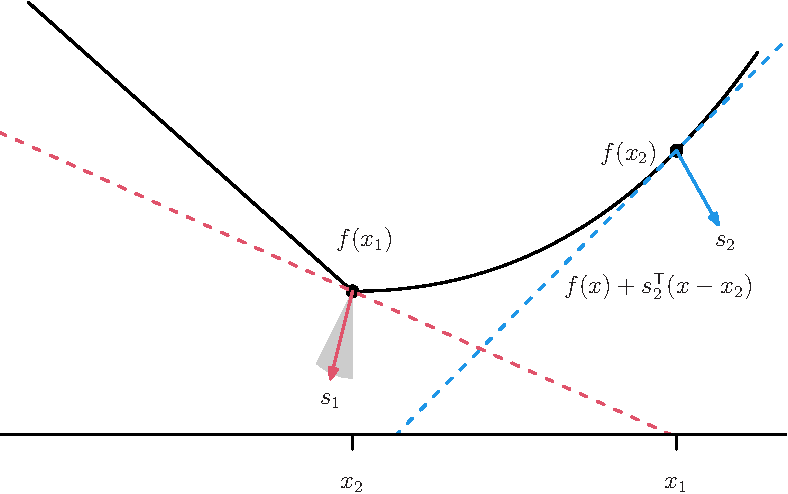
\includegraphics[width=0.7\textwidth]{fig/subgradient.pdf}
\caption{Two example subgradients $s_1$ and $s_2$ of a function $f$ at two
  points $x_1$ and $x_2$, respectively. Each $s_i$ defines a linear map 
  that passes through $x_i$ and lies below $f$ everywhere (that is, it defines a
  supporting hyperplane to $\epi(f)$ at $x_i$, whose normal is $(s_i,-1)$). At
  $x_2$, $f$ is differentiable, and $s_2 = \nabla f(x_2)$ is the only
  subgradient; at $x_1$ there are many possible subgradients (as illustrated
  by the gray wedge).}
\label{fig:subgradient}
\end{figure}

\index{subdifferential}
The set of all subgradients of $f$ at $x$ is called its \emph{subdifferential}
at $x$, which we denote by $\partial f(x)$. One can check that $\partial f(x)$
is always a closed convex set (regardless of whether $f$ itself is convex).  If
$\partial f(x)$ is nonempty, then $f$ is said to be \emph{subdifferentiable} at
$x$. Sometimes we will use a subscript on the subdifferential operator to
emphasize the variable under consideration. For example, when $f$ is a function 
of a block variable $(x,y)$, we use $\partial_x f(x,y)$ for the subdifferential
of the function $f(\cdot, y)$ at $x$, with its second argument fixed at $y$.

The notions defined above are apparently general, in that we have not assumed 
convexity of the function $f$ in question. However, as we will see in our 
discussion of some of the basic properties of subgradients and subdifferentials
below, these concepts are in fact intimately tied to convexity.   

\paragraph{Existence of subgradients.}

By rearranging the inequality in \eqref{eq:subgradient}, one finds that 
\[
s \in \partial f(x) \iff \text{$\epi(f)$ has a supporting hyperplane at
  $(x, f(x))$ with normal vector $(s, -1)$.}
\]
We see that the existence of a subgradient of $f$ at a point is linked to the
existence of a supporting hyperplane at a certain point of $\epi(f)$. Given the
existence of supporting hyperplanes for convex sets, it is reasonable to expect
that subgradients also exist in some generality for convex functions (whose
epigraphs are convex). The next result gives the details.

\index{subgradient!existence}
\begin{Theorem}
\label{thm:subgradient_existence}
A convex function $f$ is subdifferentiable at every point in $\relint(\dom(f))$,
the relative interior of its effective domain. In particular, this means that a
convex function that is finite on all of $\R^d$ is subdifferentiable at every
point.   

\setlength{\parindent}{\normalparindent}
Conversely, if $f : \R^d \to (-\infty, \infty]$ is closed, the set $\dom(f)$ is
convex, and $f$ is subdifferentiable on $\relint(\dom(f))$, then $f$ must be
convex.          
\end{Theorem}

As alluded to earlier, the first part of Theorem
\ref{thm:subgradient_existence}, on the existence of subgradients for a convex
function, is based on applying the supporting hyperplane theorem to the epigraph
representation of subgradients; the proof is outlined in Exercise
\ref{ex:subgradient_existence}. The second part, on subdifferentiability
implying convexity, is based on a converse supporting hyperplane theorem; see
Exercises \ref{ex:converse_supporting_hyperplane} and
\ref{ex:subdifferentiability_implies_convexity}. 

\paragraph{Uniqueness of subgradients.}

The subgradient of $f$ at a given point $x \in \dom(f)$ need not be unique, that
is, the subdifferential $\partial f(x)$ (when nonempty) need not be a
singleton. So, when it is unique at $x$, what can we say about $f$ at $x$,
vis-a-vis differentiability? The answer is nothing, in general (Exercise
\ref{ex:subgradient_nonuniqueness}). However, for convex $f$, the subgradient of
$f$ is unique at $x$ if and only it is differentiable at $x$. This result is
stated formally next; Exercise \ref{ex:subgradient_uniqueness} walks through its
proof. 

\index{subgradient!uniqueness}
\begin{Theorem}
\label{thm:subgradient_uniqueness}
Let $f$ be a convex function. If $f$ is differentiable at a point $x \in
\dom(f)$, then it has a unique subgradient $s = \nabla f(x)$ at $x$. Conversely,
if $f$ has a unique subgradient $s$ at $x$, then it is differentiable at $x$ and
$\nabla f(x) = s$.  
\end{Theorem} 

% Theorem 25.1 in Rockafellar (1970)

An interesting practical consequence of the last result is that we can infer the
differentiability of a convex function at a point (based on it having only one
subgradient), when it may be otherwise hard to see this from first
principles. This is the case in several of the next examples.

\medskip

\begin{Example}
\label{xa:norm_subgradients}
The following are examples of subgradients of common norms. For the first two
examples, the claims can be checked directly using the definition. The others
follow from Property \parref{par:subgradient_supremum} and the dual
representation of the norm in question. % and for these we refer to exercises
% that trace out the details.      

\begin{enumerate}[label=\alph*., ref=\alph*]
\item For $f(x) = |x|$, we have 
  \[
  \partial f(x) = \begin{cases}
  \{+1\} & x > 0 \\
  \{-1\} & x < 0 \\
  [-1,1] & x = 0
  \end{cases}.
  \]

\item \parlab{xa:l1_norm_subgradients}
  For $f(x) = \|x\|_1$, subgradients $s \in \partial f(x)$ are points of the
  form:  
  \index{l1 norm@$\ell_1$ norm!subgradients}
  \[
  s_i \in \begin{cases}
  \{+1\} & x_i > 0 \\
  \{-1\} & x_i < 0 \\
  [-1,1] & x_i = 0
  \end{cases}, \quad i=1,\ldots,d.
  \]
  We see that the $\ell_1$ norm is differentiable at each point $x$ that does
  not lie on any of the coordinate axes ($x_i \not=0$ for all 
  $i=1,\ldots,d$).  

\item \parlab{xa:lp_norm_subgradients}
  For $f(x) = \|x\|_p$, and $1 < p < \infty$, let $1 < q < \infty$ be such that
  $1/p + 1/q = 1$. Then for $x \not= 0$, we have (Exercise
  \ref{ex:lp_norm_subgradients} part a):   
  \index{lp norm@$\ell_p$ norm!subgradients}
  \[
  s_i = \sign(x_i) |x_i|^{p/q} \cdot \|x\|_p^{-p/q}, \quad i=1,\ldots,d 
  \]
  as the unique subgradient in $\partial f(x)$, and for $x=0$, we have $\partial
  f(0) = \{s : \|s\|_q \leq 1\}$. We see that the $\ell_p$ norm, $1 < p <
  \infty$, is differentiable at any $x \not= 0$. Note that for $p=2$ in
  particular, we have:
  \[
  \partial f(x) = \begin{cases}
  \{x / \|x\|_2\} & x \not= 0 \\
  \{s : \|s\|_2 \leq 1\} & x = 0
  \end{cases}.
  \]

\item \parlab{xa:linf_norm_subgradients} 
  For $f(x) = \|x\|_\infty$, subgradients $s \in \partial f(x)$ are points of
  the form (Exercise \ref{ex:lp_norm_subgradients} part b): 
  \index{linf norm@$\ell_\infty$ norm!subgradients}
  \[
  s_i \in \begin{cases}
  [0,1] & \hphantom{-} x_i = \|x\|_\infty \\   
  [-1,0] & -x_i = \|x\|_\infty \\
  \{0\} & \, |x_i| < \|x\|_\infty 
  \end{cases}, \quad i=1,\ldots,d,
  \]
  where $\|s\|_1 \leq 1$. We see that the $\ell_\infty$ norm is differentiable
  at any $x$ that has a unique maximum absolute coordinate.  

\item \parlab{xa:operator_norm_subgradients} 
  For $f(X) = \|X\|_{\op}$, the operator norm, we have (Exercise
  \ref{ex:operator_norm_subgradients}):  
  \index{operator norm!subgradients}
  \[
  \partial f(X) = \conv \{ u v^\T : \|u\|_2 \leq 1, \, \|v\|_2 \leq 1, \, u^\T X
  v =  \|X\|_{\op} \}.  
  \]
  In other words, subgradients are given by convex combinations of outer 
  products of top left and right singular vectors of $X$. If the top singular
  value of $X$ has multiplicity one, then this outer product is unique (there is
  only one top left and right singular vector, up to sign flips), and the
  operator norm is differentiable at $X$ with derivative $u v^\T$.         

\item \parlab{xa:trace_norm_subgradients}  
  For $f(X) = \|X\|_{\tr}$, the trace norm, letting $X = U \Sigma V^\T$ denote
  the SVD of $X$, we have (Exercise \ref{ex:trace_norm_subgradients}):   
  \index{trace norm!subgradients}
  \[
  \partial f(X) = \{ U V^\T + W: \|W\|_{\op} \leq 1, \, U^\T W = 0, \, W V = 0
  \}. 
  \]
  In other words, subgradients are given by adding to $U V^\T$ a matrix $W$ of
  at most unit operator norm that is orthogonal to the columns of $U$ and the
  rows of $V$. If $X$ has full column rank or full row rank ($X^\T X$ or $X
  X^\T$ is invertible), then only $W=0$ satisfies these constraints, and the
  trace norm is differentiable at $X$ with derivative $U V^\T$.    
\end{enumerate}
\end{Example}

\section{Subgradient calculus}

We describe rules that will be helpful in the calculation of subgradients. 

%(We note the similarity in functional operations covered here to those covered
%in Chapter \ref{sec:operations_preserving_convexity}.)  

\paragraph{Scaling.}

For any function $f$, $x \in \dom(f)$, and $a>0$, it holds that $(\partial a
f)(x) = a \partial f(x)$. This is also trivially valid for $a=0$, provided that
$\partial f(x) \not= \emptyset$.  

\paragraph{Sum.}
\parlab{par:subgradient_sum}

For any functions $f_1,\ldots,f_n$, their sum $F = f_1+\cdots+f_n$ satisfies,
for any $x \in \dom(F)$,  
\[
\partial F(x) \supseteq \partial f_1(x) + \cdots + \partial f_n(x),  
\]
where on the right we interpret $U + V = \{u + v : u \in U, \, v \in V\}$, the
set sum (Minkowski sum) of $U,V$. Moreover, if $f_1,\ldots,f_n$ are convex,
and $\cap_{i=1}^n \relint(\dom(f_i)) \not= \emptyset$, then for any $x \in
\dom(F)$,   
\[
\partial F(x) = \partial f_1(x) + \cdots + \partial f_n(x).
\]

% Theorem 23.8 in Rockafellar (1970)

\paragraph{Partial supremum.}
\parlab{par:subgradient_supremum}

Let $f$ be a function acting on a block variable $(x,z)$. If $f(\cdot,z)$ is
convex for each $z \in Z$, then the partial supremum \smash{$F = \sup_{z \in Z}
  f(\cdot,z)$} satisfies, for any $x \in \dom(F)$,
\index{partial supremum!subgradients}
\[
\partial F(x) \supseteq \closure\left( \conv\Bigg( \bigcup_{z \in \bar{Z}(x)} 
  \partial_x f(x, z) \Bigg)\right),  
\]
where \smash{$\bar{Z}(x) = \{z \in Z : f(x,z) = F(x)\}$}, the set of points at
which the supremum at $x$ is achieved. In other words, for any $z$ such that
$f(x,z)$ achieves the supremum, the subgradients of the function $f(\cdot, z)$
at $x$ are subgradients of $F$ at $x$, along with limits of convex combinations
of them. Moreover, if $\relint(\dom(F)) \not= \emptyset$, $Z$ is compact, $f$ is
continuous on $\relint(\dom(F)) \times Z$, and $f(\cdot,z)$ is \emph{closed}
and convex for each $z \in Z$, then         
\begin{equation}
\label{eq:danskin_bertsekas}
\partial F(x) = \conv\Bigg( \bigcup_{z  \in \bar{Z}(x)} \partial_x f(x, z)
\Bigg), 
\end{equation}
a result known as the \emph{Danskin-Bertsekas theorem}.  An important special
case corresponds to a finite set $Z$: if $f_i$, $i=1,\ldots,k$ are closed and
convex, then their pointwise maximum \smash{$F = \max_{i=1,\ldots,k} \, f_i$}   
satisfies \smash{$\partial F(x) =  \conv(\cup_{i : f_i(x) = F(x)} \, \partial
  f_i(x))$}, for any $x \in \dom(F)$.

\paragraph{Partial infimum.}
\parlab{par:subgradient_infimum}

Let $f$ be a function acting on a block variable $(x,z)$. If $f$ is convex and
$Z$ is a convex set, then the partial infimum \smash{$F = \inf_{z \in Z}
  f(\cdot,z)$} satisfies, for any $x \in \dom(F)$ such that $F(x) > -\infty$,  
where we now denote \smash{$\bar{Z}(x) = \{z \in Z : f(x,z) = F(z)\}$}, 
\index{partial infimum!subgradients}
\[
\partial F(x) \supseteq \closure\left( \conv\Bigg( \bigcup_{z \in \bar{Z}(x)} 
\{ s : (s, 0) \in \partial f(x, z) \} \Bigg)\right),  
\]

\paragraph{Linear composition.}
\parlab{par:subgradient_linear}

Let $f : \R^k \to (-\infty, \infty]$ be convex, and let $A \in \R^{k \times d}$,
$b \in \R^d$. Then the function $F$ defined as $F(x) = f(Ax+b)$ satisfies, for 
any $x \in \dom(F)$, 
\[
\partial F(x) \supseteq A^\T \partial f(Ax + b).
\]
Moreover, if $(\col(A) + b) \cap \relint(\dom(f)) \not= \emptyset$, then for any  
$x \in \dom(F)$,  
\[
\partial F(x) = A^\T \partial f(Ax + b).
\]

% Theorem 23.9 in Rockafellar (1970)

\paragraph{General composition.}
\parlab{par:subgradient_composition}

Let $f : \R^k \to (-\infty, \infty]$, $g : \R^d \to \R^k$, and denote their
composition by $F = f \circ g$, that is, $F(x) = f(g(x))$. If $f$ is convex and
nondecreasing in each argument, and each component function $g_i$,
$i=1,\ldots,k$ is convex, then  
\index{composition!subgradients}
\[
\partial F(x) \supseteq \{ r_1 s_1 + \cdots + r_k s_k : r = (r_1, \ldots, r_k)
\in \partial f(g(x)), \, s_i \in \partial g_i(x), \, i=1,\ldots,k \big\}.
\]
Note that the conditions here are no less general than those in Property
\parref{par:function_composition}, on the convexity of a composition; see
Exercise \ref{ex:function_composition} part b.

\medskip

\begin{Example}
The following examples can be checked using subgradient calculus rules.

\begin{enumerate}[label=\alph*.]
\item For $f(x) = h_C(X)$, the support function \eqref{eq:support_function} of a 
  compact set $C$, we have 
  \index{support function!subgradients}
  \[
  \partial h_C(x) = \bigg\{ y : y^\T x = \sup_{z \in C} \, z^\T x \bigg\},
  \]
  A norm $\|\cdot\|$ is in fact a support function, corresponding to the set
  $C = \{x : \|x\|_* \leq 1\}$. Here $\|\cdot\|_*$ is itself another norm that
  we call the dual norm of $\|\cdot\|$, and thus $C$ can be called the dual norm
  unit ball. The connection between $\|\cdot\|$ and $\|\cdot\|_*$ is detailed
  later, in Chapter \ref{sec:dual_norms}, when we cover duality; for now we
  simply observe that we can write  
  \index{dual norm}  
  \index{norm!ball}
  \begin{equation}
  \label{eq:norm_dual}
  \|x\| = \sup_{\|z\|_* \leq 1} \, z^\T x,
  \end{equation}
  and therefore by the Danskin-Bertsekas theorem \eqref{eq:danskin_bertsekas}, 
  \index{norm!subgradients}
  \begin{equation}
  \label{eq:norm_subgradients}
  \partial \|x\| = \{ y : \|y\|_* \leq 1, \, y^\T x = \|x\| \}.
  \end{equation}
  This can be used as a starting point to establish the results on subgradients
  of specific norms given in Example \ref{xa:norm_subgradients} (Exercises   
  \ref{ex:lp_norm_subgradients}--\ref{ex:trace_norm_subgradients}). 

\item For $f(x) = \|Ax\|$, where $A \in \R^{k \times d}$ and $\|\cdot\|$ is a
  norm, we have
  \[
  \partial f(x) = \{ A^\T y :  \|y\|_* \leq 1, \, y^\T A x = \|Ax\| \}.
  \]
  Here $\|\cdot\|_*$ the dual norm of $\|\cdot\|$, as in the last example.

\item For $f(x) = \inf_{z \in C} \|x - z\|_2$, where $C$ is closed and
  convex, suppose $x \notin C$. Letting $P_C$ denote the (Euclidean)
  projection operator onto $C$, which satisfies $\|x - P_C(x)\|_2 = f(x)$, we
  have  
  \begin{equation}
  \label{eq:set_distance_subgradients}
  \partial f(x) = \bigg\{ \frac{x - P_C(x)}{\|x - P_C(x)\|_2} \bigg\}. 
  \end{equation}
\end{enumerate}
\end{Example}

\section{Subgradient optimality condition}
\label{sec:subgradient_optimality}

Subgradients have an important connection to the minimization of a function. The 
following can be checked directly from the definition of a subgradient in
\eqref{eq:subgradient}: $f(x) \leq f(y)$ for all $y$ if and only if
\index{subgradient!optimality condition}
\begin{equation}
\label{eq:subgradient_optimality}
0 \in \partial f(x). 
\end{equation}
This is called the \emph{subgradient optimality condition} for $f$. Note that it 
generalizes the more familiar zero-gradient condition \eqref{eq:zero_gradient}
for differentiable convex $f$, since for differentiable convex $f$, the only
subgradient at $x$ is the gradient $\nabla f(x)$ (Theorem
\ref{thm:subgradient_uniqueness}). We will soon find the subgradient optimality
condition \eqref{eq:subgradient_optimality} very useful, when we discuss
proximal operators in the next chapter.  

This can be extended to an optimality condition for the constrained problem,
\[
\minimize_x \quad f(x) \quad \st \quad x \in C.
\]
for a convex function $f$ and convex set $C$, where $\relint(\dom(f)) \cap
\relint(C) \not= \emptyset$.  We rewrite this problem in characteristic form    
\[
\minimize_x \quad f(x) + I_C(x),
\]
and observe that $x \in C$ is a solution if and only if zero is a subgradient
of the criterion at $x$, which (using convexity of $f$ and $I_C$, and the
subgradient rule for a sum in Property \parref{par:subgradient_sum}), can be
written as $0 \in \partial f(x) + \partial I_C(x)$, that is,
\[ 
-s \in I_C(x), \quad \text{for some $s \in \partial f(x)$}. 
\]
It remains to compute the subdifferential of $I_C$, the characteristic function
of the convex set $C$. A straightforward calculation reveals     
\index{characteristic function!subgradients} 
\index{normal cone}
\[
\partial I_C(x) = \cN_C(x) = \{ s : s^\T x \geq s^\T y, \, \text{for all $y \in
  C$}\}. 
\]
the normal cone to $C$ at $x$, and the second-to-last display, the (necessary 
and sufficient) subgradient optimality condition for a constrained convex
problem, becomes      
\begin{equation}
\label{eq:subgradient_optimality_constrained}
s^\T (y - x) \geq 0, \quad \text{for some $s \in \partial f(x)$ and all $y \in 
  C$},
\end{equation}
which nicely generalizes the first-order optimality condition
\eqref{eq:first_order_optimality} covered in Chapter
\ref{sec:properties_convex_problems}. 

\section{Subgradient monotonicity*}

The subdifferential of a function $f$ is a \emph{monotone operator}, which means
that it satisfies 
\index{subgradient!monotonicity}
\begin{equation}
\label{eq:subgradient_monotonicity}
(s_x - s_y)^\T (x - y) \geq 0, \quad \text{for all $x,y \in \dom(f)$, and 
  $s_x \in \partial f(x)$, $s_y \in \partial f(y)$}.    
\end{equation}
For given $x,y$, the inequality can be seen by simply adding together the two
conditions defining the subgradients, $f(y) \geq f(x) + s_x^\T (y-x)$ and $f(x)
\geq f(y) + s_y^\T (x-y)$, and rearranging. Note that this generalizes the
monotone gradient condition \eqref{eq:gradient_monotonicity} satisfied by a
differentiable convex function. 

It is natural to ask whether there is a converse to the subgradient monotonicity
condition. For gradients, recall, there is a converse result: if $f$ is
differentiable, and $(\nabla f(x) - \nabla (y))^\T (x-y) \geq 0$ for all $x,y$,
then $f$ is convex (Exercise \ref{ex:gradient_monotonicity}). However, for
subgradients we will need to be careful at the outset, in even just posing the
question precisely. For example, if $\partial f(x) = \emptyset$ for all $x$, as
would be the case for (say) differentiable and strictly concave $f$, then
\eqref{eq:subgradient_monotonicity} is vacuously true, but clearly $f$ is not
convex. On the other hand, if we assumed that subgradients exist on
$\relint(\dom(f))$, then $f$ would already be convex (provided $f$ is closed;
recall Theorem \ref{thm:subgradient_existence}).

A way to pose the converse question precisely is as follows. Given a set-valued
operator $T$, with $T(x) \subseteq \R^d$ for each $x \in \R^d$ (and possibly
$T(x) = \emptyset$ for some $x$), if 
\index{monotone operator}
\begin{equation}
\label{eq:T_monotonicity}
(s_x - s_y)^\T (x - y) \geq 0, \quad \text{for all $x,y$, and $s_x \in T(x)$,
  $s_y \in T(y)$}, 
\end{equation}
then does there exist a convex function $f$ for which $T \subseteq \partial f$?
This is a kind of \emph{embedding} problem: we are asking whether the graph of
$T$ embeds into the graph of the subdifferential $\partial f$ of some convex
function $f$; or equivalently, given a set of pairs $\{ (x_i, s_i) : i \in I \}$
(the graph of $T$, where $I$ is possibly infinite), we are seeking a convex
function $f$ that satisfies the relations 
\[
f(y) \geq f(x_i) + s_i^\T (y-x_i), \quad i \in I.
\] 

Interestingly, monotonicity of $T$, as in \eqref{eq:T_monotonicity}, is not
enough, but a suitable generalization of this condition is. To motivate this,
let $(x_i, s_i)$, $i=1,\ldots,n$ denote any $n$ points in the graph of $\partial
f$; that is, satisfying $s_i \in \partial f(x_i)$, $i=1,\ldots,n$. Writing
$x_{n+1}=x_1$ for convenience, adding together the $n$ subgradient inequalities  
\[
f(x_{i+1}) \geq f(x_i) \geq s_i^\T (x_{i+1} - x_i), \quad i=1,\ldots,n,
\]
and rearranging, gives 
\begin{equation}
\label{eq:T_monotonicity_n}
s_1^\T (x_2 - x_1) + s_2^\T (x_3 - x_2) + \cdots + s_{n-1}^\T (x_n -
x_{n-1}) + s_n^\T (x_1 - x_n) \leq 0.
\end{equation}
An operator $T$ that satisfies \eqref{eq:T_monotonicity_n} for all $n \geq 1$
and all $(x_i, s_i)$, $i=1,\ldots,n$ in its graph is said to be \emph{cyclically
monotone}. The argument just given shows that $\partial f$ is itself cyclically
monotone.
\index{monotone operator!cyclical}

The next result, which we call \emph{Rockafellar's embedding theorem}, gives a
complete characterization of subgradients and monotonicity.  

\index{Rockafellar's embedding theorem}
\index{monotone operator!maximal}
\begin{Theorem}
\label{thm:rockafellar_embedding}
Let $T$ be a set-valued operator, where $T(x) \subseteq \R^d$ for $x \in
\R^d$. There exists a convex function $f$ with $T \subseteq \partial f$ (which
means that $T(x) \subseteq \partial f(x)$ for all $x \in \R^d$) if and only if
$T$ is cyclically monotone. 

\setlength{\parindent}{\normalparindent}
Moreover, there exists a closed convex function with $T = \partial f$ if and
only if $T$ is maximal cyclically monotone (where maximal means that there is no
other cyclically monotone map $T'$ with $T \subseteq T'$). Finally, when it
exists, the solution $f$ (to the equation $T = \partial f$) is unique up to an
arbitrary additive constant.
\end{Theorem}

% Rockafellar (1966)

Note that the ``only if'' direction for the containment result $T \subseteq
\partial f$ in Theorem \ref{thm:rockafellar_embedding} was already established
in the motivating discussion before the theorem statement. For other parts of
the proof of Theorem \ref{thm:rockafellar_embedding}, see Exercise
\ref{ex:rockafellar_embedding}.

\section{Subgradients and growth*}

An important use of the monotonicity characterization
\eqref{eq:gradient_monotonicity} for the convexity of a differentiable function
was that it played a key role in the proofs of Theorems
\ref{thm:lipschitz_smoothness} and \ref{thm:strong_convexity}. These were
theorems about equivalent growth conditions, for smooth functions. With
subgradients in place of gradients, the next result essentially generalizes
Theorem \ref{thm:strong_convexity}. 

\index{strong convexity}
\begin{Theorem}
\label{thm:strong_convexity_nonsmooth}
For closed convex $f : \R^d \to (-\infty, \infty]$ and $m>0$, consider the
statements:     
\begin{enumerate}[label=(\roman*)]
\item $\|s_x - s_y\|_2 \geq m \|x-y\|_2$, for all $x,y \in \dom(f)$ and 
  $s_x \in \partial f(x)$, $s_y \in \partial f(y)$;  
\item the function $f_m$ is convex, where $f_m(x) = f(x) - \frac{m}{2}
  \|x\|_2^2$;    
\item $f(y) \geq f(x) + s_x^\T (y-x) + \frac{m}{2} \|y-x\|_2^2$, for all $x,y
  \in \dom(f)$ and $s_x \in \partial f(x)$; 
\item $(s_x - s_y)^\T (x - y) \geq m\|x-y\|_2^2$, for all $x,y \in \dom(f)$ and
  $s_x \in \partial f(x)$, $s_y \in \partial f(y)$.  
\end{enumerate}
Then the following relations hold: 
\[
\text{(i)} \impliedby \text{(ii)} \iff \text{(iii)} \iff \text{(iv)}.
\]
\end{Theorem}

The proof of Theorem \ref{thm:strong_convexity_nonsmooth} is outlined in
Exercise \ref{ex:strong_convexity_nonsmooth}, divided in two main parts. The
first part shows that $\text{(ii)} \iff \text{(iii)} \implies \text{(iv)}
\implies \text{(i)}$, using arguments entirely analogous to those used for
Theorem \ref{thm:strong_convexity} (Exercise \ref{ex:lipschitz_smoothness}). The
second part proves $\text{(iv)} \implies \text{(ii)}$, using Rockafellar's
embedding theorem, and a projection argument that reduces consideration to
set-valued operators on $\R$ (where monotone and cyclically monotone operators
coincide). An alternative proof for $\text{(iv)} \implies \text{(ii)}$ can be
given using generalized subgradients; see the chapter notes for more details.

It is worth noting that an important consequence of Theorem
\ref{thm:strong_convexity_nonsmooth} is that it establishes strongly convex
functions are coercive. See Exercise \ref{ex:strong_convexity_coercive}.

Next we give one more simple but important growth result, on the boundedness of
subgradients over compact sets. We remark that part (ii) of the next theorem in
fact establishes that a convex function is locally Lipschitz, as claimed in part
(iii) of Theorem \ref{thm:smoothness_properties}.  

\index{subgradient!boundedness}
\index{Lipschitz continuity}
\begin{Theorem}
\label{thm:subgradient_boundedness}
Let $f$ be a convex function, and let $C \subseteq \interior(\dom(f))$ be 
compact. Then:
\begin{enumerate}[label=(\roman*)]
\item $\cup_{x \in C} \, \partial f(x)$ is nonempty and bounded;  
\item $f$ is Lipschitz continuous on $C$, meaning (recall)
  \[
  |f(x) - f(y)| \leq L \|x-y\|_2, \quad \text{for all $x,y \in C$},
  \]
  with Lipschitz constant \smash{$L = \sup_{s \in \cup_{x \in C} \partial f(x)}
    \|s\|_2$}. 
\end{enumerate}
Further, as a converse to (i), the condition $x \in \interior(\dom(f))$ is also 
necessary for $\partial f(x)$ to be nonempty and bounded.   
\end{Theorem}

% For example, Proposition 5.4.2 in Bertsekas (2009) for (i) and (ii), and
% Theorem 23.4 in Rockafellar (1970) for the last part

% Note: the last statement shows we cannot relax \interior(\dom(f)) to
% \relint(\dom(f)) here! Outside of \interior(\dom(f)), the subdifferential is
% not bounded. This in particular also means that we cannot relax
% \interior(\dom(f)) to \relint(\dom(f)) in statements (ii)--(iv) of Theorem  
% \ref{thm:smoothness_properties}, or at least doing so seems nontrivial. 

\section{Subgradients and geometry*}

Subgradients possess a deep connection to convex geometry. Recall based on the
discussion before and after Theorem \ref{thm:subgradient_existence} that their
existence is tied to the fact that a subgradient of a function defines a normal
vector to its epigraph. A related interpretation is as follows: if $s \in
\partial f(x)$, then we observe straight from the definition
\eqref{eq:subgradient} that
\[
f(y) \leq f(x) \implies s^\T x \geq s^\T y.
\]
In other words, $s$ defines the normal to a supporting hyperplane of a sublevel
set $\{y : f(y) \leq f(x)\}$ at $x$. As the normal cone to $\{y : f(y) \leq
f(x)\}$ at $x$ is, by definition, the collection of all such normal vectors, we
can also write this conclusion as   
\[
\partial f(x) \subseteq \cN_{\{y : f(y) \leq f(x)\}}(x).
\]
Interestingly, as the next result shows, the subgradients at $x$ not only lie in
the normal cone to the sublevel set at $x$, they also generate it. 

\index{normal cone}
\begin{Theorem}
\label{thm:subgradient_normal}
Let $f$ be a convex function, and $x \in \relint(\dom(f))$ be a point at which
$f$ does not attain its infimum. Then 
\[
\cN_{\{y : f(y) \leq f(x)\}}(x) = \cone\big(\partial f(x)\big).
\]
\end{Theorem}

% For example, Theorem 23.7 in Rockafellar (1970). Removing the cl() because the
% subdifferential is closed convex bounded and does not contain the origin, so
% its convex hull should be closed. As in Corollary 9.6.1 of Rockafellar (1970)

Just like the subgradient optimality condition \eqref{eq:subgradient_optimality}
generalizes the zero-gradient condition \eqref{eq:zero_gradient} from classical
smooth analysis, we can view Theorem \ref{thm:subgradient_normal} as a
generalization of the classical result that the gradient vector $\nabla f$ lies 
orthogonal to tangent planes of level sets a smooth function $f$. See Figure
\ref{fig:subgradient_normal} for an illustration. 

\begin{figure}[tb]
\centering
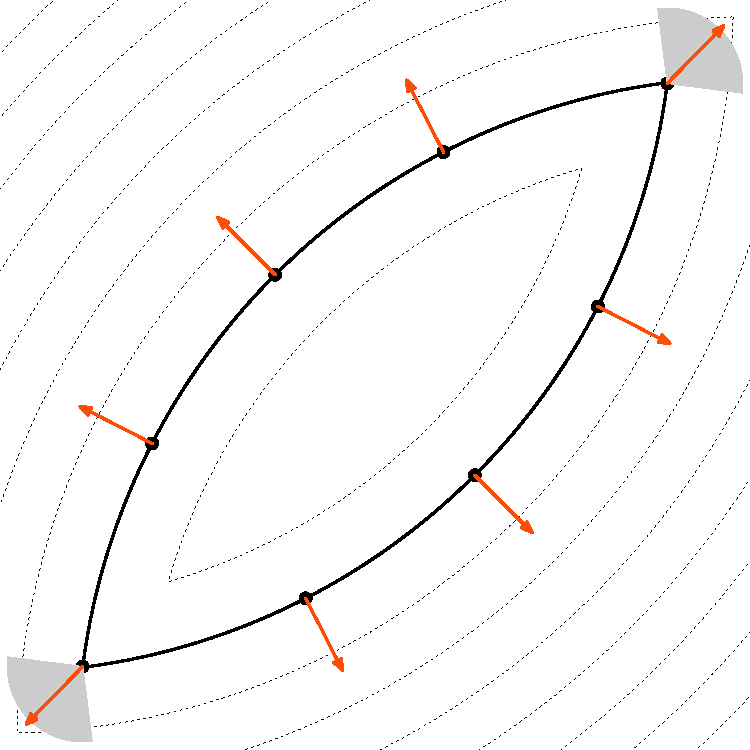
\includegraphics[width=0.525\textwidth]{fig/subgradient_normal.pdf}
\caption{Contours of a convex function $f$, with a particular level set of
  interest highlighted in solid black. At various points $x$ along the level
  set, subgradients of $f$ at $x$ are drawn, represented as normal vectors
  emanating from the level set at $x$. At two points along the level set, in the
  bottom left and top right, $f$ is not differentiable, and the subdifferentials
  are represented by gray wedges.}        
\label{fig:subgradient_normal}
\end{figure}

\index{subgradient!categorization}
Lastly, we discuss a categorization of points of subdifferentiability of $f$,
and we show how the geometric perspective provided in Theorem
\ref{thm:subgradient_normal} leads to an interesting conclusion about the number 
of points lying in the ``least smooth'' category, along any slice through the
graph of a convex function $f$. The categorization is as follows: when $k =
\dm(\spa(\partial f(x)))$, the dimension of the linear span $\partial f(x)$, we
say that $x$ is \emph{category $k$} point in the subdifferential $\partial
f(x)$. Thus, for convex $f$, at a point $x$ where $f$ does not attain its 
infimum: 
\begin{itemize}
\item $x$ is category 0 $\iff$ $f$ not subdifferentiable at $x$;
\item $x$ is category 1 $\iff$ $f$ is differentiable at $x$;
\item $x$ is category 2 $\iff$ $f$ has two linearly independent subgradients at 
  $x$, say $s_1$ and $s_2$, where $\spa\{s_1, s_2\} = \partial f(x)$; 
\item and so on, up through category $d$, where $\dom(f) \subseteq \R^d$. 
\end{itemize}
Points in category 1 can be thought of as the ``most smooth'', and points in
category $d$ as the ``least smooth'' (among categories 1 through $d$, excluding
0)---for $x$ in category $d$, the normal cone to the sublevel set $\{y : f(y)
\leq f(x)\}$ at $x$ is $d$-dimensional, which means the sublevel set looks
``pointy'' at $x$, like a vertex on a polyhedron, or the bottom left and top
right points along the level set drawn in Figure \ref{fig:subgradient_normal}. 

We already know from Theorem \ref{thm:smoothness_properties} part (iii) that
categories 2 through $d$ are, altogether, ``rare'' compared to category 1: the
union of category 2 through $d$ points only make up a set of Lebesgue measure 
zero in $\interior(\dom(f))$. But in fact, we can say something much finer along
any slice through the graph of a convex function $f$: here, it turns out, $f$
can only have a \emph{countable} number of points in category $d$, the ``least
smooth'' category. 

\begin{Theorem}
\label{thm:subgradient_category_d}
Let $f$ be convex with $\dom(f) \subseteq \R^d$, and let $t \in \R$ be
arbitrary.  Then $f$ has a countable number of category $d$ subdifferentiable
points along the level set $\{x : f(x) = t\}$. 
\end{Theorem}

% For example, Proposition 11.6.2 in Berger (2004), Part I

The proof of Theorem \ref{thm:subgradient_category_d} is elementary, and relies
critically on the normal cone formulation of subgradients in Theorem
\ref{thm:subgradient_normal}. Essentially, it uses the normal cone relationship
(and convexity of the sublevel set) to argue that the interiors of 
conic hulls of category $d$ subdifferentials along the level set form a
collection of disjoint open sets in $\R^d$, and thus by classical arguments in
analysis, there can be at most a countable number of them. See Exercise
\ref{ex:subgradient_category_d}.   

\SkipTocEntry\section*{Chapter Notes}

Jean Jacques Moreau and R. Tyrrell Rockafellar are widely considered to be the
``founding fathers'' of subdifferentiability, each having worked separately to 
develop the subject in the early 1960s. To learn more, beyond what is covered in
this chapter, a classic reference (and masterful treatment) is
\cite{rockafellar1970convex} (Chapters 23--25); other nice references are 
\cite{hiriartUrruty2001fundamentals} (Chapter D) and \cite{bertsekas2009convex} 
(Chapter 5.4). The study of monotone operators is closely linked to the study of 
subgradients (and to that of proximal operators, which will be covered in the
next chapter). Two nice very books that develop this connection, from different 
perspectives (analytic versus algorithmic) are \cite{bauschke2011convex,
  ryu2022large}. 

The Danskin-Bertsekas theorem is named after the extension given in Bertsekas'
Ph.D.\ thesis \cite{bertsekas1971control} of an earlier result by Danskin
\cite{danskin1967theory}. Even more can be said about the subdifferential of a
partial supremum of convex functions; see, for example,
\cite{hantoute2008subdifferential} for a recent overview and connections to
other subgradient calculus rules. Rockafellar's embedding theorem (which is not, 
as far as we know, a commonly used name for the result stated in this chapter)
is due to \cite{rockafellar1966characterization}.

Finally, we note that generalizations of the definition of a subgradient have
been developed for nonconvex functions, notably by Francis H.\ Clarke and
Rockafellar, in the 1980s. These definitions reduce to the usual notion of a
subgradient for convex functions, and also reduce the usual notion of a gradient
for differentiable (and possibly nonconvex) functions, but apply much more
broadly. Two authoritative references, each of which covers much more than just
generalized subgradients, are \cite{clarke1990optimization,
  rockafellar2009variational}. Generalized subgradients are not only critical
tools in nonsmooth and variational analysis, they can also be useful in
\emph{convex} analysis. For example, the generalized subgradient used in
variational analysis, as defined in \cite{rockafellar2009variational}, provides 
an alternative, short proof that $\text{(iv)} \implies \text{(ii)}$ in Theorem
\ref{thm:strong_convexity_nonsmooth}; see Exercise 12.59 in
\cite{rockafellar2009variational}.   

\clearpage

\begin{xcb}{Exercises}
\begin{enumerate}[label=\thechapter.\arabic*]
\settowidth{\leftmargini}{0.00.\hskip\labelsep}
\index{supporting hyperplane theorem!converse}
\item \label{ex:converse_supporting_hyperplane}
  This exercise proves the following converse to the supporting hyperplane
  theorem: if $C$ is a closed set, $\relint(C) \not= \emptyset$, and every $x_0
  \in \relbd(C)$ has a supporting hyperplane (there exists $a\not=0$ and $b$  
  such that $a^\T x_0 = b$ and $a^\T x \leq b$ for all $x \in C$), then $C$     
  must be convex.   

  We will assume, without a loss of generality, that $C$ is full-dimensional
  ($\aff(C) = \R^d$), so its relative interior and relative boundary are its
  interior and boundary, respectively. (Note: having proved this
  full-dimensional result, to accommodate the case when $\aff(C)$ is a proper
  subspace of $\R^d$, we can reparametrize to the affine subspace, and apply the
  result just proved to conclude that the set $D$---the reparametrization of $C$
  to the affine subspace---is convex in this coordinate system, and then simply
  view $C$ as an affine image of $D$ in order to conclude that $C$ itself is
  convex.)  

  Let $H$ be the intersection of all supporting halfspaces to $C$, 
  \[
  H = \bigcap_{x_0 \in \boundary(C)} \underbrace{\{ x :  a_{x_0}^\T x \leq
    b_{x_0} \}}_{H_{x_0}}, 
  \]
  where for each $x_0 \in \boundary(C)$, we write \smash{$a_{x_0}$} and
  \smash{$b_{x_0}$} for the normal vector and offset, respectively, that define
  the supporting hyperplane to $C$ at $x_0$. Note that $H$ is convex, and that
  $C \subseteq H$.    

\begin{enumerate}[label=\alph*.]
\item Fix $y \notin C$, and let $x \in \interior(C)$. Let
  \[
  t = \sup \{ s \geq 0 : x + s (y - x) \in C \}. 
  \]
  Prove that $s \in (0,1)$. (Hint: use that $x \in \interior(C)$, and the fact
  that $C^c = \R^d \setminus C$ is open.) Prove also that $t y \in
  \boundary(C)$. (Hint: use again the fact that $C$ is closed.) 

\item By inspecting the supporting hyperplane at $x_0 = t y$, argue that since
  $x \in H_{x_0}$, we must have \smash{$y \notin H_{x_0}$}, and thus $y \notin 
  H$. 

  \smallskip
  Since $y$ was arbitrary, note that we have shown $C^c \subseteq H^c$, that is,
  $H \subseteq C$, which together with the observation $C \subseteq H$, proves
  that $C = H$ and hence that $C$ is convex. 
\end{enumerate}

\index{subgradient!existence}
\item \label{ex:subdifferentiability_implies_convexity}
  We will now prove the second part of Theorem \ref{thm:subgradient_existence},  
  using the converse supporting hyperplane theorem from Exercise
  \ref{ex:converse_supporting_hyperplane}. Let $f$ satisfy the conditions of the 
  theorem: $f : \R^d \to (-\infty, \infty]$ is closed and has a subgradient and   
  every point in $\relint(\dom(f))$, where $\dom(f)$ is convex.

\begin{enumerate}[label=\alph*.]
\item Abbreviate $S = \relint(\dom(f))$. Prove that any point $(x,t)$ on the
  relative boundary of $\epi(f)$ can be written in one of two ``types'': 
  \begin{alignat*}{2}
  &\text{type I}: \quad &&x \in S, \; t = f(x), \\
  &\text{type II}: \quad &&x \in \dom(f) \setminus S, \; t \geq f(x). 
  \end{alignat*}

\item Prove that every relative boundary point of type I has a supporting
  hyperplane. Hint: use the existence of subgradients on $S$.

\item Prove that every relative boundary point of type II has a supporting
  hyperplane. Hint: note that $x \in \boundary(\dom(f))$, and use the fact that
  $\dom(f)$ is itself convex and thus must admit a supporting hyperplane, by the 
  supporting hyperplane theorem.

\item Complete the proof by applying the converse supporting hyperplane theorem
  to $\epi(f)$. 
\end{enumerate}

\index{subgradient!uniqueness}
\item \label{ex:subgradient_nonuniqueness} 
  Give two examples of a function $f$ that has a unique subgradient at a point
  $x$ but is nondifferentiable at $x$, where in one example $f$ is discontinuous 
  at $x$, and in another continuous. Hint: by Theorem
  \ref{thm:subgradient_uniqueness}, the function $f$ here will have to be  
  nonconvex.

\item \label{ex:affine_minorant}
  Prove that a convex function $f$ is equal to the pointwise supremum of its
  affine minorants on the relative interior of its effective domain, 
  \begin{equation}
  \label{eq:affine_minorant}
  f(x) = \sup \{ g(x) : \text{$g$ is affine, and $g \leq f$} \}, \quad \text{for
    all $x \in \relint(\dom(f))$},
  \end{equation}
  where we write $g \leq f$ to mean that $g(x) \leq f(x)$ for all $x$.

  % Theorem 12.1 in Rockafellar (1970), which actually proves that for closed
  % convex f this is true on the entire domain 

\index{directional derivative}
\item \label{ex:directional_derivative}
  For a function $f$ on $\R^d$, we define its (one-sided) \emph{directional
    derivative} with respect to $v \in \R^d$ at point $x \in \dom(f)$ by the
  (one-sided) limit  
  \begin{equation}
  \label{eq:directional_derivative}
  f'(x; v) = \lim_{t \to 0^+} \frac{f(x + tv) - f(x)}{t},
  \end{equation}
  if it exists (with $\pm \infty$ limits being allowed). Note the difference
  between the usual (two-sided) directional derivative from multivariate
  calculus, as reviewed in Appendix \ref{sec:directional_derivative}. In this
  exercise, we will explore the relationship between directional derivatives and
  subgradients. We take $f$ to be convex in what follows.

\begin{enumerate}[label=\alph*.]
\item Prove that \eqref{eq:directional_derivative} always exists (again, with
  $\pm \infty$ limits being allowed). Hint: prove that $(f(x + tv) - f(x)) / t$
  is nonincreasing as $t \to 0^+$, using convexity of 
  $f$.     

\item Prove that $v \mapsto f'(x; v)$ is convex and positively homogeneous,
  where the latter means $f'(x; \alpha v) = \alpha f'(x; v)$ for all $\alpha
  \geq 0$. 

\item For $x \in \relint(\dom(f))$, prove that 
  \[
  s \in \partial f(x) \iff f'(x; v) \geq s^\T v, \; \text{for all $v$}.
  \]

\item For $x \in \relint(\dom(f))$, prove that 
  \[
  f'(x; v) = \sup_{s \in \partial f(x)} \, s^\T v.
  \]
  Hint: use the last part to establish $\geq$ in the above display. For the
  other direction, fix $x$, denote $F_x(v) = f(x; v)$, and consider Exercise
  \ref{ex:affine_minorant} applied to $F_x$. Show that, by positive homogeneity
  of $F_x$, we in fact have
  \[
  F_x(v) = \sup \{ G(v) : \text{$G$ is linear, and $G \leq F_x$} \},
  \]
  and lastly, show that $G$ linear with $G \leq F_x$ implies $G(v) = s^\T v$ for
  $s \in \partial f(x)$, to upper bound the supremum on the right-hand side
  above, completing the proof. 
\end{enumerate}

\index{subgradient!uniqueness}
\item \label{ex:subgradient_uniqueness}
  We will work through the proof of Theorem \ref{thm:subgradient_uniqueness}.  

\begin{enumerate}[label=\alph*.]
\item If $f$ is differentiable at $x$, then show $s = \nabla f(x)$ is its
  only subgradient at $x$ by using the relation in Exercise
  \ref{ex:directional_derivative} part c between subgradients and directional 
  derivatives. Hint: if $f$ is differentiable at $x$, then note that $f'(x; v) =
  \nabla f(x)^\T v$.  

\item If $s$ is the unique subgradient at $x$, then denote $F_x(v) = f(x + v) -
  f(x) - s^\T v$, and argue that $F_x$ has 0 as its unique subgradient at the 
  origin. Show that this implies    
  \[
  \lim_{v \to 0} \frac{F_x(v)}{\|v\|_2} = 0,
  \]
  which means (by definition) that $f$ is differentiable at $x$ with $\nabla
  f(x) = s$. Hint: to prove the above display, first note that for any $v$ with
  unit norm, by Exercise \ref{ex:directional_derivative} part d (which we know
  applies, because $s$ cannot be unique if $x \notin \interior(\dom(f))$, by
  % the last statement in 
  Theorem \ref{thm:subgradient_boundedness}), 
  \[
  0 = F_x'(0; v) = \lim_{t \to 0^+} \frac{F_x(tv)}{t}.
  \]
  Then use the above pointwise convergence, along with convexity of $v \mapsto
  F_x(tv)/t$, to prove that in fact $F_x(tv)/t \to 0$ as $t \to 0^+$
  \emph{uniformly} over the unit ball $\{ v : \|v\|_2 \leq 1\}$, which leads to 
  the desired conclusion.    
\end{enumerate}
 
\item \label{ex:lp_norm_subgradients}
  We establish results on the subgradients of the $\ell_p$ norm, $1 < p <
  \infty$, and the $\ell_\infty$ norm. 

\begin{enumerate}[label=\alph*.]
\index{lp norm@$\ell_p$ norm!subgradients}
\item Prove the statement in Example \parref{xa:lp_norm_subgradients} by using 
  the dual representation    
  \[
  \|x\|_p = \sup_{\|z\|_q \leq 1} \, z^\T x,
  \]
  where $1 < q < \infty$ is such that $1/p + 1/q = 1$, and applying
  \eqref{eq:norm_subgradients} (which follows from an application of the   
  Danskin-Bertsekas theorem). Hint: in H{\"o}lder's inequality,
  \[
  a^\T b \leq \|a\|_p \|b\|_q,
  \] 
  equality holds for nonzero $a,b \in \R^d$ if and only if $a_i^p/\|a\|_p^p =
  b_i^q/\|b\|_q^q$, $i=1,\ldots,d$.  
  
\index{linf norm@$\ell_\infty$ norm!subgradients}
\item Prove the statement in Example \parref{xa:linf_norm_subgradients}
  similarly, via the dual representation,   
  \[
  \|x\|_\infty = \sup_{\|z\|_1 \leq 1} \, z^\T x,
  \]
  then applying \eqref{eq:norm_subgradients}. An alternative is to observe that
  the Danskin-Bertsekas theorem (in the case where $Z$ is finite) can be applied
  directly to \smash{$\|x\|_\infty = \max_{i=1,\ldots,d} \, |x_i|$}.     
\end{enumerate}

\index{operator norm!subgradients}
\item \label{ex:operator_norm_subgradients}
  We establish the result in Example \parref{xa:operator_norm_subgradients}, on
  the subgradients of the operator norm. We use the dual representation
  \[
  \|X\|_{\op} = \sup_{\|Z\|_{\tr} \leq 1} \, \langle Z, X \rangle, 
  \]
  covered later in Chapter \ref{sec:dual_norms} (where recall we write $\langle
  Z, X \rangle = \tr(Z^\T X)$), along with \eqref{eq:norm_subgradients}.

\begin{enumerate}[label=\alph*.]
\item Prove that if \smash{$Z = \sum_{i=1}^k u_i v_i^\T$}, where $\|u_i\|_2 
  \leq 1$, $\|v_i\|_2 \leq 1$, $u_i^\T X v_i = \|X\|_{\op}$, $i=1,\ldots,k$,
  then $\|Z\|_{\tr} \leq 1$ and $\langle Z, X \rangle =  \|X\|_{\op}$.   

\item Prove the opposite direction: if $\|Z\|_{\tr} \leq 1$ and $\langle Z, X
  \rangle = \|X\|_{\op}$ then $Z$ must be of the above form (\smash{$Z =
    \sum_{i=1}^k u_i v_i^\T$}, where $\|u_i\|_2 \leq 1$, $\|v_i\|_2 \leq 1$,
  $u_i^\T X v_i = \|X\|_{\op}$, $i=1,\ldots,k$). Hint: use an SVD of $Z$, and
  consider what the conditions on $Z$ say about the factors.      
\end{enumerate}

\index{trace norm!subgradients}
\item \label{ex:trace_norm_subgradients} 
  We establish the result in Example \parref{xa:trace_norm_subgradients}, on the
  subgradients of the trace norm. We use the dual representation 
  \[
  \|X\|_{\tr} = \sup_{\|Z\|_{\op} \leq 1} \, \langle Z, X \rangle,
  \]
  covered later in Chapter \ref{sec:dual_norms} (where recall we write $\langle 
  Z, X \rangle = \tr(Z^\T X)$), along with \eqref{eq:norm_subgradients}. As in
  the example, we write $X = U \Sigma V^\T$ for an SVD of $X$. 

\begin{enumerate}[label=\alph*.]
\item Prove that if $Z = U V^\T + W$, for $\|W\|_{\op} \leq 1$, $U^\T W = 0$,
  and $W V = 0$, then $\|Z\|_{\op} \leq 1$ and $\langle Z, X \rangle =
  \|X\|_{\tr}$. Hint: use an SVD of $Z$, and consider what the conditions on $W$
  say about the factors.   

\item Prove the opposite direction: if $\|Z\|_{\op} \leq 1$ and $\langle Z, X
  \rangle = \|X\|_{\tr}$ then $Z$ must be of the above form ($Z = U V^\T + W$,  
  where $\|W\|_{\op} \leq 1$, $U^\T W = 0$, and $W V = 0$). Hint: define $W = Z
  - U V^\T$, and consider what the conditions on $Z$ say about $W$. 
\end{enumerate}

\index{composition!subgradients}
\item Prove the result in Property \parref{par:subgradient_composition}, on
  subgradients of a composition of convex functions.   

\item Let $f$ be a function of a block variable $(x,z)$, and let 
  \[
  F(x) = \E_z[ f(x,z) ] = \int f(x,z) \, dP(z),
  \]
  for a distribution $P$ over $z$. Fix any $x$, and suppose that for each $z$,
  we have $s(z) \in \partial_x f(x,z)$. Prove that $s = \E_z[s(z)] \in \partial
  F(x)$.  

\item For a convex function $f$, suppose $s \in \R^d$ is such that at a point $x
  \in \dom(f)$,
  \[
  f(y) \geq f(x) + s^\T (y-x), \quad \text{for all $y \in \dom(f)$ such that
    $\|x - y\| \leq \delta$},
  \]
  for some $\delta>0$. Prove that $s \in \partial f(x)$. Note: this, combined
  with subgradient optimality \eqref{eq:subgradient_optimality}, gives another 
  way of seeing the fundamental theorem of convex optimization, Property
  \parref{par:convex_local}: a zero subgradient locally implies a zero
  subgradient globally.   

\index{subgradient!optimality condition}
\item Prove or disprove, for the subgradient optimality condition for a
  constrained convex problem: if \eqref{eq:subgradient_optimality_constrained} 
  holds, then there can still exist another $v \in \partial f(x)$, $v \not= s$,
  such that 
  \[
  v^\T (y - x) < 0, \quad \text{for some $y \in C$}.
  \]
  In other words, one subgradient $s$ is telling us not to move away from $x$ at
  all (restricting the search directions to those keeping us in $C$), yet
  another subgradient $v$ is telling us to move in the direction of another   
  feasible point $y$.   
  % Counterexample: f with nonsmooth level sets, and constrained minimum occurs
  % at a vertex. One subgradient has a nonnegative inner product with all y - x,
  % but some subgradients can have a negative inner product with some y - x.  

\index{Rockafellar's embedding theorem}
\item \label{ex:rockafellar_embedding}
  In this exercise, we will work through the proof of Theorem
  \ref{thm:rockafellar_embedding}. 

\begin{enumerate}[label=\alph*.]
\item To show the ``if'' direction in the containment $T \subseteq \partial f$,
  fix any $x_1$ such that $s_1 \in T(x_1)$, and define 
  \[
  f(x) = \sup\bigg\{ \sum_{i=1}^{n-1} s_i^\T (x_{i+1} - x_i) + s_n^\T (x - x_n)
  : \text{$n \geq 1$, $s_i \in \partial f(x_i)$, $i=2,\ldots,n$} \bigg\}.
  \]
  Prove that $f$ is convex and $T \subseteq \partial f$.

\item To show the ``if'' direction in the equality $T = \partial f$, observe
  that if $T$ is maximal, and $T \subseteq \partial f$, then we must have $T =
  \partial f$. Prove that, additionally, $T$ is the subdifferential of a
  \emph{closed} convex function. Hint: define \smash{$g(x) = \liminf_{y \to x} 
    f(x)$}, and show that $g$ is closed with $\partial f \subseteq \partial
  g$. Then then invoke maximality.   
\end{enumerate}

\smallskip
A note on the remaining part, the ``if'' direction in the equality $T = \partial
f$ and uniqueness of the solution $f$ to $T = \partial f$, up to an additive 
constant: the arguments required for this part are more subtle. What we can say  
immediately is that, for any closed convex $f$, we have $\partial f \subseteq
\partial g$ for some convex closed $g$, where $\partial g$ is maximal cyclically
monotone; this follows from the fact that each cyclically monotone operator must
be embedded in some maximal one (using Zorn's lemma), and that this maximal one
can always be written as $\partial g$ for closed convex $g$ (by part b of this
exercise). However, to prove the next step: 
\begin{equation} 
\label{eq:embedding_equality}
\text{$f,g$ closed convex with $\partial f \subseteq \partial g$} \implies 
\text{$f = g + c$ for some constant $c$},
\end{equation} 
requires a more involved argument. We refer the reader to the proofs of Theorems
3 and 4 in \cite{rockafellar1966characterization}, which are based on
approximate subgradients and duality; see also Theorems 12.17 and 12.25 in   
\cite{rockafellar2009variational}, which take a variational approach.      

\index{monotone operator}
\index{monotone operator!cyclical}
\index{monotone operator!maximal}
\item \label{ex:cyclical_monotonicity}
  We examine some properties of cyclical monotonicity, which, recall, for a 
  set-valued operator $T$ on $\R^d$, means that it satisfies
  \eqref{eq:T_monotonicity_n} for all $n \geq 1$ and all $(x_i, s_i)$,
  $i=1,\ldots,n$ in its graph.   

\begin{enumerate}[label=\alph*.]
\item Show that an equivalent condition for $T$ to be cyclically monotone is
  \[
  \sum_{i=1}^n s_i^\T x_i \geq \sum_{i=1}^n s_{\sigma(i)}^\T x_i,
  \]
  for all $n \geq 1$, permutations $\sigma$ on $1,\ldots,n$, and $(x_i, s_i)$,
  $i=1,\ldots,n$ in the graph of $T$.  

\item Show that when $d=1$ (so that $T$ is set-valued on $\R$), 
  monotonicity \eqref{eq:T_monotonicity} is equivalent to cyclical
  monotonicity. Hint: a cyclically monotone operator is monotone. For the other
  direction, use the condition from part a, and consider the rearrangement
  inequality.        

% \item Show that when $d>1$, this equivalence is not true, by giving an example 
%   of a monotone operator that is not cyclically monotone.  
\end{enumerate}

\index{strong convexity}
\item \label{ex:strong_convexity_nonsmooth}
  In this exercise, we will work through the proof of Theorem
  \ref{thm:strong_convexity_nonsmooth}. 

\begin{enumerate}[label=\alph*.]
\item Prove that $\text{(ii)} \iff \text{(iii)}$ by using the subgradient
  characterization of convexity for $f_m$, from Theorem
  \ref{thm:subgradient_existence}. Prove that $\text{(iii)} \implies
  \text{(iv)}$ using subgradient monotonicity (applied to $f_m$), and
  $\text{(iv)} \implies \text{(i)}$ using the Cauchy-Schwarz inequality. Note
  that these arguments are analogous to those given in Exercise 
  \ref{ex:lipschitz_smoothness} for Theorem \ref{thm:strong_convexity}.   
  
\item Now we will work towards $\text{(iv)} \implies \text{(ii)}$, in steps laid
  out over the next couple of parts. First, fix any $x \in \dom(f)$, $v \in
  \R^d$, and let $g(t) = f_m(x + tv)$. Define 
  \[
  T(t) = \{ s^\T v : s \in \partial f(x+vt) - m(x+vt) \}.
  \]
  Use (iv) to argue that $T$ is monotone, in fact, cyclically monotone by
  Exercise \ref{ex:cyclical_monotonicity} part b (as $T$ set-valued in $\R$). 

\item Apply Rockafellar's embedding theorem and the closedness of $f$ to
  conclude $g$ is convex, and as $x,v$ were arbitrary, $f_m$ itself must be
  convex. Hint: by the embedding theorem, we know that $T \subseteq \partial h$
  for some closed convex function $h$. Rewrite this containment as 
  \[
  \partial g(x) \subseteq \partial h(x) + m(x+vt), \quad \text{for all $x$}.
  \]
  Now use closedness of $g$ and \eqref{eq:embedding_equality} to prove that $g$
  is convex. 
\end{enumerate}

\index{coercive function}
\item \label{ex:strong_convexity_coercive}
  Prove that a strongly convex function is coercive. Hint: use part (iii) of
  Theorem \ref{thm:strong_convexity_nonsmooth}.  

% \index{subgradient!boundedness}
% \item \label{ex:subgradient_boundedness}
%   We work through the proof of Theorem \ref{thm:subgradient_boundedness}. 

% \begin{enumerate}[label=\alph*.]
% \item To prove (i), assume for the sake of contradiction that there is an 
%   unbounded sequence 
%   \[
%   \{s_k\}_{k=1}^\infty \subseteq \bigcup_{x \in C} \, \partial f(x).
%   \]
%   Then use compactness of $C$ and continuity of $f$ over $C$ (Theorem 
%   \ref{thm:smoothness_properties} part (i)) in order to achieve a
%   contradiction.   

% \item To prove (ii), use boundedness from (i), and apply the Cauchy-Schwarz
%   inequality to the subgradient definition.
% \end{enumerate}

\item \label{ex:subgradient_category_d}
  We will prove Theorem \ref{thm:subgradient_category_d}. Let $\cX$ denote the
  set of category $d$ subdifferentiable points along the level set $\{x : f(x) =
  t\}$, and denote $U_x = \interior(\cone(\partial f(x)))$, for $x \in \cX$. 

\begin{enumerate}[label=\alph*.]
\item Prove that $U_x \not= \emptyset$, $x \in \cX$.

\item Prove that $U_x \cap U_y = \emptyset$, for each $x \not= y$. Hint: use
  convexity of $\{x : f(x) \leq t\}$, and the normal cone representation of the 
  subdifferentials, from Theorem \ref{thm:subgradient_normal}.    

\item Prove that any collection of open disjoint subsets in $\R^d$ must be 
  countable, completing the proof of Thoerem
  \ref{thm:subgradient_category_d}. Hint: use the fact that the rationals are
  dense in $\R^d$.
\end{enumerate}

\end{enumerate}
\end{xcb}
\chapter{Proximal mappings}
\label{chap:proximal_mappings}

\section{Definition and properties}

In this chapter we cover a useful concept that generalizes the notion of
(Euclidean) projection onto a given set: the \emph{proximal mapping} (also
called proximal map, or proximal operator) associated with a function $f : \R^d
\to [-\infty, \infty]$. This is a set-valued map, denoted by $\prox_f$, that
maps each $x \in \R^d$ to a subset of $\R^d$ (possibly the empty set), defined
by          
\index{proximal mapping}
\begin{equation}
\label{eq:proximal_mapping}
\prox_f(x) = \argmin_z \bigg\{ \frac{1}{2} \|x - z\|_2^2 + f(z) \bigg\}. 
\end{equation}
Here and throughout, we denote by $\argmin_{z \in S} F(z)$ the set of
minimizers of a function $F$ over a set $S$, and denote by $\argmin_z F(z)$ 
the set of minimizers of $F$ over its entire effective domain. We will abide by
the common convention that $\argmin$ returns the minimizer itself when the
latter is unique (not the set containing the minimizer).     

As mentioned, we can think of $\prox_f$ as a generalization of the projecton map
onto a set. Indeed for $f = I_C$, the characteristic function of a set $C$,  
\index{projection}
\begin{equation}
\label{eq:proximal_mapping_projection}
\prox_f(x) = P_C(x) = \argmin_{z \in C} \, \|x - z\|_2.
\end{equation}
Keeping this connection in mind will generally be helpful for developing
intuition about proximal maps because---as we will see in what follows---the  
proximal map associated with a closed convex function shares several useful
properties of projection onto a closed convex set. 

A slight variation on \eqref{eq:proximal_mapping} will be of central interest in
this chapter,  
\index{proximal mapping}
\begin{equation}
\label{eq:proximal_mapping_lambda}
\prox_{\lambda f}(x) = \argmin_z \bigg\{ \frac{1}{2\lambda} \|x - z\|_2^2 + 
f(z) \bigg\},  
\end{equation}
which is simply the proximal map associated with the scaled
function $\lambda f$ for $\lambda > 0$. An intimately related object is 
\index{Moreau envelope}
\begin{equation}
\label{eq:moreau_envelope_lambda}
f_\lambda(x) = \inf_z \bigg\{ \frac{1}{2\lambda} \|x - z\|_2^2 + f(z)
\bigg\}, 
\end{equation}
called the \emph{Moreau envelope} of $\lambda f$, which will be studied a bit
later in Chapter \ref{sec:moreau_envelope}. 

We now discuss some basic properties and interpretations of proximal
mappings. We generally assume henceforth that $f \not= \infty$ ($\dom(f) \not= 
\emptyset$) to rule out trivialities when studying proximal maps.      

\paragraph{Existence and uniqueness.}

First we discuss a case where the proximal mapping acts as a well-defined 
function, from $\R^d$ to $\R^d$. If $f$ is closed and convex, then for any
$\lambda > 0$ the function    
\[
z \mapsto \frac{1}{2\lambda} \|x - z\|_2^2 + f(z)
\]
is closed and strongly convex. For the proximal mapping
\eqref{eq:proximal_mapping_lambda} to be a function (single-valued rather than
set-valued), we need a minimizer of the function in the above display to exist
and be unique. Existence comes from Weirstrass' theorem (Theorem
\ref{thm:weierstrass}), along with the fact that strongly convex functions are
coercive (Exercise \ref{ex:strong_convexity_coercive}). Uniqueness comes from
the fact that strictly (thus strongly) convex functions have at most one
minimizer (Exercise \ref{ex:convex_solution} part d). We summarize this next. 

\index{proximal mapping!existence and uniqueness}
\begin{Theorem}
\label{thm:proximal_existence_uniqueness}
For a closed and convex function $f : \R^d \to (-\infty, \infty]$ with nonempty
domain, and for any $\lambda > 0$, the proximal map
\eqref{eq:proximal_mapping_lambda} is a well-defined function: it maps each
point in $x \in \R^d$ to a point $\prox_{\lambda f}(x) \in \R^d$.   
\end{Theorem}
\vspace{-3pt}

\paragraph{Subgradient characterization.}

For closed convex $f$, the optimization problem 
\[
\minimize_z \quad \frac{1}{2\lambda} \|x - z\|_2^2 + f(z)
\]
has a subgradient optimality condition: $0 \in (z - x) / \lambda + \partial
f(z)$, that is, $x - z \in \lambda \partial f(z)$. (Convexity is used here to
write the subdifferential of a sum as a sum of subdifferentials, by Property 
\parref{par:subgradient_sum}.) Therefore by subgradient optimality, we get $z =
\prox_{\lambda f}(x)$ if and only if 
\index{proximal mapping!subgradient characterization}
\begin{equation}
\label{eq:proximal_subgradient_characterization}
x - z \in \lambda \partial f(z),
\end{equation}
which we call the subgradient characterization of the proximal operator
associated with $\lambda f$. 

For $f = I_C$, the characteristic function of a convex set $C$, if we set (say)
$\lambda = 1$, and recall that $\partial I_C(z) = \cN_C(z)$, the normal cone to
$C$ at $z$, then we can see that
\eqref{eq:proximal_subgradient_characterization} reduces to the variational
inequality \eqref{eq:variational_inequality} for the projection $z = P_C(x)$ of
$x$ onto $C$.

\paragraph{Gradient step interpretation.}

The subgradient characterization
\eqref{eq:proximal_subgradient_characterization} leads to a nice interpretation
for \smash{$\prox_{\lambda f}(x)$} when $f$ convex and differentiable. In this
case, note that \eqref{eq:proximal_subgradient_characterization} becomes a
fixed-point equation for \smash{$z = \prox_{\lambda f}(x)$},  
\[
z = x - \lambda \nabla f(z).
\]
For small $\lambda$, it is reasonable to assume that \smash{$z = \prox_{\lambda
    f}(x)$} will be close to $x$ (as the term $\|x - z\|_2^2$ in the criterion
in \eqref{eq:proximal_mapping_lambda} will be multiplied by a large weight), so 
replacing $\nabla f(z)$ with $\nabla f(x)$ in the above fixed-point equation
gives the approximation  
\begin{equation}
\label{eq:proximal_gradient_step_approx}
\prox_{\lambda f}(x) \approx x - \lambda \nabla f(x).
\end{equation}
That is, for small $\lambda$, we can interpret \smash{$\prox_{\lambda f}(x)$} as 
performing a gradient descent step starting at $x$, with step size $\lambda$. We 
will return to this interpretation in Chapter \ref{sec:moreau_envelope}, when we
will be able to make a more precise statement involving the Moreau envelope.    

\paragraph{Resolvent of subdifferential.}

A transformation of the subgradient characterization
\eqref{eq:proximal_subgradient_characterization} yields another important  
interpretation for the proximal operator. Rearranging the right-hand side in
\eqref{eq:proximal_subgradient_characterization}, and using $I$ for the identity
map, we get
\begin{align*}
z = \prox_{\lambda f}(x) &\iff x \in (I + \lambda \partial f)(z) \\
&\iff z \in (I + \lambda \partial f)^{-1}(x).
\end{align*}
Here, we should interpret $I + \lambda \partial f$ as a set-valued map: in
general, it evaluates to $(I + \lambda \partial f)(z) = \{ z + \lambda s : s \in 
\partial f(z) \}$, and its preimage to $(I + \lambda \partial f)^{-1}(x) = \{ z
: x \in (I + \lambda \partial f)(z) \}$. Inspecting the above display
carefully, we can see that it reveals something quite interesting: the preimage in
the last line must actually be \emph{single-valued}, since there is exactly one
point \smash{$z = \prox_{\lambda  f}(x)$} that satisfies $z \in (I + \lambda
\partial f)^{-1}(x)$. This allows us to write      
\index{proximal mapping!resolvent of subdifferential}   
\begin{equation}
\label{eq:proximal_resolvent_characterization}
\prox_{\lambda f} = (I + \lambda \partial f)^{-1},
\end{equation}
where we interpret both the left- and right-hand sides in
\eqref{eq:proximal_resolvent_characterization} as single-valued mappings. This
is a representation for the proximal map in terms of what is called the 
\emph{resolvent} of the subdifferential.  

\medskip

\begin{Example}
\label{xa:proximal_mappings}
The following are examples of proximal maps of general interest in statistics
and machine learning. In each case, the stated result can be derived using the 
subgradient characterization \eqref{eq:proximal_subgradient_characterization} 
for the proximal operator.

\begin{enumerate}[label=\alph*., ref=\alph*]
\item For $f(x) = \frac{1}{2} x^\T A x + b^\T x + c$ with $A \succeq 0$, we have 
  \[
  \prox_{\lambda f}(x) = (I + \lambda A)^{-1} (x - \lambda b).
  \]

\item \parlab{xa:l1_norm_proximal_mapping} 
  For $f(x) = \|x\|_1$, we have (Exercise \ref{ex:lp_norm_proximal_mapping} part 
  a): 
  \index{l1 norm@$\ell_1$ norm!proximal mapping}
  \[
  [\prox_{\lambda f}(x)]_i = [S_\lambda(x)]_i = [x_i - \sign(x_i) \lambda]_+,
  \quad i = 1,\ldots,d.
  \]
  where recall $a_+ = \max\{a, 0\}$ gives the positive part of $a$, and we
  interpret $\sign(0) = 1$. The operator $S_\lambda$ is called (coordinatewise)
  \emph{soft-thresholding} at the level $\lambda$, equivalently   
  \index{soft-thresholding}
  \begin{equation}
  \label{eq:soft_thresholding}
  [S_\lambda(x)]_i = 
  \begin{cases}
  x_i - \lambda & \text{if $x_i > \lambda$} \\
  0 & \text{if $|x_i| \leq \lambda$} \\
  x_i + \lambda & \text{if $x_i < -\lambda$}
  \end{cases},
  \quad i = 1,\ldots,d.
  \end{equation}

\item \parlab{xa:l2_norm_proximal_mapping}  
  For $f(x) = \|x\|_2$, we have (Exercise \ref{ex:lp_norm_proximal_mapping} part
  b): 
  \[
  \prox_{\lambda f}(x) = \bigg(1 - \frac{\lambda}{\|x\|_2} \bigg)_+ x.
  \]

\item \parlab{xa:trace_norm_proximal_mapping} 
  For $f(X) = \|X\|_{\tr}$, the trace norm, and $X = U \Sigma V^\T$ denoting the
  SVD of $X$, we have (Exercise \ref{ex:matrix_norm_proximal_mapping1} part a):      
  \index{trace norm!proximal mapping}
  \[
  \prox_{\lambda f}(X) = U \diag(S_\lambda(\sigma)) V^\T.
  \]
  where $\sigma$ is the vector of singular values (the diagonal of $\Sigma$),
  $S_\lambda$ is the soft-thresholding operator defined above, and we use $A =
  \diag(a)$ to construct a diagonal matrix $A$ from a vector of diagonal
  elements $a$. The proximal operator here is typically denoted $M_\lambda$, and
  called \emph{matrix soft-thresholding}.
  \index{matrix soft-thresholding}

\item \parlab{xa:frobenius_norm_proximal_mapping}  
  For $f(X) = \|X\|_F$, the Frobenius norm, we have (Exercise
  \ref{ex:matrix_norm_proximal_mapping1} part b):    
  \index{Frobenius norm!proximal mapping}
  \[
  \prox_{\lambda f}(X) = \bigg(I - \frac{\lambda}{\|X\|_F} \bigg)_+ X,
  \] 
  where $A_+$ returns the elementwise positive part of a matrix $A$. 

\item \parlab{xa:l0_norm_proximal_mapping}   
  For $f(x) = \|x\|_0$, the $\ell_0$ norm (recall this returns the number of
  nonzero values, as in \eqref{eq:l0_norm}; it is nonconvex and \emph{not}  
  actually a norm) we have (Exercise \ref{ex:lp_norm_proximal_mapping} part c):   
  \index{l0 norm@$\ell_0$ norm!proximal mapping}
  \index{hard-thresholding}
  \[
  [\prox_{\lambda f}(x)]_i = [H_\lambda(x)]_i 
  = x_i 1\{|x_i| > \lambda\}, \quad i = 1,\ldots,d.
  \]  
  The operator $H_\lambda$ is known as (coordinatewise) \emph{hard-thresholding}
  at the level $\lambda$. 

\item \parlab{xa:rank_proximal_mapping}    
  For $f(x) = \rank(X)$ (recall this is nonconvex), and $X = U \Sigma V^\T$
  denoting the SVD of $X$, we have (Exercise
  \ref{ex:matrix_norm_proximal_mapping2} part c):  
  \[
  \prox_{\lambda f}(X) = U \diag(H_\lambda(\sigma)) V^\T,
  \]
  where $H_\lambda$ is the hard-thresholding operator as defined above.
\end{enumerate}
\end{Example}

What can we do when the proximal operator is not available in closed-form? In
some settings, fast computaton may still be possible using specialized
techniques.  

\begin{Example}
\label{xa:proximal_mappings_efficient}
The examples below highlight interesting proximal mappings that cannot be 
computed in closed-form, but can still be efficiently evaluated using
specialized  algorithms.     

\begin{enumerate}[label=\alph*., ref=\alph*]
\item Let $y_i \in \R$, $i = 1,\ldots,n$ be independent draws from an
  exponential family distribution with distinct natural parameters $\eta_i \in
  \R$, $i=1,\ldots,n$, but a common sufficient statistic $T : \R \to \R$ and
  log-partition function $\psi : \R \to \R$. The negative log likelihood 
  is       
  \[
  f(\eta) = \sum_{i=1}^n \Big( \psi(\eta_i) - T(y_i) \eta_i \Big),
  \]
  where we have dropped terms not depending on $\eta$. The associated proximal
  operator 
  \index{exponential family!proximal mapping}
  \[
  \prox_{\lambda f}(\eta) = \argmin_{u} \bigg\{ \frac{1}{2} \|\eta - u\|_2^2 +
  \lambda \sum_{i=1}^n \Big( \psi(u_i) - T(y_i) u_i \Big) \bigg\}
  \]
  is not generally available in closed-form, but is efficiently computable for
  differentiable convex $\psi$ (recall that $\psi$ is always convex in any
  exponential family distribution). First note that the proximal map decomposes
  across coordinates: for each $i=1,\ldots,n$,    
  \[
  [\prox_{\lambda f}(\eta)]_i = \argmin_{u_i} \bigg\{ \frac{1}{2} (\eta_i -
  u_i)^2 + \lambda \Big( \psi(u_i) - T(y_i) u_i \Big) \bigg\}. 
  \]
  The first-order optimality condition for the above problem is 
  \[
  u_i + \lambda \psi'(u_i) = \eta_i + \lambda T(y_i),
  \]
  a nonlinear equation in univariate $u_i$. The left-hand side is monotone
  nondecreasing in $u_i$, so the solution can be iteratively approximated with
  (say) binary search.       

\item \parlab{par:tv_proximal_mapping}
  The \emph{total variation (TV) penalty} is defined as
  \index{total variation (TV) penalty}
  \begin{equation}
  \label{eq:tv}
  f(x) = \sum_{i=1}^{d-1} |x_{i+1} - x_i|.
  \end{equation}
  This is a convex function (it is a seminorm). Its proximal operator    
  \index{total variation (TV) penalty!proximal mapping}
  \[
  \prox_{\lambda f}(z) = \argmin_z \bigg\{ \frac{1}{2} \|x - z\|_2^2 + 
  \lambda \sum_{i=1}^{d-1} |z_{i+1} - z_i| \bigg\}
  \]
  is efficiently computable (in linear-time, by which we mean the number of
  operations grows linearly in the dimension $d$) with dynamic programming or  
  taut string methods.       

\item \parlab{par:slope_proximal_mapping}
  The \emph{sorted $\ell_1$ penalty (SLOPE)} is defined, for constants
  $\lambda_1 \geq \cdots \geq \lambda_d \geq 0$, as 
  \index{sorted $\ell_1$ penalty (SLOPE)}
  \index{sorted $\ell_1$ penalty (SLOPE)!proximal mapping}
  \begin{equation}
  \label{eq:slope}
  f(x) = \sum_{i=1}^d \lambda_i |x|_{(i)},
  \end{equation}
  where \smash{$|x|_{(i)}$} denotes the $i\th$ largest element of $|x_1|,
  \ldots, |x_d|$. This is a convex function (it is indeed a norm, reducing to
  the $\ell_1$ norm for $\lambda_1 = \cdots = \lambda_d$). Its proximal map   
  \[
  \prox_f(z) = \argmin_z \bigg\{ \frac{1}{2} \|x - z\|_2^2 +
  \sum_{i=1}^d \lambda_i |z|_{(i)} \bigg\}
  \]
  can be reduced to isotonic projection, as in \eqref{eq:isotonic_projection},
  and is thus efficiently computable (in linear-time) with the pool adjacent
  violators algorithm (PAVA). 
\end{enumerate}
\end{Example}

\section{Proximal calculus}

We describe rules that are helpful in the calculation of proximal operators; 
throughout $f,f_1,f_2$ are assumed to be closed and convex functions with
effective domains in $\R^d$. The last two paragraphs are actually ``non-rules''
in the general sense reflected in their titles, as they are not generally
applicable to \emph{all} sums of functions, and \emph{all} linear compositions, 
respectively. This is especially noteworthy in contrast to the subgradient rules
for sums and linear compositions (recall Properties \parref{par:subgradient_sum} 
and \parref{par:subgradient_linear}, respectively), which do apply generally.

\paragraph{Scaling and translation.}

If $F(x) = f(ax + b)$, where $a \not= 0$ and $b \in \R^d$, then 
\[ 
\prox_F(x) = \frac{1}{a} \big( \prox_{a^2 f}(ax + b) - b \big).
\]

\paragraph{Separable sum.}

If $F(x) = f_1(x_1) + f_2(x_2)$ for a block variable $x = (x_1, x_2)$, then
\[
\prox_F(x) = \prox_{f_1}(x_1) + \prox_{f_2}(x_2).
\]

\paragraph{Linear sum.}

If $F(x) = f(x) + a^\T x$, then $\prox_F(x) = \prox_f(x - a)$. 

\paragraph{Quadratic sum.}
\parlab{par:proximal_quadratic_sum}

If \smash{$F(x) = f(x) + \frac{m}{2} \|x - a\|_2^2$}, where $m \geq 0$, then   
\[
\prox_F(x) = \prox_{tf} \big( t x + (1-t) a \big),
\]
where $t = 1/(1+m)$. 

\paragraph{General sum.}

If $F(x) = f(x) + g(x)$ (a general sum and \emph{not} separable), then 
$\prox_F$ is not in general easily computable from $\prox_f$ and
$\prox_g$. However, in some special cases the proximal map of $F$ can be
expressed via composition of the maps of $f,g$:   
\begin{equation}
\label{eq:proximal_general_sum}
\prox_F = \prox_f \circ \prox_g.
\end{equation}
This is the case for the linear sum rule above, which can be recast in terms of
compositions:  
\[
\prox_{f + \langle a, \cdot \rangle} = \prox_f \circ \prox_{\langle a,
  \cdot \rangle},
\]
where we use $\langle a, \cdot \rangle$ for the map $x \mapsto a^\T x$. As
another example, the quadratic sum rule above (with $a=0$) implies that for any
positively homogeneous $f$ (Exercise
\ref{ex:generalized_enet_proximal_mapping}):   
\begin{equation}
\label{eq:generalized_enet_proximal_mapping}
\prox_{f + \frac{m}{2}\|\cdot\|_2^2} = 
\prox_{\frac{m}{2}\|\cdot\|_2^2} \circ \prox_f.
\end{equation}
Finally, denoting by \smash{$\|\cdot\|_{\TV}$} the TV seminorm defined in
\eqref{eq:tv}, for any permutation invariant $f$ and $\lambda > 0$, it holds
that (Exercise \ref{ex:generalized_tv_proximal_mapping}):  
\begin{equation}
\label{eq:generalized_tv_proximal_mapping}
\prox_{f + \lambda \|\cdot\|_{\TV}} = \prox_f \circ \prox_{\lambda
  \|\cdot\|_{\TV}}.   
\end{equation}
See the chapter notes for further discussion of the proximal decomposition 
phenomenon \eqref{eq:proximal_general_sum}.  

\paragraph{Linear composition.}
\parlab{par:proximal_linear}

If $F(x) = f(Ax)$ for a matrix $A \in \R^{k \times d}$, then $\prox_F$ is not in
general easily computable from $A$ and $\prox_f$. However, if $A$ is orthogonal
then  
\[
\prox_F(x) = A^\T \prox_f(Ax).
\]
(See Exercise \ref{ex:proximal_linear} part b for a slight generalization.) 

\section{Proximal optimality condition}
\label{sec:proximal_optimality}

For closed and convex $f$, it turns out that $f(x) \leq f(y)$ for all $y$ if and only if
\index{proximal mapping!fixed-point equation}
\begin{equation}
\label{eq:proximal_optimality}
x = \prox_f(x),
\end{equation} 
that is, $x$ minimizes $f$ if and only if $x$ is a fixed-point of the proximal
operator of $f$, which is called the \emph{proximal optimality condition}. This
is easy to verify from the subgradient characterization
\eqref{eq:proximal_subgradient_characterization}: we can see that $x =
\prox_f(x)$ if and only if $0 \in \partial f(x)$, which holds if and only $x$
minimizes $f$, by the subgradient optimality condition
\eqref{eq:subgradient_optimality}.  

The proximal fixed-point equation \eqref{eq:proximal_optimality} is rarely of
direct use for deriving minima of a given function, but it does has a number of
useful consequences, both algorithmic and conceptual. To see this, let us
further develop the fixed-point perspective by considering a function $F = f+g$,
for closed and convex $f,g$, where $f$ is differentiable. In this case, $x$
minimizes $F$ if and only if, for any $\lambda > 0$,          
\index{proximal mapping!fixed-point equation}
\begin{equation}
\label{eq:proximal_optimality_fg}
x = \prox_{\lambda g}(x) \big( x - \lambda \nabla f(x) \big).
\end{equation} 
The proof that \eqref{eq:proximal_optimality_fg} is a necessary and sufficient
condition for optimality is based on the resolvent characterization
\eqref{eq:proximal_resolvent_characterization} of the proximal operator; see
Exercise \ref{ex:proximal_optimality_fg}.  

The fixed-point equation \eqref{eq:proximal_optimality_fg} for minimizing the
composite function $F = f+g$, and generalizations thereof (see Exercise
\ref{ex:scaled_proximal_mapping}), underlie various proximal algorithms for    
iterative optimization. Another nice consequence is that it allows us to
rigorously certify the solution structure induced by certain convex penalties,
as discussed next.    

\begin{Example}
\label{xa:proximal_optimality}
The examples below show how we can use the analytic form of proximal maps (when
available) to confirm the structure of solutions in more general optimization
problems. In each example, there is nothing special about squared loss, and the
exact same conclusion holds for an arbitrary loss $f$.   

\begin{enumerate}[label=\alph*., ref=\alph*]
\item How do we know that the $\ell_1$ penalty in the lasso problem
  \eqref{eq:lasso} induces sparsity in its solution(s)? From the proximal
  optimality condition \eqref{eq:proximal_optimality_fg}, with \smash{$f(\beta)
    = \frac{1}{2} \|y - X \beta\|_2^2$} and $g(\beta) = \lambda \|\beta\|_1$
  (and denoting by $t$ the proximal parameter), we can see that $\beta$ is a
  lasso solution if and only if, for any $t>0$,   
  \index{l1 norm@$\ell_1$ norm}
  \index{soft-thresholding}
  \[
  \beta = S_{\lambda t} \big( \beta + t X^\T (y - X\beta) \big),
  \]
  where $S_{\lambda t}$ denotes soft-thresholding operator at the level
  $\lambda t$, as in \eqref{eq:soft_thresholding}. This certifies that the lasso
  problem admits a sparse solution (as the output of $S_{\lambda t}$ is sparse),
  with generally a greater degree of sparsity for a larger $\lambda$.     

\item How do we know that the trace norm penalty in the matrix completion
  problem \eqref{eq:matrix_completion} induces a low-rank structure in its
  solution(s)? Again, from proximal optimality \eqref{eq:proximal_optimality_fg}
  with \smash{$f(\Theta) = \frac{1}{2}  \|P_\Omega(X - \Theta)\|_F^2$} and
  $g(\Theta) = \lambda \|\Theta\|_{\tr}$, we learn that $\Theta$ is a solution
  if and only if, for any $t>0$, 
  \index{trace norm}
  \index{matrix soft-thresholding}               
  \[
  \Theta = M_{\lambda t} \big( \Theta + t P_\Omega (X - \Theta) \big),
  \]
  with $M_{\lambda t}$ denoting matrix soft-thresholding at the level $\lambda
  t$, as in Example \parref{xa:trace_norm_proximal_mapping}. This certifies that
  the matrix completion problem admits a low-rank solution (as the output of
  $M_{\lambda  t}$ is low-rank), with generally a smaller rank for a larger
  $\lambda$.      
\end{enumerate}
\end{Example}

The idea demonstrated in the last example extends beyond the case of a
closed-form proximal mapping: if we have a specialized algorithm for computing
the proximal mapping of $g$ and its steps reveal certain structure (for
example, the dynamic programming algorithm for the proximal map of the TV
penalty \eqref{eq:tv} shows that the output admits a piecewise constant
structure), then proximal optimality \eqref{eq:proximal_optimality_fg} confirms
that this structure persists more generally, when minimizing $f+g$.

\section{Euclidean projection}

Now we turn to discussing (Euclidean) projection, which is the special case
\eqref{eq:proximal_mapping_projection} of a proximal map when $f = I_C$, the
characteristic function of a set $C$. From Theorem
\ref{thm:proximal_existence_uniqueness}, we know that projection $P_C$ is a 
well-defined function for any closed and convex set $C$. 

Projections play a key role in various parts of convex analysis, and the design
of optimization algorithms. We have already covered various aspects of
projections in earlier chapters of this book, to do with optimality conditions 
\eqref{eq:variational_inequality} and subgradients
\eqref{eq:set_distance_subgradients}. In this section, we cover numerous
examples of projections and discuss two of their central properties, which
serve as motivation for analogous properties held by proximal operators.  

\begin{Example}
\label{xa:projection_mappings}
The following are examples of projections onto some fundamental classes of
convex sets.

\begin{enumerate}[label=\alph*., ref=\alph*]
\index{projection!onto affine subspace}
\item For $C = \{x : Ax = b\}$, an affine subspace, we have $P_C(x) = x + A^\T
  (A A^\T)^\pinv (b - Ax)$.  

\index{projection!onto column space}
\index{projection!onto row space}
\index{projection!onto null space}
\item \parlab{xa:matrix_space_projection}
  As a special case, for the column space, row space, and null space of given a
  matrix $A$, we have, respectively,  
  \begin{align*}
  P_{\col(A)} &= A^\T (A^\T A)^\pinv A^\T = A A^\T (A A^\T)^\pinv, \\
  P_{\row(A)} &= A (A A^\T)^\pinv A = A^\T A (A^\T A)^\pinv, \\
  P_{\nul(A)} &= I - A (A A^\T)^\pinv A = I - A^\T A (A^\T A)^\pinv.
  \end{align*}

\index{projection!onto hyperplane}
\index{projection!onto halfspace}
\item For $C = \{x : a^\T x = b\}$ with $a \not= 0$, a hyperplane, we have
  $P_C(x) = x + (b - a^\T x) a / \|a\|_2$; whereas for $C = \{x : a^\T x \leq
  b\}$, a halfspace, we have   
  \[
  P_C(x) = 
  \begin{cases}
  x + (b - a^\T x) a / \|a\|_2 & \text{if $a^\T x > b$} \\
  x & \text{if $a^\T x \leq b$}.
  \end{cases}
  \]

\index{projection!onto hyperrectangle}
\item For $C = [a_1, b_1] \times \cdots \times [a_d, b_d]$, a hyperrectangle, we
  have  
  \[
  [P_C(x)]_i = 
  \begin{cases}
  a_i & \text{if $x_i < a_i$} \\
  x_i & \text{if $a \leq x_i \leq b$} \\
  b_i & \text{if $x_i > b_i$}
  \end{cases},
  \quad i = 1,\ldots,d.
  \]

\index{projection!onto nonnegative orthant}
\item As a special case, for the nonnegative orthant, we have
  \smash{$P_{\R^d_+}(x) = (x_i)_+$}, $i=1,\ldots,d$.  

\index{projection!onto $\ell_2$ ball}
\item For $C = \{x : \|x\|_2 \leq 1\}$, the unit $\ell_2$ ball, we have 
  \[
  P_C(x)  = 
  \begin{cases}
  x / \|x\|_2 & \text{if $\|x\|_2 > 1$} \\
  x & \|x\|_2 \text{if $\leq 1$}.
  \end{cases}
  \]

\index{positive semidefinite cone!projection}
\item For $C = \SS^d_+$, the positive semidefinite cone, the projection operator
  onto $C$ (from the ambient space $\SS^d$ of symmetric $d \times d$ matrices)
  is $P_C(X) = U \Sigma_+ U^\T$, where $X = U \Sigma U^\T$ is the
  eigendecomposition of $X$, and $\Sigma_+$ is the elementwise positive part of  
  $\Sigma$. 
\end{enumerate}
\end{Example}

Like proximal operators, even when not available in closed-form, some
projections may still be efficiently computable using specialized algorithms.   

\begin{Example}
The following are examples of some interesting projection operators that are not  
available in closed-form, but can be efficiently computed with specialized
algorithms.   

\begin{enumerate}[label=\alph*., ref=\alph*]
\index{probability simplex}
\index{probability simplex!projection}
\item For $C = \{x : \one^\T x  = 1, \, x \geq 0 \}$, a polyhedron which is
  called the \emph{probability simplex}, the projection $P_C(x)$ can be
  computed efficiently with a specialized algorithm whose cost is dominated by 
  sorting the entries of $x$ (and is thus nearly linear-time); see Exercise 
  \ref{ex:simplex_projection}.

\index{projection!onto $\ell_1$ ball}
\item For $C = \{x : \|x\|_1 \leq 1\}$, the unit $\ell_1$ ball, the projection
  operator $P_C$ can be reduced to projection onto the probability simplex
  (Exercise \ref{ex:l1_projection}), and thus the former projection map is again  
  efficiently computable (in nearly linear-time).   

\index{isotonic cone}
\index{isotonic cone!projection}
\item For $C = \{ x : x_1 \leq \cdots \leq x_d \}$, the isotonic cone, the
  projection map
  \begin{equation}
  \label{eq:isotonic_projection}
  P_C(x) = \argmin_{z : \, z_1 \leq \cdots \leq z_d} \, \|x - z\|_2^2, 
  \end{equation}
  can be computed efficiently (in linear-time) with an algorithm called the pool
  adjacent violators algorithm (PAVA). 
\end{enumerate}
\end{Example}

Below we describe two key properties of projection maps. Both properties admit
direct analogs for proximal maps, the first covered shortly in Chapter
\ref{sec:proximal_nonexpansiveness}, and the second later in Chapter
\ref{sec:moreau_decomposition}.      

\paragraph{Nonexpansiveness.}
\parlab{par:projection_nonexpansivess}

The projection map $P_C$ onto any convex set $C$ is \emph{nonexpansive}, meaning 
\index{projection!nonexpansiveness}
\begin{equation}
\label{eq:projection_nonexpansiveness}
\|P_C(x) - P_C(y)\|_2 \leq \|x-y\|_2, \quad \text{for all $x,y$}.
\end{equation}
Equivalently, this says that the map $P_C$ is Lipschitz continuous with
Lipschitz constant $L=1$. For convex sets, this property is quite intuitive; see
Figure \ref{fig:projection} for an illustration. For nonconvex sets, it is
actually no longer true in general; the same figure gives an illustration.     

Beyond nonexpansiveness of the projection map itself, the \emph{residual
  projection map} $I - P_C$ for convex $C$, defined as $(I-P_C)(x) = x -
P_C(x)$, is also nonexpansive: 
\index{projection!residual nonexpansiveness}
\begin{equation}
\label{eq:projection_residual_nonexpansiveness}
\|(I-P_C)(x) - (I-P_C)(y)\|_2 \leq \|x-y\|_2, \quad \text{for all $x,y$}.
\end{equation}
Indeed, both \eqref{eq:projection_nonexpansiveness} and
\eqref{eq:projection_residual_nonexpansiveness} are consequences of a more
general property for convex projections that is called \emph{firm
  nonexpansiveness}:  
\index{projection!firm nonexpansiveness}
\begin{equation}
\label{eq:projection_firm_nonexpansiveness1}
\big( P_C(x) - P_C(y) \big)^\T (x - y) \geq \| P_C(x) - P_C(y) \|_2^2, \quad
\text{for all $x,y$}. 
\end{equation}
Firm nonexpansiveness follows from variational inequality
\eqref{eq:variational_inequality}; details are given in Exercise
\ref{ex:projection_firm_nonexpansiveness}. 

That firm nonexpansiveness \eqref{eq:projection_firm_nonexpansiveness1} implies 
nonexpansiveness \eqref{eq:projection_nonexpansiveness} and residual
nonexpansive- ness % RJT: spacing fix
\eqref{eq:projection_residual_nonexpansiveness} is also covered in Exercise
\ref{ex:projection_firm_nonexpansiveness}. Of particular note: Exercise
\ref{ex:projection_firm_nonexpansiveness} part d shows that firm
nonexpansiveness implies the property:     
\begin{equation}
\label{eq:projection_firm_nonexpansiveness2}
\| P_C(x) - P_C(y) \|_2^2 + \| (I-P_C)(x) - (I-P_C)(y) \|_2^2 \leq 
\|x - y\|_2^2, \quad \text{for all $x,y$},
\end{equation}
from which \eqref{eq:projection_nonexpansiveness} and
\eqref{eq:projection_residual_nonexpansiveness} clearly follow.

\begin{figure}[tb]
\centering
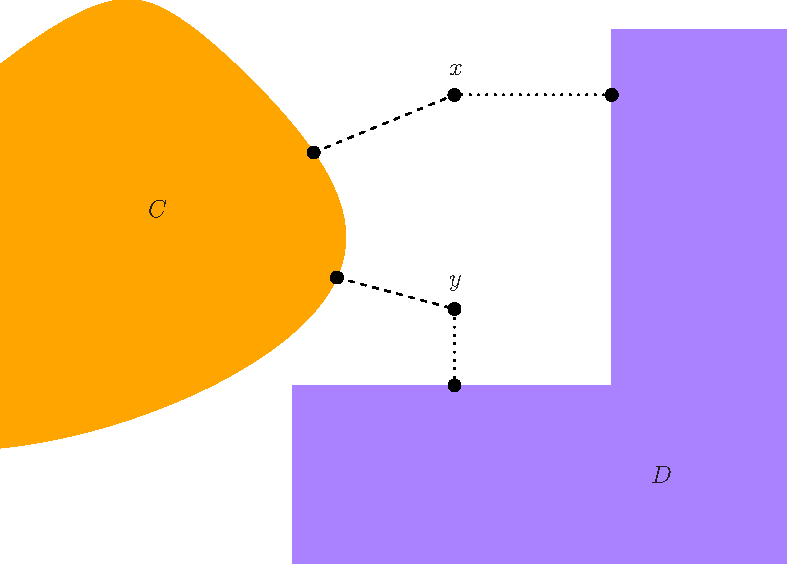
\includegraphics[width=0.65\textwidth]{fig/projection.pdf}
\caption{Illustration of properties of Euclidean projection operators onto 
  convex and nonconvex sets, $C$ and $D$. The projections of $x$ and $y$ onto
  $C$ (visualized via dashed lines) can only grow closer in Euclidean norm,
  whereas their projections onto  $D$ (dotted lines) can spread apart.}    
\label{fig:projection}
\end{figure}

\paragraph{Orthogonal decomposition.}

For a linear subspace $L$, it holds that
\index{projection!orthogonal decomposition}
\begin{equation}
\label{eq:projection_decomposition}
P_L(x) + P_{L^\perp}(x) = x, \quad \text{for all $x$},
\end{equation}
where $L^\perp = \{x : x^\T y = 0, \, \text{for all $y \in L$} \}$ denotes the
orthogonal complement of $L$, which, as it turns out, is itself a linear
subspace. An interesting application of the orthogonal decomposition property
\eqref{eq:projection_decomposition} occurs when $L = \row(A)$ and $L^\perp =
\nul(A)$, the row and null space of a matrix $A$, and this explains the
relationship between the projection maps onto $\row(A)$ and $\nul(A)$ in Example
\parref{xa:matrix_space_projection}. 

The orthogonal decomposition fact \eqref{eq:projection_decomposition} for linear
subspaces is straightforward to verify. From the variational inequality
\eqref{eq:variational_inequality} for projection onto $L$, denoting $z = P_L(x)$,
we first note that this is actually equivalent to a variational \emph{equality}
\begin{equation}
\label{eq:variational_equality}
(x - z)^\T (z - y) = 0, \quad \text{for any $y \in L$}. 
\end{equation}
as $v = z - y$ with $z, y \in L$ implies $v \in L$, and hence $-v \in L$. The 
corresponding variational equality for \smash{$z' = P_{L^\perp}(x)$} is
therefore     
\[
(x - z')^\T (z' - y') = 0, \quad \text{for any $y' \in L^\perp$}.
\]
This is satisfied for $z' = x - z$, as we get $z^\T (x - z - y') = z^\T (x -
z) + z^\T y' = 0 + 0$ for any $y' \in L^\perp$, the first term being zero due to 
\eqref{eq:variational_equality} with $y = 0$, and the second term being zero due
to the fact that $z \in L$ and $y' \in L$. This confirms \smash{$P_{L^\perp}(x) 
  = x - P_L(x)$} and proves \eqref{eq:projection_decomposition}.   

\section{Proximal nonexpansiveness*}
\label{sec:proximal_nonexpansiveness}

We examine firm nonexpansiveness of the proximal mapping. As usual, we take $f$
to be closed and convex, and $\lambda > 0$. Just as we saw for projection maps
onto convex sets, it turns out that $\prox_f$ is \emph{firmly nonexpansive},  
\index{proximal mapping!firm nonexpansiveness}
\begin{equation}
\label{eq:proximal_firm_nonexpansiveness1}
\big( \prox_{\lambda f}(x) - \prox_{\lambda f}(y) \big)^\T (x - y) \geq 
\| \prox_{\lambda f}(x) - \prox_{\lambda f}(y) \|_2^2, \quad \text{for all  
  $x,y$},   
\end{equation}
This is a powerful property, but verifying it is actually straightforward
(easier shorter than proving from first principles the corresponding result for
projections; recall Exercise \ref{ex:projection_firm_nonexpansiveness}), once we
invoke the appropriate tools: the proximal subgradient characterization, and 
subgradient monotonicity. To see this, without loss of generality, we take
$\lambda = 1$, and abbreviate $z_x = \prox_f(x)$ and $z_y = \prox_f(y)$. Observe
that 
\[
(z_x - z_y)^\T (x - y) = (z_x - z_y)^\T \big((x - z_x) - (y - z_y)\big) + 
\|z_x - z_y\|_2^2.   
\]
By the proximal subgradient characterization
\eqref{eq:proximal_subgradient_characterization}, we have $x - z_x \in \partial
f(z_x)$ and $y - z_y \in \partial f(z_y)$, and by subgradient monotonicity
\eqref{eq:subgradient_monotonicity}, the first term on the right-hand side above
is nonnegative. This proves the firm nonexpansiveness of $\prox_f$, as desired.  

Again, as in the case of projections (proved in part d of Exercise
\ref{ex:projection_firm_nonexpansiveness}), firm nonexpansiveness
\eqref{eq:proximal_firm_nonexpansiveness1} implies the more evocative  
property   
\begin{equation}
\label{eq:proximal_firm_nonexpansiveness2}
\| \prox_{\lambda f}(x) - \prox_{\lambda f}(y) \|_2^2 + 
\| (I-\prox_{\lambda f})(x) - (I-\prox_{\lambda f})(y) \|_2^2 \leq 
\|x - y\|_2^2, \quad \text{for all $x,y$}, 
\end{equation}
from which we can see that proximal \emph{nonexpansiveness} and \emph{residual
  nonexpansiveness} follow,   
\index{proximal mapping!nonexpansiveness}
\index{proximal mapping!residual nonexpansiveness} 
\begin{align}
\label{eq:proximal_nonexpansiveness}
\|\prox_{\lambda f}(x) - \prox_{\lambda f}(y)\|_2 &\leq \|x-y\|_2, 
\quad \text{for all $x,y$}, \\
\|(I-\prox_{\lambda f})(x) - (I-\prox_{\lambda f})(y)\|_2 &\leq \|x-y\|_2,
 \quad \text{for all $x,y$},
\end{align}
respectively.

\section{Moreau-Yosida regularization*}
\label{sec:moreau_envelope} 

In this last section, we return to discussing the Moreau envelope $f_\lambda$ of
a closed convex function $f$, as defined in \eqref{eq:moreau_envelope_lambda}.
Repeating its definition here for convenience, for $\lambda > 0$:
\index{Moreau envelope}
\[
f_\lambda(x) = \inf_z \bigg\{ \frac{1}{2\lambda} \|x - z\|_2^2 + f(z)
\bigg\}.
\]
The Moreau envelope $f_\lambda$ can be seen as a smoothed or regularized version
of $f$, and accordingly it is also known as \emph{Moreau-Yosida regularization}.
Figure \ref{fig:moreau_envelope} gives an illustration. We note that more can be
said about the precise connection between $f_\lambda$ and regularization, and
this will be revisited in the next chapter, from the perspective of conjugate
functions.    

\begin{figure}[tb]
\centering
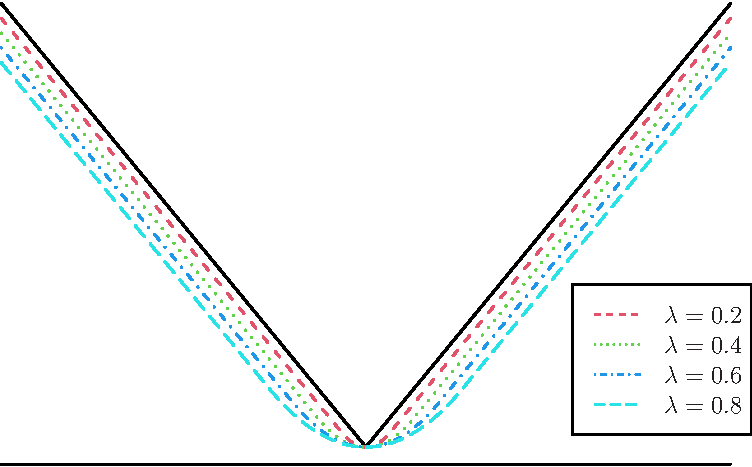
\includegraphics[width=0.625\textwidth]{fig/moreau_envelope.pdf}
\caption{Convex function (solid line) along with its Moreau envelope plotted at
  four values of $\lambda > 0$ (dashed or dotted lines of various patterns). The 
  Moreau envelope is a differentiable convex minorant to the original function,
  for any $\lambda > 0$.}    
\label{fig:moreau_envelope}
\end{figure}

Several important properties of $f_\lambda$ are apparent. First, the Moreau
envelope $f_ \lambda$ is itself convex (by Property
\parref{par:function_infimum}). Second, $f_\lambda$ has full domain,
$\dom(f_\lambda) = \R^d$, even when the original function $f$ does not. Third, 
$f$ is minorized by its Moreau envelope,
\[
f_\lambda(x) \leq f(x), \quad \text{for all $x$}.
\]
Fourth, it is not hard to see that $f_\lambda$ and $f$ have the same set of
minimizers (Exercise \ref{ex:moreau_envelope} part a):
\begin{equation}
\label{eq:moreau_envelope_argmin}
\argmin_x \, f_\lambda(x) = \argmin_x \, f(x),
\end{equation}
which means that minimization of $f$ and of $f_\lambda$ are equivalent
problems. Fifth, a property tied to the fourth one  (Exercise
\ref{ex:moreau_envelope} part b), the point $z = \prox_{\lambda f}(x)$ achieves
the infimum in \eqref{eq:moreau_envelope_lambda}, that is,   
\begin{equation}
\label{eq:moreau_envelope_prox}
f_\lambda(x) = \frac{1}{2\lambda} \|x - \prox_{\lambda f}(x)\|_2^2 + 
f \big( \prox_{\lambda f}(x) \big).
\end{equation}
Sixth, and perhaps most importantly, the Moreau envelope $f_\lambda$ is 
differentiable, and satisfies  
\index{Moreau envelope!gradient}
\begin{equation}
\label{eq:moreau_envelope_gradient}
\nabla f_\lambda(x) = \frac{1}{\lambda} \big( x - \prox_{\lambda f}(x) \big).  
\end{equation}
This fact is always true regardless of the smoothness of $f$; it is not as
immediately apparent as the above facts, and its proof is outlined in Exercise
\ref{ex:moreau_envelope} parts c and d.  

This latter property, on smoothness of the Moreau envelope, is useful for many
reasons. First, it has important algorithmic implications, because minimization
of $f$ and $f_\lambda$ are equivalent problems
\eqref{eq:moreau_envelope_argmin}, and the latter function is always smooth and
admits a clean formula for its gradient, as seen in
\eqref{eq:moreau_envelope_gradient}. Second, it has gives a more rigorous
perspective on the approximation presented in
\eqref{eq:proximal_gradient_step_approx}: rearranged, it says that for all $x$
and all $\lambda > 0$, we have the equality
\[
\prox_{\lambda f}(x) = x - \lambda \nabla f_\lambda(x).
\]
For small enough values of $\lambda$, the Moreau envelope $f_\lambda$ and the
original function $f$ will be similar, as will their gradients. This supports
the idea of substituting $\nabla f(x)$ for $\nabla f_\lambda(x)$ on the
right-hand side above, which yields \eqref{eq:proximal_gradient_step_approx}.       

The third implication of the gradient relation
\eqref{eq:moreau_envelope_gradient} requires a bit more background to
explain. It turns out that the Moreau envelope is a uniquely identifying
transform, in the following sense: if two closed convex functions have matching
Moreau envelopes, then they must be the same function. Furthermore, the
relationship between the proximal operator and the gradient of the Moreau
envelope \eqref{eq:moreau_envelope_gradient} then transfers this identifiability
property to the former (up to an additive constant). These results are stated
next, to conclude the chapter.      

\index{Moreau envelope!identification theorem}
\index{proximal mapping!identification theorem}
\begin{Theorem}
\label{thm:moreau_proximal_identification}
For closed convex $f,g : \R^d \to (-\infty, \infty]$ with nonempty domains, the
following properties hold, for any fixed $\lambda > 0$: 
\begin{enumerate}[label=(\roman*)]
\item if $f_\lambda = g_\lambda$, then $f = g$; 
\item if $\prox_{\lambda f} = \prox_{\lambda g}$, then $f = g + c$, for some
  constant $c \in \R$.  
\end{enumerate} 
\end{Theorem}

% Theorem 3.34 and Corollary 3.37 in Rockafellar and Wets (2009)

We call this the \emph{identification theorem} for Moreau envelopes and proximal
mappings; its proof is outlined in Exercise
\ref{ex:moreau_proximal_identification}.  

\SkipTocEntry\section*{Chapter notes}

The notion of a proximal mapping is due to Jean Jacques Moreau, who published
seminal work on the topic in the early and mid 1960s. Moreau studied the ways in
which proximal maps generalize projections, and developed (what is now called)
the Moreau envelope. The Moreau envelope is also sometimes called Moreau-Yosida
regularization, to pay homage to earlier related work in functional analysis by
Kosaku Yosida (cf.\ the Yosida approximation of operators). For readers seeking
to learn more about proximal operators, including extensive and important
historical references, we refer to \cite{rockafellar2009variational} (Chapters
1.G, 2.D, 3.D). We also refer to the recent monograph \cite{parikh2013proximal},
which offers numerous interesting interpretations and examples, and useful 
references. The connection between the proximal map and the resolvent of the
subdifferential operator is due to \cite{rockafellar1976monotone}. For an
elegant treatment of this and related topics from the perspective of monotone
operators, see \cite{bauschke2011convex}.

The proximal map of the total variation (TV) seminorm defines a minimization
problem known as \emph{total variation denoising}. This was proposed by
\cite{rudin1992nonlinear}, and led to a large following in research across
applied mathematics, signal processing, and statistics. An important
contribution in statistics that develops this idea further, under the name
\emph{fused lasso}, is \cite{tibshirani2005sparsity}. The taut string algorithm
for TV denoising---that is, for computing the proximal map of the TV
seminorm---was developed by \cite{davies2001local}, building on earlier work by
\cite{mammen1997locally}. A dynamic programming approach for solving the TV
denoising problem was given in \cite{johnson2013dynamic}. The taut string and
dynamic programming algorithms are both linear-time. To be clear, this is all in
reference to the univariate TV denosing problem; for generalizations defined
over multivariate lattices or arbitrary undirected graphs, the computation can
be more challenging. Important algorithmic contributions to more general TV 
denoising settings include \cite{chambolle2009total, chambolle2011first,
  barbero2018modular}, among many others. 

The sorted $\ell_1$ penalty (SLOPE) was proposed by \cite{bogdan2015slope}. 
These same authors presented a fast algorithm for its proximal map by reducing
the problem to isotonic projection, which can be solved in linear-time using the
pool adjacent violators algorithm (PAVA) of \cite{barlow1972statistical}. See
also \cite{deleeuw2010isotonic} for a nice review of various fast algorithms for
isotonic regression and related problems. Projection onto the probability
simplex (and projection onto the $\ell_1$ ball, which is reducible to the
former) can be done in in nearly linear-time with a deterministic algorithm, or
expected linear-time with a randomized algorithm, see \cite{duchi2008efficient, 
  condat2016fast}.   

Insights into the proximal decomposition phenomenon
\eqref{eq:proximal_general_sum}, including fairly general sufficient conditions,
were given in \cite{yu2013decomposing}. This reproduces (and generalizes)
previously known results about proximal decomposition in special cases, such as 
those found in \cite{friedman2007pathwise} on the elastic net and fused lasso
penalties. Exercise \ref{ex:proximal_general_sum} below is based on
\cite{yu2013decomposing}.    

\clearpage

\begin{xcb}{Exercises}
\begin{enumerate}[label=\thechapter.\arabic*]
\settowidth{\leftmargini}{0.00.\hskip\labelsep}

\item \label{ex:lp_norm_proximal_mapping} 
  We establish the proximal results for the $\ell_1$, $\ell_2$, and $\ell_0$
  norms in Example \ref{xa:proximal_mappings}. 

\begin{enumerate}[label=\alph*.]
\index{l1 norm@$\ell_1$ norm!proximal mapping}
\index{soft-thresholding}
\item Using the subgradient characterization
  \eqref{eq:proximal_subgradient_characterization} and the subgradients
  of the $\ell_1$ norm from Example \parref{xa:l1_norm_subgradients}, prove the
  result in Example \parref{xa:l1_norm_proximal_mapping}.

\item Using the subgradient characterization
  \eqref{eq:proximal_subgradient_characterization} and the subgradients
  of the $\ell_2$ norm from Example \parref{xa:lp_norm_subgradients}, prove the
  result in Example \parref{xa:l2_norm_proximal_mapping}.

\index{l0 norm@$\ell_0$ norm!proximal mapping}
\index{hard-thresholding}
\item Now prove the result in Example \parref{xa:l0_norm_proximal_mapping} on 
  the $\ell_0$ norm, by breaking the argument down into cases (for $|x_i| >
  \lambda$ and $|x_i| \leq \lambda$), and simply arguing directly that the
  minimizer is as claimed in each case.   
\end{enumerate}

\item \label{ex:matrix_norm_proximal_mapping1}
  We establish the proximal results for the trace and Frobenius norms in Example
  \ref{xa:proximal_mappings}. To be entirely clear, for a function $f$ defined
  on $\R^{k \times d}$, its proximal map is  
  \begin{equation}
  \label{eq:proximal_mapping_matrix}
  \prox_{\lambda f}(X) = \argmin_z \bigg\{ \frac{1}{2} \|X -
  Z\|_F^2 + \lambda f(Z) \bigg\}, 
  \end{equation}
  which is consistent with interpreting the space $k \times d$ of matrices as a
  $kd$-dimensional vector space defined by its entries, and applying the usual
  definition \eqref{eq:proximal_mapping_lambda} of the proximal map. The
  subgradient optimality condition for \eqref{eq:proximal_mapping_matrix} says  
  that $Z = \prox_{\lambda f}(X)$ if and only if
  \begin{equation}
  \label{eq:proximal_subgradient_characterization_matrix}
  X - Z \in \lambda \partial f(Z),
  \end{equation}
  which is just the appropriate translation of the subgradient characterization
  \eqref{eq:proximal_subgradient_characterization} to the matrix domain. 

\begin{enumerate}[label=\alph*.]
\index{trace norm!proximal mapping}
\index{matrix soft-thresholding}
\item Using the subgradient characterization 
  \eqref{eq:proximal_subgradient_characterization_matrix} along with the
  subgradients of the trace norm from Example
  \parref{xa:trace_norm_subgradients}, prove the result in Example
  \parref{xa:trace_norm_proximal_mapping}. 

\index{Frobenius norm!proximal mapping}
\item Using the subgradient characterization 
  \eqref{eq:proximal_subgradient_characterization_matrix}, where the
  subgradients of the Frobenius norm can derived analogously to those for the
  $\ell_2$ norm as in Example \parref{xa:lp_norm_subgradients}, prove the result
  in Example \parref{xa:frobenius_norm_proximal_mapping}.  
\end{enumerate}

\item \label{ex:matrix_norm_proximal_mapping2}
  Now we derive proximal mappings for a class of functions on $\R^{k \times d}$,
  of the form 
  \begin{equation}
  \label{eq:singular_function}
  f(X) = g(\sigma(X)), 
  \end{equation}
  for a function $g : \R^d \to \R$, where we write $\sigma(X) = (\sigma_1(X), \ldots,
  \sigma_k(X)) \in \R^k$ for the vector of singular values of $X$. An important
  example here is the \emph{Schatten $p$-norm}, defined for $p \geq 1$ as
  \index{Schatten norm}
  \begin{equation}
  \label{eq:schatten_norm}
  \|X\|_p = \|\sigma(X)\|_p,
  \end{equation}
  with $\|\cdot\|_p$ on the right-hand side denoting the usual $\ell_p$ norm on
  vectors. Note that in terms of Shatten norms (that is, the left-hand side in
  all equalities below represents a Schatten norm): 
  \begin{itemize}
  \item $\|\cdot\|_1 = \|\cdot\|_{\tr}$, the trace norm;
  \item $\|\cdot\|_2 = \|\cdot\|_F$, the Frobenius norm; and
  \item $\|\cdot\|_\infty = \|\cdot\|_{\op}$, the operator norm.  
  \end{itemize}
  An important fact about functions $f$ of the form
  \eqref{eq:singular_function}: they are \emph{unitarily invariant}, meaning 
  $f(UXV) = f(X)$ for any orthogonal matrices $U,V$ (because left- or
  right-muliplication by orthogonal matrices does not change the singular
  values).    
  
\begin{enumerate}[label=\alph*.]
\item For $X = U \Sigma V^\T$ denoting the SVD of $X$, and $\sigma = \sigma(X)$
  is the diagonal of $\Sigma$, prove   
  \[
  \prox_{\lambda f}(X) = U \diag(\prox_g(\sigma)) V^\T,
  \]
  where we use $A = \diag(a)$ to construct a diagonal matrix from a vector $a$.    

\item Using the Schatten $p$-norm connections listed above, check that the
  result from part a reproduces the results for the trace and Frobenius norms, in
  Examples \parref{xa:trace_norm_proximal_mapping} and 
  \parref{xa:frobenius_norm_proximal_mapping}.  
\index{Schatten norm!proximal mapping}
  
\item Now use the result from part a to derive the proximal map of the matrix
  rank function, from Example \parref{xa:rank_proximal_mapping}. 
\end{enumerate}

\item For \smash{$f(x) = \inf_{z \in C} \|x - z\|_2 = \|x - P_C(x)\|_2$},
  where $C$ is a closed convex set, prove that   
  \[
  \prox_{\lambda f}(x) = 
  \begin{cases}
  \displaystyle
  x - \lambda \frac{x - P_C(x)}{\|x - P_C(x)\|_2} & 
  \text{if $\|x - P_C(x)\|_2 > \lambda$} \\ 
  P_C(x) & \text{if $\|x - P_C(x)\|_2 \leq \lambda$}.
  \end{cases}
  \]
  Hint: recall that $f$ is differentiable at each $x \notin C$, with gradient
  given in \eqref{eq:set_distance_subgradients}.    

\item Prove the proximal quadratic sum rule in Property
  \parref{par:proximal_quadratic_sum}.  

\item \label{ex:generalized_enet_proximal_mapping}
  Prove the proximal decomposition fact 
  \eqref{eq:generalized_enet_proximal_mapping} for positively homogeneous 
  $f$. Hint: show that positive homogeneity implies that $\prox_{tf}(tx) = t
  \prox_f(x)$, for any $t > 0$ and any $x$; use this together with the quadratic
  sum rule from Property \parref{par:proximal_quadratic_sum} to prove the
  desired result.  

\item \label{ex:proximal_general_sum}
  In this exercise, we will establish a sufficient condition for the
  proximal decomposition given in \eqref{eq:proximal_general_sum}, following the
  development of Theorem 1 and Proposition 2 in \cite{yu2013decomposing}. Let  
  $f,g$ be closed and convex.   

\begin{enumerate}[label=\alph*.]
\item First show that, for any $x$, the point $\prox_f(\prox_g(x))$ satisfies  
  \[
  0 \in \prox_f(\prox_g(x)) - x + \partial g(\prox_g(x)) + 
  \partial f \big( \prox_f(\prox_g(x)) \big).
  \]
  Hint: use the proximal subgradient characterization
  \eqref{eq:proximal_subgradient_characterization} for $\prox_f(\prox_g(x))$, 
  as well as for $\prox_g(x)$, and add these two expressions together. 

\item Assume that 
  \begin{equation}
  \label{eq:proximal_decomposition_condition1}
  \partial g(x) \subseteq \partial g(\prox_f(x)), \quad \text{for all $x$}. 
  \end{equation}
  Show that, for any $x$, the point $\prox_f(\prox_g(x))$ must then satisfy   
  \[
  0 \in \prox_f(\prox_g(x)) - x + \partial g \big( \prox_f(\prox_g(x)) \big) +  
  \partial f \big( \prox_f(\prox_g(x)) \big).
  \]
  Hint: use part a. Conclude using the subgradient characterization for
  $\prox_{f+g}(x)$ and single-valuedness of the proximal map that
  $\prox_{f+g}(x) = \prox_f(\prox_g(x))$, and as $x$ was arbitrary,
  $\prox_{f+g} =  \prox_f \circ \prox_g$.   

\item Let \smash{$g = \sum_{i=1}^k g_i$}, with each $g_i$ closed and convex, 
  and \smash{$\cap_{i=1}^k \relint(\dom(g_i)) \not= \emptyset$}. Prove that
  \eqref{eq:proximal_decomposition_condition1} is implied by
  \begin{equation}
  \label{eq:proximal_decomposition_condition2}
  \partial g_i(x) \subseteq \partial g_i(\prox_f(x)), \quad \text{for all $x$, 
    and $i=1,\ldots,k$},  
  \end{equation}
  and thus the latter is a sufficient condition for $\prox_{f+g} =  \prox_f \circ
  \prox_g$. 
\end{enumerate}

\item \label{ex:generalized_tv_proximal_mapping}
  Now we follow the development of Corollary 4 in \cite{yu2013decomposing}. Let
  $g$ be a polyhedral function, 
  \[
  g(x) = \max_{i=1,\ldots,k} \, a_i^\T x.
  \]
  
\begin{enumerate}[label=\alph*.]
\item Show that the sufficient condition in
  \eqref{eq:proximal_decomposition_condition2}, from Exercise
  \ref{ex:proximal_general_sum} part c, is equivalent to  
  \[
  \prox_g(K_i) \subseteq K_i, \quad i=1,\ldots,k,
  \]
  where each $K_i = \{x : a_i^\T x = g(x)\}$ is a polyhedral cone. Hint: use the
  subgradient rule for a pointwise maximum from Property
  \parref{par:subgradient_supremum}.   

\item Let $f$ be permutation invariant, which means that $f(x) = f(x_\pi)$, for
  all $x$ and permutations $\pi$ (where we denote \smash{$x_\pi = (x_{\pi_1},
    \ldots, x_{\pi_d})$} for $\pi=(\pi_1,\ldots,\pi_d)$). Show that $\prox_f$ is
  then order-preserving,  
 \[
 x_i \geq x_j \implies [\prox_f(x)]_i \geq [\prox_f(x)]_j, \quad \text{for all
   $x \in \R^d$ and $i,j$}.
 \]

\item Let \smash{$\|x\|_{\TV} = \sum_{(i,j) \in E} |x_i - x_j|$} be a
  generalized TV seminorm, defined with respect to an edge set $E$ (notice that  
  this generalizes \eqref{eq:tv}, which corresponds to $E = \{(i, i+1) : i =
  1,\ldots,d-1\}$. Prove that \eqref{eq:generalized_tv_proximal_mapping} holds
  for any permutation invariant $f$ and any edge set $E$. Hint: check that the
  condition in part a holds, for the appropriate instantiation of cones $K_i$,
  $i=1,\ldots,k$; and for this, use the order-preserving property from part b.   
\index{total variation (TV) penalty!proximal mapping}
\end{enumerate}

\item \label{ex:proximal_linear}
  We examine linear composition rules for proximal mappings. 

\begin{enumerate}[label=\alph*.]
\item Prove the rule in Property \parref{par:proximal_linear} for orthogonal $A$
  (that is, $A^\T A = A A^\T = I$).   

\item Prove that more generally, if $A$ has orthonormal rows (and it need not be 
  square), and $b \in \R^d$ is arbitrary, then $F(x) = f(Ax + b)$ has proximal
  mapping 
  \[
  \prox_F(x)  = x - A^\T \big(Ax + b - \prox_f(Ax + b) \big).
  \]
\end{enumerate}
  
\index{proximal mapping!fixed-point equation}
\item \label{ex:proximal_optimality_fg}
  In this exercise, we prove that the fixed-point equation 
  \eqref{eq:proximal_optimality_fg} is necessary and sufficient for minimizing
  $F = f+g$, where $f,g$ are closed and convex and $f$ is differentiable. Let
  $\lambda > 0$ be arbitrary.

\begin{enumerate}[label=\alph*.]
\item Show that $x$ minimizes $F$ if and only if
  \[
  x - \lambda \nabla f(x) \in x + \lambda \partial g(x).
  \]
  % TODO: do we need \relint(\dom(f)) \cap \relint(\dom(g)) \not= \emptyset? 
  
\item Show that the above display is equivalent to
  \eqref{eq:proximal_optimality_fg} using the resolvent characterization     
  $\prox_{\lambda g} = (I + \lambda \partial g)^{-1}$, and the fact that this
  inverse is single-valued. 
\end{enumerate}

\index{projection!onto $\ell_1$ ball}
\index{probability simplex!projection}
\item \label{ex:l1_projection}
  Consider the projection problems for the probability simplex and the unit
  $\ell_1$ ball, 
  \begin{align}
  \label{eq:simplex_projection}
  &\minimize_z \quad \|x - z\|_2^2 \quad \st \quad \one^\T x = 1, 
    \; x \geq 0, \\ 
  \label{eq:l1_projection}
  &\minimize_z \quad \|x - z\|_2^2 \quad \st \quad \|x\|_1 \leq 1,
  \end{align}
  respectively. 

\begin{enumerate}[label=\alph*.]
\item Starting with \eqref{eq:l1_projection}, show that if $z$ is a solution,
  then $\sign(z_i) = \sign(x_i)$, $i=1,\ldots,d$. 

\item Use part a to argue that we can reduce any $\ell_1$ projection to a
  simplex projection; that is, in order to solve \eqref{eq:l1_projection}, we
  can first solve a problem of the form \eqref{eq:simplex_projection} and then
  we can postprocess the solution to obtain a solution to the original problem.     
\end{enumerate}  

\index{projection!firm nonexpansiveness}
\item \label{ex:projection_firm_nonexpansiveness}
  This exercise investigates firm nonexpansiveness
  \eqref{eq:projection_firm_nonexpansiveness1} of the projection operator $P_C$
  onto a convex set $C$. For any $x,y$, let us abbreviate $p_x = P_C(x)$ and
  $p_y = P_C(y)$. From the variational inequality
  \eqref{eq:variational_inequality}, note that     
  \begin{align*}
  (x - p_x)^\T (p_x - y) \geq 0, \\
  (y - p_y)^\T (p_y - x) \geq 0.
  \end{align*}

\begin{enumerate}[label=\alph*.]
\item Use the above pair of inequalities to prove that 
  \[
  \big( x - p_x - (y - p_y) \big)^\T (p_x - p_y) \geq 0, \quad \text{for all
    $x,y$}. 
  \]
  Hint: expand $p_x - y = p_x - p_y + p_y - y$ in the first inequality, $p_y - x
  = p_y - p_x + p_x - x$ in the second inequality, then subtract the two and
  simplify.   
  
\item Show that the condition from part a is equivalent to firm nonexpansiveness 
  \eqref{eq:projection_firm_nonexpansiveness1}, and show that it also equivalent
  to   
  \[
  (r_x - r_y)^\T (x - y) \geq \|r_x - r_y\|_2^2, \quad \text{for all $x,y$},
  \]
  where we abbreviate $r_x = x - P_C(x)$ and $r_y = x - P_C(y)$.

\item Show using the Cauchy-Schwarz inequality that
  \eqref{eq:projection_firm_nonexpansiveness1} implies
  \eqref{eq:projection_nonexpansiveness}. Show similarly using part b and the
  Cauchy-Schwarz inequality that \eqref{eq:projection_firm_nonexpansiveness1}
  implies \eqref{eq:projection_residual_nonexpansiveness}.

\item Show finally that firm nonexpansiveness implies 
  \[
  \|p_x - p_y\|_2^2 + \|r_x - r_y\|_2^2 \leq \|x - y\|_2^2, \quad \text{for all
    $x,y$},
  \]
  which gives another way of seeing that
  \eqref{eq:projection_firm_nonexpansiveness1} leads to both
  \eqref{eq:projection_nonexpansiveness} and
  \eqref{eq:projection_residual_nonexpansiveness}. 
\end{enumerate}

\index{proximal mapping!contractiveness}
\index{proximal mapping!fixed-point equation}
\item In this exercise, we study a \emph{contractive} property of proximal
  operators (and projections): for closed convex $f$ and $\lambda > 0$, show
  that if $f(x^\star) = f^\star = \inf_x f(x)$, then   
  \[
  \| \prox_{\lambda f}(x) - x^\star\|_2 < \|x - x^\star\|_2, \quad \text{for
    all $x$ with $f(x) > f^\star$}.
  \]
  Note the strict inequality. In the special case of $f = I_C$, the
  characteristic function of a closed convex set $C$, this reduces to 
  \[
  \| P_C(x) - y\|_2 < \|x - y\|_2, \quad \text{for all $x \notin C$ and $y \in
    C$}.    
  \]
  Hint: recall the implication \eqref{eq:proximal_firm_nonexpansiveness2} from
  firm nonexpansiveness, and the proximal fixed-point characterization of 
  minimizers in \eqref{eq:proximal_optimality}.  

\item \label{ex:moreau_envelope}
  We examine key facts about the Moreau envelope $f_\lambda$ of a closed convex
  function $f$, for $\lambda > 0$. 

\begin{enumerate}[label=\alph*.]
\item Prove that $f$ and $f_\lambda$ have the same minimizers, as in
  \eqref{eq:moreau_envelope_argmin}. Hint: apply the subgradient optimality
  condition to the definition of $f_\lambda$.   

\item Show that the subgradient calculation from part a implies
  \eqref{eq:moreau_envelope_prox}. 

\item Prove that if we already knew that $f_\lambda$ was differentiable, then
  its gradient must be as in \eqref{eq:moreau_envelope_gradient}, by using the
  subgradient rule for a partial infimum in Property
  \parref{par:subgradient_infimum}.   

\index{Moreau envelope!gradient}
\item Now prove that $f_\lambda$ is differentiable with gradient as given in
  \eqref{eq:moreau_envelope_gradient}. Hint: abbreviating $f_x = f_\lambda(x)$
  and $z_x = \prox_{\lambda f}(x)$, simply verify the definition of
  differentiability directly: 
  \[
  \lim_{y \to x} \frac{f_y - f_x - (y - x)^\T (x - z_x) / \lambda}{\|y-x\|_2^2} 
  = 0.
  \]
  To check this, use \eqref{eq:moreau_envelope_prox} and direct algebra to argue 
  that $f_y - f_x \geq (y - x)^\T (x - z_x) / \lambda$; by swapping the roles of
  $x$ and $y$, argue that also $f_y - f_x \leq (y - x)^\T (y - z_y) / \lambda$. 
  These two inequalities can be used in combination to verify the
  differentiability condition.     
\end{enumerate}

\item Let $f(x) = |x|$. Prove that its Moreau envelope $f_\lambda$ is the 
  \emph{Huber function} (which is commonly used as a loss in robust statistics,
  being smooth and having linear growth away from zero): 
  \index{Huber function}
  \[
  f_\lambda(x) = 
  \begin{cases}
  x^2/ (2\lambda) & \text{if $|x| \leq \lambda$} \\
  |x| - \lambda/2 & \text{if $|x| > \lambda$}.
  \end{cases}
  \]
  This is in fact the Moreau envelope that is visualized in Figure
  \ref{fig:moreau_envelope}.  

\index{Moreau envelope!identification theorem}
\index{proximal mapping!identification theorem}
\item \label{ex:moreau_proximal_identification}
  In this exercise, we prove the identification theorem, Theorem
  \ref{thm:moreau_proximal_identification}, for Moreau envelopes and proximal
  maps. Following the development of Theorem 3.34 in
  \cite{rockafellar2009variational}, it helps to introduce the general concept 
  of an \emph{infimal convolution} of functions $f,g$: 
  \index{infimal convolution}
  \[
  (f \infconv g)(x) = \inf_z \Big\{ f(z) + g(x-z) \Big\}.
  \]
  In this notation, observe that \smash{$f_\lambda = f \infconv \|\cdot\|_2^2 / 
    (2\lambda)$}, that is, the Moreau envelope is the infimal convolution of $f$
  and the map $x \mapsto \|x\|_2^2 /  (2\lambda)$. Below, let $f,g$ be closed
  and convex.   

\begin{enumerate}[label=\alph*.]
\item Assume that $f \infconv h = g \infconv h$ for a closed, convex, and
  coercive function $h$. Prove that for any value of $\lambda > 0$,  
  \[
  \inf_x \Big\{ f_\lambda(x) - v^\T x \Big\} = \inf_x \Big\{ g_\lambda(x) - v^\T
  x \Big\}, \quad \text{for all $v$}.
  \]
  Hint: first observe that $f_\lambda \infconv h = g_\lambda \infconv h$ by the
  commutative property of infimal convolutions. Then use basic algebra to
  decompose \smash{$\inf_x \, \{ f_\lambda \infconv h(x) - v^\T x \}$} into two 
  terms, one depending only on $f_\lambda$, and the other only on $h$. Compare
  this to the expression we get when $f$ is replaced by $g$. 

\item Now under the same assumption $f \infconv h = g \infconv h$, show that $f
  = g$. Hint: if $f \not= g$ then for some $x$ we will have (without a loss of
  generality) $f(x) > g(x)$, and thus $f_\lambda(x) > g_\lambda(x)$ for small 
  enough $\lambda > 0$. Show that for $v = \nabla f_\lambda(x)$, we get   
  \[
  \inf_y \Big\{ f_\lambda(y) - v^\T y \Big\} = 
  f_\lambda(x) - v^\T x > g_\lambda(x) - v^\T x \geq 
  \inf_y \Big\{ g_\lambda(y) - v^\T y \Big\},
  \]
  which would violate the result from part a.

\item Fix $\lambda > 0$. Apply the result from part b to $h(x) =
  \|x\|_2^2/(2\lambda)$, in order to prove part (i) in Theorem
  \ref{thm:moreau_proximal_identification}. Use the gradient relation
  \eqref{eq:moreau_envelope_gradient} to prove part (ii) in the theorem.  
\end{enumerate}

\index{scaled proximal mapping}
\item \label{ex:scaled_proximal_mapping}
  We explore a generalization of the proximal map known as the \emph{scaled 
    proximal map}. We fix a positive definite matrix $H \succ 0$, and then
  define the scaled proximal mapping with respect to $H$, acting on a given
  function $f$, by   
  \begin{equation}
  \label{eq:scaled_proximal_mapping}
  \prox_f^H(x) = \argmin_z \bigg\{ \frac{1}{2} \|x - z\|_H^2 + f(z) \bigg\}, 
  \end{equation}
  where $\|\cdot\|_H$ denotes the scaled Euclidean norm, defined by $\|x\|_H^2 = 
  x^\T H x$. The parts of this exercise that follow walk through several nice
  properties of the scaled proximal mapping \eqref{eq:scaled_proximal_mapping},
  generalizing those of the (unscaled) proximal mapping
  \eqref{eq:proximal_mapping_lambda}. Note that the former is a special case of 
  the latter with $H = (1/\lambda) I$, with $I$ denoting the identity
  matrix. Below $f$ is assumed to be closed and convex.  

\begin{enumerate}[label=\alph*.]
\item \emph{Existence and uniqueness.} Prove that the minimizer in
  \eqref{eq:scaled_proximal_mapping} exists and is unique.

\item \emph{Subgradient characterization.} Prove that \smash{$z = \prox_f^H(x)$}
  if and only if $H(x - z) \in \partial f(z)$. 

\item \emph{Steepest descent interpretation.} Argue (using heuristic arguments)
  that 
  \[
  \prox_f^H(x) \approx x - H^{-1} \nabla f(x),
  \] 
  which we can interpret as performing a steepest descent step starting at $x$,
  which respect to the scaled norm $\|\cdot\|_H$. 

\item \emph{Resolvent characterization.} Prove that \smash{$\prox_f^H = (H +
    \partial f)^{-1} H$}, where the inverse here is interpreted as
  single-valued.   

\item \emph{Fixed-point equation.} Prove that $x$ minimizes $f$ if and only if
  \smash{$x = \prox_f^H(x)$}; furthermore, $x$ minimizes $F = f+g$ for closed
  convex $f,g$, with $f$ differentiable, if and only if    
  \[
  x = \prox_g^H \big( x - H^{-1} \nabla f(x) \big).
  \]

\item \emph{Firm nonexpansiveness.} Prove that \smash{$\prox_f^H$} is firmly
  nonexpansive in the $\|\cdot\|_H$ norm, 
  \[
  \big( \prox_f^H(x) - \prox_f^H(y) \big)^\T (x - y) \geq 
  \| \prox_f^H(x) - \prox_f^H(y) \|_H^2, \quad \text{for all $x,y$}.   
  \]
  Show that this in turn implies that it is both nonexpansive and residual
  nonexpansive, again in the $\|\cdot\|_H$ norm.
\end{enumerate}
\end{enumerate}
\end{xcb}
\chapter{Convex conjugates}
\label{chap:convex_conjugates}

This chapter introduces a concept that is deeply connected to subgradients and
proximal mappings (as covered in the last two chapters), and to duality theory
(as will be covered next). In fact, just as with subgradients, proximal maps,
and duality, the topic of the current chapter is at the same time quite simple
and quite powerful.      

\section{Definition and properties}

Given a function $f : \R^d \to [-\infty, \infty]$, its \emph{convex conjugate}
$f^*$ (also simply called its conjugate) is another function on $\R^d$ defined
as        
\index{conjugate}
\begin{equation}
\label{eq:conjugate}
f^*(u) = \sup_x \, \Big\{ u^\T x - f(x) \Big\}.
\end{equation}
The mapping from $f \mapsto f^*$ is also called the \emph{Legendre-Fenchel
  transform}. At the outset, we remark that $f^*$ is always convex, by the
partial supremum rule in Property \parref{par:function_supremum} (the map
$u \mapsto u^\T x - f(x)$ is affine and thus convex for each $x$). 
Moreover, the function $f^*$ is always closed, since its epigraph can be
expressed as an intersection of closed halfspaces, which is a closed set
(Exercise \ref{ex:conjugate_closed}). To be clear, these properties---the
closedness and convexity of $f^*$---hold regardless of whether $f$ itself is
closed or convex.      

A useful interpretation of $f^*$ is as follows: at each point $u$, the value
$f^*(u)$ is the maximum gap between a linear function with ``slope'' $u$ and
$f$. Figure \ref{fig:conjugate} gives an illustration. This interpretation
suggests that there may be some interesting geometry at play that underlies the
convex conjugate, which we revisit shortly when we discuss double conjugation.      

\begin{figure}[tb]
\centering
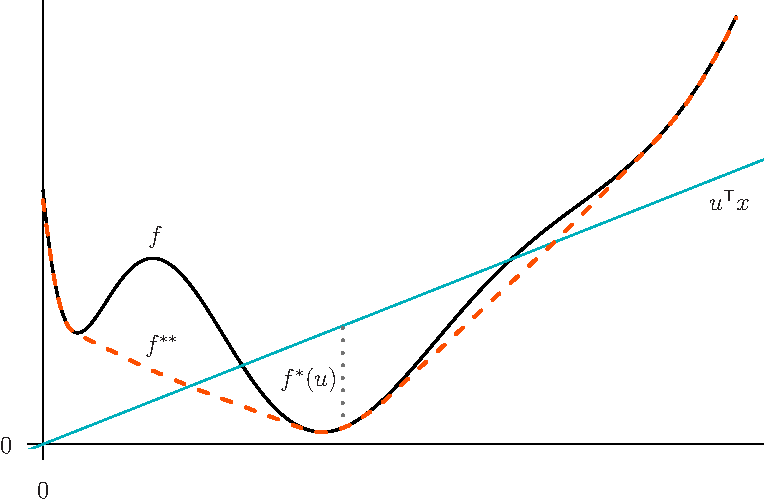
\includegraphics[width=0.7\textwidth]{fig/conjugate.pdf}
\caption{The conjugate $f^*$ evaluated at $u$ is the maximum gap between a
  linear function with slope $u$ and $f$, illustrated by the dotted line. The
  double conjugate $f^{**}$ is the pointwise supremum of all affine minorants to
  $f$ (equivalently, the greatest closed convex minorant to $f$), illustrated by
  the dashed line.}     
\label{fig:conjugate}
\end{figure}

Next we describe several important properties of convex conjugates. We generally
assume that $f \not= \infty$ ($\dom(f) \not= \emptyset$) henceforth to avoid 
trivialities when studying convex conjugates.        

\paragraph{Fenchel's inequality.}

For any $u$, observe that by the definition of the convex conjugate
\eqref{eq:conjugate} it holds that $f^*(u) \geq u^\T x - f(x)$, for any
$x$. Rearranging yields what is called \emph{Fenchel's inequality}, 
\index{Fenchel's inequality}
\begin{equation}
\label{eq:fenchel_inequality}
f(x) + f^*(u) \geq x^\T u, \quad \text{for all $x,u$}.
\end{equation}
Equality holds in \eqref{eq:fenchel_inequality} if and only if $x$ achieves the
supremum in \eqref{eq:conjugate}. As we show next, this can be further
characterized using subgradients of $f$.   

\paragraph{Subgradient equivalences.}

The supremum in \eqref{eq:conjugate} is attained at $x$ if and only if $x$
solves  
\[
\minimize_x \quad f(x) - u^\T x,
\]
which for convex $f$ is equivalent to $0 \in \partial f(x) - u$, that is, $u \in 
\partial f(x)$, using subgradient optimality. (Note that we use convexity 
of $f$ to split the subdifferential of a sum into a sum of subdifferentials, by 
Property \parref{par:subgradient_sum}.)  Meanwhile, by the rule for subgradients
of a partial supremum (Property \parref{par:subgradient_supremum}) we know that
$\partial f^*(u)$ contains all points of the form 
\[
\nabla_u \big( u^\T x - f(x) \big) = x,
\]
such that $x$ that achieves the supremum in \eqref{eq:conjugate}. In fact, if
$f$ is \emph{closed} and convex, then using the fact that $f^{**} = f$, to be 
established below, we can conclude that this describes \emph{all} of the
elements of $\partial f^*(u)$ (Exercise \ref{ex:conjugate_subgradients}). The 
next result records these equivalences. 

\index{conjugate!subgradients}
\begin{Theorem}
\label{thm:conjugate_subgradients}
For closed and convex $f$ with nonempty domain, the following statements are all 
equivalent:
\begin{enumerate}[label=(\roman*)]
\item $x$ achieves the supremum in \eqref{eq:conjugate};
\item $f(x) + f^*(u) = x^\T u$;
\item $u \in \partial f(x)$;
\item $x \in \partial f^*(u)$.
\end{enumerate}
\end{Theorem}
\vspace{-3pt}

\paragraph{Double conjugation.}

The conjugate of $f^*$ is known as the \emph{double conjugate} of $f$ and
denoted $f^{**}$. Simply applying the definition \eqref{eq:conjugate} with $f^*$
in place of $f$, we get 
\index{conjugate!double}
\begin{equation}
\label{eq:double_conjugate}
f^{**}(x) = \sup_u \, \Big\{ x^\T u - f^*(u) \Big\},
\end{equation}
and by the same rationale given previously, we note that $f^{**}$ is always
closed and convex. Applying Fenchel's inequality \eqref{eq:fenchel_inequality},
that is, $f^*(u) \geq x^\T u - f(x)$, to the term inside the supremum gives    
\[
f^{**} \leq f,
\]
or, in other words, the double conjugate $f^{**}$ minorizes the original
function $f$. In fact, the double conjugate function $f^{**}$ is not just any
(convex) minorant of $f$, it is the pointwise supremum of all affine minorants
of $f$ (Exercise \ref{ex:double_conjugate_affine_minorant}):       
\begin{equation}
\label{eq:double_conjugate_affine_minorant} 
f^{**}(x) = \sup \{ g(x) : \text{$g$ is affine, and $g \leq f$} \}, \quad
\text{for all $x \in \dom(f)$}. 
\end{equation}
See Figure \ref{fig:conjugate} again for an illustration. Lastly, an important
special reduction occurs for closed and convex $f$: in this case, we get   
\begin{equation}
\label{eq:double_conjugate_reduction}
f^{**} = f.
\end{equation}
Exercises
\ref{ex:affine_minorant_revisited}--\ref{ex:double_conjugate_reduction} walk
through the proof of this and related facts.

\medskip

\begin{Example}
Below are examples of convex conjugates for some functions of interest. The
calculations for most are straightforward; for others we defer the details to
exercises.   

\begin{enumerate}[label=\alph*., ref=\alph*]
\item \parlab{xa:quadratic_conjugate}
  For $f(x) = \frac{1}{2} x^\T Q x$, where $Q \succ 0$, its conjugate is $f^*(u)
  = \frac{1}{2} u^\T Q^{-1} u$.  

\item For $f(x) = \sum_{i=1}^d \log(1+e^{x_i})$, its conjugate is 
  \[
  f^*(u) = \sum_{i=1}^d \big( u_i \log(u_i) + (1-u_i) \log(1-u_i) \big), 
  \] 
  with $\dom(f^*) = [0,1]^d$ (and where we interpret $0 \log(0) = 0$). 

\item For $f(x) = \sum_{i=1}^d x_i \log(x_i)$, its conjugate is $f^*(u) =
  \sum_{i=1}^d \exp(u_i - 1)$. 
\index{negative entropy function!conjugate}

\item \parlab{xa:characteristic_function_conjugate}   
  For $f = I_C$, the characteristic function of an arbitrary set $C$, its
  conjugate is \vphantom{$\sum_{i=1}^d$} 
  \index{characteristic function!conjugate}
  \[
  f^* = h_C,
  \]
  where recall \smash{$h_C(u) = \sup_{x \in C} \, u^\T x$} denotes the support
  function corresponding to $C$.  

\item \parlab{xa:support_function_conjugate} 
  For $f = h_C$, the support function corresponding to a closed, convex, and
  nonempty set $C$, its conjugate is (Exercise
  \ref{ex:support_function_conjugate}):    
  \index{support function!conjugate} 
  \[
  f^* = I_C,
  \]
  the characteristic function of $C$. 

\item \parlab{xa:norm_conjugate}  
  For $f(x) = \|x\|$, where $\|\cdot\|$ is an arbitrary norm, its conjugate is
  (Exercise \ref{ex:norm_conjugate}):  
  \index{norm!conjugate}
  \index{dual norm}
  \[
  f^* = I_{\{u \,:\, \|u\|_* \leq 1\}},
  \]
  the characteristic function of the unit ball in the dual norm
  $\|\cdot\|_*$.
\end{enumerate}
\end{Example}

\section{Conjugate calculus}

We describe rules that will be helpful in calculating convex conjugates.  

\paragraph{Scaling.}
\parlab{par:conjugate_scaling}

It helps to first introduce some notation. For a function $f$ and $a>0$, we
write $af$ to denote the function defined by $(af)(x) = af(x)$, whereas we write
$fa$ for the function defined by $(fa)(x) = af(x/a)$. We refer to the operation
$f \mapsto af$ as \emph{left scaling}, and the operation $f \mapsto fa$ as
\emph{right scaling}.

Now we are ready to describe the relationship between scaling and conjugacy: for
any function $f$ and $a>0$, it holds that $(fa)^* = af^*$. Moreover, for closed 
and convex $f$, we have $(af)^* = f^*a$. In short, for closed and convex
functions, left and right scaling are dual operations under conjugacy. 

\paragraph{Translation.}

The simplest translation rule is as follows: for any function $f$ and $a \in
\R$, writing $f+a$ for the function defined by $(f+a)(x) = f(x)+a$, it holds
that $(f+a)^* = f^*-a$. That is, addition and subtraction by a real constant are
dual to each other.

Another translation rule: if $F(x) = f(x-a)$, for any $f$ and $a \in \R^d$, then
$F^*(u) = f^*(u) + a^\T u$, and if $F(x) = f(x) + a^\T x$, then $F^*(u) =
f^*(u-a)$. That is, translation of the domain by a vector $a$ and addition by a
linear function with ``slope'' $a$ are dual to each other. 

\paragraph{Linear composition.}

Similar to scaling, we first introduce some notation. For $A \in \R^{d \times
  k}$, and a function $f$ on $\R^d$, we write $fA$ to denote the function (on
$\R^k$) defined by $(fA)(x) = f(Ax)$. Also, for a function $f$ on $\R^k$, we
write $Af$ to denote the function (on $\R^d$) defined by 
\[
(Af)(y) = \inf_{Ax=y} \, f(x).
\]
We refer to the operation $f \mapsto Af$ as \emph{left composition}, and $f
\mapsto fA$ as \emph{right composition}.

Now we can describe the relationship between composition and conjugacy: for any
function $f$ on $\R^k$ and $A \in \R^{d \times k}$, it holds that $(Af)^* =
f^*A^\T$. Moreover, for a closed and convex function $f$ on $\R^d$, we have 
$(fA)^* = A^\T f^*$. In other words, for closed and convex functions, left and
right composition are dual to each other.     
\index{composition!conjugate}

\paragraph{Separable sum.}

If $F(x) = f_1(x_1) + f_2(x_2)$ for a block variable $x = (x_1, x_2)$, then
$F^*(u) = f_1^*(u_1) + f_2^*(u_2)$ for $u = (u_1,u_2)$. 

\paragraph{General sum.}
\parlab{par:conjugate_general_sum}

In order to explain what happens for a general sum of functions, which is one of
the most notable calculus rule for convex conjugates, we recall the notion of an
\emph{infimal convolution} of functions $f,g$ (first introduced in Exercise
\ref{ex:moreau_proximal_identification}):  
\index{infimal convolution!conjugate}
\begin{equation}
\label{eq:infimal_convolution}
(f \infconv g)(x) = \inf_z \Big\{ f(z) + g(x-z) \Big\}.
\end{equation}
For any $f,g$, a straightforward calculation shows that $(f \infconv g)^* = f^*
+ g^*$. Meanwhile, for closed and convex $f,g$ whose effective domains have
relative interiors have a point in common, it holds that $(f + g)^* = f^*
\infconv g^*$. That is, for such closed and convex functions, infimal
convolution and addition are dual operations to each other. This provides an
interesting perspective on the Moreau envelope (a special case of an infimal
convolution), which we return to in Chapter \ref{sec:moreau_revisited}.    

\section{Conjugates and smoothness*}
\label{sec:conjugate_smoothness}

The smoothness of a function $f$ and convexity properties of its convex
conjugate $f^*$ turn out to be strongly related. To explore these connections,
we must first define some concepts. A function $f$ on $\R^d$ is said to be
\emph{essentially smooth} if the following three properties hold, for $C =
\interior(\dom(f))$:    
\begin{enumerate}[label=(\roman*)]
\item $C \not= \emptyset$;
\item $f$ is differentiable on $C$;
\item $\lim_{k \to \infty} \|\nabla f(x_k)\|_2 \to \infty$ whenever $\lim_{k \to
    \infty} x_k \to x \in \boundary(C)$, and \smash{$\{x_k\}_{k=1}^\infty
    \subseteq C$}. 
\end{enumerate}
An important special case is a function that is finite and differentiable on all
of $\R^d$. It turns out for a closed convex function $f$ that condition (iii)
is equivalent to $\partial f(x) = \emptyset$ for $x \notin \interior(\dom(f))$.   

A function $f$ is said to be \emph{essentially strictly convex} if it is
strictly convex on all convex subsets $S$ of $ \{x : \partial f(x) \not=
\emptyset\}$. (Here we say $f$ is strictly convex on $S$ to mean that
\eqref{eq:strictly_convex_function} holds for $x,y \in S$.) An important special 
case is a function that is finite and strictly convex on all of $\R^d$. 
\index{strict convexity}

The next result shows that conjugacy provides the bridge between the last two
concepts.  

\begin{Theorem}
\label{thm:conjugate_essentials}
A closed convex function $f$ is essentially strictly convex if and only if $f^*$
is essentially smooth. 
\end{Theorem}

% Theorem 26.3 in Rockafellar (1970)

As $f^{**} = f$ for closed convex functions, we can also read off as a
conclusion from Theorem \ref{thm:conjugate_essentials} that $f$ is essentially
smooth if and only if $f^*$ is essentially strictly convex. The proof of Theorem 
\ref{thm:conjugate_essentials} is driven by the connection between subgradients
of $f$ and $f^*$ from Theorem \ref{thm:conjugate_subgradients}, and is outlined
in Exercise \ref{ex:conjugate_essentials}.

In fact, combined with the relationship between subgradients of $f$ and $f^*$,
Theorem \ref{thm:conjugate_essentials} leads to an interesting conclusion. To
make this conclusion more salient, we introduce one more definition: a function
said to be of \emph{Legendre type} if it is essentially smooth and essentially
strictly convex. Using this nomenclature, and the fact that $f^{**} = f$ for
closed convex functions, Theorem \ref{thm:conjugate_essentials} says that a
closed convex function $f$ is of Legendre type if and only if $f^*$ is. Theorem
\ref{thm:conjugate_subgradients} then says that for any such $f$ and $x \in
\interior(\dom(f))$, we have $u = \nabla f(x) \iff x = \nabla f^*(u)$. This is   
summarized next. 

\index{Legendre function}
\begin{Theorem}
\label{thm:conjugate_legendre}
A closed convex function $f$ is of Legendre type if and only if $f^*$
is. Moreover, for $f,f^*$ of Legendre type, the gradient map
\[
\nabla f : \interior(\dom(f)) \to \interior(\dom(f^*))
\]
is invertible, with inverse $(\nabla f)^{-1} = \nabla f^*$. 
\end{Theorem}

% Theorem 26.5 in Rockafellar (1970)

Lastly, beyond the above connections, there is a crisp quantitative connection
between convexity properties of $f$ and smoothness properties of $f^*$. 

\index{Lipschitz smoothness}
\index{strong convexity}
\begin{Theorem}
\label{thm:conjugate_smoothness}
Let $f$ be a closed convex function. Then $f$ is strongly convex with parameter
$m>0$ if and only if $\nabla f^*$ is Lipschitz with parameter $1/m>0$. 
\end{Theorem}

The proof of Theorem \ref{thm:conjugate_smoothness} is outlined in Exercise
\ref{ex:conjugate_smoothness}. Together, the results in Theorems 
\ref{thm:conjugate_legendre} and \ref{thm:conjugate_smoothness} explain the
apparent symmetry behind Theorems \ref{thm:lipschitz_smoothness} and
\ref{thm:strong_convexity}.    

\medskip

\begin{Example}
The duality between Lipschitz smoothness and strong convexity is illustrated
nicely by the quadratic function $f(x) = \frac{1}{2} x^\T Q x$, for $Q \succ
0$, where $f^*(u) = \frac{1}{2} u^\T Q^{-1}u$. Denote by
\smash{$\lambda_{\max}(A)$} and \smash{$\lambda_{\min}(A)$} the largest and
smallest eigenvalues, respectively, of a matrix $A \succeq 0$. Then:
\begin{itemize}
\item the Lipschitz constant of $\nabla f$ is \smash{$\lambda_{\max}(Q)$},
  whereas the strong convexity constant of $f^*$ is
  \smash{$\lambda_{\min}(Q^{-1}) = 1/\lambda_{\max}(Q)$};
\item the strong convexity constant of $f$ is \smash{$\lambda_{\min}(Q)$},
  whereas the Lipschitz constant of $\nabla f^*$ is
  \smash{$\lambda_{\max}(Q^{-1}) = 1/\lambda_{\min}(Q)$}. 
\end{itemize}
\end{Example}

\section{Proximal connections*}

Conjugate functions bear important connections to proximal maps, which we
describe in this section.

\subsection{Moreau decomposition}
\label{sec:moreau_decomposition}

A closed and convex function $f$ and its conjugate $f^*$ exhibit the following 
relationship between their proximal operators:    
\begin{align*}
z = \prox_f(x) &\iff x-z \in \partial f(z) \\
&\iff z \in \partial f^*(x-z) \\
&\iff x-z = \prox_{f^*}(x),
\end{align*}
where in the first and last we line used the subgradient characterization for the
proximal map \eqref{eq:proximal_subgradient_characterization}, and in the second
we used the relationship between subgradients of $f,f^*$ from Theorem
\ref{thm:conjugate_subgradients}. We can rewrite the above conclusion more
succinctly as    
\index{Moreau decomposition}
\begin{equation}
\label{eq:moreau_decomposition}
\prox_f(x) + \prox_{f^*}(x) = x, \quad \text{for all $x$}.
\end{equation}
called the \emph{Moreau decomposition} of the proximal maps of the conjugate
pair $f,f^*$. This generalizes the decomposition we saw earlier in
\eqref{eq:projection_decomposition} for a projection operator onto a linear 
subspace $L$ and its orthocomplement $L^\perp$.  

An extended version of the Moreau decomposition \eqref{eq:moreau_decomposition}
is obtained by applying this formula to $\lambda f$, then applying rules for
conjugates and proximal operators under scaling (Exercise
\ref{ex:moreau_decomposition_lambda}):    
\begin{equation}
\label{eq:moreau_decomposition_lambda}
\prox_{\lambda f}(x) + \lambda \prox_{\lambda^{-1} f*}(x/\lambda) = x, \quad  
\text{for all $x$}. 
\end{equation}
This is useful for deriving the proximal operator of a function given the
knowledge of the proximal operator of its conjugate. This demonstrated in
Exercise \ref{ex:linf_norm_proximal_mapping} for the $\ell_\infty$ norm and in 
Exercise \ref{ex:operator_norm_proximal_mapping} for the operator norm. 

\subsection{Moreau envelope, revisited}
\label{sec:moreau_revisited}

We saw from Property \parref{par:conjugate_general_sum} that infimal
convolutions are connected to conjugacy through addition: $(f \infconv g)^* =
f^* + g^*$ for any $f,g$. The Moreau envelope \eqref{eq:moreau_envelope_lambda}
is a special case of an infimal convolution \eqref{eq:infimal_convolution} with
\smash{$g = \frac{1}{2\lambda} \|\cdot\|_2^2$}, that is, \smash{$f_\lambda = f
  \infconv \frac{1}{2\lambda} \|\cdot\|_2^2$}. Thus we can apply the fact from
Property \parref{par:conjugate_general_sum} to give 
\[
f_\lambda^* = f^* + \frac{\lambda}{2} \|\cdot\|_2^2,
\]
where we used Example \parref{xa:quadratic_conjugate} for the conjugate of
\smash{$\frac{1}{2\lambda} \|\cdot\|_2^2$}. Meanwhile, if $f$ is closed, then
$f_\lambda$ is too (recall, it is differentiable, and hence continuous), so we
can take the conjugate of both sides above and apply
\eqref{eq:double_conjugate_reduction} to conclude   
\index{Moreau envelope}
\begin{equation}
\label{eq:moreau_envelope_conjugate}
f_\lambda = \bigg( f^* + \frac{\lambda}{2} \|\cdot\|_2^2 \bigg)^*,
\end{equation}
which explains precisely how the Moreau envelope acts as a regularized version 
of $f$, via conjugacy. We can see clearly that a smaller value of $\lambda>0$
leads to a smaller amount of regularization. In fact, we might guess from 
\eqref{eq:moreau_envelope_conjugate} that as $\lambda \to 0$, we will have  
$f_\lambda\to f$ (recalling that $f$ is closed and convex, which means $f^{**} =
f$). This claim is indeed true, and Exercise \ref{ex:moreau_envelope_conjugate}
outlines its proof.    

\SkipTocEntry\section*{Chapter notes}

It is not uncommon for books on convex analysis and optimization to pass over
conjugacy, without placing too much emphasis on the topic. However,
\cite{hiriartUrruty2001fundamentals} (Chapter E), and especially
\cite{rockafellar1970convex} (Chapters 11, 12, 16, 26), are notable
exceptions. Rockafellar's own take on the central importance of conjugacy, as he
explains in the preface to his book, was influenced by the unpublished lecture
notes of Werner Fenchel \cite{fenchel1951convex}. In
\cite{rockafellar1970convex}, most of the derivations of conjugacy properties
and relations are geometric in nature; Exercise
\ref{ex:affine_minorant_revisited} gives a glimpse of the power of this
perspective. The latter book also provides an extensive treatment of conjugate
calculus (Chapter 15), and functions of Legendre type (Chapter 26).

The Moreau decomposition is due to \cite{moreau1962fonctions,
  moreau1965proximite}, and the connection between the Moreau envelope and
regularization (the fact that $f_\lambda$ smoothly approximates $f$ as $\lambda
\to 0$) is due to \cite{attouch1977convergence}, which was later generalized by 
\cite{attouch1981convergence}.   

\clearpage

\begin{xcb}{Exercises}
\begin{enumerate}[label=\thechapter.\arabic*]
\settowidth{\leftmargini}{0.00.\hskip\labelsep}
\index{conjugate!epigraph}
\item \label{ex:conjugate_closed}
  Prove that the epigraph of $f^*$ in \eqref{eq:conjugate} can be expressed as  
  \[
  \epi(f^*) = \{ (u,s) : u^\T x \leq f(x) + s, \, \text{for all $x$} \},
  \]
  which as an intersection of closed halfspaces, and is hence closed. 

\index{conjugate!subgradients}
\item \label{ex:conjugate_subgradients}
  This exercise examines subgradients of the conjugate function.

\begin{enumerate}[label=\alph*.]
\item Show that $x \in \partial f^*(u)$ for any $x$ that achieves the supremum
  in \eqref{eq:conjugate}. Hint: recall the rule in Property
  \parref{par:subgradient_supremum}. 

\item When $f$ is closed and convex, show further that $x \in \partial f^*(u)$
  if and only if $x$ achieves the supremum in \eqref{eq:conjugate}. Hint: first
  show $x \in \partial f^*(u)$ if and only if $u$ achieves the supremum in
  \eqref{eq:double_conjugate}, by subgradient optimality. Then use the fact that
  $u$ achieves the supremum in \eqref{eq:double_conjugate} if and only if
  $f^{**}(x) + f^*(u) = x^\T u$. Lastly, reinterpret the last condition using
  the fact that $f^{**} = f$ for closed convex $f$. 
\end{enumerate}

\item \label{ex:double_conjugate_affine_minorant}
  We prove the fact in \eqref{eq:double_conjugate_affine_minorant}, for $x \in
  \dom(f)$, by proving separately that the left-hand side is at most and at
  least the right-hand side.     

\begin{enumerate}[label=\alph*.]
\item Prove that $f^{**}(x) \geq \sup \{ g(x) : \text{$g$ is affine, and $g \leq
    f$} \}$. Hint: if $g(x) = u^\T x + b$ satisfies $g \leq f$, then show that
  $f^*(u) \leq -b$, and thus $f^{**}(x) \geq u^\T x + b = g(x)$. 
  
\item Prove that $f^{**}(x) \leq \sup \{ g(x) : \text{$g$ is affine, and $g \leq
    f$} \}$. Hint: observe that $f^{**}(x)$ is the supremum of $g(x)$ over all
  affine minorants $g$ that take the form $g(y) = u^\T y - f^*(u)$.  
\end{enumerate}

\item \label{ex:affine_minorant_revisited}
  This exercise proves a refined version of the fact from Exercise
  \ref{ex:affine_minorant}: for closed and convex $f$,  
  \begin{equation}
  \label{eq:affine_minorant_revisited}
  f(x) = \sup \{ g(x) : \text{$g$ is affine, and $g \leq f$} \}, \quad \text{for
    all $x \in \dom(f)$}.
  \end{equation}
 % Theorem 12.1 in Rockafellar (1970)
  Note that we really only need to prove that the equality holds for $x \in
  \dom(f) \setminus \relint(\dom(f))$, as the result was already established on
  $\relint(\dom(f))$ (using the existence of subgradients) in Exercise  
  \ref{ex:affine_minorant}. Nonetheless, in this exercise we will adopt a
  different approach to establishing \eqref{eq:affine_minorant_revisited} that
  seamlessly applies to all $x \in \dom(f)$.    

\begin{enumerate}[label=\alph*.]
\item First we establish a geometric analog of
  \eqref{eq:affine_minorant_revisited}. For a closed convex set $C$, prove that: 
  \begin{equation}
  \label{eq:halfspace_intersection}
  \text{$C$ is the intersection of all closed halfspaces $H \supseteq C$}.
  \end{equation}
  % Theorem 11.5 in Rockafellar (1970)
  Hint: this is basically the same as the fact from Exercise
  \ref{ex:converse_supporting_hyperplane} part a. You can translate this   
  result appropriately in order to prove \eqref{eq:halfspace_intersection}, or
  you can prove \eqref{eq:halfspace_intersection} directly using the strict
  version of the separating hyperplane theorem, from Exercise
  \ref{ex:farkas_lemma}: show that the intersection of all closed halfspaces
  containing $C$ must exclude any point $a \notin C$ by applying the strict
  separating hyperplane theorem to $C$ and $D=\{a\}$.      

\index{epigraph}
\item Apply the fact from part a to the closed and convex set $C = \epi(f)$
  (since $f$ is assumed to be closed and convex) to yield:
  \[
  \text{$\epi(f)$ is the intersection of all closed ``upper'' or ``vertical''
    halfspaces $H \supseteq C$},
  \]
  where if $H$ is a halfspace defined by the normal vector $(a,b) \in \R^d
  \times \R$, then we call $H$ an ``upper'' halfspace when $b>0$, and a
  ``vertical'' halfspace when $b=0$. Hint: a ``lower'' halfspace, with $b<0$,
  can never contain $\epi(f)$.    

\item Show that we can exclude vertical halfspaces from the last display:
  \[
  \text{$\epi(f)$ is the intersection of all closed ``upper'' halfspaces $H
    \supseteq C$}.  
  \]
  Hint: it is sufficient to show that for any closed vertical halfspace $V
  \supseteq \epi(f)$, and any point $(x_0,t_0) \notin V$, there exists a closed 
  upper halfspace $H_0 \supseteq \epi(f)$ such that $(x_0,t_0) \notin H_0$ as 
  well. This can be constructed by as follows. Denote $V = \{ (x,t) : a_1^\T x
  \leq c_1 \}$, and let $H = \{ (x,t) : a_2^\T x + b_2 t \leq c_2 \}$ be any 
  upper halfspace (such that $b_2>0$) that contains $\epi(f)$. For $\lambda>0$, 
  define $H_0^\lambda = \{ (x,t) : (\lambda a_1 + a_2)^\T x + b_2 t \leq \lambda
  c_1 + c_2 \}$. Then show that for any $\lambda>0$, the upper halfspace
  $H_0^\lambda$ contains $\epi(f)$, while for sufficiently large
  $\lambda>0$, it excludes $(x_0,t_0)$.
% Note: why does H exist here? Because f is not identically equal to -\infty.

\item Show that the result from part d is equivalent to
  \eqref{eq:affine_minorant_revisited}.  
\end{enumerate}

\index{conjugate!double}
\item \label{ex:double_conjugate_convex_minorant}
  Show that 
  \begin{equation}
  \label{eq:double_conjugate_convex_minorant}
  f^{**}(x) = \sup \{ g(x) : \text{$g$ is closed and convex, and $g \leq f$} \},
  \quad \text{for all $x \in \dom(f)$}.
  \end{equation}
  This provides the view of the double conjugate $f^{**}$ as the greatest closed 
  convex minorant of $f$.  Hint: start with the representation in
  \eqref{eq:double_conjugate_affine_minorant}, then show separately that the 
  right-hand side in \eqref{eq:double_conjugate_affine_minorant} is at most and
  at least the right-hand side in \eqref{eq:double_conjugate_convex_minorant}.
  For the latter direction, consider applying the fact from Exercise
  \ref{ex:affine_minorant_revisited} to each closed convex function $g$ in the
  supremum.      
  
\item \label{ex:double_conjugate_reduction} 
  Prove \eqref{eq:double_conjugate_reduction} for closed convex $f$. Hint: use
  \eqref{eq:double_conjugate_affine_minorant} and
  \eqref{eq:affine_minorant_revisited}.  

\index{support function!conjugate}
\item \label{ex:support_function_conjugate}
  Prove the statement in Example \parref{xa:support_function_conjugate}. Hint:
  argue that, since $C$ is a closed and convex set, $I_C$ is a closed and convex
  function, then use \eqref{eq:double_conjugate_reduction} and the fact from 
  Example \parref{xa:characteristic_function_conjugate}. 

\index{norm!conjugate}
\item \label{ex:norm_conjugate}
  Prove the statement in Example \parref{xa:norm_conjugate}. Hint: argue that,
  since $\|\cdot\|_*$ is a norm, it is a closed and convex function, then use
  the relation in \eqref{eq:norm_dual} and the fact from Example 
  \parref{xa:support_function_conjugate}.  
 
\item Let $p,q \geq 1$ with $1/p + 1/q = 1$. Prove that for $f(x) =
  \|x\|_p^p/p$, we have $f^*(u) = \|u\|_q^q/q$.   

\item Prove the conjugate sum rules in Property
  \parref{par:conjugate_general_sum} (both the rule for general $f,g$, and the
  rule for closed and convex $f,g$).  

\item \label{ex:conjugate_essentials} 
  In this exercise, we will prove Theorem \ref{thm:conjugate_essentials}.

\begin{enumerate}[label=\alph*.]
\item Suppose that $f$ is not essentially strictly convex. Then there exist
  $x_1 \not= x_2$ such that $\partial f(x_1) \not= \emptyset, \partial f(x_2)
  \not= \emptyset$ and $t \in (0,1)$ such that $f(tx_1 + (1-t)x_2) = tf(x_1) +
  (1-t)f(x_2)$. Let $x = tx_1 + (1-t)x_2$ and $u \in \partial f(x)$. Prove that
  $u \in \partial f(x_1)$ and $u \in \partial f(x_2)$.  

\item Prove using Theorem \ref{thm:conjugate_subgradients} that $\partial
  f^*(u)$ has at least two elements, and thus $f^*$ cannot be differentiable at
  $u$. Note that this proves the ``only if'' direction in Theorem
  \ref{thm:conjugate_essentials}.  
% True because of the equivalence of (iii) in the definition of essential strong
% convexity and the fact the subgradient is empty outside of $\interior(dom(f))$  

\item Instead suppose that $f^*$ is not essentially smooth. Then there exists
  $u$ such that $\partial f^*(u)$ contains at least two elements $x_1 \not= 
  x_2$. Prove using Theorem \ref{thm:conjugate_subgradients} that $u \in
  \partial f(x_1)$ and $u \in \partial f(x_2)$, and hence $f$ cannot be strictly
  convex along the line segment joining $x_1$ and $x_2$. Note that this proves
  the ``if'' direction in Theorem \ref{thm:conjugate_essentials}. Hint: prove
  that combining the subgradient conditions together at $x_1$ and $x_2$ gives  
  \[
  f(y) \geq tf(x_1) + (1-t)f(x_2) + u^\T (y - tx_1 + (1-t)x_2),
  \]
  for all $y$ and all $t \in (0,1)$. Set $y = tx_1 + (1-t)x_2$, and use
  convexity of $f$, to get the desired result. 
\end{enumerate}

\index{Lipschitz smoothness}
\index{strong convexity}
\item \label{ex:conjugate_smoothness}
  In this exercise, we will prove Theorem \ref{thm:conjugate_smoothness}.

\begin{enumerate}[label=\alph*.]
\item Suppose that $f$ is strongly convex with parameter $m$. Fix any $u,v$ and
  define a function $F_u(x) = f(x) - u^\T x$, as well as $x = \nabla f^*(u)$ and
  $y = \nabla f^*(v)$. Show (since $F_u$ is strongly convex) that 
  \[
  F_u(y) \geq F_u(x) + \frac{m}{2} \|y-x\|_2^2.
  \]
  Hint:  use Theorem \ref{thm:strong_convexity} property (iii) and the fact that
  $F_u$ is minimized at $x_u$. 

\item Exchange the roles of $u,v$, and add the resulting statement to the above
  display to yield 
  \[
  (u-v)^\T (x-y) \geq m \|x-y\|_2^2.
  \]
  Use the Cauchy-Schwarz inequality to prove that $\|\nabla f^*(u) - \nabla
  f^*(v)\|_2 \leq (1/m) \|u-v\|_2$, and conclude that $\nabla f^*$ is Lipschitz
  with constant $1/m$.    

\item Now suppose that $\nabla f^*$ is Lipschitz with parameter $1/m$. For
  simplicity, let $g=f^*$ and $L=1/m$. Fix any $u,v$ and define a function
  $G_u(z) = g(z) - \nabla g(u)^\T z$. Show (since $G_u$ is Lipschitz smooth) 
  that  
  \[
  G_u(z) \leq G_u(v) + \nabla G_u(v)^\T (z-v) + \frac{L}{2}\|z-v\|_2^2. 
  \]
  Hint: use Theorem \ref{thm:lipschitz_smoothness} property (iii).

\item Minimize each side of the above display over $z$, and rearrange, to get  
  % LHS is minimized when $z = u$
  % RHS is minimized when $z - v = (\nabla g(u) - \nabla g(v)) / L$
  \[
  g(v) \leq g(u) + \nabla g(u)^\T (v-u) + \frac{1}{2L}\|\nabla g(u) - \nabla 
  g(v)\|_2^2. 
  \]

\item Exchange the roles of $u,v$, and add the resulting statement to the above
  display to yield 
  \[
  \big(\nabla g(u) - \nabla g(v)\big)^\T (u-v) \geq \frac{1}{L}\|\nabla g(u) -
  \nabla g(v)\|_2^2. 
  \]
  Use the subgradient relation in Theorem \ref{thm:conjugate_subgradients} and
  Theorem \ref{thm:strong_convexity_nonsmooth} property (iv) to conclude $f$ is
  strongly convex with parameter $m$. 
  % We're implicitly using the fact that \nabla g is surjective ... leave as is?
\end{enumerate}

\item \label{ex:baillon_haddad}
  The last exercise, parts c--e in particular, establish that for convex and
  differentiable $f$, if $\nabla f$ is Lipschitz with parameter $L>0$, then  
  \index{co-coercive operator}
  \begin{equation}
  \label{eq:gradient_co_coercivity}
  \big(\nabla f(x) - \nabla f(y)\big)^\T (x - y) \geq \frac{1}{L}  \|\nabla f(x)
  - \nabla f(y)\|_2^2, \quad \text{for all $x,y \in \dom(f)$}. 
  \end{equation}
  The property \eqref{eq:gradient_co_coercivity} is called \emph{co-coercivity}
  of the gradient $\nabla f$. Prove that the opposite is also true: if 
  \eqref{eq:gradient_co_coercivity} holds then $\nabla f$ is Lipschitz with 
  parameter $L>0$. 

\smallskip 
\index{Baillon-Haddad theorem}
Note: this fact---that for convex and differentiable $f$, co-coercivity of the 
gradient \eqref{eq:gradient_co_coercivity} is equivalent to Lipschitzness of
$\nabla f$---is called the \emph{Baillon-Haddad theorem}, due to
\cite{baillon1977quelques}. 

\index{Moreau decomposition}
\item \label{ex:moreau_decomposition_lambda}
  Prove first the following about the proximal operator of a function under
  right scaling: 
  \[
  \prox_{fa}(x) = a \prox_{a^{-1} f} (x/a), 
  \] 
  where recall $(fa)(x) = a f(x/a)$, for $a>0$. Then use this, along with
  Property \parref{par:conjugate_scaling}, to verify the extended Moreau
  decomposition \eqref{eq:moreau_decomposition_lambda}.  

\index{linf norm@$\ell_\infty$ norm!proximal mapping}
\item \label{ex:linf_norm_proximal_mapping}
  Use the Moreau decomposition \eqref{eq:moreau_decomposition_lambda}, the 
  property in Example \parref{xa:norm_conjugate}, and the fact that the
  $\ell_\infty$ norm has a dual representation in terms the $\ell_1$ norm
  \eqref{eq:lp_norm_dual} to write the proximal operator of the $\ell_\infty$
  norm in terms of the projection operator onto the $\ell_1$ norm ball. 

\index{operator norm!proximal mapping}
\item \label{ex:operator_norm_proximal_mapping} 
  Use the last exercise and Exercise \ref{ex:matrix_norm_proximal_mapping2} to
  write the proximal operator of the operator norm in terms of the projection
  operator onto the $\ell_1$ norm ball.   

\index{Moreau envelope}
\item \label{ex:moreau_envelope_conjugate}
  Let $f$ be closed and convex, and consider its Moreau envelope $f_\lambda$, as
  in \eqref{eq:moreau_envelope_lambda}. Fix any $x$.

\begin{enumerate}[label=\alph*.]
\item Use the representation in \eqref{eq:moreau_envelope_conjugate} to prove
  that $f_\lambda(x)$ decreases as $\lambda$ increases.   

\item Prove that $f_\lambda(x) \to f(x)$ as $\lambda \to 0$. Hint: by part a, 
  \smash{$\lim_{\lambda \to 0} f_\lambda(x) = \sup_{\lambda > 0}
    f_\lambda(x)$}. Then plug in the representation in
  \eqref{eq:moreau_envelope_conjugate} for the Moreau envelope, and exchange the 
  order of the suprema.   
\end{enumerate}

\item Let $f$ be closed and convex. Here we establish various relations between
  the Moreau envelope or proximal operator of $f$ and those of its conjugate
  $f^*$. 

\index{proximal mapping}
\begin{enumerate}[label=\alph*.]
\item Prove that \smash{$\nabla f_\lambda(x) = \prox_{\lambda^{-1}
    f^*}(x)$}. Hint: use the Moreau envelope gradient
\eqref{eq:moreau_envelope_gradient} and the extended Moreau decomposition
\eqref{eq:moreau_decomposition_lambda}.   

\item Prove that $\nabla f_\lambda(x) \in \partial f (\prox_{\lambda
    f}(x))$. Hint: combine the subgradient characterization of the proximal map
  \eqref{eq:proximal_subgradient_characterization} with the envelope gradient 
  \eqref{eq:moreau_envelope_gradient}.  

\item For essentially strictly convex $f$, prove that 
  \[
  \prox_{\lambda  f}(x) = \nabla f^*(\nabla f_\lambda(x)) = (\nabla f)^{-1}
  (\nabla f_\lambda(x)).
  \]
  Hint: combine part b with Theorems \ref{thm:conjugate_essentials} and
  \ref{thm:conjugate_legendre}. 
\end{enumerate}
\end{enumerate}
\end{xcb}
 

\part{Duality and optimality}
\chapter{Lagrangian duality}
\label{chap:lagrangian_duality}

\section{LP duality*}
\label{sec:lp_duality}

Duality is fascinating topic in mathematical optimization: the basic arguments
used in the theory of duality are elementary and yet they can lead to powerful
and far-reaching conclusions.    

The story begins, for us, with linear programs (LPs). Consider a generic LP of
the form 
\begin{equation}
\label{eq:lp_primal}
\begin{alignedat}{2}
&\minimize_x \quad && c^\T x \\
&\st && Ax \leq b \\
& && Gx = h, 
\end{alignedat}
\end{equation}
where $c \in \R^d$, $A \in \R^{m \times d}$, $b \in \R^m$, $G \in \R^{k \times 
  d}$, $h \in \R^k$. The reason we start the chapter by studying LPs is that,   
in this problem class, we can build up dual problems ``constructively''; this 
constructive approach is not possible for general optimization problems, and
helps us appreciate the importance and elegance of Lagrange duality, which is
covered next.     

The fundamental question that underlies the study of duality is as follows: what
is the tightest lower bound we can form on the optimal criterion value $f^\star
= c^\T x^\star$ in \eqref{eq:lp_primal}? To address this, suppose that $u \in
\R^m$ and $v \in \R^k$ are arbitrary vectors---which we call \emph{dual 
  variables} in this context---with $u$ nonnegative in each component, $u \geq   
0$. Provided that $x \in \R^d$ is a feasible point for problem
\eqref{eq:lp_primal}, it holds that $u^\T (Ax - b) \leq 0$ and $v^\T (Gx - h) =
0$, and so, adding these together gives        
\begin{equation}
\label{eq:lp_dual_nonnegative}
u^\T (Ax - b) + v^\T (Gx - h) \leq 0.
\end{equation}
In order to obtain a lower bound on the criterion value $c^\T x$, we rearrange
the above into
\[
(-A^\T u - G^\T v)^\T x \geq -b^\T u - h^\T v.
\]
The key observation is that this provides the lower bound we desire provided
that the dual variables $u,v$ are chosen such that $-A^\T u - G^\T v= c$. This
is true for any feasible $x$, thus taking an infimum over all such $x$ gives   
\[
f^\star \geq -b^\T u - h^\T v, \quad \text{for any $u,v$ such that $-A^\T u -
  G^\T v = c$ and $u \geq 0$}.
\]
Finally, to make this lower bound as tight as possible, we maximize the
right-hand side above,  
\begin{equation}
\label{eq:lp_weak_duality}
f^\star \geq \, \underbrace{\sup \big\{ -b^\T u - h^\T v :  A^\T u + G^\T v =
  -c, \, u \geq 0 \big\}}_{g^\star}.
\end{equation}
Now the right-hand side in \eqref{eq:lp_weak_duality}, which we may denote as 
$g^\star = -b^\T u^\star - h^\T v^\star$, is itself the optimal criterion value
associated with an optimization problem, indeed an LP,     
\index{linear program!dual problem}
\begin{equation}
\label{eq:lp_dual}
\begin{alignedat}{2}
&\maximize_{u,v} \quad && -b^\T u - h^\T v \\
&\st && A^\T u + G^\T v = -c \\
& && u \geq 0.
\end{alignedat}
\end{equation}
In this context, we call \eqref{eq:lp_dual} the \emph{dual LP} and the original 
problem \eqref{eq:lp_primal} the \emph{primal LP}. Note that, by construction 
\eqref{eq:lp_weak_duality}, we have $f^\star \geq g^\star$: the optimal value in
the dual problem is a lower bound on the optimal value in the primal problem.   

There are several natural follow-up questions that we can ask: for example, when
does equality hold in \eqref{eq:lp_weak_duality}, $f^\star = g^\star$? And, how 
do solutions $x^\star$ and $u^\star, v^\star$ in \eqref{eq:lp_primal} and
\eqref{eq:lp_dual}, respectively, relate? We will address these questions and
more, over this chapter and the next one. First, however, we must develop a
theory of duality beyond LPs. 

\begin{Remark}
In the attempt to move beyond LPs with the constructive approach to duality, we 
run into a shortcoming: when the criterion $f$ is nonlinear, but the constraint
functions are linear, we have no way in general to combine the
constraints---which are linear equalities and inequalities in $x$---to construct
a lower bound on $f(x)$. But there is another way: Lagrangian duality, as we
will see next, applies seamlessly to LPs and convex optimization more broadly
(and even some nonconvex problems).   
\end{Remark}

\section{Lagrangian duality}
\label{sec:lagrangian_duality}

Lagrangian duality (or Lagrange duality) starts with the same motivation as in
the last section, but cast in a more general setting: we seek a lower bound on
the optimal criterion value $f^\star$ in           
\begin{equation}
\label{eq:primal_problem}
\begin{alignedat}{2}
&\minimize_x \quad && f(x) \\
&\st \quad && h_i(x) \leq 0, \; i=1,\dots,m \\ 
& && \ell_j(x) = 0, \; j=1,\dots,k.
\end{alignedat}
\end{equation}
At the moment, we do not assume that criterion $f$ or the constraint functions
$h_i$, $i=1,\dots,m$, and $\ell_j$, $j=1,\dots,k$ are convex. Thus, to be clear,
we do not assume that \eqref{eq:primal_problem} is a convex problem. 

As before, let $u \in \R^m$ and $v \in \R^k$ be arbitrary vectors, with $u \geq
0$, which we call \emph{dual variables} in the current context. Using the same
basic idea as in \eqref{eq:lp_dual_nonnegative}, note that for any feasible $x$
for \eqref{eq:primal_problem}, 
\[
\sum_{i=1}^m u_i h_i(x) + \sum_{j=1}^k v_j \ell_j(x) \leq 0.
\]
We now add this quantity to the criterion $f(x)$ to define what we call the
\emph{Lagrangian function},   
\index{Lagrangian function}
\[
L(x,u,v) = f(x) + \sum_{i=1}^m u_i h_i(x) + \sum_{j=1}^k v_j \ell_j(x).
\] 
By construction, this provides a lower bound on the criterion,
\begin{equation}
\label{eq:lagrangian_bound1}
f(x) \geq L(x,u,v), \quad \text{for any feasible $x$ and $u,v$ such that $u
  \geq 0$},
\end{equation}
and minimizing over the feasible set, denoted $C \subseteq \R^d$, yields
\begin{equation}
\label{eq:lagrangian_bound2}
f^\star \geq \inf_{x \in C} \, L(x,u,v) \geq \inf_x \, L(x,u,v), \quad \text{for
  any $u,v$ such that $u \geq 0$}.  
\end{equation}

\begin{Remark}
The second inequality in \eqref{eq:lagrangian_bound2} is really the key idea
behind Lagrangian duality; had we stopped at the first inequality in 
\eqref{eq:lagrangian_bound2}, we would have not have (yet) gotten anywhere
practically interesting, since minimizing the Lagrangian over $x \in C$ is  
hard in general---it is no easier than minimizing $f$ over $x \in C$, which is
our original primal problem \eqref{eq:primal_problem}. Meanwhile, minimizing the
Lagrangian over $x \in \R^d$ is usually more tractable (as we will see in 
examples that follow), and still produces an effective lower bound.
\end{Remark}

It is convenient to denote the right-most quantity in
\eqref{eq:lagrangian_bound2} by 
\index{dual function}
\begin{equation}
\label{eq:dual_function}
g(u,v) = \inf_x \, L(x,u,v), 
\end{equation}
which we call the \emph{(Lagrange) dual function}. Then
\eqref{eq:lagrangian_bound2} becomes $f^\star \geq g(u,v)$ for any $u,v$ with $u
\geq 0$, and we can maximize $g$ to obtain the tightest lower bound, yielding  
\index{dual problem}
\begin{equation}
\label{eq:dual_problem}
\maximize_{u,v} \quad g(u,v) \quad \st \quad u \geq 0,
\end{equation}
which we call the \emph{(Lagrange) dual problem} associated with problem
\eqref{eq:primal_problem}. Figure \ref{fig:nonconvex_quartic}, given later and
discussed under Example \ref{xa:nonconvex_quartic}, illustrates the construction
of the Lagrangian and the dual problem.

\begin{Example}
In what follows, we construct the Lagrange duals of two canonical problems: an
LP and QP. For the duals of an LP and QP in standard form, see Exercises
\ref{ex:lp_std_dual} and \ref{ex:qp_std_dual}.           

\begin{enumerate}[label=\alph*., ref=\alph*]  
\item \parlab{xa:lp_dual} 
For the linear program \eqref{eq:lp_primal}, the Lagrangian is
\begin{align*}
L(x,u,v) &= c^\T x + u^\T (Ax - b) + v^\T (Gx - h) \\
&= (c + A^\T u + G^\T v)^\T x - b^\T u - h^\T v.
\end{align*}
The dual function is obtained by taking an infimum over all $x$,
\[
g(u,v) = \begin{cases}
- b^\T u - h^\T v & A^\T u + G^\T v = -c \\
- \infty & \text{otherwise}.
\end{cases}
\]
The dual problem, which maximizes $g(u,v)$ subject to the constraint $u \geq
0$, is therefore precisely as derived earlier in \eqref{eq:lp_dual}. 
\index{linear program!dual problem}

\item \parlab{xa:qp_dual}
For the quadratic program (QP): 
\begin{equation}
\label{eq:qp_primal}
\begin{alignedat}{2}
&\minimize_x \quad && \frac{1}{2} x^\T Q x + c^\T x\\ 
&\st && Ax \leq b \\
& && Gx = h,
\end{alignedat}
\end{equation}
the Lagrangian is
\begin{align*}
L(x,u,v) &= \frac{1}{2} x^\T Q x + c^\T x + u^\T (Ax - b) + v^\T (Gx - h) \\ 
&= \frac{1}{2} x^\T Q x + (c + A^\T u + G^\T v)^\T x - b^\T u - h^\T v. 
\end{align*}
Assume that $Q \succ 0$. We can minimize the Lagrangian over $x$ by setting its
gradient to zero and solving, which yields $x = - Q^{-1} (c + A^\T u + G^\T v)$,
and   
\[
g(u,v) = - \frac{1}{2} (c + A^\T u + G^\T v)^\T Q^{-1} (c + A^\T u + G^\T v) -
b^\T u - h^\T v.
\] 
The dual problem is thus
\index{quadratic program!dual problem}
\begin{equation}
\label{eq:qp_pd_dual}
\begin{alignedat}{2}
&\maximize_{u,v} \quad && - \frac{1}{2} (c + A^\T u + G^\T v)^\T Q^{-1} (c +
A^\T u + G^\T v) - b^\T u - h^\T v \\
&\st && u \geq 0.
\end{alignedat}
\end{equation}
This is itself a QP. If instead $Q \succeq 0$, then similar arguments (Exercise
\ref{ex:qp_psd_dual}) lead to  
\begin{equation}
\label{eq:qp_psd_dual}
\begin{alignedat}{2}
&\maximize_{u,v} \quad && - \frac{1}{2} (c + A^\T u + G^\T v)^\T Q^\pinv (c + 
A^\T u + G^\T v) - b^\T u - h^\T v \\
&\st && c + A^\T u + G^\T v \in \col(Q) \\ 
& && u \geq 0.
\end{alignedat}
\end{equation}
This is still a QP, because $c + A^\T u + G^\T v \in \col(Q)$ (where $\col(Q)$
denotes the column space of $Q$) is a linear constraint.    
\end{enumerate}
\end{Example}

\section{Properties}

Next we cover two important properties of Lagrange duality, which follow
more or less immediately from the development in the last section.

\paragraph{Weak duality.}
\parlab{par:weak_duality}

Let $g^\star$ denote the optimal value in the dual problem
\eqref{eq:dual_problem}. It follows from \eqref{eq:lagrangian_bound2} and the   
definition of the dual function in \eqref{eq:dual_function} that  
\index{weak duality}
\begin{equation}
\label{eq:weak_duality}
f^\star \geq g^\star.
\end{equation}
This property is called \emph{weak duality}, and it holds for \emph{any}
original (primal) problem \eqref{eq:primal_problem}, regardless of
convexity. Note that this generalizes what we found in
\eqref{eq:lp_weak_duality} for LPs. 

\paragraph{Convexity of dual problem.}
\parlab{par:convex_dual}

The dual optimization problem \eqref{eq:dual_problem} is \emph{always convex},
that is, it is a concave maximization problem. This is true for any original
(primal) problem \eqref{eq:primal_problem}, regardless of whether the primal
problem is itself convex. To see this, we can rewrite the dual function
\eqref{eq:dual_function} as   
\[
g(u,v) = - \, \underbrace{\sup_x \, \bigg\{ -f(x) - \sum_{i=1}^m u_i h_i(x) - 
  \sum_{j=1}^k v_j \ell_j(x) \bigg\}}_{\bar{g}(u,v)}.
\]
Observe that the function defined as \smash{$\bar{g}$} above is the pointwise 
supremum of affine---hence convex---functions in $u,v$. By the pointwise
supremum rule in Property \parref{par:function_supremum}, we see that
\smash{$\bar{g}$} is convex, and therefore the dual function \smash{$g =
  -\bar{g}$} is concave. This makes problem \eqref{eq:dual_problem} convex.     

\medskip

\begin{Example}
\label{xa:nonconvex_quartic}
The following example emphasizes how Property \parref{par:convex_dual} can be
surprising and nonobvious in practice. Consider the nonconvex optimization
problem 
\begin{equation}
\label{eq:nonconvex_quartic}
\minimize_x \quad \frac{1}{50} x^4 - x^2 + 2x + 25 \quad \st \quad x \geq -4.
\end{equation}
The left panel of Figure \ref{fig:nonconvex_quartic} plots its criterion, which
is a nonconvex quartic function. Despite such nonconvexity, we can calculate the
dual function for this problem explicitly because it reduces to solving for the
roots of a cubic equation, which can be done in closed-form. Some calculations
(Exercise \ref{ex:nonconvex_quartic}) lead to:
\begin{equation}
\label{eq:nonconvex_quartic_dual}
g(u) = \min_{j=1,2,3} \, \bigg\{ \Re\bigg( \frac{1}{50} R_j^4(u) - R_j^2(u) + 2
R_j(u) + 25 - u R_j(u) - 4u \bigg) \bigg\}, 
\end{equation}
where $\Re(z)$ denotes the real part of a complex number $z$, and
\begin{multline*}
R_j(u) = a_j \sqrt[3]{\sqrt{\frac{25^2(u/2-1)^2}{4} - \frac{25^3}{27}} +
  \frac{25(u/2-1)}{2}} + {}\\ + b_j \sqrt[3]{-\sqrt{\frac{25^2(u/2-1)^2}{4} - 
    \frac{25^3}{27}} + \frac{25(u/2-1)}{2}}, \quad j = 1,2,3,   
\end{multline*}
where here \smash{$\sqrt{\cdot}$} and \smash{$\sqrt[3]{\cdot}$} denote principal
values of the root function (the root with the largest real part), and the
coefficients are    
\[
(a_j, b_j) = \begin{cases}
(1, 1) & \text{if $j=1$} \\
(\epsilon_1, \epsilon_2) & \text{if $j=2$}  \\
(\epsilon_2, \epsilon_1) & \text{if $j=3$} ,
\end{cases}
\]
where \smash{$\epsilon_1 = (-1 + i \sqrt{3})/2$}, \smash{$\epsilon_2 = (-1 -    
  i \sqrt{3})/2$}, and $i$ is the imaginary unit. The right panel of Figure
\ref{fig:nonconvex_quartic} plots the dual criterion; observe that this function
is concave, which is a fact that we know is guaranteed by Property
\parref{par:convex_dual}, but is not at all obvious from its analytic form!       
\end{Example}

\begin{figure}[tb]
\centering
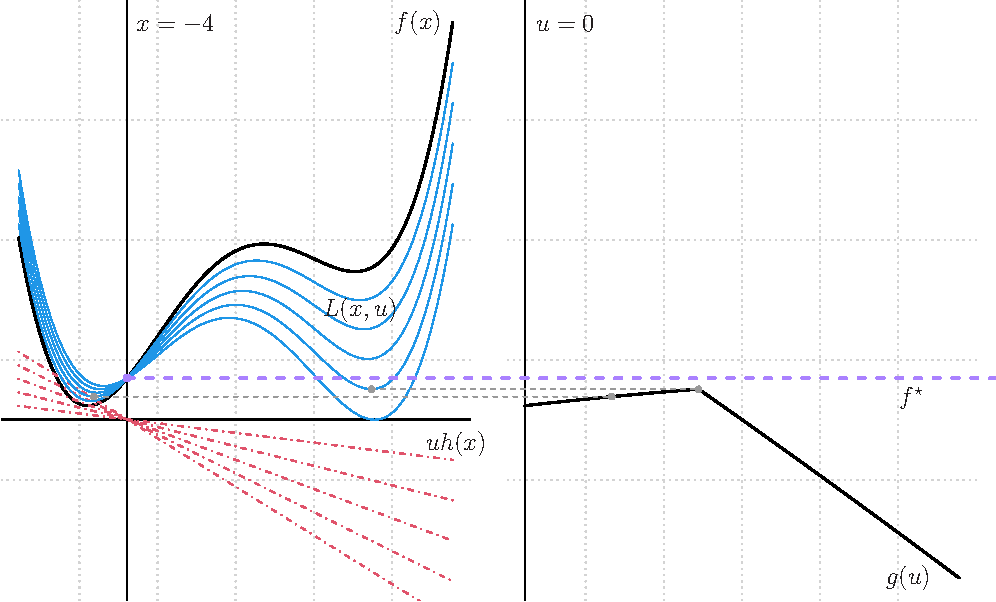
\includegraphics[width=0.89\textwidth]{fig/nonconvex_quartic.pdf}
\caption{Left: the nonconvex quartic criterion in problem
  \eqref{eq:nonconvex_quartic}, drawn as a solid curve. The dashed lines show
  $uh(x)$ as a function of $x$ for different values of the dual variable $u$,
  where $h(x) = -x-4 \leq 0$ is the inequality constraint in
  \eqref{eq:nonconvex_quartic}. The thin solid curves show the Lagrangian
  $L(x,u)$ as a function of $x$, for the same values of $u$. Right: the
  associated dual function, as in \eqref{eq:nonconvex_quartic_dual}, which at
  each $u$ is given by minimizing $L(x,u)$ over all $x$. The dashed horizontal
  line marks the optimal primal value $f^\star$. We see that weak duality
  $f^\star \geq g^\star$ holds, and the inequality is strict.}  
\label{fig:nonconvex_quartic}
\end{figure}

\section{Interpretations}
\label{sec:duality_interpretations}

In this section, we discuss some interpretations of Lagrange duality. Without
loss of generality, we will simply denote the dual variable by $u$, that is, we
drop reference to the block $v$ corresponding to the equality constraints in the
primal \eqref{eq:primal_problem}. This is possible since equality constraints
can always be rewritten as inequality constraints (each $\ell_j(x) = 0$ can be
rewritten as $\ell_j(x) \leq 0$ and $-\ell_j(x) \leq 0$). 

\paragraph{Max-min interpretation.}
\parlab{par:max_min}

Recall that, by definition \eqref{eq:dual_function}, for each $u \geq 0$,    
\[
\inf_x \, L(x,u) = g(u).
\]
Meanwhile, we also have the following symmetrical fact: for any $x$, 
\[
\sup_{u \geq 0} \, L(x,u) = f(x) + I_C(x),
\]
where $C = \{x : h_i(x) \leq 0, \, i=1,\dots,m\}$ is the primal feasible
set. To see this, note that we have the upper bound $L(x,u) \leq f(x) +
I_C(x)$ for all $x$ and $u \geq 0$. For $x \in C$, the upper bound is attained   
at $u = 0$, whereas for $x \notin C$, the upper bound is attained by sending 
$u_i \to \infty$, where $i$ is such that $h_i(x) > 0$. Therefore by the general
max-min inequality (see Exercise \ref{ex:inf_sup_rules} part d): 
\[
\underbrace{\inf_x \, \sup_{u \geq 0} \, L(x,u)}_{f^\star} \geq 
\underbrace{\sup_{u \geq 0} \, \inf_x \, L(x,u)}_{g^\star}.
\]
This is in fact precisely weak duality \eqref{eq:weak_duality}, since the 
left-hand side is \smash{$f^\star = \inf_x \{ f(x) + I_C(x) \}$} and the
right-hand side is \smash{$g^\star = \sup_{u \geq 0} \, g(u)$}. 

\paragraph{Saddle point interpretation.}

From \eqref{eq:lagrangian_bound1} and \eqref{eq:dual_function}, it follows that  
\[
f(x) \geq L(x,u) \geq g(u), \quad \text{for any primal feasible $x$ and dual
  feasible $u$}, 
\]
where by dual feasible we mean that $u \geq 0$. Suppose that $f^\star =
g^\star$, and $x^\star$ is a solution in the primal problem
\eqref{eq:primal_problem} and $u^\star$ is a solution in the dual problem
\eqref{eq:dual_problem}. Then the inequalities in the last display applied to
$x^\star,u^\star$ must be all equalities:  
\begin{equation}
\label{eq:lagrangian_equalities1}
f(x^\star) = L(x^\star, u^\star) = g(u^\star),
\end{equation}
or equivalently, 
\begin{equation}
\label{eq:lagrangian_equalities2}
\sup_{u \geq 0} \, L(x^\star, u) = L(x^\star, u^\star) = \inf_x \, L(x,
u^\star), 
\end{equation}
where used the definition of $g$ as an infimum, and the supremal representation
of $f$ established in the max-min interpretation. Observe that we can rewrite
\eqref{eq:lagrangian_equalities2} as
\index{Lagrangian function!saddle point}
\begin{equation}
\label{eq:lagrangian_saddle_point}
L(x^\star, u) \leq L(x^\star, u^\star) \leq L(x, u^\star), \quad \text{for any
  $x$ and $u \geq 0$},
\end{equation}
which says that $x^\star,u^\star$ is what is known as a \emph{saddle point} of 
the Lagrangian. 

\paragraph{Shadow price interpretation.}

Let us imagine that the primal variable $x$ in \eqref{eq:primal_problem}
represents a planning variable for a given business, and $f(x)$ is the cost 
incurred for operating according to $x$, that is, $-f(x)$ is the profit
earned. Each $h_i(x) \leq 0$ represents an operating constraint, for example, a
space constraint in the current warehouse used by the firm. (Recall, we are
dropping all equality constraints from \eqref{eq:primal_problem}, as we are  
considering the dual variable to be $u \geq 0$.)  Then in this language,
$f^\star$ is the minimal cost (maximum profit) when the firm operates according
to an optimal plan $x^\star$. 

The Lagrangian $L(x,u)$ in this context has the following interpretation. The
business is allowed to break the operating constraints, provided they pay
appropriately for violations. Each component $u_i \geq 0$ of the dual variable
corresponds to a price per unit violation of the constraint $h_i(x) \leq 0$,
that is, $u_i h_i(x)$ represents the cost to the business for violating the
$i\th$ constraint; likewise, $-u_i h_i(x)$ is the profit to the firm for slack
in the $i\th$ constraint. For example, if the firm needs more space, then they
can rent new warehouse space at a price per unit of $u_i$; and if they have
leftover space in their current warehouse, then they can rent it out at the same 
price. The value of the Lagrangian $L(x,u)$ thus represents the total cost
incurred when operating according to $x$, with prices according to $u$. The dual  
variable $u$ is often called the vector of \emph{shadow prices} in this
context. 
\index{Lagrangian function!shadow prices}

Weak duality \eqref{eq:weak_duality} now translates into the the following
statement: the optimal cost $g^\star$ when the firm is allowed to violate
constraints and pay accordingly is at most the optimal cost $f^\star$ when they
must respect the constraints, even at the worst-case prices. Moreover, if indeed
$f^\star = g^\star$, and $u^\star$ is a dual solution, then $u^\star$ represents
a set of prices for which there is no advantage to violating the constraints
versus respecting them.  

\section{Duality gap}

In different interpretations in the last section, we discussed the case when
primal and dual optimal values match,   
\index{strong duality}
\begin{equation}
\label{eq:strong_duality}
f^\star = g^\star,
\end{equation}
which is a condition we call \emph{strong duality}. To be clear, unlike weak
duality \eqref{eq:weak_duality}, strong duality is \emph{not} guaranteed to hold
in general, for any given primal problem \eqref{eq:primal_problem} and its dual  
\eqref{eq:dual_problem}. (Recall, the example in Figure
\ref{fig:nonconvex_quartic} demonstrated a failure of strong duality for problem
\eqref{eq:nonconvex_quartic}.) However, it does hold for ``most'' convex
optimization problems, as the next section makes precise. 

A related concept, for primal feasible $x$ and dual feasible $u,v$, is the
quantity  
\index{duality gap}
\begin{equation}
\label{eq:duality_gap}
f(x) - g(u,v) \geq 0,
\end{equation}
which is called the \emph{duality gap} at $x,u,v$. Note that strong duality the
case in which the duality gap is zero at a primal solution $x^\star$ and dual
solution $u^\star, v^\star$ (assuming solutions exist, that is, assuming the
optimal values are achieved).  

Though it is a simple concept, the duality gap is a powerful tool, as the next
result shows.

\begin{Theorem}
\label{thm:duality_gap}
For any primal problem \eqref{eq:primal_problem} and its dual
\eqref{eq:dual_problem}, and any primal feasible $x$ and dual feasible $u,v$,  
the following holds.  

\begin{enumerate}[label=(\roman*)]
\item If the duality gap at $x,u,v$ equals $\epsilon \geq 0$, then $f(x) -
  f^\star \leq \epsilon$, and $g^\star - g(u,v) \leq \epsilon$.  

\item If the duality gap at $x,u,v$ is zero, then $x$ is primal optimal and
  $u,v$ are dual optimal. 
\end{enumerate}
\end{Theorem}

The proof of the theorem is straightforward. If $f(x) - g(u,v) \leq \epsilon$, 
then by virtue of the fact that $f(x) \geq f^\star \geq g^\star \geq g(u,v)$, we
conclude that $f(x) - f^\star \leq \epsilon$ and $g^\star - g(u,v) \leq
\epsilon$, and this proves part (i). Meanwhile, part (ii) simply elucidates the  
special case with $\epsilon = 0$.

This theorem has numerous important implications, both in practice and in 
theory. For example, iterative algorithms which operate on the primal and the
dual simultaneously will be able to use the duality gap as a stopping criterion, 
and in doing so, will stop with a suboptimality guarantee on the primal and the 
dual criteria, by Theorem \ref{thm:duality_gap} part (i).  

As another example, Theorem \ref{thm:duality_gap} part (ii) can be used to
derive a converse of the saddle point property of the last section. There we
proved that if strong duality holds, and $x^\star,u^\star$ are primal and 
solutions, respectively (assuming no equality constraints, without loss of
generality), then $x^\star, u^\star$ is a saddle point of the Lagrangian, as in
\eqref{eq:lagrangian_saddle_point}. Conversely, if the saddle point property 
\eqref{eq:lagrangian_saddle_point} holds at a pair \smash{$\bar{x}, \bar{u}$},
then tracing back to \eqref{eq:lagrangian_equalities2} and
\eqref{eq:lagrangian_equalities1} shows that \smash{$\bar{x}, \bar{u}$} achieve
zero duality gap, which implies they must be optimal. We will revisit the saddle
point perspective in Chapter \ref{sec:saddle_point_condition}.   
\index{Lagrangian function!saddle point}
 
\section{Slater's condition}
\label{sec:slater_condition}

As we have already seen (Example \ref{ex:nonconvex_quartic}), for a nonconvex 
optimization problem, strong duality \eqref{eq:strong_duality} can fail to
hold. Fortunately, strong duality holds for a broad class of convex optimization
problems, as the next theorem makes precise.  

\index{Slater's condition}
\index{strong duality}
\begin{Theorem}
\label{thm:slater_condition}
Consider the optimization problem \eqref{eq:primal_problem}, where after 
relabeling, if needed, we take $h_1, \dots, h_r$ to be inequality constraint
functions which are affine ($r = 0$ if none are affine). Assume the following.         

\begin{enumerate}[label=(\roman*)]
\item The functions $f$ and $h_i$, $i=1,\dots,m$ are convex, and $\ell_j$,
  $j=1,\dots,k$ are affine; in other words, problem \eqref{eq:primal_problem} is
  convex, and we can write its equality constraints as $Ax = b$.      

\item There exists $x \in \relint(D)$, where \smash{$D = \dom(f) \cap
    \bigcap_{i=r+1}^m \dom(h_i)$} denotes the common effective domain, such that      
  \begin{equation}
  \label{eq:slater_condition}
  h_i(x) \leq 0 \;\, \text{for all $i \leq r$}, \quad
  h_i(x) < 0 \;\, \text{for all $i > r$}, \quad Ax = b. 
  \end{equation}
\end{enumerate}

Then strong duality holds: the optimal values $f^\star$ in problem
\eqref{eq:primal_problem} and $g^\star$ in the corresponding dual problem  
\eqref{eq:dual_problem} satisfy $f^\star = g^\star$. 
\end{Theorem}

Taken together, conditions (i) and (ii) in Theorem \ref{thm:slater_condition}
are called \emph{Slater's condition}. In short, this assumes convexity along  
with a type of strict feasibility condition \eqref{eq:slater_condition};
precisely, that there exists a point $x$ (in the relative interior of the domain
$D$) which satisfies the affine equality and inequality constraints and strictly
satisfies the nonaffine inequality constraints. This strict feasibility
condition is very mild, which is why we say that strong duality holds for
``most'' convex problems. The proof of Theorem \ref{thm:slater_condition} is
based on (an intricate application of) the separating hyperplane theorem, and is
outlined in Exercises \ref{ex:convex_theorem_alternatives} and
\ref{ex:slater_condition}.    

We can demonstrate the utility of Slater's condition by revisiting LPs. An LP
\eqref{eq:lp_primal} is always a convex problem, and all of its constraints are
affine, so Slater's condition applied to \eqref{eq:lp_primal} says that strong
duality holds if \eqref{eq:lp_primal} is feasible. Moreover, one can verify
(Exercise \ref{ex:lp_dual_dual}) that the dual of the dual problem
\eqref{eq:lp_dual} is the primal problem \eqref{eq:lp_primal}. Therefore, strong
duality in problems \eqref{eq:lp_primal} and \eqref{eq:lp_dual} refer to the
same thing, and Slater's condition applied to \eqref{eq:lp_dual} shows that
strong duality also holds if \eqref{eq:lp_dual} is feasible. Next, we summarize
these conclusions.  

\index{linear program!strong duality}
\begin{Corollary}
\label{cor:slater_lp}
For an LP, strong duality holds if the primal or the dual problem is 
feasible. 
\end{Corollary}

More can be said, by more precisely characterizing what happens when only one of
the primal or the dual is infeasible; see Exercise \ref{ex:lp_slater}. Exercises
\ref{ex:lasso_dual} and \ref{ex:svm_dual} examine duality in the lasso and SVM
problems, and use Slater's condition to conclude that strong duality always
holds.        

\section{SDP duality*}
\label{sec:sdp_duality}

Consider a generic semidefinite program (SDP) of the form
\begin{equation}
\label{eq:sdp_primal}
\begin{alignedat}{2}
&\minimize_x \quad && c^\T x \\
&\st \quad && x_1 A_1 + \cdots + x_d A_d \preceq B \\  
& && Gx = h.
\end{alignedat}
\end{equation}
To construct the Lagrangian dual of \eqref{eq:sdp_primal}, we adopt our standard 
approach of treating the space of symmetric matrices as a vector space with the   
inner product $\langle X, Y \rangle = \tr(XY)$ and partial ordering $X \preceq Y
\iff Y-X \succeq 0$. Just as before, we will associate a dual variable with
each constraint that appears in our primal problem; what this means now is that
we associate a dual matrix $U$ with the inequality constraint
\smash{$\sum_{i=1}^d x_i A_i - B \preceq 0$}, and associate a dual vector $v$
with the equality constraint $Gx - h = 0$. Hence the Lagrangian is   
\[
L(x,U,v) = c^\T x + \bigg\langle U, \sum_{i=1}^d x_i A_i - B \bigg\rangle + v^\T
(Gx - h). 
\]
Now we make use of the following key fact (Exercise
\ref{ex:psd_cone_self_dual}):   
\begin{equation}
\label{eq:psd_cone_self_dual}
Y \succeq 0 \iff \text{$\tr(XY) \geq 0$ for all $X \succeq 0$}.  
\end{equation}
We will revisit \eqref{eq:psd_cone_self_dual} in Chapter \ref{sec:dual_cones},
where in the language of that chapter, we will learn that it says the positive
semidefinite cone is self dual. Note that \eqref{eq:psd_cone_self_dual} implies 
for feasible $x$ and $U \succeq 0$,
\[
\bigg\langle U, \sum_{i=1}^d x_i A_i - B \bigg\rangle = \tr \bigg[ U \bigg(
\sum_{i=1}^d x_i A_i - B \bigg) \bigg] \leq 0.
\]
In other words, we see that indeed the Lagrangian satisfies $L(x,U,v) \leq c^\T
x$, for any feasible $x$ and $U,v$ such that $U \succeq 0$, which verifies 
\eqref{eq:lagrangian_bound1} for the current setting. Proceeding as in
\eqref{eq:lagrangian_bound2}, \eqref{eq:dual_function} \eqref{eq:dual_problem},
we minimize the Lagrangian $L(x,U,v)$ over unconstrained $U,v$ to yield the dual
problem:
\index{semidefinite program!dual problem}
\begin{equation}
\label{eq:sdp_dual}
\begin{alignedat}{2}
&\maximize_{U,v} \quad && -\tr(BU) - h^\T v \\
&\st \quad && \tr(A_iU) + g_i^\T v = -c_i, \; i = 1,\dots,d \\
& && U \succeq 0.
\end{alignedat}
\end{equation}
where $g_i$, $i=1,\dots,d$ denote the columns of $G$. Note the close analogy
between \eqref{eq:sdp_dual} and the LP dual \eqref{eq:lp_dual}. For the dual of
an SDP in standard form, see Exercise \ref{ex:sdp_std_dual}. 

By construction, we have that weak duality holds, $f^\star \geq g^\star$,
between \eqref{eq:sdp_primal} and \eqref{eq:sdp_dual}, with $f^\star$ denoting 
the optimal value in \eqref{eq:sdp_primal} and $g^\star$ the optimal value in 
\eqref{eq:sdp_dual}. When does strong duality hold? For this, we need an
extension of Slater's theorem. This will be given later in Chapter
\ref{sec:conic_duality}, when we cover conic duality, and the following is a    
consequence for SDPs. 

\index{semidefinite program!strong duality}
\begin{Corollary}
\label{cor:slater_sdp}
Strong duality holds between the SDP \eqref{eq:sdp_primal} and its dual
\eqref{eq:sdp_dual} in either of the following cases. 

\begin{enumerate}[label=(\roman*)]
\item There exists $x$ such that $Gx = h$ and $x_1 A_1 + \cdots + x_d A_d 
  \prec B$.  
\item There exists $U,v$ such that $\tr(A_iU) + g_i^\T v = -c_i$, $i =
  1,\dots,d$, and $U \succ 0$. 
\end{enumerate}
\end{Corollary}

Like the result for LPs in Corollary \ref{cor:slater_lp}, the result in
Corollary \ref{cor:slater_sdp} is based on the observation that the dual of the 
dual SDP is the primal SDP (Exercise \ref{ex:sdp_dual_dual}), so to obtain
a sufficient condition for strong duality, we can apply Slater's condition to
either the primal SDP and the dual SDP. 

While the theory of duality for SDPs has many similarities to that for LPs, it is
also important to note their differences. For example, the duality gap in an SDP
can be finite and positive, which is impossible in an LP. Exercise
\ref{ex:lp_sdp_differences} explores this and related facts.     

\SkipTocEntry\section*{Chapter notes}

Linear programming was initially the focus in developing the theory of 
duality, as laid out by David Gale, Harold Kuhn, and Albert Tucker in
\cite{gale1951linear}. This grew out of John von Neumman's famous minimax 
theorem in zero-sum, two-player games, published over two decades
earlier in \cite{vonneumann1928theorie} (we return to this and related
saddle point theorems in Chapter \ref{sec:minimax_theorems}). Historical
notes, tracing through the contributions of these and other authors, can be
found in the commentary section in Chapter 11 of
\cite{rockafellar2009variational}, among other places.

Duality is given an in depth treatment in many standard references, such as
\cite{rockafellar1970convex} (Chapters 27--32), \cite{boyd2004convex} (Chapter  
5), and \cite{bertsekas2009convex} (Chapters 4, 5). These books take on
somewhat different perspectives: Rockafellar builds up duality via conjugacy
operations, Bertsekas pursues a geometric theory based on min common/max
crossing duality, whereas Boyd and Vandenberghe take a more Lagrangian-centric 
view, and present numerous interpretations and examples of dual problems. Our
presentation is inspired in large part by \cite{boyd2004convex}. What we call
Slater's condition, in Theorem \ref{thm:slater_condition}, is called
\emph{relaxed} Slater's condition by Boyd and Vandenberghe and other
authors. Slater's condition is named after \cite{slater1950lagrange}.  

The lecture notes of \cite{bental2023convex} (Chapter 3) are a rich, advanced
resource on duality. Working in a vector space endowed with conic ordering,
these authors develop a convex theorem of alternatives, dual problems, and
optimality conditions---all from first principles. Our treatment of conic 
duality, in Chapter \ref{sec:conic_duality}, is based on theirs. A consequence
of this more general conic duality theory is the strong duality result for SDPs
in Corollary \ref{cor:slater_sdp}. Exercises
\ref{ex:convex_theorem_alternatives} and \ref{ex:slater_condition} are based on
\cite{bental2023convex}.           
 
\clearpage

\begin{xcb}{Exercises}
\begin{enumerate}[label=\thechapter.\arabic*]
\settowidth{\leftmargini}{0.00.\hskip\labelsep}
\index{linear program!dual problem}
\index{linear program!standard form}
\item \label{ex:lp_std_dual}
  Consider the standard form LP,
  \begin{alignat*}{2}
  &\minimize_x \quad && c^\T x \\
  &\st && Ax = b \\
  & && x \geq 0.
  \end{alignat*}
  Prove that its dual problem is 
%  \label{eq:lp_std_dual}
  \begin{alignat*}{2}
  &\maximize_{u,v} \quad && b^\T v \\
  &\st && A^\T v + u = c \\
  & && u \geq 0.
  \end{alignat*}

\index{quadratic program!dual problem}
\index{quadratic program!standard form}
\item \label{ex:qp_std_dual} 
  Consider the standard form QP,
  \begin{alignat*}{2}
  &\minimize_x \quad && \frac{1}{2} x^\T Q x + c^\T x \\
  &\st && Ax = b \\
  & && x \geq 0,
  \end{alignat*}
  with $Q \succ 0$. Prove that its dual problem is
%  \label{eq:lp_std_dual}
  \begin{alignat*}{2}
  &\maximize_{u,v} \quad && -\frac{1}{2} (c - A^\T v - u)^\T Q^{-1} (c - A^\T v
  - u) + b^\T v \\
  &\st && A^\T v + u = c \\
  & && u \geq 0.
  \end{alignat*}

\index{quadratic program!dual problem}
\item \label{ex:qp_psd_dual} 
  Consider the QP in \eqref{eq:qp_primal} but now assume that $Q \succeq
  0$. Prove that its dual is as claimed in \eqref{eq:qp_psd_dual}. Hint: take
  the gradient of the Lagrangian with respect to $x$, then set it equal to zero
  and rearrange to yield $Qx = -(c + A^\T u + G^\T v)$. When does this have a  
  solution? When this does not have a solution, what does that mean about the 
  infimum of the Lagrangian over $x$?   

\item \label{ex:nonconvex_quartic}
  We derive the dual for the nonconvex quartic minimization
  \eqref{eq:nonconvex_quartic}, as claimed in Example
  \ref{xa:nonconvex_quartic}. First show that taking the derivative of the
  Lagrangian with respect to $x$ and setting it equal to zero leads to
  \[
  x^3 - 25x + 25 - \frac{25}{2} u = 0.
  \]
  This is called a \emph{depressed} cubic equation, since it does not have any 
  term involving $x^2$. Show that Cardano's formula, for the roots of a
  depressed cubic, yields the three roots $x = R_j(u)$, $j = 1,2,3,\dots$ as
  defined in the example. Then argue that the dual function $g$ in 
  \eqref{eq:nonconvex_quartic_dual} can be obtained by taking the minimum value
  of the (real part of the) Lagrangian over these roots. 

\item The transportation problem from Example \parref{xa:transportation}   
  offers an intuitive example of LP duality. In this setting, recall, we have a
  per unit transportation cost $c_{ij}$ from location $i$ to $j$, a supply $s_i$
  at $i$, and a demand $d_j$ at $j$. The problem is to minimize the total
  transportation cost:  
  \begin{alignat*}{2}
  &\minimize_x \quad && \sum_{i=1}^m \sum_{j=1}^n c_{ij} x_{ij} \\ 
  &\st \quad && \sum_{j=1}^n x_{ij} = s_i, \; i=1,\dots,m \\
  & && \sum_{i=1}^m x_{ij} = d_j, \; j=1,\dots,n \\
  & && x \geq 0.
  \end{alignat*}
  Prove that its dual is (equivalent to, after reparametrization):    
  \begin{alignat*}{2}
  &\maximize_{u,v} \quad && \sum_{i=1}^m u_i s_i + \sum_{j=1}^n v_j d_j \\  
  &\st \quad && u_i + v_i \leq c_{ij}, \; i=1,\dots,m, \; j=1,\dots,n,
  \end{alignat*}
  which is sometimes referred to as the \emph{shipper's problem}. The
  interpretation is as follows. A shipper puts forth a proposal to charge $u_i$
  to load each unit from location $i$ and $v_j$ to unload each unit from
  location $j$. The shipper will try to maximize their profit, but must not
  charge more to ship from $i$ to $j$ than the given cost $c_{ij}$. By strong
  duality, a clever shipper (with dual optimal prices) will make exactly as much
  as the cheapest possible transportation cost.    
 
\item \label{ex:lp_dual_dual}
  To form the dual of \eqref{eq:lp_dual}, first convert it to a minimization
  problem by negating its criterion and rewrite the equality constraint as
  $-A^\T u - G^\T v = c$. Then simply pursue the usual steps in Lagrangian
  duality, as in Chapter \ref{sec:lagrangian_duality}. Show that this gives       
  \begin{alignat*}{2}
  &\maximize_{x,y} \quad && -c^\T x \\ 
  &\st &&  Ax + y = b \\
  & && Gx = h \\
  & && y \geq 0.
  \end{alignat*}
  After eliminating $y$ and negating the criterion to convert this to a
  minimization problem, show that we arrive back at \eqref{eq:lp_primal}.  

\index{linear program!strong duality}
\item \label{ex:lp_slater}
  Prove the following refinement of Corollary \ref{cor:slater_lp} for LPs. We
  use $f^\star, g^\star$ for the optimal values in \eqref{eq:lp_primal},
  \eqref{eq:lp_dual} respectively. 

\begin{enumerate}[label=\alph*.]
\item If both the primal \eqref{eq:lp_primal} and dual \eqref{eq:lp_dual} are
  infeasible, then strong duality fails.

\item If either the primal \eqref{eq:lp_primal} or dual \eqref{eq:lp_dual} are
  feasible, then strong duality holds.

\item If the primal \eqref{eq:lp_primal} is feasible, then $f^\star > -\infty$ 
  if and only if the dual \eqref{eq:lp_dual} is feasible.   

\item If the dual \eqref{eq:lp_dual} is feasible, then $g^\star < \infty$ if and
  only if the primal \eqref{eq:lp_primal} is feasible.     
\end{enumerate}

\item \label{ex:lasso_dual}
  Consider the lasso problem, for a response vector $y \in \R^n$ and feature   
  matrix $X \in \R^{n \times d}$, 
  \[
  \minimize_\beta \quad \frac{1}{2} \|y - X \beta\|_2^2 + \lambda \|\beta\|_1. 
  \]
  To apply Lagrangian duality, we introduce (auxiliary) constraints, rewriting
  this as    
  \begin{equation}
  \label{eq:lasso_primal}
  \minimize_{\beta,z} \quad \frac{1}{2} \|y - z\|_2^2 + \lambda \|\beta\|_1  
  \quad \st \quad z = X \beta.
  \end{equation}

\begin{enumerate}[label=\alph*.]
\item Show that the dual of \eqref{eq:lasso_primal} is (equivalent to)
  \index{lasso!dual problem} 
  \begin{equation}
  \label{eq:lasso_dual}
  \maximize_u \quad -\frac{1}{2} \|y - u\|_2^2 + \frac{1}{2} \|y\|_2^2 \quad \st
  \quad \|X^\T u\|_\infty \leq \lambda.
  \end{equation}

\item Use Slater's condition to show that strong duality always holds between 
  \eqref{eq:lasso_primal}, \eqref{eq:lasso_dual}.  
\end{enumerate}

\item \label{ex:svm_dual}
  Consider the SVM problem, for labels $y_i \in \{ -1, 1\}$ and features $x_i
  \in \R^d$, $i=1,\dots,n$,       
  \begin{equation}
  \label{eq:svm_primal}
  \begin{alignedat}{2}
  &\minimize_{\beta_0,\beta,\xi} \quad
  && \frac{1}{2} \|\beta\|_2^2 + C \sum_{i=1}^n \xi_i \\ 
  &\st \quad && y_i (\beta_0 + x_i^\T \beta) \geq 1-\xi_i, \;  i=1,\dots,n \\ 
  & && \xi \geq 0.
  \end{alignedat}
  \end{equation}

\begin{enumerate}[label=\alph*.]
\item Let $y \in \R^n$ denote the label vector and $X \in \R^{n \times d}$ the
  feature matrix (whose $i\th$ row is $x_i^\T$), and define \smash{$\tilde{X} =
    \diag(y) X$}. Show that the dual of \eqref{eq:svm_primal} is (equivalent to)      
  \index{support vector machine!dual problem} 
  \begin{equation}
  \label{eq:svm_dual}
  \begin{alignedat}{2}
  &\maximize_w \quad &&- \frac{1}{2} w^\T \tilde{X} \tilde{X}^\T w + \one^\T w \\ 
  &\st \quad && 0 \leq w \leq C \one \\
  & && y^\T w = 0.
  \end{alignedat}
  \end{equation}

\item Use Slater's condition to show that strong duality always holds between   
  \eqref{eq:svm_primal}, \eqref{eq:svm_dual}.  
\end{enumerate}

\item \label{ex:farkas_variations}
  We will examine a couple of variations on Farkas' lemma, the second of which 
  will be critical for proving the convex theorem of alternatives in the next
  exercise.      

\begin{enumerate}[label=\alph*.]
\item Given $A \in \R^{k \times d}$ and $b \in \R^k$, consider two statements: 
  \begin{itemize}
  \item for all $x \in \R^d$, it holds that $Ax \leq 0 \implies a^\T x \leq 0$;  
  \item there exists $\mu \in \R^k$ such that $\mu \geq 0$ and $A^\T \mu = 
    a$.
  \end{itemize}
  Prove that these are equivalent statements. Hint: showing that the second  
  implies the first is straightforward. To prove the other direction, apply
  Farkas' lemma, Exercise \ref{ex:farkas}, with $A,b$ replaced by $-A^\T, -a$,
  respectively.        

\item Given $A \in \R^{k \times d}$, $b \in \R^k$, $g \in \R^d$, and $h \in \R$,
  where $b \geq 0$, consider two statements:  
  \begin{itemize}
  \item for all $x \in \R^d$, it holds that $Ax \leq b \implies g^\T x \leq h$;  
  \item there exists $\mu \in \R^k$ such that $\mu \geq 0$ and $\mu^\T (Ax - b) 
    \geq g^\T x - h$ for all $x \in \R^d$.
  \end{itemize}
  Prove that these are equivalent statements. Hint: as before, showing the
  second implies the first is straightforward. For the other direction, start by
  defining 
  \[
  C = \bigg\{ \begin{bmatrix} A \\ -g^\T \end{bmatrix} x + \begin{bmatrix} u \\     
    v \end{bmatrix} : x \in \R^d, \, u \in \R^k_+, \, v > 0 \bigg\} 
  \quad \text{and} \quad D = \bigg\{ \begin{bmatrix} b \\ -h \end{bmatrix} 
  \bigg\},
  \] 
  and apply the separating hyperplane theorem, Theorem
  \ref{thm:separating_hyperplane}, to show that there exists a nonzero vector
  $(s,t) \in \R^d \times \R$ such that 
  \[
  s^\T (Ax - b) \geq t (g^\T x - h), \quad \text{for all $x \in \R^d$}.
  \]
  Argue that $A^\T s = ts$, $s \geq 0$, and $t \geq 0$; otherwise the claimed
  separation is not possible. Further, argue that $\tau > 0$; otherwise it
  follows that $A^\T s = 0$ and $b^\T s = 0$, which---after reparametrizing the  
  original space from $\R^k$ to $\col([A \; b])$, if needed---implies that $s = 
  0$. Thus, with $t > 0$, define $\mu = s/t$ in order to prove the desired
  conclusion.           
\end{enumerate}

\item \label{ex:convex_theorem_alternatives}
  Given functions $f$, $h_i$, $i=1,\dots,m$, and $\ell_j$, $j=1,\dots,k$,
  consider two feasibility problems:
  \begin{align}
  \label{eq:feasibility_problem1}
  &\begin{alignedat}{2}  
  &\find \quad && x \\ 
  &\st \quad && f(x) < c \\
  & && h_i(x) \leq 0, \; i = 1,\dots,m \\
  & && \ell_j(x) = 0, \; j = 1,\dots,k,
  \end{alignedat} \\[10pt]
  \label{eq:feasibility_problem2}
  &\begin{alignedat}{2}  
  &\find \quad && u,v \\ 
  &\st \quad && \inf_x \, \bigg\{ f(x) + \sum_{i=1}^m u_i h_i(x) + \sum_{j=1}^k 
  v_j \ell_j(x) \bigg\} \geq c \\
  & && u \geq 0.
  \end{alignedat}
  \end{align}
  The value of $c$ here is fixed and arbitrary. Following Theorem
  3.2.1 in \cite{bental2023convex}, we will prove what these authors call the 
  \emph{convex theorem of alternatives}, which says that under conditions (i)
  and (ii) in Theorem \ref{thm:slater_condition}, problem
  \eqref{eq:feasibility_problem1} is feasible if and only if
  \eqref{eq:feasibility_problem2} is infeasible.           
  
\begin{enumerate}[label=\alph*.]
\item Assume that problem \eqref{eq:feasibility_problem1} is feasible. Prove
  that \eqref{eq:feasibility_problem2} is infeasible. Hint: argue that there
  exists $x$ such that \smash{$f(x) +\sum_{i=1}^m u_i h_i(x) + \sum_{j=1}^k  v_j
    \ell_j(x) < c$}, for any $u \geq 0$ and any $v$. Note that nothing about
  this direction of the argument requires Slater's condition.   
  
\item The other direction---that infeasibility of problem
  \eqref{eq:feasibility_problem1} implies feasibility of
  \eqref{eq:feasibility_problem2}---is considerably more involved, and we will
  prove this in several steps. To simplify notation, we will assume without a
  loss of generality that $c = 0$, and that $x = 0$ satisfies condition (ii) in
  Theorem \ref{thm:slater_condition}. Moreover, for the remainder of this proof,
  we will:    
  \begin{itemize}  
  \item redefine $A,b$ such that $Ax \leq b$ represents the affine inequality
    constraints in \eqref{eq:feasibility_problem1} (originally written as
    $h_1(x) \leq 0, \dots, h_r(x) \leq 0, \pm\ell_1(x) \leq 0, \dots,
    \pm\ell_k(x) \leq 0$), then relabel the corresponding dual variable as $v
    \geq 0$; 
  \item redefine $h$ such that $h(x) \leq 0$ denotes the nonaffine inequality
    constraints in \eqref{eq:feasibility_problem1} (originally written as
    $h_{r+1}(x) \leq 0, \dots, h_m(x) \leq 0$), then relabel the corresponding
    dual variable as $u \geq 0$.
  \end{itemize}
  We will maintain $m,k$ for the dimensions of $u,v$, respectively. Now define
  the sets     
  \begin{align*}
  S &= \Big\{ (t_0, t_1) \in \R \times \R^m : t_0 < 0, \, t_1 \leq 0 \Big\}, \\  
  T &= \Big\{ (t_0, t_1) \in \R \times \R^m : \text{there exists $x$ such that
      $f(x) \leq t_0$, $h(x) \leq t_1$, and $Ax \leq b$} \Big\}. 
  \end{align*}
  Assume that \eqref{eq:feasibility_problem1} is infeasible. Prove that there
  exists a nonzero vector $a = (a_0, a_1) \in \R \times \R^m$ such that 
  \[
  \inf_{t \in T} \, a^\T t \geq 0.  
  \]
  Hint: apply the separating hyperplane theorem, Theorem
  \ref{thm:separating_hyperplane}, to $S,T$. Then argue that we must have $a
  \geq 0$ and $b = 0$ in the definition of the supporting hyperplane. 

\item Prove that $a_0 > 0$. Hint: assume in order to achieve a contradiction 
  that $a_0 = 0$. Then use $(f(0), h(0)) \in T$, and the fact that $x = 0$
  satisfies condition (ii) in Theorem \ref{thm:slater_condition}, by assumption,
  to conclude $a_1 = 0$.
\item Define $\alpha = a_1 / a_0 \in \R^m$, and  
  \[
  F(x) = f(x) + \alpha^\T h(x),
  \]
  where $h(x) = (h_1(x), \dots, h_m(x))$. Noting that $\alpha \geq 0$ (since
  $a_0 > 0$ and $a_1 \geq 0$), prove
  \[
 \text{for all $x$}, \quad Ax \leq b \implies F(x) \geq 0.
  \]
  Hint: for any $Ax \leq b$, we have $(f(x), h(x)) \in T$, so that $a^\T x \geq
  0$.

\item In what remains, we seek to show that there exists $\beta \in \R^k$ such
  that $\beta \geq 0$ and  
  \begin{equation}
  \label{eq:feasibility_problem3}
  F(x) + \beta^\T (Ax - b) \geq 0, \quad \text{for all $x$}. 
  \end{equation}
  Notice that this would complete the proof as it would verify that 
  \eqref{eq:feasibility_problem2} is feasible, with $u = \alpha$ and $v = \beta$
  (recall that we have relabeled the constraint system and taken $c =
  0$). Towards verifying the existence of such a vector $\beta$, define the sets   
  \begin{align*}
  C &= \Big\{ (x, z) \in \R^d \times \R : Ax \leq b, \, z < 0 \Big\}, \\   
  D &= \Big\{ (x, z) \in \R^d \times \R : F(x) \leq z \Big\}. 
  \end{align*}
  Prove that there exists a nonzero vector $(w, \eta) \in \R^d \times \R$ such
  that  
  \[
  \sup \Big\{ w^\T x + \eta z : Ax \leq b, \, z < 0 \Big\} \leq \inf \Big\{ w^\T
  x + \eta z : F(x) \leq z \Big\}. 
  \]
  Hint: apply the separating hyperplane theorem again, this time to $C,D$.

\item Argue that $\eta \geq 0$, so that 
  \[
  \sup \Big\{ w^\T x : Ax \leq b \Big\} \leq \inf \Big\{ w^\T x + \eta F(x) : x
  \in \R^d \Big\}.
  \]

\item Argue further that $\eta > 0$, so that by defining $\beta = w / z$, we
  have  
  \[
  \sup \Big\{ \beta^\T x : Ax \leq b \Big\} \leq \inf \Big\{ \beta^\T x + F(x) :
  x \in \R^d \Big\}.
  \]
  Hint: assume for the sake of contradiction that $\eta = 0$. Then, as $b \geq
  0$ (implied by our assumption that the origin $x = 0$ satisfies $Ax \leq b$),
  the left-hand side in the display from part f is at least zero, thus $w^\T x
  \geq 0$ for all $x$, which can only happen if $w = 0$.   

\item Let $\theta = \sup \, \{\beta^\T x : Ax \leq b\}$. Then $Ax \leq b
  \implies \beta^\T x \leq \theta$, hence by Exercise \ref{ex:farkas_variations} 
  part b, there exists a vector $\mu \geq 0$ such that $\mu^\T (Ax - b) \geq
  \beta^\T x - \theta$ for all $x$. Use this and part g to establish
  \eqref{eq:feasibility_problem3} and complete the proof. 
\end{enumerate}

\index{Slater's condition}
\item \label{ex:slater_condition}
  In this exercise, we prove Slater's condition for strong duality, in Theorem 
  \ref{thm:slater_condition}. Let $f^\star, g^\star$ be the optimal values in 
  \eqref{eq:primal_problem} and \eqref{eq:dual_problem}, respectively. Notice
  that if $f^\star = -\infty$, then the desired conclusion $f^\star = g^\star$
  is already implied by weak duality \eqref{eq:weak_duality}. Hence, assume that 
  $f^\star > -\infty$. Use the result in Exercise
  \ref{ex:convex_theorem_alternatives} to prove $f^\star = g^\star$. Hint: set
  $c = f^\star$.  

\item \label{ex:psd_cone_self_dual}
  We will prove \eqref{eq:psd_cone_self_dual}. 

\begin{enumerate}[label=\alph*.]
\item If $\tr(XY) \geq 0$ for all $X \in \SS_+^d$, then show that $Y \in
  \SS_+^d$. Hint: consider $X = a a^\T$ for an arbitrary vector $a \in \R^d$.  

\item If $Y \in \SS_+^d$, then show $\tr(XY) \geq 0$ for all $X \in
  \SS_+^d$. Hint: for $X \in \SS_+^d$, prove that we can always write \smash{$X
    = \sum_{i=1}^d x_i x_i^\T$} for vectors $x_i \in \R^d$, $i = 1,\dots,d$. 
\end{enumerate}

\index{semidefinite program!dual problem}
\index{semidefinite program!standard form}
\item \label{ex:sdp_std_dual} 
  Consider the standard form SDP,
  \begin{alignat*}{2}
  &\minimize_X \quad && \langle C, X \rangle \\
  &\st && \langle A_i, X \rangle = b_i, \; i=1,\dots,m \\
  & && X \succeq 0.
  \end{alignat*}
  Prove that its dual problem is 
  \begin{alignat*}{2}
  &\maximize_{U,v} \quad && b^\T v \\
  &\st && v_1 A_1 + \cdots v_m A_m + U = C \\
  & && U \succeq 0.
  \end{alignat*}

\item \label{ex:sdp_dual_dual}
  To form the dual of \eqref{eq:sdp_dual}, first convert it to a minimization
  problem by negating its criterion and rewrite the equality constraints as
  $-\tr(A_iU) - g_i^\T v = c_i$, $i = 1,\dots,d$. Then simply follow the usual
  steps in SDP (Lagrangian) duality, as in Chapter \ref{sec:sdp_duality}. Show
  that this gives    
  \begin{alignat*}{2}
  &\maximize_{x,Y} \quad && -c^\T x \\ 
  &\st && x_1 A_1 + \cdots + x_d A_d + Y = B \\
  & && Gx = h \\
  & && Y \succeq 0.
  \end{alignat*}
  After eliminating $Y$ and negating the criterion to convert this to a
  minimization problem, show that we arrive back at \eqref{eq:sdp_primal}.  

\item \label{ex:lp_sdp_differences}
  LPs and SDPs have several notable differences. First, we can note a difference
  in existence of solutions:
  \begin{itemize}
  \item for an LP, a solution exists whenever its optimal criterion value is
    finite (Corollary \ref{cor:weierstrass_convex_constrained}, which applies
    because for a finite optimal value, the criterion and constraint set cannot
    share a ``proper'' direction of recession along which the criterion is
    nonconstant and the constraint set nonlinear);     
  \item for an SDP, a solution can fail to exist even if the optimal value is
    finite (Exercise \ref{ex:sdp_no_solution}).   
  \end{itemize}
  Moreover, there are notable differences in duality-based perspectives for
  existence of solutions and duality theory more broadly, as we explore in the
  parts below. 

\begin{enumerate}[label=\alph*.]
\item For an SDP \eqref{eq:sdp_primal} that satisfies condition (i) in Corollary 
  \ref{thm:slater_conic}, prove that $f^\star > -\infty$ if and only if the dual 
  \eqref{eq:sdp_primal} is feasible, in which case a dual solution exists. Hint:
  apply the general Slater condition from Theorem \ref{thm:slater_conic}.   

\item Similarly, for an SDP whose dual \eqref{eq:sdp_dual} satisfies condition
  (ii) in Corollary \ref{thm:slater_conic}, prove that $g^\star < \infty$ if and
  only if the primal \eqref{eq:sdp_primal} is feasible, in which case a primal
  solution exists. Hint: again use the general Slater condition from Theorem  
  \ref{thm:slater_conic}, now on the dual. 

\item The above results for SDPs can be compared to what is known for LPs, in
  Exercise \ref{ex:lp_slater} parts c and d, where the conclusion is that a
  finite optimal criterion value implies \emph{both} primal and dual LP 
  solutions exist. Show that the statements above, in parts a and b of this
  exercise, cannot be sharpened in general for SDPs by studying the example        
  \begin{alignat*}{2}
   &\minimize_x \quad && x_1 \\
   &\st \quad && 
   \begin{bmatrix}
   x_1 & 1 \\
   1 & x_2 
 \end{bmatrix} \succeq 0.  
  \end{alignat*}
  Show that the primal optimal value is unattained (primal solution does not
  exist), but the dual optimal value is attained (dual solution exists), and
  equals the primal optimal value. Explain why this example does not violate
  parts a and b above. 

\item Show that for an LP, the duality gap $f^\star - g^\star$ can only ever be
  $0$ or $+\infty$. Hint: parts a and b of Exercise \ref{ex:lp_slater}. 

\item Show that for an SDP, the duality gap $f^\star - g^\star$ can be positive
  and finite, by studying the example 
  \begin{alignat*}{2}
   &\minimize_x \quad && x_2 \\
   &\st \quad && 
   \begin{bmatrix}
   x_2 & 0 & 0 \\
   0 & x_1 & x_2 \\
   0 & x_2 & 0 
 \end{bmatrix} \preceq  
 \begin{bmatrix}
  \alpha & 0 & 0 \\
  0 & 0 & 0 \\
  0 & 0 & 0 
 \end{bmatrix}.
  \end{alignat*}
  for arbitrary $\alpha > 0$. Compute the primal optimal value, then compute the
  dual optimal value, to conclude that the duality gap is $\alpha$. Explain why 
  this example does not violate Theorem \ref{thm:slater_conic}.  Note: this
  example is taken from \cite{ramana1997exact}, who in turn credits
  \cite{vandenberghe1996semidefinite} for a related example.  
\end{enumerate}
\end{enumerate}
\end{xcb}

\chapter{Karush-Kuhn-Tucker conditions}
\label{chap:kkt_conditions}

\section{Saddle point condition}
\label{sec:saddle_point_condition}

In this chapter, we will explore conditions which characterize solutions in
constrained optimization problems, the most well-known being a set of conditions
known as the Karush-Kuhn-Tucker (KKT) conditions. This flows naturally from our 
study of Lagrange duality in the last chapter. In fact, the last chapter already
established a critical relationship between primal and dual solutions and what
are known as saddle points of the Lagrangian. These arguments were given in 
passing, and here we revisit them, as they will lay the foundation for the KKT 
conditions, which we cover next.           

As in the last chapter, consider a primal problem
\begin{equation}
\label{eq:primal_problem2}
\begin{alignedat}{2}
&\minimize_x \quad && f(x) \\
&\st \quad && h_i(x) \leq 0, \; i=1,\dots,m \\ 
& && \ell_j(x) = 0, \; j=1,\dots,k,
\end{alignedat}
\end{equation}
whose associated Lagrangian and dual function are
\begin{align*}
L(x,u,v) &= f(x) + \sum_{i=1}^m u_i h_i(x) + \sum_{j=1}^k v_j \ell_j(x), \\ 
g(u,v) &= \inf_x \, L(x,u,v), 
\end{align*}
and whose associated dual problem is 
\begin{equation}
\label{eq:dual_problem2}
\maximize_{u,v} \quad g(u,v) \quad \st \quad u \geq 0.
\end{equation}
We do not assume that \eqref{eq:primal_problem2} is convex, though recall, the 
dual problem \eqref{eq:dual_problem2} is always convex. In general, we say that
a triplet \smash{$\bar{x}, \bar{u}, \bar{v}$} is a \emph{saddle point} of the
Lagrangian if  
\index{Lagrangian function!saddle point} 
\begin{equation}
\label{eq:lagrangian_saddle_point2}
L(\bar{x}, u, v) \leq L(\bar{x}, \bar{u}, \bar{v}) \leq L(x, \bar{u}, \bar{v}),
\quad \text{for any $x$ and any $u \geq 0, \, v$}.
\end{equation}
In other words, starting at \smash{$\bar{x}, \bar{u}, \bar{v}$}, the condition
says: if we move the primal variable away from \smash{$\bar{x}$} then $L$ can
only increase; if we move the dual variables away from \smash{$\bar{u},
  \bar{v}$}, then $L$ can only decrease.    

The following is a useful characterization of primal and dual solutions via
saddle points.  

\begin{Theorem}
\label{thm:saddle_point_optimality}
For any primal problem \eqref{eq:primal_problem2} and its dual
\eqref{eq:dual_problem2}, and any primal feasible \smash{$\bar{x}$} and dual
feasible \smash{$\bar{u}, \bar{v}$}, the triplet \smash{$\bar{x}, \bar{u},
  \bar{v}$} is a saddle point of the Lagrangian
\eqref{eq:lagrangian_saddle_point2} if and only if \smash{$\bar{x}$} is primal
optimal, \smash{$\bar{u}, \bar{v}$} are dual optimal, and strong duality holds. 
\end{Theorem}

Though the arguments behind this result were already given in Chapter 
\ref{chap:lagrangian_duality}, it will be helpful to consolidate them here.
First, note that the saddle point condition
\eqref{eq:lagrangian_saddle_point2} has a couple of equivalent forms:
\begin{equation}
\label{eq:lagrangian_saddle_point3}
\sup_{u \geq 0, \, v} \, L(\bar{x}, u, v) = L(\bar{x}, \bar{u}, \bar{v}) =
\inf_x \, L(x, \bar{u}, \bar{v}), 
\end{equation}
as well as
\begin{equation}
\label{eq:lagrangian_saddle_point4}
f(\bar{x}) = L(\bar{x}, \bar{u}, \bar{v}) = g(\bar{u}, \bar{v}).
\end{equation}
The right-hand side in the above display is due to the definition of the dual
function $g$, whereas the left-hand side uses the representation of $f$ as a
supremum of the Lagrangian, from Property \parref{par:max_min}. To prove    
Theorem \ref{thm:saddle_point_optimality} we simply observe that 
\eqref{eq:lagrangian_saddle_point4} is equivalent to \smash{$\bar{x}, \bar{u}, 
  \bar{v}$} being primal and dual solutions with zero duality gap. 

\section{Karush-Kuhn-Tucker conditions}
\label{sec:kkt_conditions}

We say that a triplet \smash{$\bar{x}, \bar{u}, \bar{v}$} is a
\emph{Karush-Kuhn-Tucker (KKT) point} associated with the primal and 
dual pair \eqref{eq:primal_problem2} and \eqref{eq:dual_problem2} if it
satisfies the following conditions: 
\index{KKT conditions}
\begin{alignat}{2}
\label{eq:kkt_stationarity}
&0 \in \partial_x L(\bar{x}, \bar{u}, \bar{v}) \quad
&& \text{(stationarity)} \\
\label{eq:kkt_complementary_slackness} 
&\bar{u}_i h_i(\bar{x}) = 0, \; i = 1,\dots,m \quad 
&& \text{(complementary slackness)} \\
\label{eq:kkt_primal_feasibility}
&h_i(\bar{x}) \leq 0, \; i = 1,\dots,m, \; \text{and} \; 
\ell_j(\bar{x}) = 0, \; j = 1,\dots,k \quad 
&& \text{(primal feasibility)} \\ 
\label{eq:kkt_dual_feasibility}
&\bar{u}_i \geq 0, \; i = 1,\dots,m. \quad
&& \text{(dual feasibility)}
\end{alignat}
To be clear, in \eqref{eq:kkt_stationarity}, called the stationarity condition,
the subdifferential is taken with respect to the $x$ component of the
Lagrangian.  

The next result shows that the KKT conditions offer yet another equivalent
characterization of saddle point condition (together with feasibility).  

\begin{Lemma}
\label{lem:saddle_point_kkt}
For any primal feasible \smash{$\bar{x}$} and dual feasible \smash{$\bar{u}, 
  \bar{v}$}, the saddle point condition \eqref{eq:lagrangian_saddle_point2} is
equivalent to stationarity and complementary slackness,
\eqref{eq:kkt_stationarity} and \eqref{eq:kkt_complementary_slackness}.
\end{Lemma}

The proof is straightforward, if we use the equivalent form of the saddle point
condition \eqref{eq:lagrangian_saddle_point4}. The second equality in
\eqref{eq:lagrangian_saddle_point4} is equivalent to the fact that
\smash{$\bar{x}$} minimizes \smash{$L(\cdot, \bar{u}, \bar{v})$}, which is
equivalent to stationarity \eqref{eq:kkt_stationarity}. The first equality in
\eqref{eq:lagrangian_saddle_point4} is implied by complementary slackness
\eqref{eq:kkt_complementary_slackness}:
\[
L(\bar{x}, \bar{u}, \bar{v}) = f(\bar{x}) + 
\sum_{i=1}^m \underbrace{\bar{u}_i h_i(\bar{x})}_{=\,0} + 
\sum_{j=1}^k \underbrace{\bar{v}_j \ell_j(\bar{x})}_{=\,0} 
= f(\bar{x}),
\]
where we have used primal feasibility. Furthermore, the first equality in
\eqref{eq:lagrangian_saddle_point4} also implies complementary slackness: if
\smash{$f(\bar{x}) = L(\bar{x}, \bar{u}, \bar{v})$}, then (again using primal
and dual feasibility) we conclude that all summands must be zero in the middle
expression of the last display, which leads to
\eqref{eq:kkt_complementary_slackness}. This completes the proof the theorem.

Combining Theorem \ref{thm:saddle_point_optimality} and Lemma
\ref{lem:saddle_point_kkt} yields the following important result. 

\index{KKT conditions!optimality}
\begin{Theorem}
\label{thm:kkt_optimality}
For any primal problem \eqref{eq:primal_problem2} and its dual
\eqref{eq:dual_problem2}, a triplet \smash{$\bar{x}, \bar{u}, \bar{v}$}
satisfies the KKT conditions
\eqref{eq:kkt_stationarity}--\eqref{eq:kkt_dual_feasibility} if and only if 
\smash{$\bar{x}$} is primal optimal, \smash{$\bar{u}, \bar{v}$} are dual
optimal, and strong duality holds. In other words, the KKT conditions are always
sufficient for optimality, and necessary under strong duality.   
\end{Theorem}

\index{subgradient!optimality condition}
\index{Lagrange multiplier condition} 
It is worth noting that the KKT conditions generalize the subgradient optimality
condition \eqref{eq:subgradient_optimality}. That is, if problem
\eqref{eq:primal_problem2} has no constraints ($m = k = 0$), then the Lagrangian
is simply the primal criterion, $L = f$, and the only non-vacuous KKT condition
is stationarity \eqref{eq:kkt_stationarity}, which reduces to
\eqref{eq:subgradient_optimality}. Similarly, the KKT conditions generalize the
Lagrange multiplier condition \eqref{eq:lagrange_multiplier}, which can seen
either because the subgradient optimality condition does, or directly from
stationarity \eqref{eq:kkt_stationarity} with linear equality constraints of the
form $Ax = b$. 

\begin{Example}
The following examples discuss the KKT conditions for problems of interest. In
each case, the KKT conditions are necessary and sufficient for optimality, as
the problem in question is convex and strong duality holds by Slater's condition
(Theorem \ref{thm:slater_condition}). 

\begin{enumerate}[label=\alph*., ref=\alph*]
\item Consider a QP with equality constraints only, 
  \begin{alignat*}{2}
  &\minimize_x \quad && c^\T x + \frac{1}{2} x^\T Q x \\
  &\st && Ax = b,
  \end{alignat*}
  where $Q \succeq 0$. Its Lagrangian is 
  \[
  L(x,v) = c^\T x + \frac{1}{2} x^\T Q x + v^\T (Ax - b).
  \]
  Complementary slackness \eqref{eq:kkt_complementary_slackness} and dual
  feasibility \eqref{eq:kkt_dual_feasibility} are vacuous due to the lack of 
  inequality constraints. Stationarity \eqref{eq:kkt_stationarity} and primal
  feasibility \eqref{eq:kkt_primal_feasibility} are each linear equations, which
  can be assembled into one combined linear system:
  \index{Karush-Kuhn-Tucker matrix}
  \[
  \begin{bmatrix} Q & A^\T \\ A & 0 \end{bmatrix}  
  \begin{bmatrix} x \\ v \end{bmatrix} =
  \begin{bmatrix} -c \\ b \end{bmatrix}.
  \]
  The above matrix is often called the \emph{KKT matrix} associated with our
  original QP. 

\item \parlab{xa:lasso_kkt}
  Consider the lasso problem
  \begin{equation}
  \label{eq:lasso_primal2}
  \minimize_\beta \quad \frac{1}{2} \|y - X \beta\|_2^2 + \lambda \|\beta\|_1, 
  \end{equation}
  for a response vector $y \in \R^n$ and feature matrix $X \in \R^{n \times
    d}$. Since this problem has no constraints, the KKT conditions reduce to  
  stationarity (which, as discussed above, is just the subgradient optimality 
  condition):   
  \index{lasso!optimality conditions}
  \begin{equation}
  \label{eq:lasso_optimality}
  X^\T (y - X\beta) = \lambda s, \quad \text{where $s \in \partial
    \|\beta\|_1$}. 
  \end{equation}
  This condition characterizes lasso solutions. We will see later, in Chapter
  \ref{sec:lasso_structure}, that it provides a way to understand the structure
  of lasso solutions.    
  
\item \parlab{xa:svm_kkt}
  Consider the SVM problem
  \begin{equation}
  \label{eq:svm_primal2}
  \begin{alignedat}{2}
  &\minimize_{\beta_0,\beta,\xi} \quad
  && \frac{1}{2} \|\beta\|_2^2 + C \sum_{i=1}^n \xi_i \\ 
  &\st \quad && y_i (\beta_0 + x_i^\T \beta) \geq 1-\xi_i, \;  i=1,\dots,n \\ 
  & && \xi \geq 0,
  \end{alignedat}
  \end{equation}
  for labels $y_i \in \{ -1, 1\}$ and features $x_i \in \R^d$, $i=1,\dots,n$. 
  Its Lagrangian is
  \[
   L(\beta,\beta_0,\xi,\alpha,u) = 
   \frac{1}{2} \|\beta\|_2^2 + C \sum_{i=1}^n \xi_i +  \sum_{i=1}^n \alpha_i 
   \big(1-\xi_i - y_i (\beta_0 + x_i^\T \beta) \big) - u^\T \xi. 
   \]
  The stationarity condition \eqref{eq:kkt_stationarity} reads
  \index{support vector machine!optimality conditions}
  \begin{equation}
  \label{eq:svm_stationarity}
  \sum_{i=1}^n \alpha_i y_i = 0, \quad 
  \sum_{i=1}^n \alpha_i y_i x_i = \beta, \quad
  \alpha_i + u_i = C, \quad i = 1,\dots,n.
  \end{equation}
  Complementary slackness \eqref{eq:kkt_complementary_slackness} reads   
  \begin{equation}
  \label{eq:svm_complementary_slackness}
    \alpha_i \big(1-\xi_i - y_i (\beta_0 + x_i^\T \beta) \big) = 0, \quad
    u_i \xi_i = 0, \quad i=1,\dots,n. 
  \end{equation}
  Together with primal and dual feasibility, the above two conditions
  characterize SVM solutions. We will see later, in Chapter
  \ref{sec:svm_structure}, that these conditions provide a basis for
  understanding the structure of SVM solutions.   
\end{enumerate}
\end{Example}

\section{Primal-dual relationships}

For a primal-dual pair \eqref{eq:primal_problem2}, \eqref{eq:dual_problem2}
which exhibit strong duality, we know (Theorem \ref{thm:kkt_optimality}) that
the KKT conditions are necessary and sufficient for optimality. The stationarity
condition \eqref{eq:kkt_stationarity} allows us to relate primal $x^\star$ and
dual $u^\star, v^\star$ solutions. Rephrased, this condition says that 
\index{KKT conditions!primal-dual relationship}
\begin{equation}
\label{eq:kkt_stationarity2}
\text{$x^\star$ minimizes $L(\cdot, u^\star, v^\star)$}.
\end{equation}
As demonstrated in the examples that follow, we can often rearrange
\eqref{eq:kkt_stationarity2} to form a \emph{primal-dual relationship}, which is
an equation that relates primal and dual solutions. Further, if $L(\cdot,
u^\star, v^\star)$ has a unique minimizer, then this relationship uniquely
specifies $x^\star$ as a function of $u^\star, v^\star$. 

Primal-dual relationships can be useful for two main reasons. First, in the case
that it uniquely specifies the primal solution $x^\star$, a primal-dual
relationship enables us to solve the primal \eqref{eq:primal_problem2} via the
dual \eqref{eq:dual_problem2}, which is useful in practice when the latter is
easier solve than the former. Second, a primal-dual relationship can provide an
avenue for inferring properties of solutions.

\index{support vector machine!primal-dual relationship}
A clear example of this is given by SVM duality, as studied in Example
\parref{xa:svm_kkt}. The stationarity condition \eqref{eq:svm_stationarity}
immediately reveals that the primal solution \smash{$\hbeta$} can be written in
terms of the dual solution via \smash{$\hbeta = \sum_{i=1}^n \halpha_i y_i
  x_i$}. Generally, some coordinates of the dual solution will be equal to
zero, \smash{$\halpha_i = 0$}, by the nonnegativity constraint in
\eqref{eq:svm_dual}; the corresponding feature vectors $x_i$ and labels $y_i$
play no role in shaping \smash{$\hbeta$}, which determines the orientation of
the linear SVM classifier. Meanwhile, the coordinates for which
\smash{$\halpha_i \not= 0$} index what are called \emph{support points} $x_i$
and $y_i$ of the classifier; we revisit this in more detail in Chapter
\ref{sec:svm_structure}.      

For the lasso, as studied in Example \parref{xa:lasso_kkt}, the problem
\eqref{eq:lasso_primal2} has no constraints and thus no associated dual   
variables. As written, the stationarity condition \eqref{eq:lasso_optimality}
relates the primal solution to itself, and not to dual variables. In order to
make progress toward a primal-dual relationship, we can introduce auxiliary
equality constraints in the lasso problem.

\begin{Example}
As in Exercise \ref{ex:lasso_dual}, consider writing the lasso problem
\eqref{eq:lasso_primal2} as 
\[
\minimize_{\beta,z} \quad \frac{1}{2} \|y - z\|_2^2 + \lambda \|\beta\|_1  
\quad \st \quad z = X \beta.
\]
This allows us to write its Lagrangian as     
\[
L(\beta,z,u) = \frac{1}{2} \|y - z\|_2^2 + \lambda \|\beta\|_1 + u^\T (z - X
\beta).
\]
The stationarity condition \eqref{eq:kkt_stationarity} now reads
\[
z = y-u, \quad X^\T u \in \lambda \partial \|\beta\|_1.
\]
By the first equation above, as \smash{$\hat{z} = X \hbeta$} at the solution, 
we have the primal-dual relationship    
\index{lasso!primal-dual relationship}
\begin{equation}
\label{eq:lasso_primal_dual}
X \hbeta = y - \hat{u}.
\end{equation}
Any lasso solution \smash{$\hbeta$} in \eqref{eq:lasso_primal2} (which is not
necessarily unique, if $X$ has linearly dependent columns) and the dual solution 
\smash{$\hat{u}$} in \eqref{eq:lasso_dual} (which is unique since the dual
criterion is strictly concave) must together satisfy
\eqref{eq:lasso_primal_dual}. Furthermore, by straightforward rearrangement, the
dual problem \eqref{eq:lasso_dual} is equivalent to  
\index{lasso!dual problem} 
\[
\minimize_u \quad \|y - u\|_2^2 \quad \st \quad \|X^\T u\|_\infty \leq \lambda.
\]
We can hence write the dual solution as \smash{$\hat{u} = P_C(y)$}, the
projection of $y$ onto the convex set
\[
C = \{ u : \|X^\T u\|_\infty \leq \lambda \}. 
\]
From \eqref{eq:lasso_primal_dual}, we infer that \smash{$X \hbeta =
  (I-P_C)(y)$}, which is the residual from projection onto $C$. As the residual 
from projection onto a convex set is nonexpansive
\eqref{eq:projection_residual_nonexpansiveness}, writing \smash{$X 
\hbeta$}---called the lasso \emph{fitted vector} (or simply the lasso
\emph{fit})---in this form leads to the following conclusion about
smoothness. For any two response vectors $y, y' \in \R^n$ and the corresponding
lasso fitted vectors \smash{$X \hbeta(y), X \hbeta(y') \in \R^n$}, we have
\begin{equation}
\label{eq:lasso_nonexpansive}
\|X \hbeta(y) - X \hbeta(y')\|_2 \leq \|y - y'\|_2.
\end{equation}
That is, the lasso fit \smash{$X \hbeta(y)$} is Lipschitz continuous as a
function of $y$ (with Lipschitz constant $L = 1$), and therefore differentiable
almost everywhere (by Rademacher's theorem).    
\end{Example}

\section{Stationarity and convexity*}

The KKT conditions \eqref{eq:kkt_stationarity}--\eqref{eq:kkt_dual_feasibility}
do not assume anything about convexity of the primal problem
\eqref{eq:primal_problem2}. As conveyed in the theory developed above (Theorem  
\ref{thm:saddle_point_optimality}, Lemma \ref{lem:saddle_point_kkt}, Theorem
and \ref{thm:kkt_optimality}), these conditions characterize primal-dual solutions
in general optimization problems. The arguments that underlie this theory are
elementary; however, they do rely heavily on the theory of Lagrangian duality
developed in the last chapter.   

Convexity is nonetheless a centrally important consideration in most uses of the
KKT optimality conditions. For one, they are only necessary under strong
duality, which is understood to hold most generally for convex problems
(Slater's condition, Theorem \ref{thm:slater_condition}). That is, optimization
problems in which strong duality does not hold can have solutions which violate  
the KKT conditions, and if we rely on the KKT conditions to characterize
optimality in such problems, then we may miss some or all solutions entirely.        

Furthermore, the stationarity condition \eqref{eq:kkt_stationarity} has a
well-known equivalent form under convexity. This condition expresses the fact
that \smash{$\bar{x}$} minimizes the $x$ argument of the Lagrangian with the
other arguments fixed at \smash{$\bar{u}, \bar{v}$}, and it does so using the
language of subgradients. When the primal criterion function $f$ and constraint
functions $h_i$, $i=1,\dots,m$ and $\ell_j$, $j=1,\dots,k$ are each convex, and 
their domains have relative interiors with nonempty intersection, we can split
up the subgradient of the Lagrangian with respect to $x$ into a sum of
subgradients (Property \parref{par:subgradient_sum}), rewriting the stationarity
condition \eqref{eq:kkt_stationarity} as   
\begin{equation}
\label{eq:kkt_stationarity3}
0 \in \partial f(\bar{x}) + \sum_{i=1}^m \bar{u}_i \partial h_i(\bar{x}) +
\sum_{j=1}^k \bar{v}_j \partial \ell_j(\bar{x}).
\end{equation}
If in addition the primal criterion and constraint functions are each
differentiable, then subgradients reduce to gradients (Theorem
\ref{thm:subgradient_uniqueness}), and we can rewrite  
\eqref{eq:kkt_stationarity3} once more as  
\begin{equation}
\label{eq:kkt_stationarity4}
0 = \nabla f(\bar{x}) + \sum_{i=1}^m \bar{u}_i \nabla h_i(\bar{x}) +
\sum_{j=1}^k \bar{v}_j \nabla \ell_j(\bar{x}).
\end{equation}
The forms \eqref{eq:kkt_stationarity3} and especially
\eqref{eq:kkt_stationarity4} are widely-used to express stationarity in
references on the KKT optimality conditions.  

One must be careful when interpreting \eqref{eq:kkt_stationarity3} or
\eqref{eq:kkt_stationarity4} on their own, absent their connection to   
\eqref{eq:kkt_stationarity}. For general $f$, $h_i$, $i=1,\dots,m$, $\ell_j$, 
$j=1,\dots,k$, we only know (Property \parref{par:subgradient_sum}) that   
\[
\partial f(\bar{x}) + \sum_{i=1}^m \bar{u}_i \partial h_i(\bar{x}) +
\sum_{j=1}^k \bar{v}_j \partial \ell_j(\bar{x}) \subseteq \partial_x \bigg( f(x) 
+ \sum_{i=1}^m \bar{u}_i h_i(x) + \sum_{j=1}^k \bar{v}_j \partial \ell_j(x)
\bigg) \bigg|_{x = \bar{x}}, 
\]
and therefore \eqref{eq:kkt_stationarity3} implies \eqref{eq:kkt_stationarity}
but not the other way around. Meanwhile, nonconvex functions can have gradients
that are not subgradients, so \eqref{eq:kkt_stationarity4} is not even
sufficient for \eqref{eq:kkt_stationarity} in general.   

For differentiable nonconvex problems, the alternative stationarity condition
\eqref{eq:kkt_stationarity4}, combined with the other KKT conditions  
\eqref{eq:kkt_complementary_slackness}--\eqref{eq:kkt_dual_feasibility}, are 
often studied under what are known as \emph{constraint qualification (CQ)}  
conditions. (Slater's condition is an example of CQ, but there are many others.)
CQ is used to ensure that \eqref{eq:kkt_stationarity4} and
\eqref{eq:kkt_complementary_slackness}--\eqref{eq:kkt_dual_feasibility} are   
necessary for optimality. Hence \eqref{eq:kkt_stationarity4} and
\eqref{eq:kkt_complementary_slackness}--\eqref{eq:kkt_dual_feasibility} are 
sometimes called the KKT \emph{necessary} conditions in the literature on
differentiable nonconvex programming. Sufficient conditions in this setting
often involve additional second-order statements. The chapter notes provide some
further discussion. 

\section{Constrained and penalized equivalences*}

In statistics and machine learning, we often encounter penalized problems of the
form  
\begin{equation}
\label{eq:penalized_problem}
\minimize_\theta \quad \ell(\theta) + \lambda r(\theta),
\end{equation}
for a loss function $\ell$ (such as the negative log likelihood in a parametric
model), regularizer $r$ (such as a norm or seminorm), and tuning parameter
$\lambda \geq 0$. A common claim is that \eqref{eq:penalized_problem} is
equivalent to the constrained problem
\begin{equation}
\label{eq:constrained_problem}
\minimize_\theta \quad \ell(\theta) \quad \st \quad r(\theta) \leq t, 
\end{equation}
where $t \in \R$ is another tuning parameter. In what follows, we formalize this
claim using the KKT conditions. Fixing any $\lambda \geq 0$, we first show that   
any solution \smash{$\htheta$} in the penalized problem
\eqref{eq:penalized_problem} is a solution in the constrained problem 
\eqref{eq:constrained_problem}, for an appropriate choice of $t$. In
particular, we define \smash{$t = r(\htheta)$}, which we assume to be finite. We 
now simply check that \smash{$\htheta, \lambda$} satisfy the KKT conditions for  
\eqref{eq:constrained_problem}: stationarity holds because \smash{$\htheta$} 
minimizes the Lagrangian
\begin{equation}
\label{eq:constrained_lagrangian}
L(\theta, \lambda) = \ell(\theta) + \lambda (r(\theta) - t)
\end{equation}
over $\theta$; complementary slackness holds because \smash{$r(\htheta) = t$};
and primal and dual feasibility clearly hold as well. The KKT conditions being
sufficient for optimality, this implies that \smash{$\htheta$} solves
\eqref{eq:constrained_problem}.       

For the other direction: fixing any $t \in \R$, we will show that under strong
duality (or any other CQ condition that implies necessity of the KKT
conditions), any solution \smash{$\htheta$} in \eqref{eq:constrained_problem} is
a solution in \eqref{eq:penalized_problem}, for an appropriate choice of
$\lambda$. In particular, take $\lambda \geq 0$ to be any solution---assumed to
be attained and finite---in the dual of \eqref{eq:constrained_problem}. The KKT 
conditions being necessary for optimality under strong duality, we know by
stationarity that \smash{$\htheta$} must minimize $L(\theta, \lambda)$ in
\eqref{eq:constrained_lagrangian} over $\theta$, which implies it must solve    
\eqref{eq:penalized_problem}.   

We summarize the above conclusions into the following theorem.

\begin{Theorem}
For functions $\ell,r : \R^d \to [-\infty, \infty]$, and $\lambda,t \in \R$, the
penalized \eqref{eq:penalized_problem} and constrained
\eqref{eq:constrained_problem} problems admit the following equivalences.     

\begin{enumerate}[label=(\roman*)]
\item If \smash{$\htheta$} solves \eqref{eq:penalized_problem} and \smash{$t =
    r(\htheta) < \infty$}, then \smash{$\htheta$} solves
  \eqref{eq:constrained_problem}. 

\item If a constraint qualification condition holds for
  \eqref{eq:constrained_problem}, such as Slater's condition (which requires
  $\ell,r$ to be convex, and for $\{ \theta : r(\theta) < t\}$ to be nonempty),
  and if \smash{$\htheta$} solves \eqref{eq:constrained_problem} and $\lambda
  \in [0,\infty)$ solves its dual, then \smash{$\htheta$} solves
  \eqref{eq:penalized_problem}.   
\end{enumerate} 
\end{Theorem}

\SkipTocEntry\section*{Chapter notes}

What does 

Bertsekas have to say?
Rockafellar have to say?
Rockafellar and Wets have to say?

Big admission that we are using KKT to mean what others will not call KKT. They
mean 10.19 and the rest.

Describe what we mentioned in 10.4. Boyd and Van is an example of this.

What setting did Kuhn and Tucker study in their original paper? What about
Karush? 
 
Refs....

W. KARUSH (1939), Minima of Functions of Several Variables with Inequalities as
Side Constraints, M. Sc. Dissertation, Dept. of Mathematics, University of
Chicago 

H. W. KUHN and A. W. TUCKER (1951), Nonlinear programming; in
J. Neyman (Ed.), Proceedings of the Second Berkeley Symposium on Mathematical
Statistics and Probability, Univ. of California Press, Berkeley, 481-492. 

Kjeldsen, Tinne Hoff. A contextualized historical analysis of the Kuhn–Tucker
theorem in nonlinear programming: the impact of world war II. Historia
mathematica, 27(4): 331–361, 2000. 

 John (1948) 

% Ideas for advanced topics or exercises: 
% Fritz John conditions
% Invex functions
% Second-order conditions

\begin{xcb}{Exercises}
\begin{enumerate}[label=\thechapter.\arabic*]
\settowidth{\leftmargini}{00.00.\hskip\labelsep}
\item 

\item \label{ex:lasso_dantzig}
Compare these two? And how about basis pursuit?

\item graphical lasso and covariance thresholding

\item \label{ex:simplex_projection}

\end{enumerate}
\end{xcb}
\chapter{Duality correspondences}
\label{chap:duality_correspondences}

In this chapter we explore various topics which connect to our treatment of 
Lagrangian duality and the KKT conditions in the last two chapters.

\section{Dual norms}
\label{sec:dual_norms}

Given a norm $\|\cdot\|$ on $\R^d$, its \emph{dual norm} is denoted
$\|\cdot\|_*$, and defined by 
\index{dual norm}  
\begin{equation}
\label{eq:dual_norm}
\|y\|_* = \sup_{\|x\| \leq 1} \, y^\T x.
\end{equation}
It is not hard to check that the dual norm $\|\cdot\|_*$ is itself a norm on
$\R^d$, that is, it satisfies the triangle inequality, absolute homogeneity, and
positive definiteness (Exercise \ref{ex:dual_norm_check}). 

A key property to record: the dual of the dual norm is the original norm,
$\|\cdot\|_{**} = \|\cdot\|$. This is traditionally verified using the
Hahn-Banach theorem (Exercise \ref{ex:dual_norm_dual1}), but can also be
derived using the theory of Lagrangian duality (Exercise
\ref{ex:dual_norm_dual2}), or even convex conjugacy (Exercise
\ref{ex:dual_norm_dual3}). In any case (however it is proved), this fact allows 
us to write    
\begin{equation}
\label{eq:norm_dual2}
\|x\| = \sup_{\|y\|_* \leq 1} \, x^\T y.
\end{equation}

Directly from \eqref{eq:dual_norm}, we may infer that $x^\T y \leq \|x\|$ for
all $x$ and $\|y\|_* \leq 1$, or     
\index{H{\"o}lder's inequality}
\begin{equation}
\label{eq:holder_inequality}
x^\T y \leq \|x\| \|y\|_*, \quad \text{for all $x,y$}.
\end{equation}
This may be seen as a generalization of \emph{H{\"o}lder's inequality} for
$\ell_p$ norms. When does equality hold in \eqref{eq:holder_inequality}? The
representations \eqref{eq:dual_norm}, \eqref{eq:norm_dual2}, combined with the
fact about subgradients of norms in \eqref{eq:norm_subgradients}, lead to the 
following equivalent conditions (Exercise \ref{ex:dual_norm_subgradients}).     

\index{norm!subgradients}
\index{dual norm!subgradients}
\begin{Theorem}
\label{thm:dual_norm_subgradients}
For any norm $\|\cdot\|$ and its dual $\|\cdot\|_*$, and any $x \not= 0$ and $y 
\not= 0$, the following statements are equivalent:
\begin{enumerate}[label=(\roman*)]
\item $x^\T y = \|x\| \|y\|_*$;
\item $x/\|x\| \in \partial \|y\|_*$; 
\item $y/\|y\|_* \in \partial \|x\|$;
\item $x/\|x\| \in \argmax_{\|s\| \leq 1} \, y^\T s$; 
\item $y/\|y\|_* \in \argmax_{\|s\|_* \leq 1} \, x^\T s$. 
\end{enumerate}
\end{Theorem}

The next example confirms that \eqref{eq:holder_inequality} is indeed a strict 
generalization of H{\"o}lder's inequality for $\ell_p$ norms, as it shows the
dual of the $\ell_p$ norm is the $\ell_q$ norm for a conjugate pair $p,q$.      

\begin{Example}
The following are examples of dual norms for common norms, which can be verified
by direct calculation (Exercises \ref{ex:lp_norm_dual}--\ref{ex:trace_norm_dual}). 

\begin{enumerate}[label=\alph*., ref=\alph*]
\index{lp norm@$\ell_p$ norm!dual norm}
\item \parlab{xa:lp_norm_dual} 
For the $\ell_p$ norm $\|\cdot\|_p$ with $p \geq 1$, its dual norm is
$\|\cdot\|_q$ where $q$ satisfies $1/p + 1/q = 1$.  

\item \parlab{xa:scaled_euclidean_norm_dual}  
For the scaled Euclidean norm $\|\cdot\|_A$ in a given positive definite
matrix $A$, which recall is defined by \smash{$\|x\|_H = \sqrt{x^\T A x}$},
its dual norm is \smash{$\|\cdot\|_{A^{-1}}$}.  

\index{trace norm!dual norm}
\index{operator norm!dual norm}
\item \parlab{xa:trace_norm_dual}  
For the trace norm $\|\cdot\|_{\tr}$, its dual norm is the operator norm
$\|\cdot\|_{\op}$.   
\end{enumerate}
\end{Example}

Dual norms bear interesting connections to conjugacy. As already shown in
Example \parref{xa:norm_conjugate}, the conjugate of a norm is the
characteristic function of the dual norm unit ball:  
\index{norm!conjugate}
\begin{equation}
\label{eq:norm_conjugate}
(\|\cdot\|)^* = I_{\{u : \|u\|_* \leq 1\}}.
\end{equation}
Meanwhile, an arguably even simpler relationship holds for the squared norm; the
convex conjugate of one half times a norm squared is one half times its dual
norm squared (Exercise \ref{ex:norm_squared_conjugate}):       
\begin{equation}
\label{eq:norm_squared_conjugate}
\Big( \frac{1}{2} \|\cdot\|^2 \Big)^{\hspace{-2pt}*} = \frac{1}{2}
\|\cdot\|_*^2.   
\end{equation}
These facts are especially useful in the context of Fenchel duality, which we
cover next.  

\section{Fenchel duality}

For $f,g : \R^d \to \R$ and $A \in \R^{k \times d}$, consider the optimization
problem  
\begin{equation}
\label{eq:fenchel_primal}
\minimize_x \quad f(Ax) + g(x).
\end{equation}
Introducing an auxiliary variable (and equality constraint), this becomes
\[
\minimize_{x,z} \quad f(z) + g(x) \quad \st \quad z = Ax,
\]
whose Lagrangian is $L(x,z,u) = f(z) + g(x) + u^\T (z - Ax)$. Observe that  
\begin{align*}
\inf_{x,z} \, \Big\{ f(z) + g(x) + u^\T (z - Ax) \Big\} 
&= -\sup_z  \,\Big\{ -u^\T z - f(z) \Big\} - \sup_x \, \Big\{ u^\T Ax - g(x)  
  \Big\} \\ 
&= -f^*(-u) - g^*(A^\T u),
\end{align*}
where $f^*,g^*$ denote the convex conjugates of $f,g$, respectively. The
associated dual problem is thus
\index{Fenchel duality}
\begin{equation}
\label{eq:fenchel_dual}
\maximize_u \quad -f^*(-u) - g^*(A^\T u),
\end{equation}
which is often called the \emph{Fenchel dual} of
\eqref{eq:fenchel_primal}. Applying Slater's condition (Theorem
\ref{thm:slater_condition}) and the KKT stationarity condition
\eqref{eq:kkt_stationarity} now leads to the following result.   

\begin{Corollary}
\label{cor:fenchel_dual}
For convex functions $f,g$ such that there exists a point $x \in
\relint(\dom(g))$ and $Ax \in \relint(\dom(f))$, the problems 
\eqref{eq:fenchel_primal}, \eqref{eq:fenchel_dual} are strongly
dual. Also, the conditions  
\[
A^\T u \in \partial g(x), \quad u \in - \partial f(Ax)
\]
are sufficient for primal-dual optimality, and necessary under strong duality.   
\end{Corollary}

Fenchel duality provides a succinct relationship between primal and dual
problems, in terms of conjugates. This can often be useful in deriving dual
problems.

\begin{Example}
The following two examples can be derived directly from Fenchel duality
\eqref{eq:fenchel_primal}, \eqref{eq:fenchel_dual}, and facts about conjugates
of norms \eqref{eq:norm_conjugate}, \eqref{eq:norm_squared_conjugate}.

\begin{enumerate}[label=\alph*., ref=\alph*]
\item \parlab{xa:fenchel_norm}
For a norm $\|\cdot\|$ and tuning parameter $\lambda \geq 0$, the problem    
\[
\minimize_x \quad f(Ax) + \lambda \|x\| 
\]
has Fenchel dual 
\[
\maximize_u \quad -f^*(-u) \quad \st \quad \|A^\T u\|_* \leq \lambda.        
\]
This reproduces, as a special case, the lasso dual \eqref{eq:lasso_dual} (see
Exercise \ref{ex:lasso_fenchel_dual}). 

\item \parlab{xa:fenchel_norm_squared}
Again for a norm $\|\cdot\|$ and parameter $\lambda \geq 0$, the problem   
\[
\minimize_x \quad f(Ax) + \frac{\lambda}{2} \|x\|^2
\]
has Fenchel dual 
\[
\maximize_u \quad -f^*(-u) - \frac{1}{2\lambda} \|A^\T u\|_*^2. 
\]
This reproduces, as a special case, the SVM dual \eqref{eq:svm_dual} (see
Exercise \ref{ex:svm_fenchel_dual}). 
\end{enumerate}
\end{Example}

\section{Dual cones*}
\label{sec:dual_cones}

In this section, we examine dual cones. Recall (as studied in Chapter
\ref{sec:cones}), a cone is a set $K$ such that $x \in K \implies t x \in K$,
for all $t \geq 0$. A convex cone $K$ is a cone that is also convex, which can
be characterized by the property: $x, y \in K \implies s x + t y \in K$, for all
$s, t \geq 0$. Now, given a cone $K$, its \emph{dual cone} is defined as
\label{dual cone}
\begin{equation}
\label{eq:dual_cone}
K^* = \{ y : y^\T x \geq 0, \; x \in K \}.
\end{equation}
It is straightforward to check that $K^*$ is always a closed convex cone,
regardless of the convexity of $K$. Furthermore, if $K$ is itself a closed
convex cone, then the dual of its dual cone is 
\begin{equation}
\label{eq:dual_cone_dual}
K^{**} = K,
\end{equation}
which will be verified shortly, when we discuss polarity. In general, we can
interpret elements of $K^*$ as normal vectors to halfspaces containing $K$,
since $y \in K^* \iff \{ x : y^\T x \geq 0 \} \supseteq K$. Figure
\ref{fig:dual_cone} gives an illustration.      

\begin{Example}
The following are examples of duals of common convex cones. The first two are
straightforward to verify, and the third is verified in Exercise
\ref{ex:psd_cone_self_dual}. 

\begin{enumerate}[label=\alph*., ref=\alph*]
\item For a linear subspace $L$, its dual cone is $L^* = L^\perp$, the
  orthogonal complement of $L$; in other words, for a matrix $A$, it holds that 
  $(\nul(A))^* = \row(A)$.  
  
\item For the norm cone $K = \{ (x,t) \in \R^d \times \R : \|x\| \leq t \}$ in a
  norm $\|\cdot\|$, its dual cone is 
  \index{norm!cone}  
  \[
  K^* = \{ (y,s) \in \R^d \times \R : \|y\|_* \leq s \},
  \]
  the norm cone in the dual norm $\|\cdot\|_*$.

\index{positive semidefinite cone!dual cone}
\item For the positive semidefinite cone $K = \SS_+^d = \{X \in \SS^d : X
  \succeq 0 \}$, it is its own dual cone, $K^* = \SS_+^d$. Such cones are called
  \emph{self-dual}.  
\end{enumerate}
\end{Example}

\begin{figure}[tb]
\centering
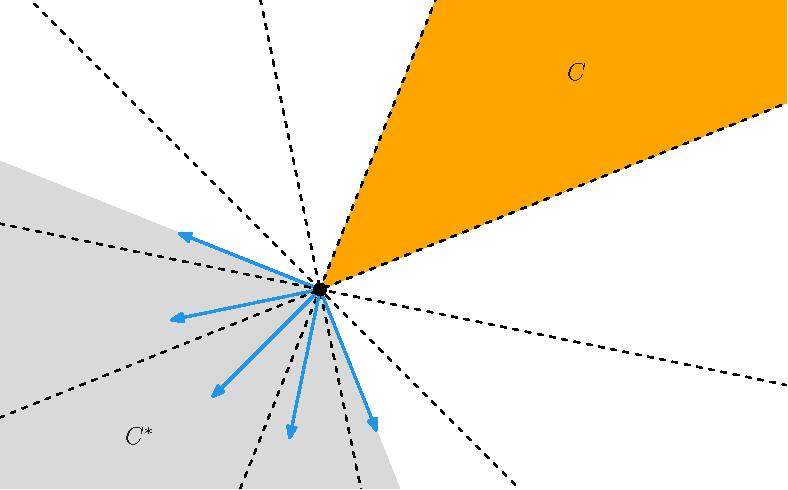
\includegraphics[width=0.7\textwidth]{fig/dual_cone.pdf}
\caption{A cone $K$ and its negative dual cone $-K^*$ (equivalently, its polar
  cone $K^\circ$), which can be easier to visualize. The set $-K^*$ is
  characterized by the normal vectors $y$ to all halfspaces $\{y : y^\T x \leq
  0\}$ containing $K$.}     
\label{fig:dual_cone}
\end{figure}

\section{Dual polyhedra*}
\label{sec:dual_polyhedra}

Recall (as covered in Chapter \ref{sec:polyhedra}), a polyhedron is an
intersection of halfspaces, $P = \{x : Ax \leq b\}$, for a matrix-vector pair 
$A,b$ of compatible dimensions. The \emph{dual polyhedron} to $P$ is defined as    
\index{polyhedron!dual polyhedron}
\index{polytope!dual polytope}
\begin{equation}
\label{eq:dual_polyhedron}
P^* = \{ y : y^\T x \leq 1, \; x \in P \}.
\end{equation}
The set $P^*$ is indeed a polyhedron (an intersection of halfspaces),  
% For example, Corollary 19.2.2 of Rockafellar (1970)
although this may be nonobvious at face value. The developments below will make
it clear that $P^*$ is polyhedral in the case that $P$ is bounded. The unbounded
case is discussed in Exercise \ref{ex:minkowski_weyl}. 
 
Let us assume henceforth that $P$ is bounded polyhedron, which recall we call a
polytope, with $0 \in \interior(P)$. While Theorem \ref{thm:hv_representation},
the main representation theorem for polytopes, can be established directly using 
algebraic arguments, we demonstrate in this section how it can be explained from 
the perspective of polyhedral duality. 

To this end, suppose that we have the H-representation $P = \{ x : Ax \leq
b\}$. Then by definition, 
\begin{align}
\nonumber
P^* &= \{ y : y^\T x \leq 1, \; \text{for all $x$ with $Ax \leq b$} \} \\
\label{eq:v_representation_dual}
&= \bigg\{ \sum_{i=1}^m t_i \frac{a_i}{b_i} : \text{$t_i \geq 0$, for
  $i=1,\dots,m$, and $\sum_{i=1}^m t_i = 1$} \bigg\}.
\end{align}
The second step above can be verified using Farkas' lemma (Exercise
\ref{ex:v_representation_dual}), where $a_1,\dots,a_m \in \R^d$ denote the rows
of $A$, and $b_1,\dots,b_m > 0$ (as $0 \in \interior(P)$). Defining $y_i =
a_i/b_i$, $i = 1,\dots,m$, we have thus produced the dual V-representation $P^*
= \conv\{y_1,\dots,y_m\}$.       

Suppose instead that we have the V-representation $P =
\conv\{x_1,\dots,x_n\}$. Again by definition,  
\begin{align}
\nonumber
P^* &= \big\{ y : y^\T x \leq 1, \; x \in \conv\{x_1,\dots,x_n\} \big\} \\
\label{eq:h_representation_dual}
&= \{ y : y^\T x_i \leq 1, \; i = 1,\dots,n \},
\end{align}
where the second step holds by convexity (Exercise
\ref{ex:h_representation_dual}). In other words, we have produced the dual
H-representation $P^* = \{ y : Xy \leq 1\}$, where $X$ is the matrix with rows
$x_1,\dots,x_n \in \R^d$.    

We have therefore established that the H-representation and V-representation for
polytopes are dual to one another: facets (halfspaces in an H-representation) of
$P$ correspond to vertices (points in a V-representation) of $P^*$, and vice 
versa. This dual relationship can actually be used as a key step in proving
Theorem \ref{thm:hv_representation} in the first place; see Exercise 
\ref{ex:hv_representation_dual}.    

There is in fact even more to be said about the relationship between $P$ and
$P^*$: not only vertices and facets, but all faces of $P$ and $P^*$ obey a
precise one-to-one correspondence. 

\begin{Theorem}
\label{thm:face_duality}
Let $P \subseteq \R^d$ be a polytope with $0 \in \interior(P)$, and let $P^*$ be
its dual polytope in \eqref{eq:dual_polyhedron}. Define a map $\Psi$ from faces
$\cF(P)$ of $P$ to faces $\cF(P^*)$ of $P^*$ by  
\[
\Psi(F) = \{ y \in P^* : y^\T x = 1, \; x \in F \}.
\]
Then $\Psi$ is a bijection. Furthermore, it is inclusion-reversing: $F \subseteq
G \implies \Psi(F) \supseteq \Psi(G)$, and it satisfies $\dim(F) + \dim(\Psi(F))
= d-1$ for all $F \in \cF(P)$. 
\end{Theorem}

This theorem, whose proof is outlined in Exercise \ref{ex:face_duality}, gives
us a rich way of understanding the relation between a polytope $P$ and its dual
$P^*$. Duality provides a representation map $\Psi$, which maps vertices of $P$
to facets of $P^*$, edges (1-faces) of $P$ to ridges ($(d-2)$-faces) of $P^*$,
and so on. In short, the  entire facial structure of $P$ is determined by $P^*$,
and vice versa. A canonical example of a dual polytope pair is given by the
$\ell_1$ and $\ell_\infty$ balls, explored in Exercise
\ref{ex:l1_linf_ball_duality}.    

\section{Polar sets*}
\label{sec:polar_sets}

Given a set $C$, its \emph{polar set} is defined by 
\index{polar set}
\begin{equation}
\label{eq:polar_set}
C^\circ = \{ y : y^\T x \leq 1, \; x \in C \}.
\end{equation}
For a polyhedron $P$, its polar set is simply another name for its dual
polyhedron \eqref{eq:dual_polyhedron}, $P^\circ = P^*$. Moreover, for a cone
$K$, its polar set is in fact the negative dual cone \eqref{eq:dual_cone},
$K^\circ = -K^*$: clearly we have $-K^* \subseteq K^\circ$, and for the opposite
inclusion, take any $y \in K^\circ$, $x \in K$, $t>0$, then observe that $y^\T x  
\leq 1 \implies y^\T (tx) \leq 1 \iff y^\T x \leq 1/t$, thus sending $t \to
\infty$ gives $y^\T x \leq 0$.          

One can check that the polar $C^\circ$ is always a closed convex set. When $C$
itself a closed convex set containing 0, the polar of its polar set is
\begin{equation}
\label{eq:polar_set_polar}
C^{\circ\circ} = C.
\end{equation}
As polarity generalizes duality for both polyhedra and cones, the above fact
implies $P^{**} = P$ for a polyhedron containing the origin, and also $K^{**} =
K$ for a closed convex cone, as claimed earlier in
\eqref{eq:dual_cone_dual}. The fact \eqref{eq:polar_set_polar} can be verified
using the separating hyperplane theorem (Exercise \ref{ex:polar_set_polar}). 

\begin{Example}
The \emph{tangent cone} to a set $C$ at a point $x \in C$ is defined as 
\index{normal cone!dual cone}
\index{tangent cone}
\begin{equation}
\label{eq:tangent_cone}
T_C(x) = \closure \Big\{ y : \text{there exists $\beta>0$ such that $x + \alpha
  y \in C$, for all $\alpha \in [0,\beta]$} \Big\}.  
\end{equation}
This is a closed cone, but need not be convex in general. However, if $C$ is
convex then $T_C(x)$ is convex too, and in this case it is actually the polar to
the normal cone, $(N_C(x))^\circ = T_C(x)$. Exercise \ref{ex:tangent_cone}
explores these and related details.     
\end{Example}

Polarity and conjugacy share a connection for characteristic functions. By
direct inspection, the conjugate of $I_C$, which recall (Example
\parref{xa:characteristic_function_conjugate}) is the support function $h_C =
I^*_C$, satisfies        
\[
h_C(y) \leq 1 \iff y \in C^\circ.
\]
Moreover, if $C$ is a cone, then we can see from the above that $h_C$ can
only take the values 0 and $\infty$ (since $h_C(y) \leq 1 \implies h_C(ty) = t
h_C(y) \leq 1$ for all $y \in C^\circ$ and $t>0$); more precisely, $h_C$ is 0 
on $C^\circ$ and $\infty$ otherwise, which leads to 
\begin{equation}
\label{eq:support_function_cone}
h_C = I_{C^\circ}.
\end{equation}
That is, the conjugate (support function) of the characteristic function of a
cone is the characteristic function of its polar cone. This fact will be useful
in derivations involving conic duality. 
  
\section{Conic duality*}
\label{sec:conic_duality}

We are now prepared to develop a theory of conic duality, which recall was
alluded to in Chapter \ref{sec:sdp_duality} (in particular, Corollary
\ref{cor:slater_sdp}). We will study an optimization problem said to be in
\emph{conic form}:     
% Note: convenient to write it this way because we are effectively separating
% out affine and nonaffine inequality constraints ahead of time ...
\begin{equation}
\label{eq:primal_conic}
\begin{alignedat}{2}
&\minimize_{x \in D} \quad && f(x) \\ 
&\st \quad && h(x) \leq_K 0 \\
& && Ax \leq b,
\end{alignedat}
\end{equation}
where $D \subseteq \R^d$ (viewed as the intersection of effective domains of
the functions in the optimization problem, which is typically implicit, but is
explicit here for convenience in what follows), $f : D \to \R$, $h : D \to 
\R^m$, $K \subseteq \R^m$ is a cone, $A \in \R^{k \times d}$, and $b \in
\R^k$. The relation $\leq_K$ in \eqref{eq:primal_conic} is defined by
\[
a \leq_K b \iff b-a \in K.
\]
When $K$ is a \emph{regular} cone $K$, which is a closed convex cone with
nonempty interior, that is \emph{pointed}: $K \cap -K = \{0\}$, one can check
that $\leq_K$ is indeed a partial ordering.\footnote{This means that it is
  reflexive: $a \leq_K a$, for all $a$; antisymmetric: $a \leq_K b$ and $b
  \leq_K a$ implies $a = b$; and transitive: $a \leq_K b$ and $b \leq_K c$
  implies $a \leq_K c$.}    
Notable examples are given by $K = \R_+^d$, the nonnegative orthant, where
$\leq_K$ reduces to the usual (coordinatewise) ordering $\leq$ on vectors, and
$K = \SS_+^d$, the positive semidefinite cone, where $\leq_K$ reduces to the
positive semidefinite ordering $\preceq$ on matrices.

\index{cone program}
As $h(x) \leq_K 0 \iff -h(x) \in K$, note that we can take $f$ to be linear and
$h$ to be affine in order to recover the cone program in \eqref{eq:cone_program}
from Chapter \ref{sec:cone_programs}. Thus, the general problem in conic form 
\eqref{eq:primal_conic} encompasses cone programs, and hence SDPs. Furthermore,
when we take $K = \R_+^d$, then problem \eqref{eq:primal_conic} is able to
recover standard convex programs, which were the focus of Chapter
\ref{chap:lagrangian_duality}. In this sense, the strong duality theorem below
both generalizes the previous one for standard convex programs (Theorem
\ref{thm:slater_condition}), and implies the previously claimed result for SDPs
(Corollary \ref{cor:slater_sdp}).

Defining \smash{$g(u,v) = \inf_{x \in D} \, \{ f(x) + u^\T h(x) + v^\T (Ax - b) 
  \}$}, the dual of \eqref{eq:primal_conic} is  
\begin{equation}
\label{eq:dual_conic}
\begin{alignedat}{2}
&\maximize_{u,v} \quad && g(u,v) \\ 
&\st \quad && u \geq_{K^*} 0 \\
& && v \geq 0,
\end{alignedat}
\end{equation}
which can be verified using familiar calculations in Lagrangian duality, along
with property \eqref{eq:support_function_cone} (Exercise
\ref{ex:dual_conic}). The following generalizes Slater's condition to problems
of conic form.  

\index{Slater's condition}
\index{strong duality}
\begin{Theorem}
\label{thm:slater_conic}
Consider the optimization problem \eqref{eq:primal_conic}. Assume the following.           

\begin{enumerate}[label=(\roman*)]
\item The set $D$ is convex, $K$ is a regular (closed, convex, pointed, with a
  nonempty interior) cone, $f : D \to \R$ is convex, and $h : D \to \R^m$ is
  $K$-convex, which means          
  \[
  h \big(t x + (1-t) y \big) \leq_K t h(x) + (1-t) h(y),  \quad \text{for all $x,y
  \in D$ and $t \in [0,1]$}.
  \]

\item There exists $x \in \relint(D)$, such that $Ax \leq b$ and $h(x) <_K 0
  \iff -h(x) \in \interior(K)$.
\end{enumerate}

Then strong duality holds: the optimal values $f^\star$ in
\eqref{eq:primal_conic} and $g^\star$ in the dual \eqref{eq:dual_conic} satisfy
$f^\star = g^\star$. Furthermore, when this common optimal value is finite, then
a dual solution exists (the optimal value in \eqref{eq:dual_conic} is attained).      
\end{Theorem}

This result is an extension and refinement of Slater's condition from Theorem 
\ref{thm:slater_condition}, and its proof proceeds similarly, outlined in
Exercises \ref{ex:convex_theorem_alternatives_conic} and \ref{ex:slater_conic}.  
Recall, applying Theorem \ref{thm:slater_conic} to SDPs yields Corollary 
\ref{cor:slater_sdp}, once we realize that we can learn from applying it to the
primal and the dual separately (the dual of the dual SDP being the primal SDP). 
A similar conclusion can be reached for cone programs (with $f,h$ being linear)
which we cover in Exercise \ref{ex:slater_cone_program}.

\section{Minimax theorems*}
\label{sec:minimax_theorems}

Now we broaden our perspective and study a real-valued function of a block
variable $(x,y) \in X \times Y$, denoted $L : X \times Y \to \R$. This can be
viewed as a generalization of the Lagrangian function featured in convex duality 
and the KKT conditions, with $x$ and $y$ representing the primal and dual
variables, constrained to lie in subsets $X \subseteq \R^d$ and $Y \subseteq  
\R^p$, respectively. We will investigate conditions under which $L$ admits a 
saddle point. What distinguishes our study here from that in previous chapters
is that the function $L$ is not restricted to be linear in $y$ (all Lagrangians
are linear in $u,v$).        

To be clear, as before, a point \smash{$(\bar{x}, \bar{y}) \in X \times Y$} is
said to be a saddle point of $L$ provided that  
\index{saddle point}
\begin{equation}
\label{eq:saddle_point2}
L(\bar{x}, y) \leq L(\bar{x}, \bar{y}) \leq L(x, \bar{y}) \quad \text{for any
  $x \in X$ and any $y \in Y$}. 
\end{equation}
An equivalent definition is 
\begin{equation}
\label{eq:saddle_point3}
\sup_{y \in Y} \, L(\bar{x}, y) \leq L(\bar{x}, \bar{y}) \leq \inf_{x \in X}
L(x, \bar{y}). 
\end{equation}
Defining the functions
\begin{equation}
\label{eq:saddle_functions}
f(x) = \sup_{y \in Y} \, L(x,y) \quad \text{and} \quad 
g(y) = \inf_{x \in X} \, L(x,y),
\end{equation}
we observe directly that $g(y) \leq L(x,y) \leq f(x)$, for any $x \in X$ and any 
$y \in Y$, whereas \eqref{eq:saddle_point3} calls for \smash{$(\bar{x},
  \bar{y})$} to satisfy \smash{$g(\bar{y}) \geq  L(\bar{x}, \bar{y}) \geq
  f(\bar{x})$}. This leads to the following conclusion (a generalization of
Theorem \ref{thm:saddle_point_optimality} for Lagrangian functions). 

\begin{Theorem}
\label{thm:saddle_point_optimality2}
For any function $L : X \times Y \to \R$, a point \smash{$(\bar{x}, \bar{y}) \in
  X \times Y$} is a saddle point as in \eqref{eq:saddle_point2} if and only if 
\smash{$\bar{x}$} minimizes $f$ over $X$, \smash{$\bar{y}$} maximizes $g$ 
over $Y$, and \smash{$f(\bar{x}) = g(\bar{y})$}, with $f$ and $g$ defined as in   
\eqref{eq:saddle_functions}. 
\end{Theorem}

When \smash{$(\bar{x}, \bar{y}) \in X \times Y$} is a saddle point, the
statement \smash{$f(\bar{x}) = g(\bar{y})$} is equivalent to 
\begin{equation}
\label{eq:saddle_point4}
\inf_{x \in X} \, \sup_{y \in Y} \, L(x,y) = \sup_{y \in Y} \, \inf_{x \in X} \,
L(x,y).
\end{equation}
The existence of a saddle point is therefore, according to
\eqref{eq:saddle_point4}, the assertion that ``minimax'' (min over $x$ and max
over $y$) and ``maximin'' problems (max over $y$ and min over $y$) are one in
the same. Conditions which guarantee the existence of saddle points are
thus often called \emph{minimax theorems}. 

We have already seen minimax theorems in Chapters \ref{sec:slater_condition},
\ref{sec:sdp_duality}, and \ref{sec:conic_duality}: these are (successively more  
general) versions of Slater's condition, which guarantees strong duality---and 
hence a saddle point of the associated Lagrangian $L$---in convex programs.   

The first and arguably the most famous minimax theorem is known as \emph{von
  Neumann's minimax theorem}, which concerns bilinear functions, of the form
$L(x,y) = x^\T P y$ (and assumes that $X,Y$ are probability simplices). Below is
a more general minimax result, known as \emph{Sion's minimax theorem}, for 
functions that are convex in their first argument and concave in their second.      

\index{Sion's minimax theorem}
\begin{Theorem}
\label{thm:sion_minimax}
Let $X \subseteq \R^d$ and $Y \subseteq \R^p$ be compact and let $L : X \times Y
\to \R$ be continuous. Assume that $L(\cdot,y)$ is convex for each fixed $y \in
Y$ and $L(x,\cdot)$ is concave for each fixed $x \in X$. Then there exists a
saddle point \smash{$(\bar{x}, \bar{y}) \in X \times Y$} of $L$, and thus
\eqref{eq:saddle_point4} holds. 
\end{Theorem}

Theorem \ref{thm:sion_minimax} is more general than (say) Theorem
\ref{thm:slater_condition} because $L$ is allowed to be concave (not
necessarily linear) in the argument $y$ representing the dual variable; at the
same time, it is also less general in that the sets $X,Y$ are assumed to be 
compact. Its proof is developed in Exercise \ref{ex:sion_minimax}.   

\section{Existence of minima, revisited*}
\label{sec:duality_minima}
\index{optimization problem!existence of solutions}

We once again revisit the existence of solutions in convex optimization
problems, now through the lens of duality. The refined form of Slater's
condition given in Theorem \ref{thm:slater_conic} (the conic formulation aside) 
showed that certain strict feasibility conditions on the primal problem imply
the existence of dual solutions (attainment of the dual optimal
value). Likewise, for a problem in which the dual of the dual is the primal, we
can apply Slater's condition to the dual problem in order to conclude the
existence of primal solutions (this was done for SDPs in Exercise
\ref{ex:lp_sdp_differences} parts a and b, and for cone programs in Exercise
\ref{ex:slater_cone_program}). 

Motivated to derive and extend the results in Theorem \ref{thm:existence_glms}
of Chapter \ref{sec:maximum_likelihood} on generalized linear models (GLMs), we
will study a problem of the form       
\begin{equation}
\label{eq:primal_legendre}
\minimize_\beta \quad f(X\beta) + h_C(\beta),
\end{equation}
where $f : \R^n \to (-\infty,\infty]$ is closed and convex, $X \in \R^{n \times
  d}$, and \smash{$h_C(\beta) = \sup_{z \in C} \, \beta^\T z$} is the support
function of a closed, convex, and nonempty set $C \subseteq \R^d$. The Fenchel
dual of \eqref{eq:primal_legendre} is
\begin{equation}
\label{eq:dual_legendre}
\maximize_u \quad -f^*(-u) \quad \st \quad X^\T u \in C,
\end{equation}
where we have used the fact that $h^*_C = I_C$ (by Example
\parref{xa:support_function_conjugate}). It is straightforward to check (again
using Fenchel duality, the fact that $f^{**} = f$ by
\eqref{eq:double_conjugate_identity}, and that $I^*_C = h_C$ by Example
\parref{xa:characteristic_function_conjugate}) that the dual of
\eqref{eq:dual_legendre} is \eqref{eq:primal_legendre}. Therefore, to reiterate
our strategy, we will investigate Slater's condition for
\eqref{eq:dual_legendre} in order to assert existence of solutions in
\eqref{eq:primal_legendre}.

To this end, let us assume that $f$ is of Legendre type (essentially smooth and
essentially strictly convex, as in Chapter \ref{sec:conjugate_smoothness}), as
this will enable us to easily relate the domain of its conjugate $f^*$ to $f$.
In particular, by Theorem \ref{thm:conjugate_legendre}, the gradient map $\nabla
f$ is a bijection from $\interior(\dom(f))$ to $\interior(\dom(f^*))$, which
means $\interior(\dom(f^*)) = \interior(\ran(\nabla f))$, where $\ran(\nabla f)$
denotes the range of $\nabla f$. Now, Slater's condition for
\eqref{eq:dual_legendre} requires the existence of $-u \in \interior(\ran(\nabla
f))$ and $X^\T u \in \relint(C)$, or
\begin{equation}
\label{eq:slater_dual_legendre}
\interior(\ran(\nabla f)) \cap (X^\T)^{-1} (\relint(-C)) \not= \emptyset,
\end{equation}
where $(X^\T)^{-1}$ denotes the inverse image under $X$. By Theorem
\ref{thm:slater_conic}, the condition \eqref{eq:slater_dual_legendre} guarantees
strong duality between \eqref{eq:primal_legendre}, \eqref{eq:dual_legendre}. To
ensure the existence of a primal solution, it remains to ensure that the optimal
dual value is finite, which happens if and only if the primal is feasible. This
leads us to the following result.

\begin{Theorem}
\label{thm:duality_minima}
Consider the optimization problem \eqref{eq:primal_legendre}, assumed to be
feasible, where $f$ is a closed and convex function of Legendre type, and $C$ is
a closed, convex, and nonempty set. Then, under condition
\eqref{eq:slater_dual_legendre}, a solution exists.
\end{Theorem}

To specialize to GLMs, where $X \in \R^{n \times d}$ is the feature matrix, we
take $f$ to be of the form  
\begin{equation}
\label{eq:glm_loss}
f(\eta) = -y^\T \eta + \Psi(\eta),
\end{equation}
where $y \in \R^n$ is the response vector, and $\Psi : \R^n \to (-\infty,
\infty]$ is the log-partition function, assumed to be itself of Legendre
type. Recall that for $f(X\beta)$ to represent the negative log likelihood in
linear regression, we take \smash{$\Psi(\eta) = \sum_{i=1}^n \eta_i^2/2$}; for
logistic regression, we take \smash{$\Psi(\eta) = \sum_{i=1}^n
  \log(1+e^{\eta_i})$}; and for Poisson regression, we take \smash{$\Psi(\eta) =
  \sum_{i=1}^n e^{\eta_i}$}. We thus see that \eqref{eq:primal_legendre} can 
represent regularized maximum likelihood in a GLM where the support function
$h_C$ acts as the regularizer. For example, if $C = \{ z : \|z\|_* \leq \lambda
\}$, then $h_C(\beta) = \lambda \|\beta\|$ is a norm penalty. Further, as
$\nabla f(\eta) = -y + \nabla \Psi(\eta)$, the condition
\eqref{eq:slater_dual_legendre} reduces to        
\begin{equation}
\label{eq:slater_dual_regularized_glm}
y \in \interior(\ran(\nabla \Psi)) + (X^\T)^{-1} (\relint(C)).
\end{equation}
We therefore arrive at the following conclusion for regularized GLMs. 

\index{generalized linear model!existence of solutions}
\begin{Corollary}
\label{cor:existence_regularized_glms}
Consider the regularized GLM problem \eqref{eq:primal_legendre}, assumed to be 
feasible, for $f$ as in \eqref{eq:glm_loss}, with $\Psi$ a closed and convex
function of Legendre type, and $C$ a closed, convex, and nonempty set. Then,
under condition \eqref{eq:slater_dual_regularized_glm}, a regularized GLM
solution exists.    

\setlength{\parindent}{\normalparindent}
Note in particular that when $C = \{0\}$, the condition in
\eqref{eq:slater_dual_glm} further reduces to  
\begin{equation}
\label{eq:slater_dual_glm}
y \in \interior(\ran(\nabla \Psi)) + \nul(X^\T),
\end{equation}
which guarantees the existence of an ordinary (unregularized) GLM solution.  
\end{Corollary}

For Poisson regression, recalling \smash{$\nabla_i \Psi(\eta) = e^{\eta_i}$}, $i
= 1,\dots,n$, we can see that $\interior(\ran(\nabla \Psi)) = \R_{++}^n$ is the 
positive orthant. In this case, it is clear that \eqref{eq:slater_dual_glm} is
equivalent to \eqref{eq:existence_poisson}, which verifies part (iii) of Theorem
\ref{thm:existence_glms}. For logistic regression, showing that
\eqref{eq:slater_dual_glm} is equivalent to \eqref{eq:existence_logistic} in
part (ii) of the same theorem requires a more nuanced argument, where a theorem
of the alternative (known as Stiemke's lemma) in needed to recast
\eqref{eq:slater_dual_glm}. This argument is outlined in Exercises
\ref{ex:stiemke_lemma}--\ref{ex:existence_logistic}. The case of a norm
penalty is studied in Exercise \ref{ex:existence_regularized_glms}. 

\SkipTocEntry\section*{Chapter notes}

This chapter has covered a wide range of topics related to duality, with the
title inspired by \cite{rockafellar1970convex} (Part III: Chapters 11--16). 
Fenchel duality is named after the developments in Fenchel's influential lecture
notes \cite{fenchel1951convex}, and was further developed by
\cite{rockafellar1963convex}. For more detail, we refer to
\cite{rockafellar1970convex} (Chapter 31). The geometry associated with convex 
duality---dual cones, dual polyhedra, and polar sets---is in it of itself a rich
topic. To learn more, we recommend \cite{rockafellar1970convex} (Chapters 14,
19), \cite{bertsekas2009convex} (Chapters 3.2, 3.3), \cite{grunbaum2003convex}  
(Chapters 3.1, 3.4), and \cite{ziegler1995lectures} (Chapters 2.3, 2.4).       

Our treatment of conic duality is based on \cite{bental2023convex} (Chapter
3.2), whose extension of Slater's condition for problems in conic form is
presented in our Theorem \ref{thm:slater_conic}. In addition, Exercises
\ref{ex:dubovitski_milutin_lemma}, \ref{ex:farkas_variations_conic}, 
\ref{ex:convex_theorem_alternatives_conic}, \ref{ex:slater_conic}, and   
\ref{ex:slater_cone_program} are all based the masterful treatment in
\cite{bental2023convex}.  

Sion's minimax theorem is named after \cite{sion1958general}, who extended  
von Neumann's minimax theorem \cite{vonneumann1928theorie} beyond bilinear   
functions. Also inspired by von Neumann, John Nash developed the concept of
(what is now called) \emph{Nash equilibria} \cite{nash1950equilibrium,
  nash1951noncooperative}, generalizing von Neumann's theorem in a different   
direction---to games in which the utility functions used by the two players  
(corresponding to $x$ and $y$ variables) are asymmetric, called non-zero-sum
games. Von Neumman's minimax theorem, Sion's minimax theorem, and the existence
of Nash equilibria can each be proved using fixed-point theorems, typically,
Kakutani's fixed-point theorem \cite{kakutani1941generalization} for set-valued
mappings. Instead, the proof laid out in Exercise \ref{ex:sion_minimax} below, 
which is based on \cite{bental2023convex} (Section 3.4), proceeds in such a way
that reveals connections to convex duality.    

The existence of solutions in optimization problems of regularized GLM-type
\eqref{eq:dual_legendre}, based on duality arguments, was studied in
\cite{ali2019generalized}. The arguments presented here are similar to those
from that paper. The fact that this approach is able to reproduce well-known 
results on the existence of logistic and Poisson regression solutions
is also from \cite{ali2019generalized}.    

\clearpage

\begin{xcb}{Exercises}
\begin{enumerate}[label=\thechapter.\arabic*]
\settowidth{\leftmargini}{00.00.\hskip\labelsep}
\item \label{ex:dual_norm_check}
  Prove that the dual norm \eqref{eq:dual_norm} is indeed a norm on $\R^d$ by
  verifying the following properties:  
  \begin{itemize}
  \item triangle inequality: $\|x+y\|_* \leq \|x\|_* + \|y\|_*$ for all $x,y \in 
  \R^d$;
  \item absolute homogeneity: $\|ax\|_* = |a|\|x\|_*$ for all $a \in \R$ and $x 
  \in \R^d$; and 
\item positive definiteness: $\|x\|_* \geq 0$ for all $x \in \R^d$, with
  equality if and only if $x=0$. 
  \end{itemize}

\item \label{ex:dual_norm_dual1}
  In this exercise, we investigate the dual of the dual of a norm $\|\cdot\|$: 
  \begin{equation}
  \label{eq:dual_norm_dual}
  \|x\|_{**} = \sup_{\|y\|_* \leq 1} \, x^\T y.
  \end{equation}
  Fixing any $x \in \R^d$, we will argue that $\|x\|_{**} = \|x\|$, in two
  steps.  

\begin{enumerate}[label=\alph*.]
\item Prove $\|x\|_{**} \leq \|x\|$ using H{\"o}lder's inequality
  \eqref{eq:holder_inequality}.  

\item Prove $\|x\|_{**} \geq \|x\|$ using the Hahn-Banach theorem. Hint:
  denoting $X = \R^d$, viewed as a vector space equipped with the norm
  $\|\cdot\|$, note that \eqref{eq:dual_norm_dual} can be rewritten as            
  \[
  \|x\|_{**} = \sup \{ F(x) : F \in X^*, \, \|F\|_{\op} \leq 1 \}.
  \]
  Here $X^*$ denotes the dual space of bounded linear functionals (real-valued 
  functions) on $X$, equipped with the norm \smash{$\|F\|_{\op} = \sup_{x \not 
    =  0} \, |F(x)| / \|x\|$.} Now define $L = \{ ax : a \in \R\}$, a
  1-dimensional subspace of $X$, and define $f : L \to \R$ by 
  $f(ax) = a\|x\|$. Show that $f$ is bounded and linear, with unit operator
  norm, hence by the Hahn-Banach theorem there exists a bounded linear
  functional $F$ on $X$ which agrees with $f$ on $L$, and itself has unit
  operator norm. Use this $F$ to show that $\|x\|_{**} \geq \|x\|$.  
\end{enumerate}

\index{norm!subgradients}
\index{dual norm!subgradients}
\item \label{ex:dual_norm_subgradients}
  In this exercise, we will prove Theorem \ref{thm:dual_norm_subgradients}. 

\begin{enumerate}[label=\alph*.] 
\item Prove that $\text{(i)} \iff \text{(iv)}$ using \eqref{eq:dual_norm}.
\item Prove that $\text{(i)} \iff \text{(v)}$ using \eqref{eq:norm_dual2}.
\item Prove that $\text{(ii)} \iff \text{(iv)}$ using
  \eqref{eq:norm_subgradients}, which comes from applying the Danskin-Bertsekas
  theorem \eqref{eq:danskin_bertsekas} to \eqref{eq:dual_norm}.
\item Prove that $\text{(iii)} \iff \text{(v)}$ using
  \begin{equation}
  \label{eq:dual_norm_subgradients}
  \partial \|y\|_* = \{ x : \|x\| \leq 1, \, x^\T y = \|y\|_* \},
  \end{equation}
  which comes from applying the Danskin-Bertsekas theorem
  \eqref{eq:danskin_bertsekas} to \eqref{eq:norm_dual2}. 
\end{enumerate}

\index{lp norm@$\ell_p$ norm!dual norm}
\item \label{ex:lp_norm_dual}
  In this exercise, we prove $(\|\cdot\|_p)_* = \|\cdot\|_q$, as stated in
  Example \parref{xa:lp_norm_dual}, for $p,q \geq 1$ such that $1/p + 1/q = 1$. 
  It suffices to prove $x^\T y \leq \|x\|_p \|y\|_q$ for all $x,y$ (traditional
  H{\"o}lder's inequality, for $\ell_p$ norms), where equality can always be
  obtained for each $x$ (at some $y$). We consider the cases $p = 1$ and $p > 
  1$ separately.            

\begin{enumerate}[label=\alph*.] 
\item Argue directly that $x^\T y \leq \|x\|_1 \|y\|_\infty$, with equality if
  $y_i = \sign(x_i)$, $i = 1,\dots,d$.

\item When $p > 1$, argue first that we can take $\|x\|_p= \|y\|_q = 1$,  
  without any loss of generality. Then argue that $x_i y_i \leq |x_i|^p / p +
  |y_i|^q / q$, using Young's inequality, and sum this up over each $i =
  1,\dots,d$ to arrive at $x^\T y \leq \|x\|_p \|y\|_q$, with equality if
  $|x_i|^p = c |y_i|^q$ for $c > 0$. 
\end{enumerate}

\item \label{ex:scaled_euclidean_norm_dual}
  Consider the optimization problem
  \[
  \maximize \quad y^\T x \quad \st \quad x^\T A x \leq 1. 
  \]
  Prove that the supremum is attained at \smash{$x = A^{-1} y / \sqrt{y^\T
    A^{-1} y}$}, and so \smash{$(\|y\|_A)_* = \sqrt{y^\T A^{-1} y}$}, as stated
  in Exercise \parref{xa:scaled_euclidean_norm_dual}. 

\index{trace norm!dual norm}
\item \label{ex:trace_norm_dual}
  To prove $(\|\cdot\|_{\tr})_* = \|\cdot\|_{\op}$, as stated in Exercise
  \parref{xa:trace_norm_dual}, we will verify that $(\|\cdot\|_{\op})_* = 
  \|\cdot\|_{\tr}$, where to be clear,
  \[
  (\|X\|_{\op})_* = \sup_{\|Z\|_{\tr} \leq 1} \, \langle Z, X \rangle, 
  \]
  and $\langle Z, X \rangle = \tr(Z^\T X)$. We proceed in two steps; in what
  follows, let $X = U \Sigma V^\T$ be the SVD of $X \in \R^{k \times d}$.

\begin{enumerate}[label=\alph*.] 
\item Prove $(\|X\|_{\op})_* \leq \|X\|_{\tr}$ by direct calculation. Hint:
  given any $Z$ such that $\|Z\|_{\op} \leq 1$, argue that 
  \[
  \langle Z, X \rangle = \langle U^\T Z V, \Sigma \rangle = \sum_{i=1}^d u_i^\T
  Z v_i \sigma_{ii}, 
  \]
  where $u_i,v_i$ denote the $i\th$ columns of $U,V$, respectively, for $i =
  1,\dots,d$. Then argue that each $u_i^\T Z v_i \leq 1$, as $u_i,v_i$ have 
  unit $\ell_2$ norm and $\|Z\|_{\op} \leq 1$.

\item Prove $(\|X\|_{\op})_* \geq \|X\|_{\tr}$ by studying $\langle Z, X
  \rangle$ with $Z = U V^\T$. Hint: verify that now  
  \[
  \langle Z, X \rangle = \langle U^\T Z V, \Sigma \rangle = \sum_{i=1}^d
  \sigma_{ii}.
  \]
\end{enumerate}

% Recall that the Schatten $p$-norm on matrices is defined, for $p \geq 1$, by    
% \[
% \|X\|_p =  \|\sigma(X)\|_p,
% \]
% with the right-hand representing the usual $\ell_p$ norm of the vector
% $\sigma(X) = (\sigma_1(X), \dots, \sigma_n(X))$ of singular values of a matrix 
% $X \in \R^{n \times d}$. Consider
% \[
% (\|X\|_p)_* = \sup_{\|Z\|_p \leq 1} \, \langle Z, X \rangle,
% \]
% where $\langle Z, X \rangle = \tr(Z^\T X)$. Prove that $(\|X\|_p)_* =
% \|X\|_q$, where $1/p + 1/q = 1$.   

\item \label{ex:norm_squared_conjugate}
  We will derive some properties associated with the pair of set-valued
  operators   
  \begin{align*}
  d(x) &= \|x\| \cdot \partial \|x\|, \\
  d^*(y) &= \|y\|_* \cdot \partial \|y\|_*.
  \end{align*}

\begin{enumerate}[label=\alph*.] 
\item Prove that $\|x\| = \|y\|_*$, for $y \in d(x)$.
\item Prove that $x^\T y = \|x\|^2$, for $y \in d(x)$. 
\item For $f(x) = \frac{1}{2} \|x\|^2$, prove that $\partial f(x) = d(x)$. 
\item For $f^*(y) = \sup_x \, \{ y^\T x - f(x) \}$, prove that the supremum
  defining $f^*(y)$ is achieved for $y \in d(x)$. Plug this in, and use parts a
  and b, to verify \eqref{eq:norm_squared_conjugate}. 
\item Prove that $d(x) = \argmax_y \, \{ x^\T y - \frac{1}{2} \|y\|_*^2 \}$, and 
  $d^*(y) = \argmax_x \, \{ y^\T x - \frac{1}{2} \|x\|^2 \}$. 
\item Prove that $y \in d(x) \iff x \in d^*(y)$.
\end{enumerate}

\item \label{ex:dual_norm_dual2}
  Consider the optimization problem 
  \[
  \minimize_z \quad \|z\| \quad \st \quad z = x,
  \]
  whose optimal criterion value is $f^\star = \|x\|$. Show that its Lagrange 
  dual problem is 
  \[
  \maximize_u \quad u^\T x \quad \st \quad \|u\|_* \leq 1,
  \]
  whose optimal criterion value is $g^\star = \|x\|_{**}$. Argue that strong 
  duality holds, $f^\star = g^\star$, which translates to $\|x\|_{**} = \|x\|$. 

\item \label{ex:dual_norm_dual3}
  Use \eqref{eq:norm_squared_conjugate}, and the fact that $f^{**} = f$ for
  closed convex $f$, as in \eqref{eq:double_conjugate_identity}, to verify
  $\|x\|_{**} = \|x\|$.  

\index{lasso!dual problem}
\item \label{ex:lasso_fenchel_dual}
  For \smash{$f(z) = \frac{1}{2} \|y-z\|_2^2$}, prove either by direct
  calculation or calculus rules for conjugacy that \smash{$f^*(u) = \frac{1}{2}
    \|y+u\|_2^2 - \frac{1}{2} \|y\|_2^2$}. Use this to show that Fenchel
  duality, as given in Example \parref{xa:fenchel_norm}, reproduces the lasso 
  dual in \eqref{eq:lasso_dual}.

\index{support vector machine!hinge form}
\index{support vector machine!dual problem}
\item \label{ex:svm_fenchel_dual}
  Consider the SVM in hinge form, for labels $y_i \in \{ -1, 1\}$ and features
  $x_i \in \R^d$, $i=1,\dots,n$,     
  \begin{equation}
  \label{eq:svm_hinge2}
  \minimize_{\beta_0,\beta} \quad C \sum_{i=1}^n \big[1 - y_i(\beta_0 + x_i^\T 
  \beta)\big]_+ + \frac{1}{2} \|\beta\|_2^2.
  \end{equation}
  We simplify our study, in preparation for examining Fenchel duality, by
  omitting the intercept term $\beta_0$. Denote by $y \in \R^n$ the label
  vector, $X \in \R^{n \times d}$ the feature matrix (with $i\th$ row $x_i^\T$),
  and \smash{$\tilde{X} = \diag(y) X$}. Then the above problem (without
  intercept) can be recast as      
  \begin{equation}
  \label{eq:svm_hinge3}
  \minimize_\beta \quad f(\tilde{X} \beta) + \frac{1}{2} \|\beta\|_2^2, 
  \end{equation}
  where $f(z) = C \sum_{i=1}^n (1-z_i)_+$. To reproduce the dual
  \eqref{eq:svm_dual}, we proceed in steps. 

\begin{enumerate}[label=\alph*.] 
\item Prove by direct calculation that $f^*(u) = \one^\T u \cdot
  I_{[-C,0]^n}(u)$.   

\item Use Fenchel duality, as given in Example \parref{xa:fenchel_norm_squared}, 
  to prove that the dual of \eqref{eq:svm_hinge3} is
  \begin{alignat*}{2}
  &\maximize_u \quad && \one^\T u - \frac{1}{2} \|\tilde{X}^\T u\|_2^2 \\ 
  &\st \quad && u \in [0,C]^n.
  \end{alignat*}

\item Adapt the arguments in the previous parts to accommodate the intercept in
  the original problem \eqref{eq:svm_hinge2}, and show that the resulting
  Frenchel dual reproduces \eqref{eq:svm_dual}. Hint: the presence of intercept
  will require you to compute the conjugate of \smash{$(\beta_0, \beta) \mapsto 
    \frac{1}{2} \|\beta\|_2^2$}.    
\end{enumerate}

\item When is the dual of dual problem the primal problem? Describe a class of
  problems in which this holds, using Fenchel duality.   

\index{Dubovitski-Milutin lemma}
\item \label{ex:dubovitski_milutin_lemma} 
  Let $K_1,\dots,K_m$ be cones, and $K = K_1 \cap \dots \cap K_m$. 

\begin{enumerate}[label=\alph*.] 
\item Prove that $K^* \supseteq \closure(K_1^* + \cdots + K_m^*)$. 
\item Assuming additionally that $K_1,\dots,K_m$ are closed, prove that
  $K^* = \closure(K_1^* + \cdots + K_m^*)$. Hint: use the strict separating
  hyperplane theorem, from Exercise \ref{ex:farkas_lemma}.      
  % Proposition 1.2.6 in Ben-Tal and Nemirovski (2023) 

\item Assuming additionally that $K_1,\dots,K_m$ are convex (altogether, these
  are closed convex cones), and $K_1 \cap \interior(K_2) \cap \cdots \cap
  \interior(K_m) \not= \emptyset$, prove that $K_1 ^* + \cdots + K_m^*$ is
  closed, thus 
  \[
  K^* = K_1^* + \cdots + K_m^*.
  \] 
  This is known as the \emph{Dubovitski-Milutin lemma}. Hint: consider a
  sequence $y_j = \sum_{i=1}^k y_{ij}$, with $y_{ij} \in K_i^*$ for $j =
  1,2,3,\dots$ and each $i$, where $y_j \to y$ as $j \to \infty$. It remains to
  show that $y \in K_1^* + \cdots + K_m^*$. For this, use the existence of $x
  \in K_1 \cap \interior(K_2) \cap \cdots \cap \interior(K_m)$ to show that
  $y_{ij}$, $j = 1,2,3,\dots$ is a bounded sequence for each $i$, and therefore,
  passing to a subsequence if needed, it has a subsequence converging to a point
  in $K_i^*$.  
  % Proposition 1.2.7 in Ben-Tal and Nemirovski (2023) 
\end{enumerate}

\index{Farkas' lemma}
\item \label{ex:farkas_variations_conic} 
  In this exercise, we will show that the Dubovitski-Milutin lemma, studied in
  the last exercise, leads to an important variation on Farkas' lemma. This
  result will generalize the result from Exercise \ref{ex:farkas_variations}
  part b, which was a key tool used in proving the convex theorem of
  alternatives from Exercise \ref{ex:convex_theorem_alternatives}. Given $A \in
  \R^{k \times d}$, $b \in \R^k$, $g \in \R^d$, $h \in \R$, and a convex set $D
  \subseteq \R^d$, with $b \geq 0$ and $0 \in \interior(D)$, consider two
  statements:        
  \begin{itemize}
  \item for all $x \in D$, it holds that $Ax \leq b \implies g^\T x \leq h$;  
  \item there exists $\mu \in \R^k$ such that $\mu \geq 0$ and $\mu^\T (Ax - b) 
    \geq g^\T x - h$ for all $x \in D$.
  \end{itemize}
  We will prove that these two statements are equivalent in what follows.
  % Following Lemma 3.2.1 in Ben-Tal and Nemirovski (2023)
  
\begin{enumerate}[label=\alph*.]
\item Prove that the second statement implies the first.

\item To prove that the first statement implies the second, start by defining 
  \[
  K_1 = \closure \Big\{ (x,t) \in \R^d \times \R: t > 0, \, x/t \in D \Big\}
  \quad \text{and} \quad K_2 = \Big\{ (x,t) \in \R^d \times \R: Ax \leq tb
  \Big\}.  
  \]
  Show that these are closed convex cones, with $\interior(K_1) \cap K_2 \not= 
  \emptyset$. 

\item Define $f = (g,-h) \in \R^{d+1}$, and show that $f^\T (x,t) \leq 0$ for
  all $(x,t) \in K_1 \cap K_2$.  

\item Use Exercise \ref{ex:dubovitski_milutin_lemma} part c to argue that we can
  write $f = \psi + \phi$, where $\psi^\T(x,t) \leq 0$ for all $x \in K_1$, and
  $\phi^\T (x,t) \leq 0$ for all $x \in K_2$. 

\item Use Exercise \ref{ex:farkas_variations} part a to argue that there exists
  $\mu \geq 0$ with $[A \, -b]^\T \mu = \phi$, in other words, $\phi^\T (x,t) =
  \mu^\T (Ax - tb)$ for all $x,t$. Use this to prove the desired result.        
\end{enumerate}
  
\item \label{ex:v_representation_dual}
  To verify \eqref{eq:v_representation_dual}, argue that the inclusion
  $\supseteq$ follows directly, whereas the inclusion $\subseteq$ follows using
  the Farkas' lemma variation from Exercise \ref{ex:farkas_variations} part b
  (or Exercise \ref{ex:farkas_variations_conic} with $D = \R^d$). Hint: fixing
  $y$ such that $Ax \leq b$ implies $y^\T x \leq 1$; we know that there exists  
  $\mu \geq 0$ such that $\mu^\T (Ax - b) \geq y^\T x - 1$ for all $x \in 
  \R^d$. Show that this implies $y = A^\T \mu$, and $\mu^\T b \leq 1$.
  We can then reparametrize, using $b_1,\dots,b_m > 0$, since $0 \in
  \interior(P)$, to obtain the desired statement. 

\item \label{ex:h_representation_dual}
  To verify \eqref{eq:h_representation_dual}, argue that the inclusion
  $\subseteq$ follows directly, whereas the inclusion $\supseteq$ follows
  by convexity of the set $\{x : y^\T x \leq 1\}$ for a given $y$.

\item \label{ex:hv_representation_dual}
  In this exercise, we step through a proof of the main representation theorem,
  Theorem \ref{thm:hv_representation}, for polytopes. We treat each direction 
  separately. 

\begin{enumerate}[label=\alph*.]
\item Suppose $P = \{x : Ax \leq b\}$ is an H-representation and $P$ is
  bounded. Use the fact that $P$ has a finite number of faces (Exercise
  \ref{ex:face_structure} part f), along with the Krein-Milman theorem
  (Exercise \ref{ex:extreme_points} part b), to show that $P =
  \conv\{x_1,\dots,x_n\}$ for vertices $x_1,\dots,x_n$.

\item Suppose $P = \conv\{x_1,\dots,x_n\}$ is a V-representation. Show that the
  dual polytope $P^*$ has an H-representation, then use the argument from part a
  applied to $P^*$, and duality once again along with $P^{**} = P$ by
  \eqref{eq:polar_set_polar}, to form an H-representation for $P$.    
\end{enumerate}

\item \label{ex:face_duality}
  This exercise outlines the proof of Theorem \ref{thm:face_duality}. It is
  trivial to check that $\Psi(\emptyset) = P^*$ and $\Psi(P) = \emptyset$, and
  we restrict our attention to a proper face $F \in \cF(P)$.  
% Following Theorem 4 in Chapter 3.4 of Grunbaum (2003)

\begin{enumerate}[label=\alph*.]
\item Let $x_0 \in \relint(F)$, and $F^* = \{ y \in P^* : y^\T x_0 = 1 \}$.
  Prove that $\Psi(F) = F^*$, and so $\Psi(F)$ is indeed a face of
  $P^*$. Hint: suppose that $\Psi(F) \not= F^*$, and take $y_0 \in F^* \setminus
  \Psi(F)$. Argue there exists $x_1 \in F$ such that $y_0^\T x_1 < 1$. Use $x_0
  \in \relint(F)$ to argue that $y_0^\T x_0 < 1$. 

\item Prove the inclusion-reversing property: given $G \supseteq F$, we have
  $\Psi(G) \subseteq \Psi(G)$.  

\item Prove the dimensionality property: $\dim(F) + \dim(\Psi(F)) = d-1$.  
\end{enumerate}

\item \label{ex:l1_linf_ball_duality}
  Consider the $\ell_1$ and $\ell_\infty$ balls in $\R^d$,
  \[
  P = \bigg\{ x : \sum_{i=1}^d |x_i| \leq 1 \bigg\} \quad \text{and} \quad 
  Q = \bigg\{ x : \max_{i=1,\dots,d} \, |x_i| \leq 1 \bigg\}. 
  \]
  In geometry these are often referred to as the \emph{cross-polytope} and
  \emph{hypercube}, respectively.  

\begin{enumerate}[label=\alph*.]
\item Prove directly with a counting argument that the number of $k$-faces of
  $P$ is $2^{k+1} {d \choose k+1}$.  

\item Prove directly with a counting argument that the number of $k$-faces of
  $Q$ is $2^{d-k} {d \choose d-k}$. 

\item Prove that $P^* = Q$, and check that the relationship between the faces of
  $P$ and $Q$ from Theorem \ref{thm:face_duality} is consistent with parts a and
  b above. 
\end{enumerate}

\item \label{ex:minkowski_weyl}
  We say that a set $C \subseteq \R^d$ is \emph{finitely generated} provided
  there exists $x_1,\dots,x_n \in \R^d$ and $k \leq n$ such that $C = 
  \conv\{x_1,\dots,x_k\} + \cone\{x_{k+1},\dots,x_n\}$, or in other words  
  \[
  C = \bigg\{
  \sum_{i=1}^n t_i x_i : \text{$t_i \geq 0$, for $i=1,\dots,n$, and
    $\sum_{i=1}^k t_i = 1$} \bigg\}.  
  \]
  When $k = n$, note that $C$ reduces to the convex hull of $x_1,\dots,x_n$,
  which is bounded, but when $k < n$, the set $C$ will be unbounded. A 
  generalization of Theorem \ref{thm:hv_representation}, sometimes referred to
  as the \emph{Minkowski-Weyl theorem}, is as follows: 
  \index{Minkowski-Weyl theorem}
  \index{polyhedron!dual polyhedron}
  \begin{equation}
  \label{eq:hv_representation_generalized}
  \text{a set $P$ is a polyhedron if and only if it is finitely generated.}
  \end{equation}
  % For example, Theorem 19.1 in Rockafellar (1970)
  In what follows, we will use this generalization to prove certain facts about
  polyhedra. Denote by $P = \{x : Ax \leq b\} \subseteq \R^d$ a polyhedron, and
  $f : \R^d \to \R^m$ a linear transformation.     

\begin{enumerate}[label=\alph*.]
\item Show that the preimage $f^{-1}(P)$ of $P$ under $F$ is a polyhedron. 

\item Show that the image $f(P)$ of $P$ under $F$ is a polyhedron. Hint: use
  \eqref{eq:hv_representation_generalized}. 

\item Show that the dual $P^*$ defined in \eqref{eq:dual_polyhedron} is a 
  polyhedron. Hint: use \eqref{eq:hv_representation_generalized}.
\end{enumerate}

\item \label{ex:polar_set_polar}
  Given an arbitrary set $C$, consider the polar of its polar set:
  \[
  C^{\circ\circ} = \{ x : x^\T y \leq 1, \; y \in C^\circ \}.
  \]
  In this exercise, we verify \eqref{eq:polar_set_polar}, assuming $C$ is closed
  and convex with $0 \in C$.
  
\begin{enumerate}[label=\alph*.] 
\item Prove that $C \subseteq C^{\circ\circ}$.
\item Prove that $C \supseteq C^{\circ\circ}$. Hint: fix $x_0 \notin C$, and
  argue that $x_0 \notin C^{\circ\circ}$ using the strict version of the
  separating hyperplane theorem given in Exercise \ref{ex:farkas_lemma}. Use $0
  \in C$ to show that the separating hyperplane can be expressed as $y^\T x_0 >
  1$ and $y^\T x < 1$ for all $x \in C$.
\end{enumerate}

\index{normal cone!dual cone}
\index{tangent cone}
\item \label{ex:tangent_cone}
  This exercise studies the tangent cone \eqref{eq:tangent_cone} to a set $C$ at
  a point $x \in C$. 
% See Theorems 6.5 and 6.9 of Rockafellar and Wets (2009), although our
% presentation is slightly different, but equivalent for convex sets 

\begin{enumerate}[label=\alph*.] 
\item Give an example to show that $T_C(x)$ can be nonconvex.
\item For convex $C$, prove that $T_C(x)$ is convex. 
\item For convex $C$, prove that $N_C(x) = (T_C(x))^\circ$ and thus
  $(N_C(x))^\circ = T_C(x)$. Hint: for the first claim, establish each inclusion
  ($\subseteq$ and $\supseteq$) separately. Only one requires convexity.        
\end{enumerate}

\item \label{ex:convex_theorem_alternatives_conic}
  Given a set $D$, cone $K$, functions $f,h$, and matrix-vector pair $A,b$,
  consider the problems:
  \begin{align}
  \label{eq:feasibility_conic1}
  &\begin{alignedat}{2}  
  &\find \quad && x \\  
  &\st \quad && f(x) < c \\
  & && h(x) \leq_K 0 \\
  & && Ax \leq b \\
  & && x \in D,
  \end{alignedat} \\[10pt]
  \label{eq:feasibility_conic2}
  &\begin{alignedat}{2}  
  &\find \quad && u,v \\ 
  &\st \quad && \inf_{x \in D} \, \big\{ f(x) + u^\T h(x) + v^\T (Ax - b) \big\}
  \geq c \\  
  & && u \geq_{K^*} 0 \\ 
  & && v \geq 0.
  \end{alignedat}
  \end{align}
  The value of $c$ here is fixed and arbitrary. Following Theorem
  3.2.2 in \cite{bental2023convex}, we will prove what these authors call the
  \emph{convex theorem of alternatives} for problems in conic form, which
  generalizes the result in Exercise \ref{ex:convex_theorem_alternatives}. This
  theorem says that under conditions (i) and (ii) in Theorem
  \ref{thm:slater_conic}, problem \eqref{eq:feasibility_conic2} is feasible if 
  and only if \eqref{eq:feasibility_conic1} is infeasible.    
  
\begin{enumerate}[label=\alph*.]
\item Assume that problem \eqref{eq:feasibility_conic2} is feasible. Prove that
  problem \eqref{eq:feasibility_conic1} is infeasible. Hint: argue the
  contrapositive, recalling that $K^*$ is the dual cone, and \smash{$u
    \geq_{K^*} 0 \iff u \in K^*$}. Note that this part of the argument does not
  use conic Slater's condition.   
  
\item The other direction---that infeasibility of \eqref{eq:feasibility_conic2}
  implies feasibility of \eqref{eq:feasibility_conic1}---is much more involved,
  and we will prove this in several steps, following closely the structure of
  arguments in Exercise \ref{ex:convex_theorem_alternatives}. We assume without
  a loss of generality that $c = 0$, and that $x = 0$ satisfies condition (ii)
  in Theorem \ref{thm:slater_conic}. Define the sets         
  \begin{align*}
  S &= \Big\{ (t_0, t_1) \in \R \times \R^m : t_0 < 0, \, t_1 \leq_K 0 \Big\},
    \\    
  T &= \Big\{ (t_0, t_1) \in \R \times \R^m : \text{there exists $x \in D$ such
      that $f(x) \leq t_0$, $h(x) \leq_K t_1$, and $Ax \leq b$} \Big\}.  
  \end{align*}
  Assume that \eqref{eq:feasibility_conic1} is infeasible. Prove that there
  exists a nonzero vector $a = (a_0, a_1) \in \R \times \R^m$, with $a_0 \geq 0$
  and \smash{$a_1 \geq_{K^*} 0$}, such that    
  \[
  \inf_{t \in T} \, a^\T t \geq 0.  
  \]
  Hint: apply the separating hyperplane theorem, Theorem
  \ref{thm:separating_hyperplane}, to $S,T$. Then argue that we must have $a_0
  \geq 0$, \smash{$a_1 \geq_{K^*} 0$}, and $b = 0$ in the supporting hyperplane.    

\item Prove that $a_0 > 0$. Hint: assume in order to achieve a contradiction 
  that $a_0 = 0$. Then use $(f(0), h(0)) \in T$, and the fact that $x = 0$
  satisfies condition (ii) in Theorem \ref{thm:slater_conic}, by assumption,
  to conclude $a_1 = 0$.

\item Define $\alpha = a_1 / a_0 \in \R^m$, and  
  \[
  F(x) = f(x) + \alpha^\T h(x),
  \]
  where $h(x) = (h_1(x), \dots, h_m(x))$. Noting that \smash{$\alpha \geq_{K^*}
    0$} (as $a_0 > 0$ and \smash{$a_1 \geq_{K^*} 0$}), prove 
  \[
 \text{for all $x \in D$}, \quad Ax \leq b \implies F(x) \geq 0.
  \]
  Hint: for any $x \in D$ with $Ax \leq b$, we have $t = (f(x), h(x)) \in T$, so
  that $a^\T t \geq 0$.

\item In what remains, we seek to show that there exists $\beta \in \R^k$ such
  that $\beta \geq 0$ and  
  \begin{equation}
  \label{eq:feasibility_conic3}
  F(x) + \beta^\T (Ax - b) \geq 0, \quad \text{for all $x \in D$}. 
  \end{equation}
  Notice that this would complete the proof as it would prove that 
  \eqref{eq:feasibility_conic2} is feasible, for $u = \alpha$ and $v = \beta$
  (recall that we have taken $c = 0$). Towards verifying the existence of such a
  vector $\beta$, define the sets     
  \begin{align*}
  G &= \Big\{ (x, z) \in \R^d \times \R : x \in D, \, Ax \leq b, \, z < 0
      \Big\}, \\    
  H &= \Big\{ (x, z) \in \R^d \times \R : x \in D, \, F(x) \leq z \Big\},  
  \end{align*}
  Prove that there exists a nonzero vector $(w, \eta) \in \R^d \times \R$ such
  that  
  \[
  \sup \, \Big\{ w^\T x + \eta z : x \in D, \, Ax \leq b, \, z < 0 \Big\} \leq 
  \inf \, \Big\{ w^\T x + \eta z : x \in D, \, F(x) \leq z \Big\}. 
  \]
  Hint: apply the separating hyperplane theorem again, this time to $G,H$. 

\item Argue that $\eta \geq 0$, so that 
  \[
  \sup \Big\{ w^\T x : x \in D, \, Ax \leq b \Big\} \leq \inf \Big\{ w^\T x +
  \eta F(x) : x \in D \Big\}.
  \]

\item Argue further that $\eta > 0$, so that by defining $\rho = w / z$, we
  have  
  \[
  \sup \Big\{ \rho^\T x : x \in D, \, Ax \leq b \Big\} \leq \inf \Big\{
  \rho^\T x + F(x) : x \in D \Big\}.
  \]
  Hint: assume for the sake of contradiction that $\eta = 0$. Then as the origin
  $x = 0$ satisfies condition (ii) from Theorem \ref{thm:slater_conic}, the
  left-hand side in the display from part f is at least zero, so that $w^\T x
  \geq 0$ for all $x \in D$, which can only happen (recalling $0 \in
  \interior(D)$, and assuming without a loss of generality that $D$ is
  full-dimensional) if $w = 0$.

\item Let $\theta = \sup \, \{\rho^\T x : x \in D, \, Ax \leq b\}$. Then $x \in
  D$ and $Ax \leq b \implies \rho^\T x \leq \theta$, hence by Exercise 
  \ref{ex:farkas_variations_conic}, there exists a vector $\beta \geq 0$ such that
  $\beta^\T (Ax - b) \geq \rho^\T x - \theta$ for all $x \in D$. Use this along 
  with part g to establish \eqref{eq:feasibility_conic3} and complete the proof.    
\end{enumerate}

\index{Slater's condition}
\item \label{ex:slater_conic}
  In this exercise, we prove the conic generalization of Slater's condition for
  strong duality, in Theorem \ref{thm:slater_conic}. Let $f^\star, g^\star$ be
  the optimal values in \eqref{eq:primal_conic} and \eqref{eq:dual_conic},
  respectively. Note that if $f^\star = -\infty$, then the desired conclusion
  $f^\star = g^\star$ is already implied by weak duality. Hence, assume that
  $f^\star > -\infty$, and use the result in Exercise
  \ref{ex:convex_theorem_alternatives_conic} to prove $f^\star = g^\star$, and
  there exists dual feasible $u,v$ which achieve the optimal criterion
  value. Hint: set $c = f^\star$.      

\item \label{ex:dual_conic}
  We derive the dual of problem \eqref{eq:primal_conic}. Show that we can
  rewrite this as  
  \begin{alignat*}{2}
  &\minimize_{x,z} \quad && f(x) + I_K(z) \\ 
  &\st \quad && h(x) = -z \\ 
  & && Ax \leq b,
  \end{alignat*} 
  whose Lagrangian is
  \[
  L(x,z,u,v) = f(x) + I_K(z) + u^\T (h(x) + z) + v^\T (Ax - b).
  \]
  Then, by minimizing over $x,z$, and using $I^*_K = I_{K^\circ} = I_{-K^*}$
  from \eqref{eq:support_function_cone}, show that the dual problem is as
  claimed in \eqref{eq:dual_conic}.  

\index{cone program!dual problem}
\item \label{ex:slater_cone_program}
  Recall that a cone program is a special case of \eqref{eq:primal_conic} where 
  $f(x) = c^\T x$ and $h(x) = Px - q$, for $c \in \R^d$, $P \in \R^{m \times d}$,
  and $q \in \R^m$, explicitly   
  \begin{equation}
  \label{eq:primal_cone_program}
  \begin{alignedat}{2}
  &\minimize_x \quad && c^\T x \\ 
  &\st \quad && Px \leq_K q \\
  & && Ax \leq b.
  \end{alignedat}
  \end{equation}
  We examine duality and optimality in \eqref{eq:primal_cone_program},
  generalizing previous conclusions for SDPs. 

\begin{enumerate}[label=\alph*.]
\item Prove that the dual of \eqref{eq:primal_cone_program} is 
  \begin{equation}
  \label{eq:dual_cone_program}
  \begin{alignedat}{2}
  &\maximize_{u,v} \quad && -q^\T u -b^\T v \\
  &\st \quad && P^\T u + A^\T v = -c \\
  & && u \geq_{K*} 0 \\
  & && v \geq 0.
  \end{alignedat}
  \end{equation}

\item Prove that the dual of \eqref{eq:dual_cone_program} is equivalent to
  \eqref{eq:primal_cone_program}. 

\item Prove that the dual cone $K^*$ is regular if $K$ is regular. 

\item When $K$ is a regular cone, conclude based on Theorem
  \ref{thm:slater_conic} that the following holds for problems 
  \eqref{eq:primal_cone_program}, \eqref{eq:dual_cone_program}.
  
  \begin{enumerate}[label=(\roman*)]  
  \item If there exists $x$ such that $Ax \leq b$ and $Px - q <_K 0 \iff q - Px 
    \in \interior(K)$, then strong duality holds. Furthermore, $f^\star >
    -\infty$ if and only if the dual is feasible, in which case a dual solution 
    exists.  
  \item If there exists $u$ and $v$ such that $P^\T u + A^\T v = -c$ and $u
    >_{K^*} 0 \iff u \in \interior(K^*)$, then strong duality
    holds. Furthermore, $g^\star < \infty$ if and only if the primal is
    feasible, in which case a primal solution exists. 
  \end{enumerate}
\end{enumerate}

\index{Sion's minimax theorem}
\item \label{ex:sion_minimax}
  This exercise traces out the proof of Sion's minimax theorem, in Theorem 
  \ref{thm:sion_minimax}. Let us define 
  \[
  \alpha = \inf_{x \in X} \, \sup_{y \in Y} \, L(x,y) \quad \text{and} \quad  
  \beta = \sup_{y \in Y} \, \inf_{x \in X} \, L(x,y),
  \]
  each of which are finite because $X,Y$ are compact and $L$ is continuous.
  Recall by the general inf-sup inequality (Exercise \ref{ex:inf_sup_rules}
  part d), we know that $\beta \leq \alpha$. Thus, it remains to prove the
  opposite inequality, that $\alpha \leq \beta$.  

\begin{enumerate}[label=\alph*.]
\item Define $X(y) = \{x \in X : L(x,y) \leq \beta\}$. Prove that for each $y
  \in Y$, the set $X(y)$ is closed, convex, and nonempty. 
  
\item Prove that to show $\alpha \leq \beta$, it suffices to show that the sets
  $X(y)$, $y \in Y$ have a point in common (have nonempty intersection).    

\item Fix any $y_i \in Y$, $i=1,\dots,n$, and abbreviate $f_i = L(\cdot,
  y_i)$, $i=1,\dots,n$. Notice that these are convex continuous functions on 
  $X$. Prove using strong duality (Slater's condition) that there exists $u \geq
  0$ with \smash{$\sum_{i=1}^n u_i = 1$} such that       
  \[
  \inf_{x \in X} \, \max_{i=1,\dots,n} \, f_i(x) = \inf_{x \in X} \,
  \sum_{i=1}^n u_i f_i(x). 
  \]

\item Prove that \smash{$\sum_{i=1}^n u_i f_i(x) \leq \beta$} for all $x \in
  X$. Hint: use the concavity of $L$ in its second argument, and the definition
  of $\beta$. 

\item Prove based on parts c and d that any finite number of sets $X(y_i)$, $i =
  1,\dots,n$ have a nonempty intersection. The collection $X(y)$, $y \in Y$ is
  therefore said to satisfy the \emph{finite intersection property}. 

\item Complete the proof of Sion's minimax theorem by concluding that $X(y)$, $y
  \in Y$ have a point in common. Hint: you may use the fact that since $X$ is
  compact, if a collection of subsets of $X$ satisfies the finite intersection
  property, then this collection must itself have a nonempty intersection. This
  statement is equivalent to the usual topological definition of compactness 
  (which can be seen via manipulation using De Morgan's laws).      
\end{enumerate}

\item \label{ex:stiemke_lemma}
  Use the separating hyperplane theorem (as in Theorem
  \ref{thm:separating_hyperplane}---notably, not the strict version) to prove  
  \emph{Stiemke's lemma}: given $A \in \R^{k \times d}$, exactly one of the
  following statements is true:            
  \index{Stiemke's lemma}
  \begin{itemize}
  \item there exists $x \in \R^d$ such that $Ax=0$, $x > 0$;
  \item there exists $y \in \R^k$ such that $A^\T y \geq 0$, $A^\T y \not=0$. 
  \end{itemize}
  Hint: in the separating hyperplane application, take $C = \R_{++}^d$ and $D = 
  \nul(A)$.

\index{generalized linear model!existence of solutions}
\item \label{ex:existence_logistic}
  Consider the log-partition function for logistic regression, 
  \smash{$\Psi(\eta) = \sum_{i=1}^n \log(1+e^{\eta_i})$}, where we have
  $\interior(\ran(\nabla \Psi)) = (0,1)^n$. Let $y = (y_1,\dots,y_n) \in
  \{0,1\}^n$ denote the response vector.  

\begin{enumerate}[label=\alph*.]
\item Prove that \eqref{eq:slater_dual_glm} is equivalent to the existence of $a
  \in (0,1)^n$ such that $X^\T (y - a) = 0$.

\item Prove that the condition from part a is equivalent to $\nul(X^\T 
  D_Y) \cap \R_{++}^n \not= \emptyset$, where we define $D_Y =
  \diag(Y_1,\dots,Y_n)$, for $Y = (Y_1,\dots,Y_n)$ with each $Y_i = 2y_i - 1 \in
  \{-1,1\}$.

\item Prove that the condition from part b is itself equivalent to $\col(D_Y X)
  \cap \R_+^n = \{0\}$. Hint: use Stiemke's lemma from Exercise 
  \ref{ex:stiemke_lemma}, with $A = X^\T D_Y$. 

\item Prove that the condition from part c is equivalent to
  \eqref{eq:existence_logistic}, concluding that part (ii) of Theorem
  \ref{thm:existence_glms} follows from Corollary
  \ref{cor:existence_regularized_glms}.  
\end{enumerate}

\item \label{ex:existence_regularized_glms}
  In the context of Corollary \ref{cor:existence_regularized_glms}, consider the
  case $h_C(\beta) = \lambda \|\beta\|$ for a norm $\|\cdot\|$ and $\lambda >
  0$.  

\begin{enumerate}[label=\alph*.]
\item For logistic regression, where \smash{$\Psi(\eta) = \sum_{i=1}^n
    \log(1+e^{\eta_i})$}, prove that \eqref{eq:slater_dual_glm} always holds,
  thus a regularized logistic regression solution always exists. Hint: decompose
  $y = z + \delta$, with $z \in (0,1)^n$ and $\delta$ having arbitrarily small 
  $\|\cdot\|$-norm. Then argue that \eqref{eq:slater_dual_glm} holds if
  $(X^\T)^{-1} (\relint(C)) = \{ u : \|X^\T u\|_* < \lambda\}$ contains a
  $\|\cdot\|$-norm ball of arbitrarily small radius centered at the origin.  

\item For Poisson regression, where \smash{$\Psi(\eta) = \sum_{i=1}^n e^{\eta_i}$},
  prove that \eqref{eq:slater_dual_glm} always holds, thus a regularized Poisson
  regression solution always exists. Hint: similarly, let $y = z + \delta$, with
  $z \in \R_{++}^n$ and $\delta$ having small $\|\cdot\|$-norm; then complete
  the argument as in part a.  
\end{enumerate}

% Ideas for unwritten exercises? (we have way too much already ...)
% - Interpret the existence condition for logistic regression
% - Describe gauge functions and their properties
% - Relationship between duals, polars, gauges
% - Investigate plurality of dual problems

\end{enumerate}
\end{xcb}

\part{Case studies}
\chapter{Fine properties of the lasso}
\label{chap:lasso}

% work in duality and/or KKT somewhere?

\section{Basic properties}

\section{Structure of solutions}
\label{sec:lasso_structure}

% should we do degrees of freedom as an advanced topic?

\section{Conditions for uniqueness}

\section{Screening rules*}

\section{Homotopy algorithm*}


\chapter{Support vector machines}
\label{chap:svm}

% work in duality and/or KKT somewhere?

\section{Basic properties}

\section{Structure of solutions}
\label{sec:svm_structure}

% should we do degrees of freedom as an advanced topic?

\section{Screening rules*}

% Q2 of https://www.stat.cmu.edu/~ryantibs/convexopt/homework/homework6.pdf?

\section{Homotopy algorithm*}

% https://www.jmlr.org/papers/volume5/hastie04a/hastie04a.pdf

\part{Advanced topics}

% Uniqueness without strict convexity?

% Caratheodory theorems for sparsity?
% Lasso, group lasso: https://arxiv.org/abs/2305.16534 (Thm 12), locally
% adaptive regression splines, RTV splines, etc.

% Bregman stuff? YES! See sketch in bregman_divergence.tex

% Parametric convex programming?
% Optimization in Hilbert space?

\appendix
\chapter{Point-Set Topology}
\label{chap:point_set_topology}

open, closed sets
interior, closure, boundary,
linear span 
affine span
affine and line dimension 
relative counterparts
set operators applied directly to sets lack parantheses 
inf, sup, min, max
minkowski sum
Euclidean projection

\chapter{Multivariate Calculus}

\section{Derivative}
\label{sec:derivative}

\section{Directional derivative}
\label{sec:directional_derivative}

directional derivative
derivative
existence and continuity of directional derivatives imply differentiability
%https://math.stackexchange.com/questions/1007709/proof-that-continuous-partial-derivatives-implies-differentiability
 
in fact, directional derivatives being linear iff differentiable

for convex functions, existence of partial derivatives is enough
Theorem 25.2 of Rockafellar
\chapter{Linear algebra}
\label{chap:linear_algebra}

column vectors are the default
inner product, transpose
column space, row space, null space
row and null are orthocomplements
introduce span operator, null operator
pseudoinverse. % identities! composition of pseudoinverse and transpose
eigendecompositions
symmetric square root
positive definite, positive semidefinite
loewner ordering % we write $X \preceq Y$ to mean $X-Y \succeq 0$  
projectors
orthocomplement

matrices can be treated as a vector space 
vectorization operator

eigenvalues of block matrices
schur complement:
$$
\begin{bmatrix} A & B \\ B^T & C \end{bmatrix} \succeq 0
\iff A - BC^{-1} B^T \succeq 0
$$
for $A,C$ symmetric and $C \succ 0$

=====
Basic linear algebra facts, here
  $\lambda(X)=(\lambda_1(X),\ldots,\lambda_n(X))$: 
\begin{alignat*}{2}
X \in \SS^n &\implies \lambda(X)\in \R^n \\
X \in \SS^n_+ &\iff \lambda(X)\in \R^n_+ \\
X \in \SS^n_{++} &\iff \lambda(X)\in \R^n_{++}
\end{alignat*}

We can define an inner product over $\SS^n$: given $X,Y\in \SS^n$,
$$
\langle X, Y \rangle = \tr(XY) 
$$

We can define a partial ordering over $\SS^n$: 
  given $X,Y\in \SS^n$, 
$$
X\succeq Y \iff X-Y \in \SS^n_+
$$
Note: for $x,y \in \R^n$, $\diag(x) \succeq \diag(y) \iff x \geq y$
(recall, the latter is interpreted elementwise)
=====

\section{Singular value decomposition}
\label{sec:singular_value_decomposition}

singular value decomposition. rotation, stretch, rotation
relationship between singular values and eigenvalues
NOT true unless positive semidefinite! 
look at the operator norm of a nonpositive definite matrix ... can't relate it to the eigenvalues

min-max (courant-fischer-weyl) theorem
https://qchu.wordpress.com/2017/03/13/singular-value-decomposition/

% Numerical linear algebra?

\backmatter
%    Bibliographies can be prepared with BibTeX using amsplain,
%    amsalpha, or (for author-year style) natbib.
{\RaggedRight
\bibliographystyle{amsalpha}
\bibliography{ryantibs}}

%    See note above about multiple indexes.
\index{spectral norm|seeonly{operator norm}}
\index{nuclear norm|seeonly{trace norm}}
\index{norm!dual|seeonly{dual norm}}
\index{lower semicontinuity|seeonly{closed function}}
\index{l1 norm@$\ell_1$ norm!proximal mapping|seealso{soft-thresholding}}
\index{l0 norm@$\ell_0$ norm!proximal mapping|seealso{hard-thresholding}}
\index{trace norm!proximal mapping|seealso{matrix soft-thresholding}}
\index{Legendre-Fenchel transform|seeonly{conjugate}}
\printindex

\end{document}